\documentclass[twoside]{book}

% Packages required by doxygen
\usepackage{fixltx2e}
\usepackage{calc}
\usepackage{doxygen}
\usepackage[export]{adjustbox} % also loads graphicx
\usepackage{graphicx}
\usepackage[utf8]{inputenc}
\usepackage{makeidx}
\usepackage{multicol}
\usepackage{multirow}
\PassOptionsToPackage{warn}{textcomp}
\usepackage{textcomp}
\usepackage[nointegrals]{wasysym}
\usepackage[table]{xcolor}

% Font selection
\usepackage[T1]{fontenc}
\usepackage[scaled=.90]{helvet}
\usepackage{courier}
\usepackage{amssymb}
\usepackage{sectsty}
\renewcommand{\familydefault}{\sfdefault}
\allsectionsfont{%
  \fontseries{bc}\selectfont%
  \color{darkgray}%
}
\renewcommand{\DoxyLabelFont}{%
  \fontseries{bc}\selectfont%
  \color{darkgray}%
}
\newcommand{\+}{\discretionary{\mbox{\scriptsize$\hookleftarrow$}}{}{}}

% Page & text layout
\usepackage{geometry}
\geometry{%
  a4paper,%
  top=2.5cm,%
  bottom=2.5cm,%
  left=2.5cm,%
  right=2.5cm%
}
\tolerance=750
\hfuzz=15pt
\hbadness=750
\setlength{\emergencystretch}{15pt}
\setlength{\parindent}{0cm}
\setlength{\parskip}{3ex plus 2ex minus 2ex}
\makeatletter
\renewcommand{\paragraph}{%
  \@startsection{paragraph}{4}{0ex}{-1.0ex}{1.0ex}{%
    \normalfont\normalsize\bfseries\SS@parafont%
  }%
}
\renewcommand{\subparagraph}{%
  \@startsection{subparagraph}{5}{0ex}{-1.0ex}{1.0ex}{%
    \normalfont\normalsize\bfseries\SS@subparafont%
  }%
}
\makeatother

% Headers & footers
\usepackage{fancyhdr}
\pagestyle{fancyplain}
\fancyhead[LE]{\fancyplain{}{\bfseries\thepage}}
\fancyhead[CE]{\fancyplain{}{}}
\fancyhead[RE]{\fancyplain{}{\bfseries\leftmark}}
\fancyhead[LO]{\fancyplain{}{\bfseries\rightmark}}
\fancyhead[CO]{\fancyplain{}{}}
\fancyhead[RO]{\fancyplain{}{\bfseries\thepage}}
\fancyfoot[LE]{\fancyplain{}{}}
\fancyfoot[CE]{\fancyplain{}{}}
\fancyfoot[RE]{\fancyplain{}{\bfseries\scriptsize Generated by Doxygen }}
\fancyfoot[LO]{\fancyplain{}{\bfseries\scriptsize Generated by Doxygen }}
\fancyfoot[CO]{\fancyplain{}{}}
\fancyfoot[RO]{\fancyplain{}{}}
\renewcommand{\footrulewidth}{0.4pt}
\renewcommand{\chaptermark}[1]{%
  \markboth{#1}{}%
}
\renewcommand{\sectionmark}[1]{%
  \markright{\thesection\ #1}%
}

% Indices & bibliography
\usepackage{natbib}
\usepackage[titles]{tocloft}
\setcounter{tocdepth}{3}
\setcounter{secnumdepth}{5}
\makeindex

% Hyperlinks (required, but should be loaded last)
\usepackage{ifpdf}
\ifpdf
  \usepackage[pdftex,pagebackref=true]{hyperref}
\else
  \usepackage[ps2pdf,pagebackref=true]{hyperref}
\fi
\hypersetup{%
  colorlinks=true,%
  linkcolor=blue,%
  citecolor=blue,%
  unicode%
}

% Custom commands
\newcommand{\clearemptydoublepage}{%
  \newpage{\pagestyle{empty}\cleardoublepage}%
}

\usepackage{caption}
\captionsetup{labelsep=space,justification=centering,font={bf},singlelinecheck=off,skip=4pt,position=top}

%===== C O N T E N T S =====

\begin{document}

% Titlepage & ToC
\hypersetup{pageanchor=false,
             bookmarksnumbered=true,
             pdfencoding=unicode
            }
\pagenumbering{alph}
\begin{titlepage}
\vspace*{7cm}
\begin{center}%
{\Large My Engine }\\
\vspace*{1cm}
{\large Generated by Doxygen 1.8.14}\\
\end{center}
\end{titlepage}
\clearemptydoublepage
\pagenumbering{roman}
\tableofcontents
\clearemptydoublepage
\pagenumbering{arabic}
\hypersetup{pageanchor=true}

%--- Begin generated contents ---
\chapter{Namespace Index}
\section{Namespace List}
Here is a list of all namespaces with brief descriptions\+:\begin{DoxyCompactList}
\item\contentsline{section}{\hyperlink{namespacemyengine}{myengine} }{\pageref{namespacemyengine}}{}
\end{DoxyCompactList}

\chapter{Hierarchical Index}
\section{Class Hierarchy}
This inheritance list is sorted roughly, but not completely, alphabetically\+:\begin{DoxyCompactList}
\item \contentsline{section}{frontier\+:\+:Component}{\pageref{classfrontier_1_1_component}}{}
\begin{DoxyCompactList}
\item \contentsline{section}{Asteroid\+Behavior}{\pageref{class_asteroid_behavior}}{}
\item \contentsline{section}{Asteroid\+Spawner}{\pageref{class_asteroid_spawner}}{}
\item \contentsline{section}{frontier\+:\+:Audio\+Player}{\pageref{classfrontier_1_1_audio_player}}{}
\item \contentsline{section}{frontier\+:\+:Camera}{\pageref{classfrontier_1_1_camera}}{}
\item \contentsline{section}{frontier\+:\+:Collider}{\pageref{classfrontier_1_1_collider}}{}
\item \contentsline{section}{frontier\+:\+:Mesh\+Renderer}{\pageref{classfrontier_1_1_mesh_renderer}}{}
\item \contentsline{section}{frontier\+:\+:Skybox}{\pageref{classfrontier_1_1_skybox}}{}
\item \contentsline{section}{frontier\+:\+:Transform}{\pageref{classfrontier_1_1_transform}}{}
\item \contentsline{section}{frontier\+:\+:U\+I\+Button}{\pageref{classfrontier_1_1_u_i_button}}{}
\item \contentsline{section}{frontier\+:\+:U\+I\+Image}{\pageref{classfrontier_1_1_u_i_image}}{}
\item \contentsline{section}{Player\+Controller}{\pageref{class_player_controller}}{}
\item \contentsline{section}{Projectile\+Behavior}{\pageref{class_projectile_behavior}}{}
\end{DoxyCompactList}
\item enable\+\_\+shared\+\_\+from\+\_\+this\begin{DoxyCompactList}
\item \contentsline{section}{frontier\+:\+:Core}{\pageref{classfrontier_1_1_core}}{}
\item \contentsline{section}{frontier\+:\+:Entity}{\pageref{classfrontier_1_1_entity}}{}
\begin{DoxyCompactList}
\item \contentsline{section}{frontier\+:\+:Prefab}{\pageref{classfrontier_1_1_prefab}}{}
\end{DoxyCompactList}
\end{DoxyCompactList}
\item \contentsline{section}{frontier\+:\+:Environment}{\pageref{classfrontier_1_1_environment}}{}
\item \contentsline{section}{frontier\+:\+:Input}{\pageref{classfrontier_1_1_input}}{}
\item \contentsline{section}{frontier\+:\+:Mesh}{\pageref{classfrontier_1_1_mesh}}{}
\item \contentsline{section}{frontier\+:\+:Pooler}{\pageref{classfrontier_1_1_pooler}}{}
\item \contentsline{section}{frontier\+:\+:Resource}{\pageref{classfrontier_1_1_resource}}{}
\begin{DoxyCompactList}
\item \contentsline{section}{frontier\+:\+:Cubemap\+Texture}{\pageref{classfrontier_1_1_cubemap_texture}}{}
\item \contentsline{section}{frontier\+:\+:Model}{\pageref{classfrontier_1_1_model}}{}
\item \contentsline{section}{frontier\+:\+:Shader}{\pageref{classfrontier_1_1_shader}}{}
\item \contentsline{section}{frontier\+:\+:Sound}{\pageref{classfrontier_1_1_sound}}{}
\item \contentsline{section}{frontier\+:\+:Texture}{\pageref{classfrontier_1_1_texture}}{}
\end{DoxyCompactList}
\item \contentsline{section}{frontier\+:\+:Resources}{\pageref{classfrontier_1_1_resources}}{}
\item \contentsline{section}{frontier\+:\+:Sound\+Impl}{\pageref{structfrontier_1_1_sound_impl}}{}
\item \contentsline{section}{frontier\+:\+:Timer}{\pageref{classfrontier_1_1_timer}}{}
\end{DoxyCompactList}

\chapter{Class Index}
\section{Class List}
Here are the classes, structs, unions and interfaces with brief descriptions\+:\begin{DoxyCompactList}
\item\contentsline{section}{\hyperlink{class_asteroid_behavior}{Asteroid\+Behavior} }{\pageref{class_asteroid_behavior}}{}
\item\contentsline{section}{\hyperlink{class_asteroid_spawner}{Asteroid\+Spawner} }{\pageref{class_asteroid_spawner}}{}
\item\contentsline{section}{\hyperlink{classfrontier_1_1_audio_player}{frontier\+::\+Audio\+Player} \\*This class holds a sound resource which can then be attached to a entity can can be played in various different ways }{\pageref{classfrontier_1_1_audio_player}}{}
\item\contentsline{section}{\hyperlink{classfrontier_1_1_camera}{frontier\+::\+Camera} \\*Provides the view, projection and orthographic matricies for drawing objects to the screen }{\pageref{classfrontier_1_1_camera}}{}
\item\contentsline{section}{\hyperlink{classfrontier_1_1_collider}{frontier\+::\+Collider} \\*A box collider, uses basic A\+A\+BB collisions against other entities with a collider attached }{\pageref{classfrontier_1_1_collider}}{}
\item\contentsline{section}{\hyperlink{classfrontier_1_1_component}{frontier\+::\+Component} \\*Base component class, use for inheritance to other classes only. Useless on its own }{\pageref{classfrontier_1_1_component}}{}
\item\contentsline{section}{\hyperlink{classfrontier_1_1_core}{frontier\+::\+Core} \\*The main core of the engine. This is where all entities, prefabs and resources get created }{\pageref{classfrontier_1_1_core}}{}
\item\contentsline{section}{\hyperlink{classfrontier_1_1_cubemap_texture}{frontier\+::\+Cubemap\+Texture} \\*\hyperlink{classfrontier_1_1_resource}{Resource} class for a cubemap texture, mainly used for skyboxes }{\pageref{classfrontier_1_1_cubemap_texture}}{}
\item\contentsline{section}{\hyperlink{classfrontier_1_1_entity}{frontier\+::\+Entity} \\*The base entity which components can be attached to }{\pageref{classfrontier_1_1_entity}}{}
\item\contentsline{section}{\hyperlink{classfrontier_1_1_environment}{frontier\+::\+Environment} \\*Deals with framerate, time and random values }{\pageref{classfrontier_1_1_environment}}{}
\item\contentsline{section}{\hyperlink{classfrontier_1_1_input}{frontier\+::\+Input} \\*Class for handling input, current input handled\+: keyboard, mouse, controller }{\pageref{classfrontier_1_1_input}}{}
\item\contentsline{section}{\hyperlink{classfrontier_1_1_mesh}{frontier\+::\+Mesh} \\*Contains vertices, normals and texcoords loaded from an obj }{\pageref{classfrontier_1_1_mesh}}{}
\item\contentsline{section}{\hyperlink{classfrontier_1_1_mesh_renderer}{frontier\+::\+Mesh\+Renderer} \\*Container for a model }{\pageref{classfrontier_1_1_mesh_renderer}}{}
\item\contentsline{section}{\hyperlink{classfrontier_1_1_model}{frontier\+::\+Model} \\*A group of meshes that make up a model }{\pageref{classfrontier_1_1_model}}{}
\item\contentsline{section}{\hyperlink{class_player_controller}{Player\+Controller} }{\pageref{class_player_controller}}{}
\item\contentsline{section}{\hyperlink{classfrontier_1_1_pooler}{frontier\+::\+Pooler} \\*Creates a pool of entities }{\pageref{classfrontier_1_1_pooler}}{}
\item\contentsline{section}{\hyperlink{classfrontier_1_1_prefab}{frontier\+::\+Prefab} \\*Acts as a template for an entity, can be passed into a new entity and the information stored will pass on to the new entity }{\pageref{classfrontier_1_1_prefab}}{}
\item\contentsline{section}{\hyperlink{class_projectile_behavior}{Projectile\+Behavior} }{\pageref{class_projectile_behavior}}{}
\item\contentsline{section}{\hyperlink{classfrontier_1_1_resource}{frontier\+::\+Resource} \\*Base class for a resource, all other resource types derive from this }{\pageref{classfrontier_1_1_resource}}{}
\item\contentsline{section}{\hyperlink{classfrontier_1_1_resources}{frontier\+::\+Resources} \\*The resources manager. Holds pointers of all created resources }{\pageref{classfrontier_1_1_resources}}{}
\item\contentsline{section}{\hyperlink{classfrontier_1_1_shader}{frontier\+::\+Shader} \\*A container for a shader. Compiles a shader from filepaths }{\pageref{classfrontier_1_1_shader}}{}
\item\contentsline{section}{\hyperlink{classfrontier_1_1_skybox}{frontier\+::\+Skybox} \\*Creates a skybox that acts as a backdrop for the scene. This will not move as the camera move }{\pageref{classfrontier_1_1_skybox}}{}
\item\contentsline{section}{\hyperlink{classfrontier_1_1_sound}{frontier\+::\+Sound} \\*Container for a sound. Uses Open\+AL }{\pageref{classfrontier_1_1_sound}}{}
\item\contentsline{section}{\hyperlink{structfrontier_1_1_sound_impl}{frontier\+::\+Sound\+Impl} }{\pageref{structfrontier_1_1_sound_impl}}{}
\item\contentsline{section}{\hyperlink{classfrontier_1_1_texture}{frontier\+::\+Texture} \\*A container for an image, loaded externally }{\pageref{classfrontier_1_1_texture}}{}
\item\contentsline{section}{\hyperlink{classfrontier_1_1_timer}{frontier\+::\+Timer} \\*Class used for calculating framerate and other timed functions }{\pageref{classfrontier_1_1_timer}}{}
\item\contentsline{section}{\hyperlink{classfrontier_1_1_transform}{frontier\+::\+Transform} \\*Class that tracks location information on an entity, added by default to an entity on intialisation }{\pageref{classfrontier_1_1_transform}}{}
\item\contentsline{section}{\hyperlink{classfrontier_1_1_u_i_button}{frontier\+::\+U\+I\+Button} \\*A UI button that will be in screen space }{\pageref{classfrontier_1_1_u_i_button}}{}
\item\contentsline{section}{\hyperlink{classfrontier_1_1_u_i_image}{frontier\+::\+U\+I\+Image} \\*A UI image that will appear in screen space rather than world space }{\pageref{classfrontier_1_1_u_i_image}}{}
\end{DoxyCompactList}

\chapter{File Index}
\section{File List}
Here is a list of all files with brief descriptions\+:\begin{DoxyCompactList}
\item\contentsline{section}{src/game/\hyperlink{main_8cpp}{main.\+cpp} }{\pageref{main_8cpp}}{}
\item\contentsline{section}{src/myengine/\hyperlink{_background_color_8cpp}{Background\+Color.\+cpp} }{\pageref{_background_color_8cpp}}{}
\item\contentsline{section}{src/myengine/\hyperlink{_background_color_8h}{Background\+Color.\+h} }{\pageref{_background_color_8h}}{}
\item\contentsline{section}{src/myengine/\hyperlink{_component_8cpp}{Component.\+cpp} }{\pageref{_component_8cpp}}{}
\item\contentsline{section}{src/myengine/\hyperlink{_component_8h}{Component.\+h} }{\pageref{_component_8h}}{}
\item\contentsline{section}{src/myengine/\hyperlink{_core_8cpp}{Core.\+cpp} }{\pageref{_core_8cpp}}{}
\item\contentsline{section}{src/myengine/\hyperlink{_core_8h}{Core.\+h} }{\pageref{_core_8h}}{}
\item\contentsline{section}{src/myengine/\hyperlink{_entity_8cpp}{Entity.\+cpp} }{\pageref{_entity_8cpp}}{}
\item\contentsline{section}{src/myengine/\hyperlink{_entity_8h}{Entity.\+h} }{\pageref{_entity_8h}}{}
\item\contentsline{section}{src/myengine/\hyperlink{_environment_8cpp}{Environment.\+cpp} }{\pageref{_environment_8cpp}}{}
\item\contentsline{section}{src/myengine/\hyperlink{_environment_8h}{Environment.\+h} }{\pageref{_environment_8h}}{}
\item\contentsline{section}{src/myengine/\hyperlink{_input_8cpp}{Input.\+cpp} }{\pageref{_input_8cpp}}{}
\item\contentsline{section}{src/myengine/\hyperlink{_input_8h}{Input.\+h} }{\pageref{_input_8h}}{}
\item\contentsline{section}{src/myengine/\hyperlink{_mesh_8cpp}{Mesh.\+cpp} }{\pageref{_mesh_8cpp}}{}
\item\contentsline{section}{src/myengine/\hyperlink{_mesh_8h}{Mesh.\+h} }{\pageref{_mesh_8h}}{}
\item\contentsline{section}{src/myengine/\hyperlink{_my_engine_8h}{My\+Engine.\+h} }{\pageref{_my_engine_8h}}{}
\item\contentsline{section}{src/myengine/\hyperlink{_resource_8cpp}{Resource.\+cpp} }{\pageref{_resource_8cpp}}{}
\item\contentsline{section}{src/myengine/\hyperlink{_resource_8h}{Resource.\+h} }{\pageref{_resource_8h}}{}
\item\contentsline{section}{src/myengine/\hyperlink{_resources_8cpp}{Resources.\+cpp} }{\pageref{_resources_8cpp}}{}
\item\contentsline{section}{src/myengine/\hyperlink{_resources_8h}{Resources.\+h} }{\pageref{_resources_8h}}{}
\item\contentsline{section}{src/myengine/\hyperlink{_shader_8cpp}{Shader.\+cpp} }{\pageref{_shader_8cpp}}{}
\item\contentsline{section}{src/myengine/\hyperlink{_shader_8h}{Shader.\+h} }{\pageref{_shader_8h}}{}
\item\contentsline{section}{src/myengine/\hyperlink{_texture_8cpp}{Texture.\+cpp} }{\pageref{_texture_8cpp}}{}
\item\contentsline{section}{src/myengine/\hyperlink{_texture_8h}{Texture.\+h} }{\pageref{_texture_8h}}{}
\item\contentsline{section}{src/myengine/\hyperlink{_triangle_renderer_8cpp}{Triangle\+Renderer.\+cpp} }{\pageref{_triangle_renderer_8cpp}}{}
\item\contentsline{section}{src/myengine/\hyperlink{_triangle_renderer_8h}{Triangle\+Renderer.\+h} }{\pageref{_triangle_renderer_8h}}{}
\end{DoxyCompactList}

\chapter{Namespace Documentation}
\hypertarget{namespacefrontier}{}\section{frontier Namespace Reference}
\label{namespacefrontier}\index{frontier@{frontier}}
\subsection*{Classes}
\begin{DoxyCompactItemize}
\item 
class \hyperlink{classfrontier_1_1_audio_player}{Audio\+Player}
\begin{DoxyCompactList}\small\item\em This class holds a sound resource which can then be attached to a entity can can be played in various different ways. \end{DoxyCompactList}\item 
class \hyperlink{classfrontier_1_1_camera}{Camera}
\begin{DoxyCompactList}\small\item\em Provides the view, projection and orthographic matricies for drawing objects to the screen. \end{DoxyCompactList}\item 
class \hyperlink{classfrontier_1_1_collider}{Collider}
\begin{DoxyCompactList}\small\item\em A box collider, uses basic A\+A\+BB collisions against other entities with a collider attached. \end{DoxyCompactList}\item 
class \hyperlink{classfrontier_1_1_component}{Component}
\begin{DoxyCompactList}\small\item\em Base component class, use for inheritance to other classes only. Useless on its own. \end{DoxyCompactList}\item 
class \hyperlink{classfrontier_1_1_core}{Core}
\begin{DoxyCompactList}\small\item\em The main core of the engine. This is where all entities, prefabs and resources get created. \end{DoxyCompactList}\item 
class \hyperlink{classfrontier_1_1_cubemap_texture}{Cubemap\+Texture}
\begin{DoxyCompactList}\small\item\em \hyperlink{classfrontier_1_1_resource}{Resource} class for a cubemap texture, mainly used for skyboxes. \end{DoxyCompactList}\item 
class \hyperlink{classfrontier_1_1_entity}{Entity}
\begin{DoxyCompactList}\small\item\em The base entity which components can be attached to. \end{DoxyCompactList}\item 
class \hyperlink{classfrontier_1_1_environment}{Environment}
\begin{DoxyCompactList}\small\item\em Deals with framerate, time and random values. \end{DoxyCompactList}\item 
class \hyperlink{classfrontier_1_1_input}{Input}
\begin{DoxyCompactList}\small\item\em Class for handling input, current input handled\+: keyboard, mouse, controller. \end{DoxyCompactList}\item 
class \hyperlink{classfrontier_1_1_mesh}{Mesh}
\begin{DoxyCompactList}\small\item\em Contains vertices, normals and texcoords loaded from an obj. \end{DoxyCompactList}\item 
class \hyperlink{classfrontier_1_1_mesh_renderer}{Mesh\+Renderer}
\begin{DoxyCompactList}\small\item\em Container for a model. \end{DoxyCompactList}\item 
class \hyperlink{classfrontier_1_1_model}{Model}
\begin{DoxyCompactList}\small\item\em A group of meshes that make up a model. \end{DoxyCompactList}\item 
class \hyperlink{classfrontier_1_1_pooler}{Pooler}
\begin{DoxyCompactList}\small\item\em Creates a pool of entities. \end{DoxyCompactList}\item 
class \hyperlink{classfrontier_1_1_prefab}{Prefab}
\begin{DoxyCompactList}\small\item\em Acts as a template for an entity, can be passed into a new entity and the information stored will pass on to the new entity. \end{DoxyCompactList}\item 
class \hyperlink{classfrontier_1_1_resource}{Resource}
\begin{DoxyCompactList}\small\item\em Base class for a resource, all other resource types derive from this. \end{DoxyCompactList}\item 
class \hyperlink{classfrontier_1_1_resources}{Resources}
\begin{DoxyCompactList}\small\item\em The resources manager. Holds pointers of all created resources. \end{DoxyCompactList}\item 
class \hyperlink{classfrontier_1_1_shader}{Shader}
\begin{DoxyCompactList}\small\item\em A container for a shader. Compiles a shader from filepaths. \end{DoxyCompactList}\item 
class \hyperlink{classfrontier_1_1_skybox}{Skybox}
\begin{DoxyCompactList}\small\item\em Creates a skybox that acts as a backdrop for the scene. This will not move as the camera move. \end{DoxyCompactList}\item 
class \hyperlink{classfrontier_1_1_sound}{Sound}
\begin{DoxyCompactList}\small\item\em Container for a sound. Uses Open\+AL. \end{DoxyCompactList}\item 
struct \hyperlink{structfrontier_1_1_sound_impl}{Sound\+Impl}
\item 
class \hyperlink{classfrontier_1_1_texture}{Texture}
\begin{DoxyCompactList}\small\item\em A container for an image, loaded externally. \end{DoxyCompactList}\item 
class \hyperlink{classfrontier_1_1_timer}{Timer}
\begin{DoxyCompactList}\small\item\em Class used for calculating framerate and other timed functions. \end{DoxyCompactList}\item 
class \hyperlink{classfrontier_1_1_transform}{Transform}
\begin{DoxyCompactList}\small\item\em Class that tracks location information on an entity, added by default to an entity on intialisation. \end{DoxyCompactList}\item 
class \hyperlink{classfrontier_1_1_u_i_button}{U\+I\+Button}
\begin{DoxyCompactList}\small\item\em A UI button that will be in screen space. \end{DoxyCompactList}\item 
class \hyperlink{classfrontier_1_1_u_i_image}{U\+I\+Image}
\begin{DoxyCompactList}\small\item\em A UI image that will appear in screen space rather than world space. \end{DoxyCompactList}\end{DoxyCompactItemize}

\chapter{Class Documentation}
\hypertarget{class_asteroid_behavior}{}\section{Asteroid\+Behavior Class Reference}
\label{class_asteroid_behavior}\index{Asteroid\+Behavior@{Asteroid\+Behavior}}


{\ttfamily \#include $<$Asteroid\+Behavior.\+h$>$}

Inheritance diagram for Asteroid\+Behavior\+:\begin{figure}[H]
\begin{center}
\leavevmode
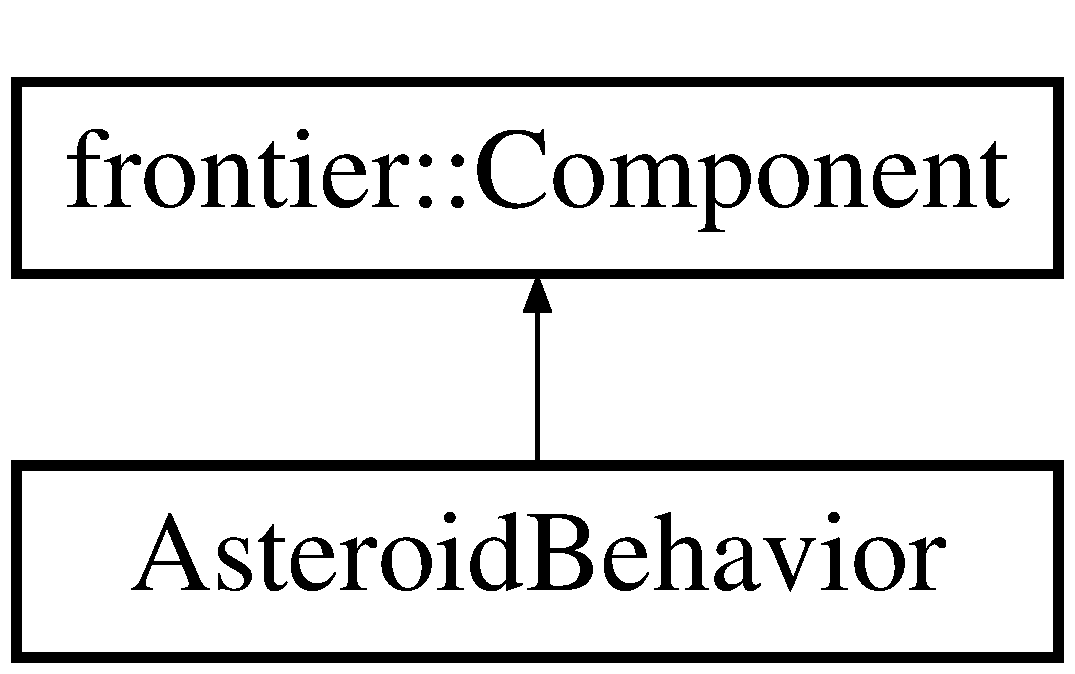
\includegraphics[height=2.000000cm]{class_asteroid_behavior}
\end{center}
\end{figure}
\subsection*{Public Member Functions}
\begin{DoxyCompactItemize}
\item 
void \hyperlink{class_asteroid_behavior_a79d9559f0d8e109e928acf7f8ff7acea}{On\+Init} (std\+::weak\+\_\+ptr$<$ \hyperlink{classfrontier_1_1_entity}{frontier\+::\+Entity} $>$ \+\_\+parent)
\begin{DoxyCompactList}\small\item\em Initialises the component. Sets the pointer to the entity that this component is attached to. \end{DoxyCompactList}\item 
void \hyperlink{class_asteroid_behavior_a3c1287599e132b49be851d9eeec6380e}{On\+Tick} () override
\begin{DoxyCompactList}\small\item\em Called every frame, use for data that needs to be calculated each frame. \end{DoxyCompactList}\item 
void \hyperlink{class_asteroid_behavior_a7c4f344a9461d1296d4dcfcd51ed3bbc}{On\+Activate} () override
\begin{DoxyCompactList}\small\item\em Called when an entity\textquotesingle{}s active state is changed from false to true. \end{DoxyCompactList}\item 
void \hyperlink{class_asteroid_behavior_ab1f0bf83f6291bda3934c1b48141908f}{Set\+Direction} (glm\+::vec3 new\+Direction)
\item 
void \hyperlink{class_asteroid_behavior_a6059686f8a09c3911187407143d3a3cf}{set\+Randomiser\+Override} (bool \+\_\+override)
\end{DoxyCompactItemize}
\subsection*{Additional Inherited Members}


\subsection{Member Function Documentation}
\mbox{\Hypertarget{class_asteroid_behavior_a7c4f344a9461d1296d4dcfcd51ed3bbc}\label{class_asteroid_behavior_a7c4f344a9461d1296d4dcfcd51ed3bbc}} 
\index{Asteroid\+Behavior@{Asteroid\+Behavior}!On\+Activate@{On\+Activate}}
\index{On\+Activate@{On\+Activate}!Asteroid\+Behavior@{Asteroid\+Behavior}}
\subsubsection{\texorpdfstring{On\+Activate()}{OnActivate()}}
{\footnotesize\ttfamily void Asteroid\+Behavior\+::\+On\+Activate (\begin{DoxyParamCaption}{ }\end{DoxyParamCaption})\hspace{0.3cm}{\ttfamily [override]}, {\ttfamily [virtual]}}



Called when an entity\textquotesingle{}s active state is changed from false to true. 



Reimplemented from \hyperlink{classfrontier_1_1_component_a77fca7ba1960aafb9bc05905e300c79d}{frontier\+::\+Component}.

\mbox{\Hypertarget{class_asteroid_behavior_a79d9559f0d8e109e928acf7f8ff7acea}\label{class_asteroid_behavior_a79d9559f0d8e109e928acf7f8ff7acea}} 
\index{Asteroid\+Behavior@{Asteroid\+Behavior}!On\+Init@{On\+Init}}
\index{On\+Init@{On\+Init}!Asteroid\+Behavior@{Asteroid\+Behavior}}
\subsubsection{\texorpdfstring{On\+Init()}{OnInit()}}
{\footnotesize\ttfamily void Asteroid\+Behavior\+::\+On\+Init (\begin{DoxyParamCaption}\item[{std\+::weak\+\_\+ptr$<$ \hyperlink{classfrontier_1_1_entity}{frontier\+::\+Entity} $>$}]{\+\_\+parent }\end{DoxyParamCaption})\hspace{0.3cm}{\ttfamily [virtual]}}



Initialises the component. Sets the pointer to the entity that this component is attached to. 


\begin{DoxyParams}{Parameters}
{\em \+\_\+parent} & The entity that the component will be attached to. \\
\hline
\end{DoxyParams}


Reimplemented from \hyperlink{classfrontier_1_1_component_af3da02905c4d79219d9b12f260a35ad1}{frontier\+::\+Component}.

\mbox{\Hypertarget{class_asteroid_behavior_a3c1287599e132b49be851d9eeec6380e}\label{class_asteroid_behavior_a3c1287599e132b49be851d9eeec6380e}} 
\index{Asteroid\+Behavior@{Asteroid\+Behavior}!On\+Tick@{On\+Tick}}
\index{On\+Tick@{On\+Tick}!Asteroid\+Behavior@{Asteroid\+Behavior}}
\subsubsection{\texorpdfstring{On\+Tick()}{OnTick()}}
{\footnotesize\ttfamily void Asteroid\+Behavior\+::\+On\+Tick (\begin{DoxyParamCaption}{ }\end{DoxyParamCaption})\hspace{0.3cm}{\ttfamily [override]}, {\ttfamily [virtual]}}



Called every frame, use for data that needs to be calculated each frame. 



Reimplemented from \hyperlink{classfrontier_1_1_component_ab920f9bc07ce051ebb5559c5a66508d1}{frontier\+::\+Component}.

\mbox{\Hypertarget{class_asteroid_behavior_ab1f0bf83f6291bda3934c1b48141908f}\label{class_asteroid_behavior_ab1f0bf83f6291bda3934c1b48141908f}} 
\index{Asteroid\+Behavior@{Asteroid\+Behavior}!Set\+Direction@{Set\+Direction}}
\index{Set\+Direction@{Set\+Direction}!Asteroid\+Behavior@{Asteroid\+Behavior}}
\subsubsection{\texorpdfstring{Set\+Direction()}{SetDirection()}}
{\footnotesize\ttfamily void Asteroid\+Behavior\+::\+Set\+Direction (\begin{DoxyParamCaption}\item[{glm\+::vec3}]{new\+Direction }\end{DoxyParamCaption})}

\mbox{\Hypertarget{class_asteroid_behavior_a6059686f8a09c3911187407143d3a3cf}\label{class_asteroid_behavior_a6059686f8a09c3911187407143d3a3cf}} 
\index{Asteroid\+Behavior@{Asteroid\+Behavior}!set\+Randomiser\+Override@{set\+Randomiser\+Override}}
\index{set\+Randomiser\+Override@{set\+Randomiser\+Override}!Asteroid\+Behavior@{Asteroid\+Behavior}}
\subsubsection{\texorpdfstring{set\+Randomiser\+Override()}{setRandomiserOverride()}}
{\footnotesize\ttfamily void Asteroid\+Behavior\+::set\+Randomiser\+Override (\begin{DoxyParamCaption}\item[{bool}]{\+\_\+override }\end{DoxyParamCaption})}



The documentation for this class was generated from the following files\+:\begin{DoxyCompactItemize}
\item 
src/game/\hyperlink{_asteroid_behavior_8h}{Asteroid\+Behavior.\+h}\item 
src/game/\hyperlink{_asteroid_behavior_8cpp}{Asteroid\+Behavior.\+cpp}\end{DoxyCompactItemize}

\hypertarget{class_asteroid_spawner}{}\section{Asteroid\+Spawner Class Reference}
\label{class_asteroid_spawner}\index{Asteroid\+Spawner@{Asteroid\+Spawner}}


{\ttfamily \#include $<$Asteroid\+Spawner.\+h$>$}

Inheritance diagram for Asteroid\+Spawner\+:\begin{figure}[H]
\begin{center}
\leavevmode
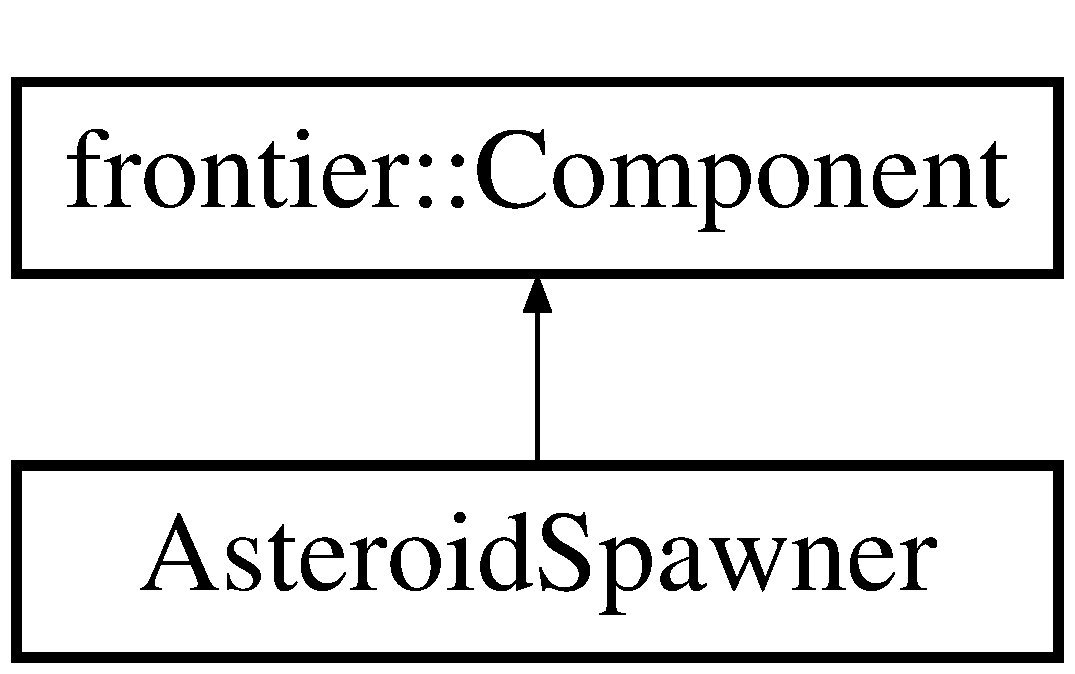
\includegraphics[height=2.000000cm]{class_asteroid_spawner}
\end{center}
\end{figure}
\subsection*{Public Member Functions}
\begin{DoxyCompactItemize}
\item 
void \hyperlink{class_asteroid_spawner_a55785f3beb7478604241becaacb266a3}{On\+Init} (std\+::weak\+\_\+ptr$<$ \hyperlink{classfrontier_1_1_entity}{frontier\+::\+Entity} $>$ \+\_\+parent, std\+::weak\+\_\+ptr$<$ \hyperlink{classfrontier_1_1_pooler}{frontier\+::\+Pooler} $>$ \+\_\+asteroid\+Pooler)
\item 
void \hyperlink{class_asteroid_spawner_acd2744a9a1ac8f13ac28220b33b9f750}{On\+Tick} () override
\item 
void \hyperlink{class_asteroid_spawner_a4ba8146f631d20b3f293f05cb6542da5}{Set\+Player} (std\+::weak\+\_\+ptr$<$ \hyperlink{classfrontier_1_1_entity}{frontier\+::\+Entity} $>$ \+\_\+player)
\end{DoxyCompactItemize}
\subsection*{Additional Inherited Members}


\subsection{Member Function Documentation}
\mbox{\Hypertarget{class_asteroid_spawner_a55785f3beb7478604241becaacb266a3}\label{class_asteroid_spawner_a55785f3beb7478604241becaacb266a3}} 
\index{Asteroid\+Spawner@{Asteroid\+Spawner}!On\+Init@{On\+Init}}
\index{On\+Init@{On\+Init}!Asteroid\+Spawner@{Asteroid\+Spawner}}
\subsubsection{\texorpdfstring{On\+Init()}{OnInit()}}
{\footnotesize\ttfamily void Asteroid\+Spawner\+::\+On\+Init (\begin{DoxyParamCaption}\item[{std\+::weak\+\_\+ptr$<$ \hyperlink{classfrontier_1_1_entity}{frontier\+::\+Entity} $>$}]{\+\_\+parent,  }\item[{std\+::weak\+\_\+ptr$<$ \hyperlink{classfrontier_1_1_pooler}{frontier\+::\+Pooler} $>$}]{\+\_\+asteroid\+Pooler }\end{DoxyParamCaption})}

\mbox{\Hypertarget{class_asteroid_spawner_acd2744a9a1ac8f13ac28220b33b9f750}\label{class_asteroid_spawner_acd2744a9a1ac8f13ac28220b33b9f750}} 
\index{Asteroid\+Spawner@{Asteroid\+Spawner}!On\+Tick@{On\+Tick}}
\index{On\+Tick@{On\+Tick}!Asteroid\+Spawner@{Asteroid\+Spawner}}
\subsubsection{\texorpdfstring{On\+Tick()}{OnTick()}}
{\footnotesize\ttfamily void Asteroid\+Spawner\+::\+On\+Tick (\begin{DoxyParamCaption}{ }\end{DoxyParamCaption})\hspace{0.3cm}{\ttfamily [override]}, {\ttfamily [virtual]}}



Reimplemented from \hyperlink{classfrontier_1_1_component_ab920f9bc07ce051ebb5559c5a66508d1}{frontier\+::\+Component}.

\mbox{\Hypertarget{class_asteroid_spawner_a4ba8146f631d20b3f293f05cb6542da5}\label{class_asteroid_spawner_a4ba8146f631d20b3f293f05cb6542da5}} 
\index{Asteroid\+Spawner@{Asteroid\+Spawner}!Set\+Player@{Set\+Player}}
\index{Set\+Player@{Set\+Player}!Asteroid\+Spawner@{Asteroid\+Spawner}}
\subsubsection{\texorpdfstring{Set\+Player()}{SetPlayer()}}
{\footnotesize\ttfamily void Asteroid\+Spawner\+::\+Set\+Player (\begin{DoxyParamCaption}\item[{std\+::weak\+\_\+ptr$<$ \hyperlink{classfrontier_1_1_entity}{frontier\+::\+Entity} $>$}]{\+\_\+player }\end{DoxyParamCaption})}



The documentation for this class was generated from the following files\+:\begin{DoxyCompactItemize}
\item 
src/game/\hyperlink{_asteroid_spawner_8h}{Asteroid\+Spawner.\+h}\item 
src/game/\hyperlink{_asteroid_spawner_8cpp}{Asteroid\+Spawner.\+cpp}\end{DoxyCompactItemize}

\hypertarget{classfrontier_1_1_audio_player}{}\section{frontier\+:\+:Audio\+Player Class Reference}
\label{classfrontier_1_1_audio_player}\index{frontier\+::\+Audio\+Player@{frontier\+::\+Audio\+Player}}


This class holds a sound resource which can then be attached to a entity can can be played in various different ways.  




{\ttfamily \#include $<$Audio\+Player.\+h$>$}

Inheritance diagram for frontier\+:\+:Audio\+Player\+:\begin{figure}[H]
\begin{center}
\leavevmode
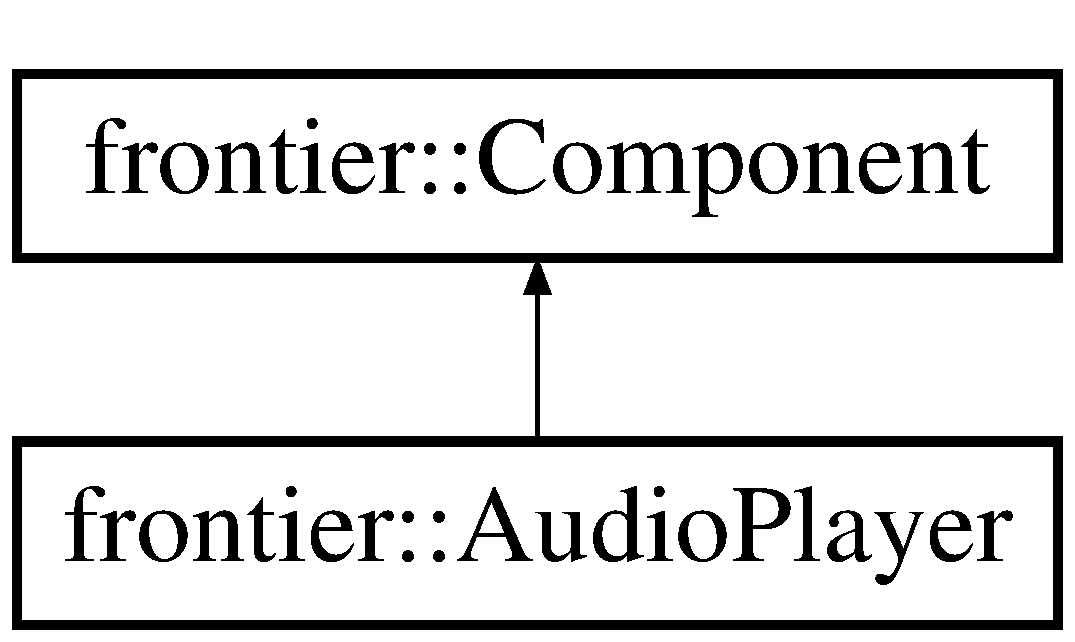
\includegraphics[height=2.000000cm]{classfrontier_1_1_audio_player}
\end{center}
\end{figure}
\subsection*{Public Member Functions}
\begin{DoxyCompactItemize}
\item 
void \hyperlink{classfrontier_1_1_audio_player_a6a000a15e398c4de2eb767c4a4cbede7}{On\+Init} (std\+::weak\+\_\+ptr$<$ \hyperlink{classfrontier_1_1_entity}{Entity} $>$ \+\_\+parent, std\+::shared\+\_\+ptr$<$ \hyperlink{classfrontier_1_1_sound}{Sound} $>$ \+\_\+sound)
\begin{DoxyCompactList}\small\item\em Initialises the audio player component, this will be called by Add\+Component in the \hyperlink{classfrontier_1_1_entity}{Entity} class, adds a sound to the audio player. \end{DoxyCompactList}\item 
void \hyperlink{classfrontier_1_1_audio_player_ad5791ca0776113116a815f86bd630ad7}{Play} (bool \+\_\+looping=false)
\begin{DoxyCompactList}\small\item\em Plays the currently attached sound. \end{DoxyCompactList}\item 
void \hyperlink{classfrontier_1_1_audio_player_a757be1bd81df8c3885b03177946b38d1}{Play} (glm\+::vec3 \+\_\+sound\+Position, glm\+::vec3 \+\_\+listener\+Position, bool \+\_\+looping=false)
\begin{DoxyCompactList}\small\item\em Plays the currently attached sound. \end{DoxyCompactList}\item 
void \hyperlink{classfrontier_1_1_audio_player_ad26964a251fa785cacd76617efa92ee3}{Play\+With\+Variance} (float \+\_\+vol, float \+\_\+var\+Min, float \+\_\+var\+Max)
\begin{DoxyCompactList}\small\item\em Plays the currently attached sound with the pitch shifted randomly between the two provided floats. \end{DoxyCompactList}\item 
void \hyperlink{classfrontier_1_1_audio_player_abb7536bee69926c8643a9c3ab6eb714f}{Attach\+Sound} (std\+::shared\+\_\+ptr$<$ \hyperlink{classfrontier_1_1_sound}{Sound} $>$ \+\_\+sound)
\begin{DoxyCompactList}\small\item\em Attaches a new sound to the audio player. \end{DoxyCompactList}\item 
void \hyperlink{classfrontier_1_1_audio_player_a0e22a78d69571eac70811c8457eeda50}{Stop} ()
\begin{DoxyCompactList}\small\item\em Stops playing the sound. \end{DoxyCompactList}\end{DoxyCompactItemize}
\subsection*{Additional Inherited Members}


\subsection{Detailed Description}
This class holds a sound resource which can then be attached to a entity can can be played in various different ways. 

\subsection{Member Function Documentation}
\mbox{\Hypertarget{classfrontier_1_1_audio_player_abb7536bee69926c8643a9c3ab6eb714f}\label{classfrontier_1_1_audio_player_abb7536bee69926c8643a9c3ab6eb714f}} 
\index{frontier\+::\+Audio\+Player@{frontier\+::\+Audio\+Player}!Attach\+Sound@{Attach\+Sound}}
\index{Attach\+Sound@{Attach\+Sound}!frontier\+::\+Audio\+Player@{frontier\+::\+Audio\+Player}}
\subsubsection{\texorpdfstring{Attach\+Sound()}{AttachSound()}}
{\footnotesize\ttfamily void frontier\+::\+Audio\+Player\+::\+Attach\+Sound (\begin{DoxyParamCaption}\item[{std\+::shared\+\_\+ptr$<$ \hyperlink{classfrontier_1_1_sound}{Sound} $>$}]{\+\_\+sound }\end{DoxyParamCaption})}



Attaches a new sound to the audio player. 


\begin{DoxyParams}{Parameters}
{\em \+\_\+sound} & The new sound to be attached to the audio player. \\
\hline
\end{DoxyParams}
\mbox{\Hypertarget{classfrontier_1_1_audio_player_a6a000a15e398c4de2eb767c4a4cbede7}\label{classfrontier_1_1_audio_player_a6a000a15e398c4de2eb767c4a4cbede7}} 
\index{frontier\+::\+Audio\+Player@{frontier\+::\+Audio\+Player}!On\+Init@{On\+Init}}
\index{On\+Init@{On\+Init}!frontier\+::\+Audio\+Player@{frontier\+::\+Audio\+Player}}
\subsubsection{\texorpdfstring{On\+Init()}{OnInit()}}
{\footnotesize\ttfamily void frontier\+::\+Audio\+Player\+::\+On\+Init (\begin{DoxyParamCaption}\item[{std\+::weak\+\_\+ptr$<$ \hyperlink{classfrontier_1_1_entity}{Entity} $>$}]{\+\_\+parent,  }\item[{std\+::shared\+\_\+ptr$<$ \hyperlink{classfrontier_1_1_sound}{Sound} $>$}]{\+\_\+sound }\end{DoxyParamCaption})}



Initialises the audio player component, this will be called by Add\+Component in the \hyperlink{classfrontier_1_1_entity}{Entity} class, adds a sound to the audio player. 


\begin{DoxyParams}{Parameters}
{\em \+\_\+parent} & The entity that this component is attached to. \\
\hline
{\em \+\_\+sound} & The sound that will be played by this audio player component. \\
\hline
\end{DoxyParams}
\mbox{\Hypertarget{classfrontier_1_1_audio_player_ad5791ca0776113116a815f86bd630ad7}\label{classfrontier_1_1_audio_player_ad5791ca0776113116a815f86bd630ad7}} 
\index{frontier\+::\+Audio\+Player@{frontier\+::\+Audio\+Player}!Play@{Play}}
\index{Play@{Play}!frontier\+::\+Audio\+Player@{frontier\+::\+Audio\+Player}}
\subsubsection{\texorpdfstring{Play()}{Play()}\hspace{0.1cm}{\footnotesize\ttfamily [1/2]}}
{\footnotesize\ttfamily void frontier\+::\+Audio\+Player\+::\+Play (\begin{DoxyParamCaption}\item[{bool}]{\+\_\+looping = {\ttfamily false} }\end{DoxyParamCaption})}



Plays the currently attached sound. 


\begin{DoxyParams}{Parameters}
{\em \+\_\+looping} & Whether the audio source will play continuously on a loop (Set to false by default). \\
\hline
\end{DoxyParams}
\mbox{\Hypertarget{classfrontier_1_1_audio_player_a757be1bd81df8c3885b03177946b38d1}\label{classfrontier_1_1_audio_player_a757be1bd81df8c3885b03177946b38d1}} 
\index{frontier\+::\+Audio\+Player@{frontier\+::\+Audio\+Player}!Play@{Play}}
\index{Play@{Play}!frontier\+::\+Audio\+Player@{frontier\+::\+Audio\+Player}}
\subsubsection{\texorpdfstring{Play()}{Play()}\hspace{0.1cm}{\footnotesize\ttfamily [2/2]}}
{\footnotesize\ttfamily void frontier\+::\+Audio\+Player\+::\+Play (\begin{DoxyParamCaption}\item[{glm\+::vec3}]{\+\_\+sound\+Position,  }\item[{glm\+::vec3}]{\+\_\+listener\+Position,  }\item[{bool}]{\+\_\+looping = {\ttfamily false} }\end{DoxyParamCaption})}



Plays the currently attached sound. 


\begin{DoxyParams}{Parameters}
{\em \+\_\+sound\+Position} & Where the sound will play from. \\
\hline
{\em \+\_\+listener\+Position} & Where the sound will be heard from. \\
\hline
{\em \+\_\+looping} & Whether the audio source will play continuously on a loop. \\
\hline
\end{DoxyParams}
\mbox{\Hypertarget{classfrontier_1_1_audio_player_ad26964a251fa785cacd76617efa92ee3}\label{classfrontier_1_1_audio_player_ad26964a251fa785cacd76617efa92ee3}} 
\index{frontier\+::\+Audio\+Player@{frontier\+::\+Audio\+Player}!Play\+With\+Variance@{Play\+With\+Variance}}
\index{Play\+With\+Variance@{Play\+With\+Variance}!frontier\+::\+Audio\+Player@{frontier\+::\+Audio\+Player}}
\subsubsection{\texorpdfstring{Play\+With\+Variance()}{PlayWithVariance()}}
{\footnotesize\ttfamily void frontier\+::\+Audio\+Player\+::\+Play\+With\+Variance (\begin{DoxyParamCaption}\item[{float}]{\+\_\+vol,  }\item[{float}]{\+\_\+var\+Min,  }\item[{float}]{\+\_\+var\+Max }\end{DoxyParamCaption})}



Plays the currently attached sound with the pitch shifted randomly between the two provided floats. 


\begin{DoxyParams}{Parameters}
{\em \+\_\+vol} & The volume of the audio. \\
\hline
{\em \+\_\+var\+Min} & The minimum value on the variance. \\
\hline
{\em \+\_\+var\+Max} & The maximum value on the variance. \\
\hline
\end{DoxyParams}
\mbox{\Hypertarget{classfrontier_1_1_audio_player_a0e22a78d69571eac70811c8457eeda50}\label{classfrontier_1_1_audio_player_a0e22a78d69571eac70811c8457eeda50}} 
\index{frontier\+::\+Audio\+Player@{frontier\+::\+Audio\+Player}!Stop@{Stop}}
\index{Stop@{Stop}!frontier\+::\+Audio\+Player@{frontier\+::\+Audio\+Player}}
\subsubsection{\texorpdfstring{Stop()}{Stop()}}
{\footnotesize\ttfamily void frontier\+::\+Audio\+Player\+::\+Stop (\begin{DoxyParamCaption}{ }\end{DoxyParamCaption})}



Stops playing the sound. 



The documentation for this class was generated from the following files\+:\begin{DoxyCompactItemize}
\item 
src/myengine/\hyperlink{_audio_player_8h}{Audio\+Player.\+h}\item 
src/myengine/\hyperlink{_audio_player_8cpp}{Audio\+Player.\+cpp}\end{DoxyCompactItemize}

\hypertarget{classfrontier_1_1_back_ground_color}{}\section{frontier\+:\+:Back\+Ground\+Color Class Reference}
\label{classfrontier_1_1_back_ground_color}\index{frontier\+::\+Back\+Ground\+Color@{frontier\+::\+Back\+Ground\+Color}}


{\ttfamily \#include $<$Background\+Color.\+h$>$}

Inheritance diagram for frontier\+:\+:Back\+Ground\+Color\+:\begin{figure}[H]
\begin{center}
\leavevmode
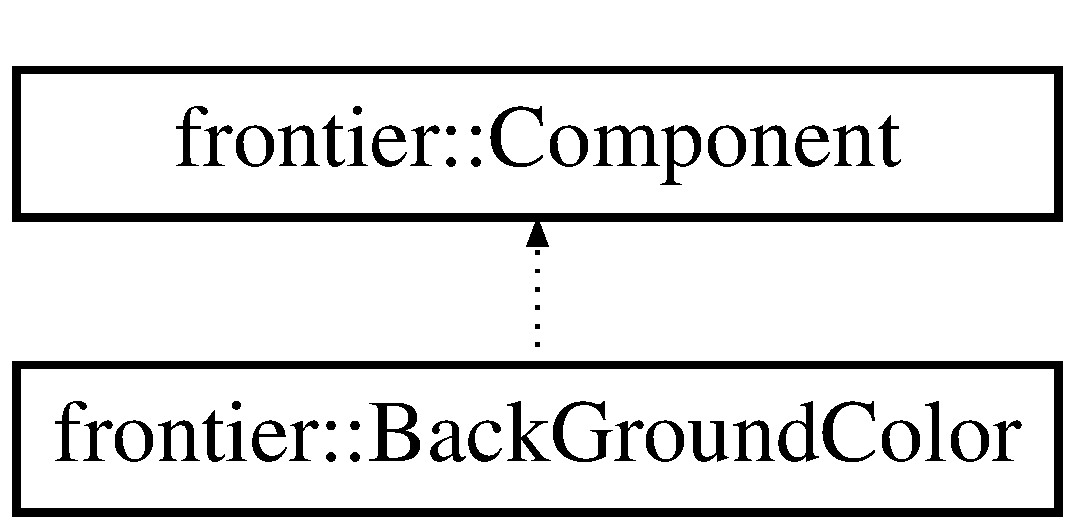
\includegraphics[height=2.000000cm]{classfrontier_1_1_back_ground_color}
\end{center}
\end{figure}


The documentation for this class was generated from the following file\+:\begin{DoxyCompactItemize}
\item 
src/myengine/\hyperlink{_background_color_8h}{Background\+Color.\+h}\end{DoxyCompactItemize}

\hypertarget{classfrontier_1_1_camera}{}\section{frontier\+:\+:Camera Class Reference}
\label{classfrontier_1_1_camera}\index{frontier\+::\+Camera@{frontier\+::\+Camera}}


{\ttfamily \#include $<$Camera.\+h$>$}

Inheritance diagram for frontier\+:\+:Camera\+:\begin{figure}[H]
\begin{center}
\leavevmode
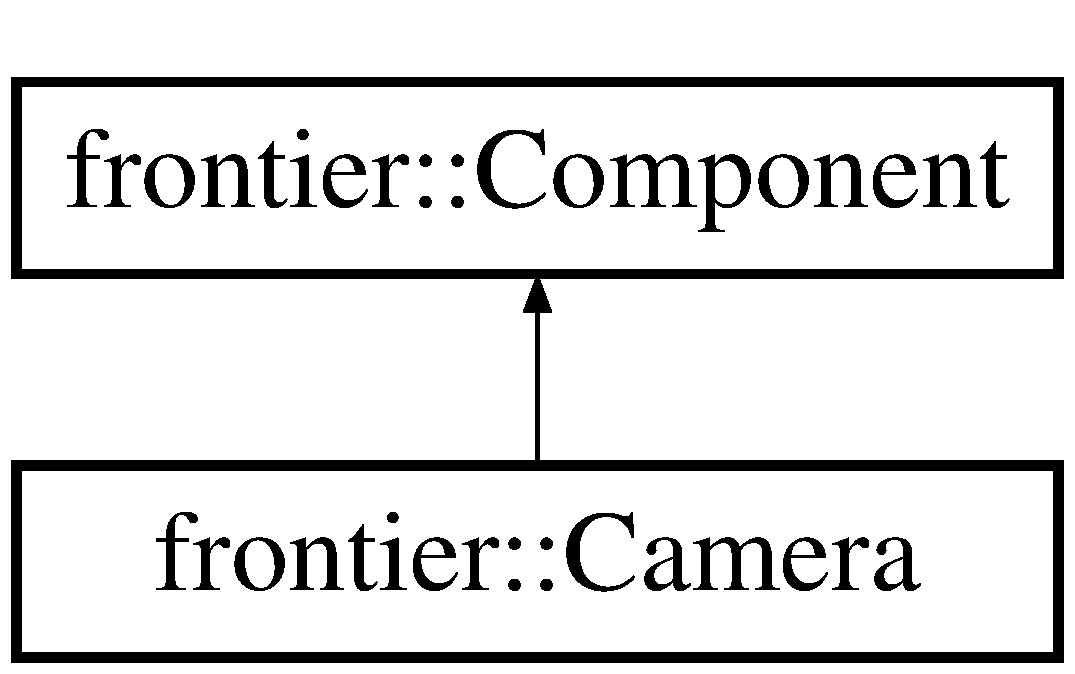
\includegraphics[height=2.000000cm]{classfrontier_1_1_camera}
\end{center}
\end{figure}
\subsection*{Public Member Functions}
\begin{DoxyCompactItemize}
\item 
glm\+::mat4 \hyperlink{classfrontier_1_1_camera_a90858bfacddb80bedb062889b15d2d47}{get\+View\+Matrix} ()
\item 
glm\+::mat4 \hyperlink{classfrontier_1_1_camera_ae3e5871e68bcb0d5577cc09b2273c641}{get\+Projection\+Matrix} ()
\item 
glm\+::mat4 \hyperlink{classfrontier_1_1_camera_a7c5d631b29e93e4e8772577dd3e62378}{get\+Orthographic\+Matrix} ()
\item 
void \hyperlink{classfrontier_1_1_camera_a7bec1b9133e266bf50396883cb3e2b83}{On\+Init} (std\+::weak\+\_\+ptr$<$ \hyperlink{classfrontier_1_1_entity}{Entity} $>$ \+\_\+parent, float fov, float near, float far)
\item 
bool \hyperlink{classfrontier_1_1_camera_a8e6077e5c7dd76f58e055a13e18ab8c6}{get\+Main} ()
\item 
void \hyperlink{classfrontier_1_1_camera_ae8a9b95bf6e4eacdae709d188725e72a}{set\+Main} (bool \hyperlink{main_8cpp_ae66f6b31b5ad750f1fe042a706a4e3d4}{main})
\item 
void \hyperlink{classfrontier_1_1_camera_ab1872f3ceccbb6dcfa4fcf043f0eb5f8}{set\+Controllable} (bool \+\_\+control)
\item 
void \hyperlink{classfrontier_1_1_camera_a1f318703a68e4c070c85a1d9a27446d0}{On\+Tick} () override
\end{DoxyCompactItemize}
\subsection*{Additional Inherited Members}


\subsection{Member Function Documentation}
\mbox{\Hypertarget{classfrontier_1_1_camera_a8e6077e5c7dd76f58e055a13e18ab8c6}\label{classfrontier_1_1_camera_a8e6077e5c7dd76f58e055a13e18ab8c6}} 
\index{frontier\+::\+Camera@{frontier\+::\+Camera}!get\+Main@{get\+Main}}
\index{get\+Main@{get\+Main}!frontier\+::\+Camera@{frontier\+::\+Camera}}
\subsubsection{\texorpdfstring{get\+Main()}{getMain()}}
{\footnotesize\ttfamily bool frontier\+::\+Camera\+::get\+Main (\begin{DoxyParamCaption}{ }\end{DoxyParamCaption})}

\mbox{\Hypertarget{classfrontier_1_1_camera_a7c5d631b29e93e4e8772577dd3e62378}\label{classfrontier_1_1_camera_a7c5d631b29e93e4e8772577dd3e62378}} 
\index{frontier\+::\+Camera@{frontier\+::\+Camera}!get\+Orthographic\+Matrix@{get\+Orthographic\+Matrix}}
\index{get\+Orthographic\+Matrix@{get\+Orthographic\+Matrix}!frontier\+::\+Camera@{frontier\+::\+Camera}}
\subsubsection{\texorpdfstring{get\+Orthographic\+Matrix()}{getOrthographicMatrix()}}
{\footnotesize\ttfamily glm\+::mat4 frontier\+::\+Camera\+::get\+Orthographic\+Matrix (\begin{DoxyParamCaption}{ }\end{DoxyParamCaption})}

\mbox{\Hypertarget{classfrontier_1_1_camera_ae3e5871e68bcb0d5577cc09b2273c641}\label{classfrontier_1_1_camera_ae3e5871e68bcb0d5577cc09b2273c641}} 
\index{frontier\+::\+Camera@{frontier\+::\+Camera}!get\+Projection\+Matrix@{get\+Projection\+Matrix}}
\index{get\+Projection\+Matrix@{get\+Projection\+Matrix}!frontier\+::\+Camera@{frontier\+::\+Camera}}
\subsubsection{\texorpdfstring{get\+Projection\+Matrix()}{getProjectionMatrix()}}
{\footnotesize\ttfamily glm\+::mat4 frontier\+::\+Camera\+::get\+Projection\+Matrix (\begin{DoxyParamCaption}{ }\end{DoxyParamCaption})}

\mbox{\Hypertarget{classfrontier_1_1_camera_a90858bfacddb80bedb062889b15d2d47}\label{classfrontier_1_1_camera_a90858bfacddb80bedb062889b15d2d47}} 
\index{frontier\+::\+Camera@{frontier\+::\+Camera}!get\+View\+Matrix@{get\+View\+Matrix}}
\index{get\+View\+Matrix@{get\+View\+Matrix}!frontier\+::\+Camera@{frontier\+::\+Camera}}
\subsubsection{\texorpdfstring{get\+View\+Matrix()}{getViewMatrix()}}
{\footnotesize\ttfamily glm\+::mat4 frontier\+::\+Camera\+::get\+View\+Matrix (\begin{DoxyParamCaption}{ }\end{DoxyParamCaption})}

\mbox{\Hypertarget{classfrontier_1_1_camera_a7bec1b9133e266bf50396883cb3e2b83}\label{classfrontier_1_1_camera_a7bec1b9133e266bf50396883cb3e2b83}} 
\index{frontier\+::\+Camera@{frontier\+::\+Camera}!On\+Init@{On\+Init}}
\index{On\+Init@{On\+Init}!frontier\+::\+Camera@{frontier\+::\+Camera}}
\subsubsection{\texorpdfstring{On\+Init()}{OnInit()}}
{\footnotesize\ttfamily void frontier\+::\+Camera\+::\+On\+Init (\begin{DoxyParamCaption}\item[{std\+::weak\+\_\+ptr$<$ \hyperlink{classfrontier_1_1_entity}{Entity} $>$}]{\+\_\+parent,  }\item[{float}]{fov,  }\item[{float}]{near,  }\item[{float}]{far }\end{DoxyParamCaption})}

\mbox{\Hypertarget{classfrontier_1_1_camera_a1f318703a68e4c070c85a1d9a27446d0}\label{classfrontier_1_1_camera_a1f318703a68e4c070c85a1d9a27446d0}} 
\index{frontier\+::\+Camera@{frontier\+::\+Camera}!On\+Tick@{On\+Tick}}
\index{On\+Tick@{On\+Tick}!frontier\+::\+Camera@{frontier\+::\+Camera}}
\subsubsection{\texorpdfstring{On\+Tick()}{OnTick()}}
{\footnotesize\ttfamily void frontier\+::\+Camera\+::\+On\+Tick (\begin{DoxyParamCaption}{ }\end{DoxyParamCaption})\hspace{0.3cm}{\ttfamily [override]}, {\ttfamily [virtual]}}



Reimplemented from \hyperlink{classfrontier_1_1_component_ab920f9bc07ce051ebb5559c5a66508d1}{frontier\+::\+Component}.

\mbox{\Hypertarget{classfrontier_1_1_camera_ab1872f3ceccbb6dcfa4fcf043f0eb5f8}\label{classfrontier_1_1_camera_ab1872f3ceccbb6dcfa4fcf043f0eb5f8}} 
\index{frontier\+::\+Camera@{frontier\+::\+Camera}!set\+Controllable@{set\+Controllable}}
\index{set\+Controllable@{set\+Controllable}!frontier\+::\+Camera@{frontier\+::\+Camera}}
\subsubsection{\texorpdfstring{set\+Controllable()}{setControllable()}}
{\footnotesize\ttfamily void frontier\+::\+Camera\+::set\+Controllable (\begin{DoxyParamCaption}\item[{bool}]{\+\_\+control }\end{DoxyParamCaption})}

\mbox{\Hypertarget{classfrontier_1_1_camera_ae8a9b95bf6e4eacdae709d188725e72a}\label{classfrontier_1_1_camera_ae8a9b95bf6e4eacdae709d188725e72a}} 
\index{frontier\+::\+Camera@{frontier\+::\+Camera}!set\+Main@{set\+Main}}
\index{set\+Main@{set\+Main}!frontier\+::\+Camera@{frontier\+::\+Camera}}
\subsubsection{\texorpdfstring{set\+Main()}{setMain()}}
{\footnotesize\ttfamily void frontier\+::\+Camera\+::set\+Main (\begin{DoxyParamCaption}\item[{bool}]{main }\end{DoxyParamCaption})}



The documentation for this class was generated from the following files\+:\begin{DoxyCompactItemize}
\item 
src/myengine/\hyperlink{_camera_8h}{Camera.\+h}\item 
src/myengine/\hyperlink{_camera_8cpp}{Camera.\+cpp}\end{DoxyCompactItemize}

\hypertarget{classfrontier_1_1_collider}{}\section{frontier\+:\+:Collider Class Reference}
\label{classfrontier_1_1_collider}\index{frontier\+::\+Collider@{frontier\+::\+Collider}}


A box collider, uses basic A\+A\+BB collisions against other entities with a collider attached.  




{\ttfamily \#include $<$Collider.\+h$>$}

Inheritance diagram for frontier\+:\+:Collider\+:\begin{figure}[H]
\begin{center}
\leavevmode
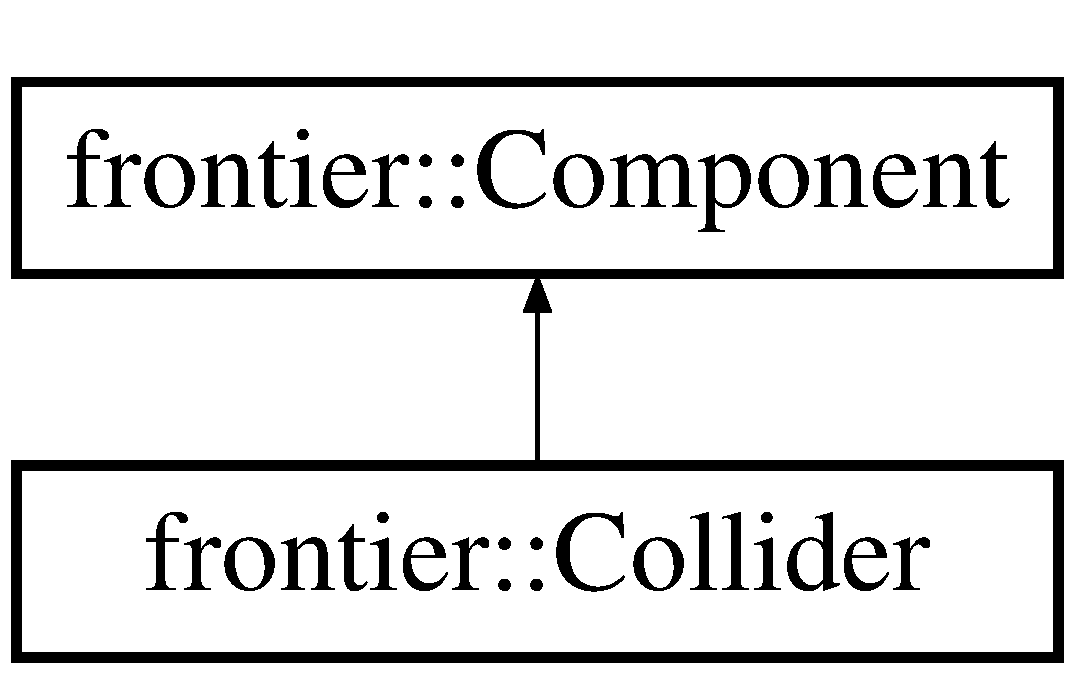
\includegraphics[height=2.000000cm]{classfrontier_1_1_collider}
\end{center}
\end{figure}
\subsection*{Public Member Functions}
\begin{DoxyCompactItemize}
\item 
void \hyperlink{classfrontier_1_1_collider_aa11b97036f0962e2abcb79b4d84b8687}{On\+Init} (std\+::weak\+\_\+ptr$<$ \hyperlink{classfrontier_1_1_entity}{Entity} $>$ \+\_\+parent, glm\+::vec3 \+\_\+box\+Scale=glm\+::vec3(1.\+0f, 1.\+0f, 1.\+0f))
\begin{DoxyCompactList}\small\item\em Initialises the collider component, this will be called by Add\+Component in the \hyperlink{classfrontier_1_1_entity}{Entity} class, intialises the collider class with the box scale. \end{DoxyCompactList}\item 
void \hyperlink{classfrontier_1_1_collider_a06dfeb56017f45597f1812fc5cf8236d}{On\+Init} (std\+::weak\+\_\+ptr$<$ \hyperlink{classfrontier_1_1_entity}{Entity} $>$ \+\_\+parent, std\+::weak\+\_\+ptr$<$ \hyperlink{classfrontier_1_1_collider}{Collider} $>$ \+\_\+original)
\begin{DoxyCompactList}\small\item\em Initialises the collider component, this will be called by Add\+Component in the \hyperlink{classfrontier_1_1_entity}{Entity} class, this is a copy contructor used for making an entity from a prefab. \end{DoxyCompactList}\item 
void \hyperlink{classfrontier_1_1_collider_ac03782c94e8f7a2064ea1441cbd12c81}{On\+Tick} () override
\begin{DoxyCompactList}\small\item\em Runs every frame, checks all other collider components to see if any are colliding. \end{DoxyCompactList}\item 
bool \hyperlink{classfrontier_1_1_collider_aa0269702eb2d87a12087e933821ad6e0}{Check\+If\+Colliding} (glm\+::vec3 \+\_\+position, glm\+::vec3 \+\_\+scale)
\begin{DoxyCompactList}\small\item\em Checks against another entity\textquotesingle{}s position and scale to determine whether this collider is collding with another. \end{DoxyCompactList}\item 
std\+::vector$<$ std\+::weak\+\_\+ptr$<$ \hyperlink{classfrontier_1_1_entity}{Entity} $>$ $>$ \hyperlink{classfrontier_1_1_collider_a95ae710a5b6e370fc79967ff650f2f6f}{Get\+Colliding\+Entities} ()
\begin{DoxyCompactList}\small\item\em Returns the vector of entities currently colliding with this collider. \end{DoxyCompactList}\item 
bool \hyperlink{classfrontier_1_1_collider_abcc4976d3ac48d591a0e725fb457260a}{Is\+Colliding} ()
\begin{DoxyCompactList}\small\item\em Returns whether the collider is currently colliding with anything. \end{DoxyCompactList}\item 
glm\+::vec3 \hyperlink{classfrontier_1_1_collider_a2f8285a81d952b72bf0a02703f7d3481}{Get\+Box\+Scale} ()
\begin{DoxyCompactList}\small\item\em Returns the box scale. \end{DoxyCompactList}\end{DoxyCompactItemize}
\subsection*{Additional Inherited Members}


\subsection{Detailed Description}
A box collider, uses basic A\+A\+BB collisions against other entities with a collider attached. 

If other colliders are intersecting, then the collider component will trigger a boolean to confirm the collsion and will store a vector of weak pointers to each entity colliding with this one. Currently the collider only works based on positions and scale, rotations are not applied. 

\subsection{Member Function Documentation}
\mbox{\Hypertarget{classfrontier_1_1_collider_aa0269702eb2d87a12087e933821ad6e0}\label{classfrontier_1_1_collider_aa0269702eb2d87a12087e933821ad6e0}} 
\index{frontier\+::\+Collider@{frontier\+::\+Collider}!Check\+If\+Colliding@{Check\+If\+Colliding}}
\index{Check\+If\+Colliding@{Check\+If\+Colliding}!frontier\+::\+Collider@{frontier\+::\+Collider}}
\subsubsection{\texorpdfstring{Check\+If\+Colliding()}{CheckIfColliding()}}
{\footnotesize\ttfamily bool frontier\+::\+Collider\+::\+Check\+If\+Colliding (\begin{DoxyParamCaption}\item[{glm\+::vec3}]{\+\_\+position,  }\item[{glm\+::vec3}]{\+\_\+scale }\end{DoxyParamCaption})}



Checks against another entity\textquotesingle{}s position and scale to determine whether this collider is collding with another. 


\begin{DoxyParams}{Parameters}
{\em \+\_\+position} & The position of the other entity. \\
\hline
{\em \+\_\+scale} & The scale of the other entity. \\
\hline
\end{DoxyParams}
\mbox{\Hypertarget{classfrontier_1_1_collider_a2f8285a81d952b72bf0a02703f7d3481}\label{classfrontier_1_1_collider_a2f8285a81d952b72bf0a02703f7d3481}} 
\index{frontier\+::\+Collider@{frontier\+::\+Collider}!Get\+Box\+Scale@{Get\+Box\+Scale}}
\index{Get\+Box\+Scale@{Get\+Box\+Scale}!frontier\+::\+Collider@{frontier\+::\+Collider}}
\subsubsection{\texorpdfstring{Get\+Box\+Scale()}{GetBoxScale()}}
{\footnotesize\ttfamily glm\+::vec3 frontier\+::\+Collider\+::\+Get\+Box\+Scale (\begin{DoxyParamCaption}{ }\end{DoxyParamCaption})}



Returns the box scale. 

\mbox{\Hypertarget{classfrontier_1_1_collider_a95ae710a5b6e370fc79967ff650f2f6f}\label{classfrontier_1_1_collider_a95ae710a5b6e370fc79967ff650f2f6f}} 
\index{frontier\+::\+Collider@{frontier\+::\+Collider}!Get\+Colliding\+Entities@{Get\+Colliding\+Entities}}
\index{Get\+Colliding\+Entities@{Get\+Colliding\+Entities}!frontier\+::\+Collider@{frontier\+::\+Collider}}
\subsubsection{\texorpdfstring{Get\+Colliding\+Entities()}{GetCollidingEntities()}}
{\footnotesize\ttfamily std\+::vector$<$ std\+::weak\+\_\+ptr$<$ \hyperlink{classfrontier_1_1_entity}{Entity} $>$ $>$ frontier\+::\+Collider\+::\+Get\+Colliding\+Entities (\begin{DoxyParamCaption}{ }\end{DoxyParamCaption})}



Returns the vector of entities currently colliding with this collider. 

\mbox{\Hypertarget{classfrontier_1_1_collider_abcc4976d3ac48d591a0e725fb457260a}\label{classfrontier_1_1_collider_abcc4976d3ac48d591a0e725fb457260a}} 
\index{frontier\+::\+Collider@{frontier\+::\+Collider}!Is\+Colliding@{Is\+Colliding}}
\index{Is\+Colliding@{Is\+Colliding}!frontier\+::\+Collider@{frontier\+::\+Collider}}
\subsubsection{\texorpdfstring{Is\+Colliding()}{IsColliding()}}
{\footnotesize\ttfamily bool frontier\+::\+Collider\+::\+Is\+Colliding (\begin{DoxyParamCaption}{ }\end{DoxyParamCaption})}



Returns whether the collider is currently colliding with anything. 

\mbox{\Hypertarget{classfrontier_1_1_collider_aa11b97036f0962e2abcb79b4d84b8687}\label{classfrontier_1_1_collider_aa11b97036f0962e2abcb79b4d84b8687}} 
\index{frontier\+::\+Collider@{frontier\+::\+Collider}!On\+Init@{On\+Init}}
\index{On\+Init@{On\+Init}!frontier\+::\+Collider@{frontier\+::\+Collider}}
\subsubsection{\texorpdfstring{On\+Init()}{OnInit()}\hspace{0.1cm}{\footnotesize\ttfamily [1/2]}}
{\footnotesize\ttfamily void frontier\+::\+Collider\+::\+On\+Init (\begin{DoxyParamCaption}\item[{std\+::weak\+\_\+ptr$<$ \hyperlink{classfrontier_1_1_entity}{Entity} $>$}]{\+\_\+parent,  }\item[{glm\+::vec3}]{\+\_\+box\+Scale = {\ttfamily glm\+:\+:vec3(1.0f,1.0f,1.0f)} }\end{DoxyParamCaption})}



Initialises the collider component, this will be called by Add\+Component in the \hyperlink{classfrontier_1_1_entity}{Entity} class, intialises the collider class with the box scale. 


\begin{DoxyParams}{Parameters}
{\em \+\_\+parent} & The entity that this component is attached to. \\
\hline
{\em \+\_\+box\+Scale} & The scale of the collision box, this is relative to the scale in the transform component on the entity (Set to glm\+::vec3(1.\+0f, 1.\+0f, 1.\+0f) by default). \\
\hline
\end{DoxyParams}
\mbox{\Hypertarget{classfrontier_1_1_collider_a06dfeb56017f45597f1812fc5cf8236d}\label{classfrontier_1_1_collider_a06dfeb56017f45597f1812fc5cf8236d}} 
\index{frontier\+::\+Collider@{frontier\+::\+Collider}!On\+Init@{On\+Init}}
\index{On\+Init@{On\+Init}!frontier\+::\+Collider@{frontier\+::\+Collider}}
\subsubsection{\texorpdfstring{On\+Init()}{OnInit()}\hspace{0.1cm}{\footnotesize\ttfamily [2/2]}}
{\footnotesize\ttfamily void frontier\+::\+Collider\+::\+On\+Init (\begin{DoxyParamCaption}\item[{std\+::weak\+\_\+ptr$<$ \hyperlink{classfrontier_1_1_entity}{Entity} $>$}]{\+\_\+parent,  }\item[{std\+::weak\+\_\+ptr$<$ \hyperlink{classfrontier_1_1_collider}{Collider} $>$}]{\+\_\+original }\end{DoxyParamCaption})}



Initialises the collider component, this will be called by Add\+Component in the \hyperlink{classfrontier_1_1_entity}{Entity} class, this is a copy contructor used for making an entity from a prefab. 


\begin{DoxyParams}{Parameters}
{\em \+\_\+parent} & The entity that this component is attached to. \\
\hline
{\em \+\_\+original} & The original version of the component, typically taken from a prefab \\
\hline
\end{DoxyParams}
\mbox{\Hypertarget{classfrontier_1_1_collider_ac03782c94e8f7a2064ea1441cbd12c81}\label{classfrontier_1_1_collider_ac03782c94e8f7a2064ea1441cbd12c81}} 
\index{frontier\+::\+Collider@{frontier\+::\+Collider}!On\+Tick@{On\+Tick}}
\index{On\+Tick@{On\+Tick}!frontier\+::\+Collider@{frontier\+::\+Collider}}
\subsubsection{\texorpdfstring{On\+Tick()}{OnTick()}}
{\footnotesize\ttfamily void frontier\+::\+Collider\+::\+On\+Tick (\begin{DoxyParamCaption}{ }\end{DoxyParamCaption})\hspace{0.3cm}{\ttfamily [override]}, {\ttfamily [virtual]}}



Runs every frame, checks all other collider components to see if any are colliding. 



Reimplemented from \hyperlink{classfrontier_1_1_component_ab920f9bc07ce051ebb5559c5a66508d1}{frontier\+::\+Component}.



The documentation for this class was generated from the following files\+:\begin{DoxyCompactItemize}
\item 
src/myengine/\hyperlink{_collider_8h}{Collider.\+h}\item 
src/myengine/\hyperlink{_collider_8cpp}{Collider.\+cpp}\end{DoxyCompactItemize}

\hypertarget{classfrontier_1_1_component}{}\section{frontier\+:\+:Component Class Reference}
\label{classfrontier_1_1_component}\index{frontier\+::\+Component@{frontier\+::\+Component}}


Base component class, use for inheritance to other classes only. Useless on its own.  




{\ttfamily \#include $<$Component.\+h$>$}

Inheritance diagram for frontier\+:\+:Component\+:\begin{figure}[H]
\begin{center}
\leavevmode
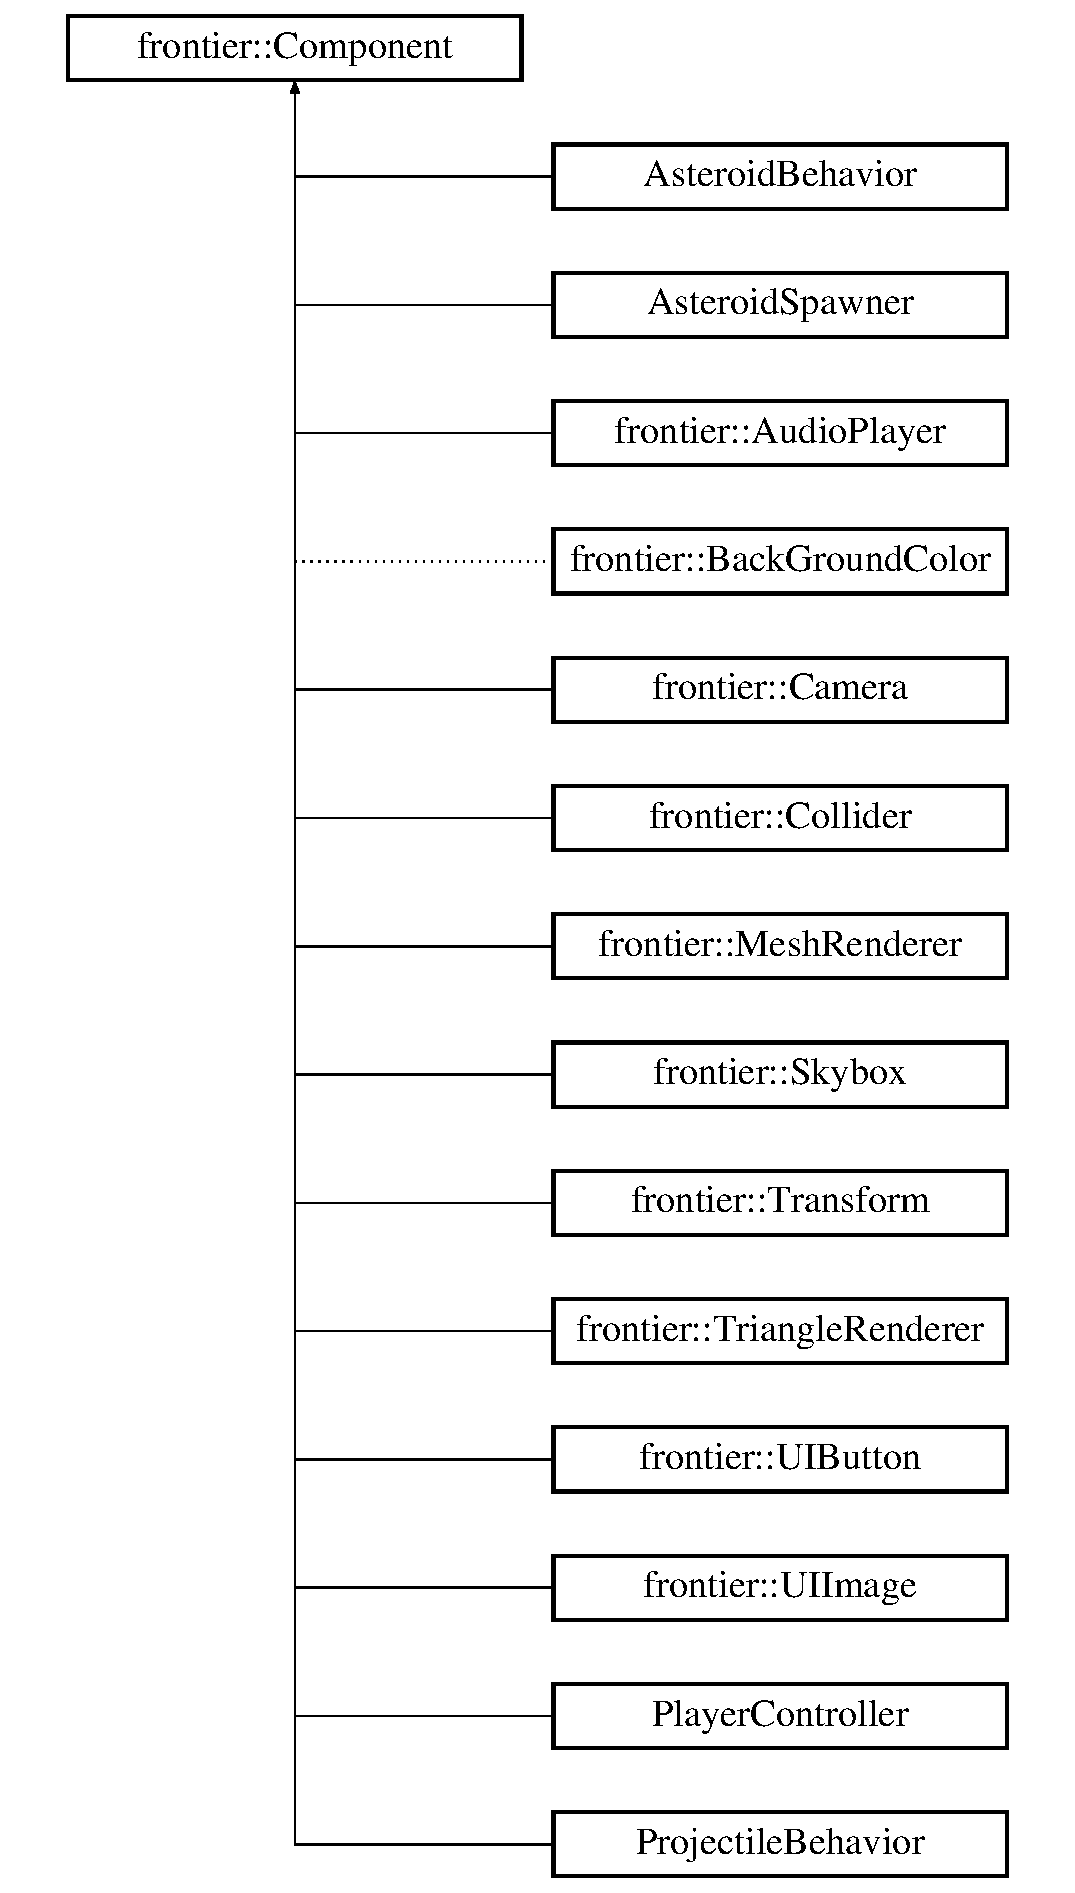
\includegraphics[height=12.000000cm]{classfrontier_1_1_component}
\end{center}
\end{figure}
\subsection*{Public Member Functions}
\begin{DoxyCompactItemize}
\item 
virtual void \hyperlink{classfrontier_1_1_component_af3da02905c4d79219d9b12f260a35ad1}{On\+Init} (std\+::weak\+\_\+ptr$<$ \hyperlink{classfrontier_1_1_entity}{Entity} $>$ \+\_\+parent)
\begin{DoxyCompactList}\small\item\em Initialises the component. Sets the pointer to the entity that this component is attached to. \end{DoxyCompactList}\item 
virtual void \hyperlink{classfrontier_1_1_component_a77fca7ba1960aafb9bc05905e300c79d}{On\+Activate} ()
\begin{DoxyCompactList}\small\item\em Called when an entity\textquotesingle{}s active state is changed from false to true. \end{DoxyCompactList}\item 
virtual void \hyperlink{classfrontier_1_1_component_ab920f9bc07ce051ebb5559c5a66508d1}{On\+Tick} ()
\begin{DoxyCompactList}\small\item\em Called every frame, use for data that needs to be calculated each frame. \end{DoxyCompactList}\item 
std\+::shared\+\_\+ptr$<$ \hyperlink{classfrontier_1_1_entity}{Entity} $>$ \hyperlink{classfrontier_1_1_component_a4d4193dbf06629b5e457fb8f7d460e49}{Get\+Entity} ()
\begin{DoxyCompactList}\small\item\em Returns the entity that this component is attached to. \end{DoxyCompactList}\item 
bool \hyperlink{classfrontier_1_1_component_a22a2ac83f030cd83415a51f584cf2d32}{Is\+Copyable} ()
\begin{DoxyCompactList}\small\item\em Returns if the class is copyable for a prefab. \end{DoxyCompactList}\end{DoxyCompactItemize}
\subsection*{Protected Member Functions}
\begin{DoxyCompactItemize}
\item 
std\+::shared\+\_\+ptr$<$ \hyperlink{classfrontier_1_1_core}{Core} $>$ \hyperlink{classfrontier_1_1_component_a0006685ddaadb379360f7f28294d3806}{Get\+Core} ()
\begin{DoxyCompactList}\small\item\em Returns a pointer to the core. \end{DoxyCompactList}\item 
std\+::shared\+\_\+ptr$<$ \hyperlink{classfrontier_1_1_input}{Input} $>$ \hyperlink{classfrontier_1_1_component_a25cc51fb97b0b4c5dad1401707d530ea}{Get\+Input} ()
\begin{DoxyCompactList}\small\item\em Returns a pointer to the input class. \end{DoxyCompactList}\item 
std\+::shared\+\_\+ptr$<$ \hyperlink{classfrontier_1_1_environment}{Environment} $>$ \hyperlink{classfrontier_1_1_component_a24846c0ac8d4d607aff483ed7ffdf5f8}{Get\+Environment} ()
\begin{DoxyCompactList}\small\item\em Returns a pointer to the environment class. \end{DoxyCompactList}\end{DoxyCompactItemize}
\subsection*{Protected Attributes}
\begin{DoxyCompactItemize}
\item 
bool \hyperlink{classfrontier_1_1_component_ad15af6da45dff3b37abb83bd5697fd87}{m\+\_\+copyable} = false
\begin{DoxyCompactList}\small\item\em Determines if a component has a copy constructor. \end{DoxyCompactList}\end{DoxyCompactItemize}


\subsection{Detailed Description}
Base component class, use for inheritance to other classes only. Useless on its own. 

\subsection{Member Function Documentation}
\mbox{\Hypertarget{classfrontier_1_1_component_a0006685ddaadb379360f7f28294d3806}\label{classfrontier_1_1_component_a0006685ddaadb379360f7f28294d3806}} 
\index{frontier\+::\+Component@{frontier\+::\+Component}!Get\+Core@{Get\+Core}}
\index{Get\+Core@{Get\+Core}!frontier\+::\+Component@{frontier\+::\+Component}}
\subsubsection{\texorpdfstring{Get\+Core()}{GetCore()}}
{\footnotesize\ttfamily std\+::shared\+\_\+ptr$<$ \hyperlink{classfrontier_1_1_core}{Core} $>$ frontier\+::\+Component\+::\+Get\+Core (\begin{DoxyParamCaption}{ }\end{DoxyParamCaption})\hspace{0.3cm}{\ttfamily [protected]}}



Returns a pointer to the core. 

\mbox{\Hypertarget{classfrontier_1_1_component_a4d4193dbf06629b5e457fb8f7d460e49}\label{classfrontier_1_1_component_a4d4193dbf06629b5e457fb8f7d460e49}} 
\index{frontier\+::\+Component@{frontier\+::\+Component}!Get\+Entity@{Get\+Entity}}
\index{Get\+Entity@{Get\+Entity}!frontier\+::\+Component@{frontier\+::\+Component}}
\subsubsection{\texorpdfstring{Get\+Entity()}{GetEntity()}}
{\footnotesize\ttfamily std\+::shared\+\_\+ptr$<$ \hyperlink{classfrontier_1_1_entity}{Entity} $>$ frontier\+::\+Component\+::\+Get\+Entity (\begin{DoxyParamCaption}{ }\end{DoxyParamCaption})}



Returns the entity that this component is attached to. 

\mbox{\Hypertarget{classfrontier_1_1_component_a24846c0ac8d4d607aff483ed7ffdf5f8}\label{classfrontier_1_1_component_a24846c0ac8d4d607aff483ed7ffdf5f8}} 
\index{frontier\+::\+Component@{frontier\+::\+Component}!Get\+Environment@{Get\+Environment}}
\index{Get\+Environment@{Get\+Environment}!frontier\+::\+Component@{frontier\+::\+Component}}
\subsubsection{\texorpdfstring{Get\+Environment()}{GetEnvironment()}}
{\footnotesize\ttfamily std\+::shared\+\_\+ptr$<$ \hyperlink{classfrontier_1_1_environment}{Environment} $>$ frontier\+::\+Component\+::\+Get\+Environment (\begin{DoxyParamCaption}{ }\end{DoxyParamCaption})\hspace{0.3cm}{\ttfamily [protected]}}



Returns a pointer to the environment class. 

\mbox{\Hypertarget{classfrontier_1_1_component_a25cc51fb97b0b4c5dad1401707d530ea}\label{classfrontier_1_1_component_a25cc51fb97b0b4c5dad1401707d530ea}} 
\index{frontier\+::\+Component@{frontier\+::\+Component}!Get\+Input@{Get\+Input}}
\index{Get\+Input@{Get\+Input}!frontier\+::\+Component@{frontier\+::\+Component}}
\subsubsection{\texorpdfstring{Get\+Input()}{GetInput()}}
{\footnotesize\ttfamily std\+::shared\+\_\+ptr$<$ \hyperlink{classfrontier_1_1_input}{Input} $>$ frontier\+::\+Component\+::\+Get\+Input (\begin{DoxyParamCaption}{ }\end{DoxyParamCaption})\hspace{0.3cm}{\ttfamily [protected]}}



Returns a pointer to the input class. 

\mbox{\Hypertarget{classfrontier_1_1_component_a22a2ac83f030cd83415a51f584cf2d32}\label{classfrontier_1_1_component_a22a2ac83f030cd83415a51f584cf2d32}} 
\index{frontier\+::\+Component@{frontier\+::\+Component}!Is\+Copyable@{Is\+Copyable}}
\index{Is\+Copyable@{Is\+Copyable}!frontier\+::\+Component@{frontier\+::\+Component}}
\subsubsection{\texorpdfstring{Is\+Copyable()}{IsCopyable()}}
{\footnotesize\ttfamily bool frontier\+::\+Component\+::\+Is\+Copyable (\begin{DoxyParamCaption}{ }\end{DoxyParamCaption})}



Returns if the class is copyable for a prefab. 

\mbox{\Hypertarget{classfrontier_1_1_component_a77fca7ba1960aafb9bc05905e300c79d}\label{classfrontier_1_1_component_a77fca7ba1960aafb9bc05905e300c79d}} 
\index{frontier\+::\+Component@{frontier\+::\+Component}!On\+Activate@{On\+Activate}}
\index{On\+Activate@{On\+Activate}!frontier\+::\+Component@{frontier\+::\+Component}}
\subsubsection{\texorpdfstring{On\+Activate()}{OnActivate()}}
{\footnotesize\ttfamily void frontier\+::\+Component\+::\+On\+Activate (\begin{DoxyParamCaption}{ }\end{DoxyParamCaption})\hspace{0.3cm}{\ttfamily [virtual]}}



Called when an entity\textquotesingle{}s active state is changed from false to true. 



Reimplemented in \hyperlink{class_asteroid_behavior_a7c4f344a9461d1296d4dcfcd51ed3bbc}{Asteroid\+Behavior}, and \hyperlink{class_projectile_behavior_aa01c813e541f6069d7ca9c69848ca0a6}{Projectile\+Behavior}.

\mbox{\Hypertarget{classfrontier_1_1_component_af3da02905c4d79219d9b12f260a35ad1}\label{classfrontier_1_1_component_af3da02905c4d79219d9b12f260a35ad1}} 
\index{frontier\+::\+Component@{frontier\+::\+Component}!On\+Init@{On\+Init}}
\index{On\+Init@{On\+Init}!frontier\+::\+Component@{frontier\+::\+Component}}
\subsubsection{\texorpdfstring{On\+Init()}{OnInit()}}
{\footnotesize\ttfamily void frontier\+::\+Component\+::\+On\+Init (\begin{DoxyParamCaption}\item[{std\+::weak\+\_\+ptr$<$ \hyperlink{classfrontier_1_1_entity}{Entity} $>$}]{\+\_\+parent }\end{DoxyParamCaption})\hspace{0.3cm}{\ttfamily [virtual]}}



Initialises the component. Sets the pointer to the entity that this component is attached to. 


\begin{DoxyParams}{Parameters}
{\em \+\_\+parent} & The entity that the component will be attached to. \\
\hline
\end{DoxyParams}


Reimplemented in \hyperlink{classfrontier_1_1_transform_a2d8181ec0003b04822124340fe7772c0}{frontier\+::\+Transform}, \hyperlink{classfrontier_1_1_u_i_image_ad862e7dd5bcd1c2847001f5e1b56c114}{frontier\+::\+U\+I\+Image}, \hyperlink{classfrontier_1_1_u_i_button_a1c4555865094fdd2dd9dd595740c05b0}{frontier\+::\+U\+I\+Button}, \hyperlink{class_asteroid_behavior_a79d9559f0d8e109e928acf7f8ff7acea}{Asteroid\+Behavior}, and \hyperlink{class_player_controller_a22c60d9e4464ee585f3592593f14bc50}{Player\+Controller}.

\mbox{\Hypertarget{classfrontier_1_1_component_ab920f9bc07ce051ebb5559c5a66508d1}\label{classfrontier_1_1_component_ab920f9bc07ce051ebb5559c5a66508d1}} 
\index{frontier\+::\+Component@{frontier\+::\+Component}!On\+Tick@{On\+Tick}}
\index{On\+Tick@{On\+Tick}!frontier\+::\+Component@{frontier\+::\+Component}}
\subsubsection{\texorpdfstring{On\+Tick()}{OnTick()}}
{\footnotesize\ttfamily void frontier\+::\+Component\+::\+On\+Tick (\begin{DoxyParamCaption}{ }\end{DoxyParamCaption})\hspace{0.3cm}{\ttfamily [virtual]}}



Called every frame, use for data that needs to be calculated each frame. 



Reimplemented in \hyperlink{classfrontier_1_1_collider_ac03782c94e8f7a2064ea1441cbd12c81}{frontier\+::\+Collider}, \hyperlink{classfrontier_1_1_mesh_renderer_acffde7174ddb009751e360df5d346922}{frontier\+::\+Mesh\+Renderer}, \hyperlink{classfrontier_1_1_u_i_image_a4e0d055c0add55fa5e63ae892ea59498}{frontier\+::\+U\+I\+Image}, \hyperlink{classfrontier_1_1_u_i_button_a8eda4323e4d0c2cd2c6a4639f39a1a09}{frontier\+::\+U\+I\+Button}, \hyperlink{classfrontier_1_1_skybox_a38b2ec1a28314c901f4388745d8f0471}{frontier\+::\+Skybox}, \hyperlink{class_asteroid_spawner_acd2744a9a1ac8f13ac28220b33b9f750}{Asteroid\+Spawner}, \hyperlink{class_asteroid_behavior_a3c1287599e132b49be851d9eeec6380e}{Asteroid\+Behavior}, \hyperlink{class_projectile_behavior_a7756651ba998e7f3c0abcafcf25796ae}{Projectile\+Behavior}, and \hyperlink{class_player_controller_a5641058df338563ff6bb6bce7645ef7b}{Player\+Controller}.



\subsection{Member Data Documentation}
\mbox{\Hypertarget{classfrontier_1_1_component_ad15af6da45dff3b37abb83bd5697fd87}\label{classfrontier_1_1_component_ad15af6da45dff3b37abb83bd5697fd87}} 
\index{frontier\+::\+Component@{frontier\+::\+Component}!m\+\_\+copyable@{m\+\_\+copyable}}
\index{m\+\_\+copyable@{m\+\_\+copyable}!frontier\+::\+Component@{frontier\+::\+Component}}
\subsubsection{\texorpdfstring{m\+\_\+copyable}{m\_copyable}}
{\footnotesize\ttfamily bool frontier\+::\+Component\+::m\+\_\+copyable = false\hspace{0.3cm}{\ttfamily [protected]}}



Determines if a component has a copy constructor. 



The documentation for this class was generated from the following files\+:\begin{DoxyCompactItemize}
\item 
src/myengine/\hyperlink{_component_8h}{Component.\+h}\item 
src/myengine/\hyperlink{_component_8cpp}{Component.\+cpp}\end{DoxyCompactItemize}

\hypertarget{classfrontier_1_1_core}{}\section{frontier\+:\+:Core Class Reference}
\label{classfrontier_1_1_core}\index{frontier\+::\+Core@{frontier\+::\+Core}}


The main core of the engine. This is where all entities, prefabs and resources get created.  




{\ttfamily \#include $<$Core.\+h$>$}

Inheritance diagram for frontier\+:\+:Core\+:\begin{figure}[H]
\begin{center}
\leavevmode
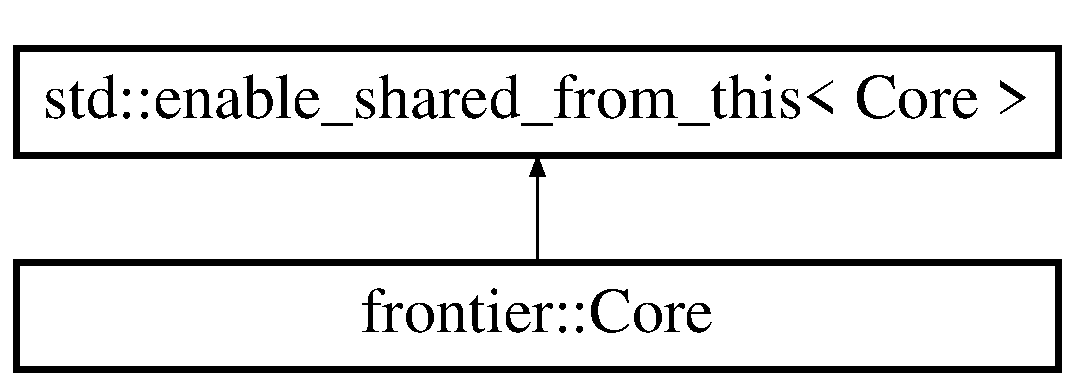
\includegraphics[height=2.000000cm]{classfrontier_1_1_core}
\end{center}
\end{figure}
\subsection*{Public Member Functions}
\begin{DoxyCompactItemize}
\item 
\hyperlink{classfrontier_1_1_core_a4d5ae078d34758c54c517bede518e2e4}{$\sim$\+Core} ()
\begin{DoxyCompactList}\small\item\em Destructor for the core, removes all entities from stored vector list. \end{DoxyCompactList}\item 
void \hyperlink{classfrontier_1_1_core_a4faf575f20b1d83732da965476275371}{Init} (std\+::weak\+\_\+ptr$<$ \hyperlink{classfrontier_1_1_core}{Core} $>$ \+\_\+self, int \+\_\+width=800, int \+\_\+height=600)
\begin{DoxyCompactList}\small\item\em Initialisation for the core, sets up Open\+GL, S\+DL, Open\+AL and all other classes needed by the core. \end{DoxyCompactList}\item 
void \hyperlink{classfrontier_1_1_core_a184b56e6f852d9670168111e5e1a1bc2}{Start} ()
\begin{DoxyCompactList}\small\item\em Starts the game, this starts the game loop and makes everything run. Do not call this until everything has been set up. \end{DoxyCompactList}\item 
void \hyperlink{classfrontier_1_1_core_af73d19f41d8316a7e0a6e11137201ed9}{Stop} ()
\begin{DoxyCompactList}\small\item\em Stops the game, closes down any classes that need to be de-\/initialised. \end{DoxyCompactList}\item 
std\+::shared\+\_\+ptr$<$ \hyperlink{classfrontier_1_1_entity}{Entity} $>$ \hyperlink{classfrontier_1_1_core_a6e7da5742a26a76b46a6f02aa079929c}{Add\+Entity} (glm\+::vec3 \+\_\+position=glm\+::vec3(0.\+0f, 0.\+0f, 0.\+0f), glm\+::vec3 \+\_\+rotation=glm\+::vec3(0.\+0f, 0.\+0f, 0.\+0f), glm\+::vec3 \+\_\+scale=glm\+::vec3(1.\+0f, 1.\+0f, 1.\+0f))
\begin{DoxyCompactList}\small\item\em Adds an entity and returns a pointer to it. \end{DoxyCompactList}\item 
std\+::shared\+\_\+ptr$<$ \hyperlink{classfrontier_1_1_entity}{Entity} $>$ \hyperlink{classfrontier_1_1_core_a87217c1aa2c91e76d006c0f3dfeba309}{Add\+Entity} (std\+::shared\+\_\+ptr$<$ \hyperlink{classfrontier_1_1_prefab}{Prefab} $>$ \+\_\+prefab, glm\+::vec3 \+\_\+position=glm\+::vec3(0.\+0f, 0.\+0f, 0.\+0f), glm\+::vec3 \+\_\+rotation=glm\+::vec3(0.\+0f, 0.\+0f, 0.\+0f), glm\+::vec3 \+\_\+scale=glm\+::vec3(1.\+0f, 1.\+0f, 1.\+0f))
\begin{DoxyCompactList}\small\item\em Adds an entity using a prefab and returns a pointer to it. \end{DoxyCompactList}\item 
std\+::shared\+\_\+ptr$<$ \hyperlink{classfrontier_1_1_entity}{Entity} $>$ \hyperlink{classfrontier_1_1_core_afa83f3a99653170b1f6f6e5661a2a5f5}{Add\+U\+I\+Element} (glm\+::vec2 \+\_\+position=glm\+::vec2(0.\+0f, 0.\+0f), float \+\_\+rotation=0.\+0f, glm\+::vec3 \+\_\+scale=glm\+::vec3(1.\+0f, 1.\+0f, 1.\+0f))
\begin{DoxyCompactList}\small\item\em Adds a UI element entity, a UI element entity has it\textquotesingle{}s on tick function prioritised over non-\/ui entities. \end{DoxyCompactList}\item 
std\+::shared\+\_\+ptr$<$ \hyperlink{classfrontier_1_1_prefab}{Prefab} $>$ \hyperlink{classfrontier_1_1_core_a5be4be857929a89eee24411504038c72}{Add\+Prefab} ()
\begin{DoxyCompactList}\small\item\em Adds a prefab and returns a pointer to it. \end{DoxyCompactList}\item 
std\+::shared\+\_\+ptr$<$ \hyperlink{classfrontier_1_1_pooler}{Pooler} $>$ \hyperlink{classfrontier_1_1_core_a75859114b2e1acae74a7ec0ab4175c14}{Add\+Pooler} (std\+::string \+\_\+id, std\+::shared\+\_\+ptr$<$ \hyperlink{classfrontier_1_1_prefab}{Prefab} $>$ \+\_\+prefab, int \+\_\+initial\+Pool\+Size)
\begin{DoxyCompactList}\small\item\em Adds a pooler for use with a lot of instances of entities. \end{DoxyCompactList}\item 
std\+::shared\+\_\+ptr$<$ \hyperlink{classfrontier_1_1_pooler}{Pooler} $>$ \hyperlink{classfrontier_1_1_core_a1ebe697a4700dfc8f3ba4749aa9bd854}{Get\+Pooler} (std\+::string \+\_\+pool\+ID)
\begin{DoxyCompactList}\small\item\em Returns a pooler with the given ID. \end{DoxyCompactList}\item 
std\+::shared\+\_\+ptr$<$ \hyperlink{classfrontier_1_1_environment}{Environment} $>$ \hyperlink{classfrontier_1_1_core_a38ded93a4688d58e6e3ef2cdd7694a7a}{Get\+Environment} ()
\begin{DoxyCompactList}\small\item\em Returns the instance of the environment class. \end{DoxyCompactList}\item 
std\+::shared\+\_\+ptr$<$ \hyperlink{classfrontier_1_1_input}{Input} $>$ \hyperlink{classfrontier_1_1_core_a4098db42dc9ad76fb1b7f579cea45bd2}{Get\+Input} ()
\begin{DoxyCompactList}\small\item\em Returns the instance of the input class. \end{DoxyCompactList}\item 
std\+::shared\+\_\+ptr$<$ \hyperlink{classfrontier_1_1_resources}{Resources} $>$ \hyperlink{classfrontier_1_1_core_af05275451ce494dd3df46ed97b6f643a}{Get\+Resources} ()
\begin{DoxyCompactList}\small\item\em Returns the instance of the resources class. \end{DoxyCompactList}\item 
void \hyperlink{classfrontier_1_1_core_a92669a2d7754db9bcf3ff600f54952ae}{Set\+Self} (std\+::weak\+\_\+ptr$<$ \hyperlink{classfrontier_1_1_core}{Core} $>$ \+\_\+self\+Ptr)
\begin{DoxyCompactList}\small\item\em Sets the self pointer to be used in entity intialisation. \end{DoxyCompactList}\item 
int \hyperlink{classfrontier_1_1_core_a92d5a3acd90860e5cdbbe0030a711b22}{Get\+Width} ()
\begin{DoxyCompactList}\small\item\em Returns the width of the screen. \end{DoxyCompactList}\item 
int \hyperlink{classfrontier_1_1_core_a30d2a3deec19493bba0e3a7a9d04a11b}{Get\+Height} ()
\begin{DoxyCompactList}\small\item\em Returns the height of the screen. \end{DoxyCompactList}\item 
std\+::shared\+\_\+ptr$<$ \hyperlink{classfrontier_1_1_camera}{Camera} $>$ \hyperlink{classfrontier_1_1_core_a78b3939fe11820a0c041c984a25107b3}{Get\+Main\+Camera} ()
\begin{DoxyCompactList}\small\item\em Returns a pointer to the current main camera. \end{DoxyCompactList}\item 
void \hyperlink{classfrontier_1_1_core_a601db94399406b9091a76972d948dc6b}{Set\+Main\+Camera} (std\+::shared\+\_\+ptr$<$ \hyperlink{classfrontier_1_1_camera}{Camera} $>$ \+\_\+main\+Camera\+To\+Set)
\begin{DoxyCompactList}\small\item\em Sets a new main camera and unsets the previous one. \end{DoxyCompactList}\item 
void \hyperlink{classfrontier_1_1_core_a10aea6f8fa81b54595845386c3d3f6cf}{Deactivate\+All\+Instances\+In\+Pools} ()
\begin{DoxyCompactList}\small\item\em Sets all entities in pools to inactive. \end{DoxyCompactList}\item 
std\+::shared\+\_\+ptr$<$ \hyperlink{classfrontier_1_1_shader}{Shader} $>$ \hyperlink{classfrontier_1_1_core_a5c92add403b305f061f691d9c21d63c0}{get\+Hitbox\+Shader} ()
\begin{DoxyCompactList}\small\item\em Returns a pointer to the default hitbox shader. \end{DoxyCompactList}\item 
std\+::shared\+\_\+ptr$<$ \hyperlink{classfrontier_1_1_shader}{Shader} $>$ \hyperlink{classfrontier_1_1_core_a0da8b576b0d812148924827da5c05a3d}{get\+Skybox\+Shader} ()
\begin{DoxyCompactList}\small\item\em Returns a pointer to the default skybox shader. \end{DoxyCompactList}\item 
std\+::shared\+\_\+ptr$<$ \hyperlink{classfrontier_1_1_shader}{Shader} $>$ \hyperlink{classfrontier_1_1_core_a6b61c169b75acd9a15bf3009bc838901}{get\+Untextured\+Ui\+Image\+Shader} ()
\begin{DoxyCompactList}\small\item\em Returns a pointer to the default untextured UI shader. \end{DoxyCompactList}\item 
std\+::shared\+\_\+ptr$<$ \hyperlink{classfrontier_1_1_shader}{Shader} $>$ \hyperlink{classfrontier_1_1_core_aac07a29176bd8056e004f7be8c919d3f}{get\+Textured\+Ui\+Image\+Shader} ()
\begin{DoxyCompactList}\small\item\em Returns a pointer to the default textured UI shader. \end{DoxyCompactList}\item 
void \hyperlink{classfrontier_1_1_core_a0d510b25cca36dddb10b562913ae24c7}{Add\+To\+Entities\+To\+Activate} (std\+::shared\+\_\+ptr$<$ \hyperlink{classfrontier_1_1_entity}{Entity} $>$ \+\_\+entity\+To\+Activate)
\begin{DoxyCompactList}\small\item\em Adds an entity to activation list so that it can be activated next frame. \end{DoxyCompactList}\item 
{\footnotesize template$<$typename T $>$ }\\std\+::vector$<$ std\+::weak\+\_\+ptr$<$ \hyperlink{classfrontier_1_1_entity}{Entity} $>$ $>$ \hyperlink{classfrontier_1_1_core_a8c42c287ec4a96ff3be194f92e82c367}{get\+Entities\+With\+Component} ()
\begin{DoxyCompactList}\small\item\em returns a vector with all entities with a specified component. \end{DoxyCompactList}\end{DoxyCompactItemize}


\subsection{Detailed Description}
The main core of the engine. This is where all entities, prefabs and resources get created. 

\subsection{Constructor \& Destructor Documentation}
\mbox{\Hypertarget{classfrontier_1_1_core_a4d5ae078d34758c54c517bede518e2e4}\label{classfrontier_1_1_core_a4d5ae078d34758c54c517bede518e2e4}} 
\index{frontier\+::\+Core@{frontier\+::\+Core}!````~Core@{$\sim$\+Core}}
\index{````~Core@{$\sim$\+Core}!frontier\+::\+Core@{frontier\+::\+Core}}
\subsubsection{\texorpdfstring{$\sim$\+Core()}{~Core()}}
{\footnotesize\ttfamily frontier\+::\+Core\+::$\sim$\+Core (\begin{DoxyParamCaption}{ }\end{DoxyParamCaption})}



Destructor for the core, removes all entities from stored vector list. 



\subsection{Member Function Documentation}
\mbox{\Hypertarget{classfrontier_1_1_core_a6e7da5742a26a76b46a6f02aa079929c}\label{classfrontier_1_1_core_a6e7da5742a26a76b46a6f02aa079929c}} 
\index{frontier\+::\+Core@{frontier\+::\+Core}!Add\+Entity@{Add\+Entity}}
\index{Add\+Entity@{Add\+Entity}!frontier\+::\+Core@{frontier\+::\+Core}}
\subsubsection{\texorpdfstring{Add\+Entity()}{AddEntity()}\hspace{0.1cm}{\footnotesize\ttfamily [1/2]}}
{\footnotesize\ttfamily std\+::shared\+\_\+ptr$<$ \hyperlink{classfrontier_1_1_entity}{Entity} $>$ frontier\+::\+Core\+::\+Add\+Entity (\begin{DoxyParamCaption}\item[{glm\+::vec3}]{\+\_\+position = {\ttfamily glm\+:\+:vec3(0.0f,~0.0f,~0.0f)},  }\item[{glm\+::vec3}]{\+\_\+rotation = {\ttfamily glm\+:\+:vec3(0.0f,~0.0f,~0.0f)},  }\item[{glm\+::vec3}]{\+\_\+scale = {\ttfamily glm\+:\+:vec3(1.0f,~1.0f,~1.0f)} }\end{DoxyParamCaption})}



Adds an entity and returns a pointer to it. 


\begin{DoxyParams}{Parameters}
{\em \+\_\+position} & The initial position of the entity (set to glm\+::vec3(0.\+0f, 0.\+0f, 0.\+0f) by default). \\
\hline
{\em \+\_\+rotation} & The initial rotation of the entity (set to glm\+::vec3(0.\+0f, 0.\+0f, 0.\+0f) by default). \\
\hline
{\em \+\_\+scale} & The initial scale of the entity (set to glm\+::vec3(1.\+0f, 1.\+0f, 1.\+0f) by default). \\
\hline
\end{DoxyParams}
\mbox{\Hypertarget{classfrontier_1_1_core_a87217c1aa2c91e76d006c0f3dfeba309}\label{classfrontier_1_1_core_a87217c1aa2c91e76d006c0f3dfeba309}} 
\index{frontier\+::\+Core@{frontier\+::\+Core}!Add\+Entity@{Add\+Entity}}
\index{Add\+Entity@{Add\+Entity}!frontier\+::\+Core@{frontier\+::\+Core}}
\subsubsection{\texorpdfstring{Add\+Entity()}{AddEntity()}\hspace{0.1cm}{\footnotesize\ttfamily [2/2]}}
{\footnotesize\ttfamily std\+::shared\+\_\+ptr$<$ \hyperlink{classfrontier_1_1_entity}{Entity} $>$ frontier\+::\+Core\+::\+Add\+Entity (\begin{DoxyParamCaption}\item[{std\+::shared\+\_\+ptr$<$ \hyperlink{classfrontier_1_1_prefab}{Prefab} $>$}]{\+\_\+prefab,  }\item[{glm\+::vec3}]{\+\_\+position = {\ttfamily glm\+:\+:vec3(0.0f,~0.0f,~0.0f)},  }\item[{glm\+::vec3}]{\+\_\+rotation = {\ttfamily glm\+:\+:vec3(0.0f,~0.0f,~0.0f)},  }\item[{glm\+::vec3}]{\+\_\+scale = {\ttfamily glm\+:\+:vec3(1.0f,~1.0f,~1.0f)} }\end{DoxyParamCaption})}



Adds an entity using a prefab and returns a pointer to it. 


\begin{DoxyParams}{Parameters}
{\em \+\_\+prefab} & The prefab which the entity will be copied from. \\
\hline
{\em \+\_\+position} & The initial position of the entity (set to glm\+::vec3(0.\+0f, 0.\+0f, 0.\+0f) by default). \\
\hline
{\em \+\_\+rotation} & The initial rotation of the entity (set to glm\+::vec3(0.\+0f, 0.\+0f, 0.\+0f) by default). \\
\hline
{\em \+\_\+scale} & The initial scale of the entity (set to glm\+::vec3(1.\+0f, 1.\+0f, 1.\+0f) by default). \\
\hline
\end{DoxyParams}
\mbox{\Hypertarget{classfrontier_1_1_core_a75859114b2e1acae74a7ec0ab4175c14}\label{classfrontier_1_1_core_a75859114b2e1acae74a7ec0ab4175c14}} 
\index{frontier\+::\+Core@{frontier\+::\+Core}!Add\+Pooler@{Add\+Pooler}}
\index{Add\+Pooler@{Add\+Pooler}!frontier\+::\+Core@{frontier\+::\+Core}}
\subsubsection{\texorpdfstring{Add\+Pooler()}{AddPooler()}}
{\footnotesize\ttfamily std\+::shared\+\_\+ptr$<$ \hyperlink{classfrontier_1_1_pooler}{Pooler} $>$ frontier\+::\+Core\+::\+Add\+Pooler (\begin{DoxyParamCaption}\item[{std\+::string}]{\+\_\+id,  }\item[{std\+::shared\+\_\+ptr$<$ \hyperlink{classfrontier_1_1_prefab}{Prefab} $>$}]{\+\_\+prefab,  }\item[{int}]{\+\_\+initial\+Pool\+Size }\end{DoxyParamCaption})}



Adds a pooler for use with a lot of instances of entities. 


\begin{DoxyParams}{Parameters}
{\em \+\_\+id} & string identifier for the pooler. \\
\hline
{\em \+\_\+prefab} & The prefab that entities will be created from. \\
\hline
{\em \+\_\+inital\+Pool\+Size} & The intial number of entities to be created. \\
\hline
\end{DoxyParams}
\mbox{\Hypertarget{classfrontier_1_1_core_a5be4be857929a89eee24411504038c72}\label{classfrontier_1_1_core_a5be4be857929a89eee24411504038c72}} 
\index{frontier\+::\+Core@{frontier\+::\+Core}!Add\+Prefab@{Add\+Prefab}}
\index{Add\+Prefab@{Add\+Prefab}!frontier\+::\+Core@{frontier\+::\+Core}}
\subsubsection{\texorpdfstring{Add\+Prefab()}{AddPrefab()}}
{\footnotesize\ttfamily std\+::shared\+\_\+ptr$<$ \hyperlink{classfrontier_1_1_prefab}{Prefab} $>$ frontier\+::\+Core\+::\+Add\+Prefab (\begin{DoxyParamCaption}{ }\end{DoxyParamCaption})}



Adds a prefab and returns a pointer to it. 

\mbox{\Hypertarget{classfrontier_1_1_core_a0d510b25cca36dddb10b562913ae24c7}\label{classfrontier_1_1_core_a0d510b25cca36dddb10b562913ae24c7}} 
\index{frontier\+::\+Core@{frontier\+::\+Core}!Add\+To\+Entities\+To\+Activate@{Add\+To\+Entities\+To\+Activate}}
\index{Add\+To\+Entities\+To\+Activate@{Add\+To\+Entities\+To\+Activate}!frontier\+::\+Core@{frontier\+::\+Core}}
\subsubsection{\texorpdfstring{Add\+To\+Entities\+To\+Activate()}{AddToEntitiesToActivate()}}
{\footnotesize\ttfamily void frontier\+::\+Core\+::\+Add\+To\+Entities\+To\+Activate (\begin{DoxyParamCaption}\item[{std\+::shared\+\_\+ptr$<$ \hyperlink{classfrontier_1_1_entity}{Entity} $>$}]{\+\_\+entity\+To\+Activate }\end{DoxyParamCaption})}



Adds an entity to activation list so that it can be activated next frame. 

\mbox{\Hypertarget{classfrontier_1_1_core_afa83f3a99653170b1f6f6e5661a2a5f5}\label{classfrontier_1_1_core_afa83f3a99653170b1f6f6e5661a2a5f5}} 
\index{frontier\+::\+Core@{frontier\+::\+Core}!Add\+U\+I\+Element@{Add\+U\+I\+Element}}
\index{Add\+U\+I\+Element@{Add\+U\+I\+Element}!frontier\+::\+Core@{frontier\+::\+Core}}
\subsubsection{\texorpdfstring{Add\+U\+I\+Element()}{AddUIElement()}}
{\footnotesize\ttfamily std\+::shared\+\_\+ptr$<$ \hyperlink{classfrontier_1_1_entity}{Entity} $>$ frontier\+::\+Core\+::\+Add\+U\+I\+Element (\begin{DoxyParamCaption}\item[{glm\+::vec2}]{\+\_\+position = {\ttfamily glm\+:\+:vec2(0.0f,~0.0f)},  }\item[{float}]{\+\_\+rotation = {\ttfamily 0.0f},  }\item[{glm\+::vec3}]{\+\_\+scale = {\ttfamily glm\+:\+:vec3(1.0f,~1.0f,~1.0f)} }\end{DoxyParamCaption})}



Adds a UI element entity, a UI element entity has it\textquotesingle{}s on tick function prioritised over non-\/ui entities. 


\begin{DoxyParams}{Parameters}
{\em \+\_\+position} & The initial position of the entity in screen space (set to glm\+::vec2(0.\+0f, 0.\+0f) by default). \\
\hline
{\em \+\_\+rotation} & The initial rotation of the entity (set to 0.\+0f by default). \\
\hline
{\em \+\_\+scale} & The initial scale of the entity (set to glm\+::vec3(1.\+0f, 1.\+0f, 1.\+0f) by default). \\
\hline
\end{DoxyParams}
\mbox{\Hypertarget{classfrontier_1_1_core_a10aea6f8fa81b54595845386c3d3f6cf}\label{classfrontier_1_1_core_a10aea6f8fa81b54595845386c3d3f6cf}} 
\index{frontier\+::\+Core@{frontier\+::\+Core}!Deactivate\+All\+Instances\+In\+Pools@{Deactivate\+All\+Instances\+In\+Pools}}
\index{Deactivate\+All\+Instances\+In\+Pools@{Deactivate\+All\+Instances\+In\+Pools}!frontier\+::\+Core@{frontier\+::\+Core}}
\subsubsection{\texorpdfstring{Deactivate\+All\+Instances\+In\+Pools()}{DeactivateAllInstancesInPools()}}
{\footnotesize\ttfamily void frontier\+::\+Core\+::\+Deactivate\+All\+Instances\+In\+Pools (\begin{DoxyParamCaption}{ }\end{DoxyParamCaption})}



Sets all entities in pools to inactive. 

\mbox{\Hypertarget{classfrontier_1_1_core_a8c42c287ec4a96ff3be194f92e82c367}\label{classfrontier_1_1_core_a8c42c287ec4a96ff3be194f92e82c367}} 
\index{frontier\+::\+Core@{frontier\+::\+Core}!get\+Entities\+With\+Component@{get\+Entities\+With\+Component}}
\index{get\+Entities\+With\+Component@{get\+Entities\+With\+Component}!frontier\+::\+Core@{frontier\+::\+Core}}
\subsubsection{\texorpdfstring{get\+Entities\+With\+Component()}{getEntitiesWithComponent()}}
{\footnotesize\ttfamily template$<$typename T $>$ \\
std\+::vector$<$std\+::weak\+\_\+ptr$<$\hyperlink{classfrontier_1_1_entity}{Entity}$>$ $>$ frontier\+::\+Core\+::get\+Entities\+With\+Component (\begin{DoxyParamCaption}{ }\end{DoxyParamCaption})\hspace{0.3cm}{\ttfamily [inline]}}



returns a vector with all entities with a specified component. 

\mbox{\Hypertarget{classfrontier_1_1_core_a38ded93a4688d58e6e3ef2cdd7694a7a}\label{classfrontier_1_1_core_a38ded93a4688d58e6e3ef2cdd7694a7a}} 
\index{frontier\+::\+Core@{frontier\+::\+Core}!Get\+Environment@{Get\+Environment}}
\index{Get\+Environment@{Get\+Environment}!frontier\+::\+Core@{frontier\+::\+Core}}
\subsubsection{\texorpdfstring{Get\+Environment()}{GetEnvironment()}}
{\footnotesize\ttfamily std\+::shared\+\_\+ptr$<$ \hyperlink{classfrontier_1_1_environment}{Environment} $>$ frontier\+::\+Core\+::\+Get\+Environment (\begin{DoxyParamCaption}{ }\end{DoxyParamCaption})}



Returns the instance of the environment class. 

\mbox{\Hypertarget{classfrontier_1_1_core_a30d2a3deec19493bba0e3a7a9d04a11b}\label{classfrontier_1_1_core_a30d2a3deec19493bba0e3a7a9d04a11b}} 
\index{frontier\+::\+Core@{frontier\+::\+Core}!Get\+Height@{Get\+Height}}
\index{Get\+Height@{Get\+Height}!frontier\+::\+Core@{frontier\+::\+Core}}
\subsubsection{\texorpdfstring{Get\+Height()}{GetHeight()}}
{\footnotesize\ttfamily int frontier\+::\+Core\+::\+Get\+Height (\begin{DoxyParamCaption}{ }\end{DoxyParamCaption})}



Returns the height of the screen. 

\mbox{\Hypertarget{classfrontier_1_1_core_a5c92add403b305f061f691d9c21d63c0}\label{classfrontier_1_1_core_a5c92add403b305f061f691d9c21d63c0}} 
\index{frontier\+::\+Core@{frontier\+::\+Core}!get\+Hitbox\+Shader@{get\+Hitbox\+Shader}}
\index{get\+Hitbox\+Shader@{get\+Hitbox\+Shader}!frontier\+::\+Core@{frontier\+::\+Core}}
\subsubsection{\texorpdfstring{get\+Hitbox\+Shader()}{getHitboxShader()}}
{\footnotesize\ttfamily std\+::shared\+\_\+ptr$<$ \hyperlink{classfrontier_1_1_shader}{Shader} $>$ frontier\+::\+Core\+::get\+Hitbox\+Shader (\begin{DoxyParamCaption}{ }\end{DoxyParamCaption})}



Returns a pointer to the default hitbox shader. 

\mbox{\Hypertarget{classfrontier_1_1_core_a4098db42dc9ad76fb1b7f579cea45bd2}\label{classfrontier_1_1_core_a4098db42dc9ad76fb1b7f579cea45bd2}} 
\index{frontier\+::\+Core@{frontier\+::\+Core}!Get\+Input@{Get\+Input}}
\index{Get\+Input@{Get\+Input}!frontier\+::\+Core@{frontier\+::\+Core}}
\subsubsection{\texorpdfstring{Get\+Input()}{GetInput()}}
{\footnotesize\ttfamily std\+::shared\+\_\+ptr$<$ \hyperlink{classfrontier_1_1_input}{Input} $>$ frontier\+::\+Core\+::\+Get\+Input (\begin{DoxyParamCaption}{ }\end{DoxyParamCaption})}



Returns the instance of the input class. 

\mbox{\Hypertarget{classfrontier_1_1_core_a78b3939fe11820a0c041c984a25107b3}\label{classfrontier_1_1_core_a78b3939fe11820a0c041c984a25107b3}} 
\index{frontier\+::\+Core@{frontier\+::\+Core}!Get\+Main\+Camera@{Get\+Main\+Camera}}
\index{Get\+Main\+Camera@{Get\+Main\+Camera}!frontier\+::\+Core@{frontier\+::\+Core}}
\subsubsection{\texorpdfstring{Get\+Main\+Camera()}{GetMainCamera()}}
{\footnotesize\ttfamily std\+::shared\+\_\+ptr$<$ \hyperlink{classfrontier_1_1_camera}{Camera} $>$ frontier\+::\+Core\+::\+Get\+Main\+Camera (\begin{DoxyParamCaption}{ }\end{DoxyParamCaption})}



Returns a pointer to the current main camera. 

\mbox{\Hypertarget{classfrontier_1_1_core_a1ebe697a4700dfc8f3ba4749aa9bd854}\label{classfrontier_1_1_core_a1ebe697a4700dfc8f3ba4749aa9bd854}} 
\index{frontier\+::\+Core@{frontier\+::\+Core}!Get\+Pooler@{Get\+Pooler}}
\index{Get\+Pooler@{Get\+Pooler}!frontier\+::\+Core@{frontier\+::\+Core}}
\subsubsection{\texorpdfstring{Get\+Pooler()}{GetPooler()}}
{\footnotesize\ttfamily std\+::shared\+\_\+ptr$<$ \hyperlink{classfrontier_1_1_pooler}{Pooler} $>$ frontier\+::\+Core\+::\+Get\+Pooler (\begin{DoxyParamCaption}\item[{std\+::string}]{\+\_\+pool\+ID }\end{DoxyParamCaption})}



Returns a pooler with the given ID. 


\begin{DoxyParams}{Parameters}
{\em \+\_\+pool\+ID} & the string identifier of the pool, must match the string created during initialisation of the pool (see add\+Pooler). \\
\hline
\end{DoxyParams}
\mbox{\Hypertarget{classfrontier_1_1_core_af05275451ce494dd3df46ed97b6f643a}\label{classfrontier_1_1_core_af05275451ce494dd3df46ed97b6f643a}} 
\index{frontier\+::\+Core@{frontier\+::\+Core}!Get\+Resources@{Get\+Resources}}
\index{Get\+Resources@{Get\+Resources}!frontier\+::\+Core@{frontier\+::\+Core}}
\subsubsection{\texorpdfstring{Get\+Resources()}{GetResources()}}
{\footnotesize\ttfamily std\+::shared\+\_\+ptr$<$ \hyperlink{classfrontier_1_1_resources}{Resources} $>$ frontier\+::\+Core\+::\+Get\+Resources (\begin{DoxyParamCaption}{ }\end{DoxyParamCaption})}



Returns the instance of the resources class. 

\mbox{\Hypertarget{classfrontier_1_1_core_a0da8b576b0d812148924827da5c05a3d}\label{classfrontier_1_1_core_a0da8b576b0d812148924827da5c05a3d}} 
\index{frontier\+::\+Core@{frontier\+::\+Core}!get\+Skybox\+Shader@{get\+Skybox\+Shader}}
\index{get\+Skybox\+Shader@{get\+Skybox\+Shader}!frontier\+::\+Core@{frontier\+::\+Core}}
\subsubsection{\texorpdfstring{get\+Skybox\+Shader()}{getSkyboxShader()}}
{\footnotesize\ttfamily std\+::shared\+\_\+ptr$<$ \hyperlink{classfrontier_1_1_shader}{Shader} $>$ frontier\+::\+Core\+::get\+Skybox\+Shader (\begin{DoxyParamCaption}{ }\end{DoxyParamCaption})}



Returns a pointer to the default skybox shader. 

\mbox{\Hypertarget{classfrontier_1_1_core_aac07a29176bd8056e004f7be8c919d3f}\label{classfrontier_1_1_core_aac07a29176bd8056e004f7be8c919d3f}} 
\index{frontier\+::\+Core@{frontier\+::\+Core}!get\+Textured\+Ui\+Image\+Shader@{get\+Textured\+Ui\+Image\+Shader}}
\index{get\+Textured\+Ui\+Image\+Shader@{get\+Textured\+Ui\+Image\+Shader}!frontier\+::\+Core@{frontier\+::\+Core}}
\subsubsection{\texorpdfstring{get\+Textured\+Ui\+Image\+Shader()}{getTexturedUiImageShader()}}
{\footnotesize\ttfamily std\+::shared\+\_\+ptr$<$ \hyperlink{classfrontier_1_1_shader}{Shader} $>$ frontier\+::\+Core\+::get\+Textured\+Ui\+Image\+Shader (\begin{DoxyParamCaption}{ }\end{DoxyParamCaption})}



Returns a pointer to the default textured UI shader. 

\mbox{\Hypertarget{classfrontier_1_1_core_a6b61c169b75acd9a15bf3009bc838901}\label{classfrontier_1_1_core_a6b61c169b75acd9a15bf3009bc838901}} 
\index{frontier\+::\+Core@{frontier\+::\+Core}!get\+Untextured\+Ui\+Image\+Shader@{get\+Untextured\+Ui\+Image\+Shader}}
\index{get\+Untextured\+Ui\+Image\+Shader@{get\+Untextured\+Ui\+Image\+Shader}!frontier\+::\+Core@{frontier\+::\+Core}}
\subsubsection{\texorpdfstring{get\+Untextured\+Ui\+Image\+Shader()}{getUntexturedUiImageShader()}}
{\footnotesize\ttfamily std\+::shared\+\_\+ptr$<$ \hyperlink{classfrontier_1_1_shader}{Shader} $>$ frontier\+::\+Core\+::get\+Untextured\+Ui\+Image\+Shader (\begin{DoxyParamCaption}{ }\end{DoxyParamCaption})}



Returns a pointer to the default untextured UI shader. 

\mbox{\Hypertarget{classfrontier_1_1_core_a92d5a3acd90860e5cdbbe0030a711b22}\label{classfrontier_1_1_core_a92d5a3acd90860e5cdbbe0030a711b22}} 
\index{frontier\+::\+Core@{frontier\+::\+Core}!Get\+Width@{Get\+Width}}
\index{Get\+Width@{Get\+Width}!frontier\+::\+Core@{frontier\+::\+Core}}
\subsubsection{\texorpdfstring{Get\+Width()}{GetWidth()}}
{\footnotesize\ttfamily int frontier\+::\+Core\+::\+Get\+Width (\begin{DoxyParamCaption}{ }\end{DoxyParamCaption})}



Returns the width of the screen. 

\mbox{\Hypertarget{classfrontier_1_1_core_a4faf575f20b1d83732da965476275371}\label{classfrontier_1_1_core_a4faf575f20b1d83732da965476275371}} 
\index{frontier\+::\+Core@{frontier\+::\+Core}!Init@{Init}}
\index{Init@{Init}!frontier\+::\+Core@{frontier\+::\+Core}}
\subsubsection{\texorpdfstring{Init()}{Init()}}
{\footnotesize\ttfamily void frontier\+::\+Core\+::\+Init (\begin{DoxyParamCaption}\item[{std\+::weak\+\_\+ptr$<$ \hyperlink{classfrontier_1_1_core}{Core} $>$}]{\+\_\+self,  }\item[{int}]{\+\_\+width = {\ttfamily 800},  }\item[{int}]{\+\_\+height = {\ttfamily 600} }\end{DoxyParamCaption})}



Initialisation for the core, sets up Open\+GL, S\+DL, Open\+AL and all other classes needed by the core. 


\begin{DoxyParams}{Parameters}
{\em \+\_\+self} & A pointer to the core, used to assign to entities. \\
\hline
{\em \+\_\+width} & The window width (set to 800 by default). \\
\hline
{\em \+\_\+height} & The window height (set to 600 by default). \\
\hline
\end{DoxyParams}
\mbox{\Hypertarget{classfrontier_1_1_core_a601db94399406b9091a76972d948dc6b}\label{classfrontier_1_1_core_a601db94399406b9091a76972d948dc6b}} 
\index{frontier\+::\+Core@{frontier\+::\+Core}!Set\+Main\+Camera@{Set\+Main\+Camera}}
\index{Set\+Main\+Camera@{Set\+Main\+Camera}!frontier\+::\+Core@{frontier\+::\+Core}}
\subsubsection{\texorpdfstring{Set\+Main\+Camera()}{SetMainCamera()}}
{\footnotesize\ttfamily void frontier\+::\+Core\+::\+Set\+Main\+Camera (\begin{DoxyParamCaption}\item[{std\+::shared\+\_\+ptr$<$ \hyperlink{classfrontier_1_1_camera}{Camera} $>$}]{\+\_\+main\+Camera\+To\+Set }\end{DoxyParamCaption})}



Sets a new main camera and unsets the previous one. 


\begin{DoxyParams}{Parameters}
{\em \+\_\+main\+Camera\+To\+Set} & A pointer to the new main camera. \\
\hline
\end{DoxyParams}
\mbox{\Hypertarget{classfrontier_1_1_core_a92669a2d7754db9bcf3ff600f54952ae}\label{classfrontier_1_1_core_a92669a2d7754db9bcf3ff600f54952ae}} 
\index{frontier\+::\+Core@{frontier\+::\+Core}!Set\+Self@{Set\+Self}}
\index{Set\+Self@{Set\+Self}!frontier\+::\+Core@{frontier\+::\+Core}}
\subsubsection{\texorpdfstring{Set\+Self()}{SetSelf()}}
{\footnotesize\ttfamily void frontier\+::\+Core\+::\+Set\+Self (\begin{DoxyParamCaption}\item[{std\+::weak\+\_\+ptr$<$ \hyperlink{classfrontier_1_1_core}{Core} $>$}]{\+\_\+self\+Ptr }\end{DoxyParamCaption})}



Sets the self pointer to be used in entity intialisation. 


\begin{DoxyParams}{Parameters}
{\em \+\_\+self} & A pointer to the core, used to assign to entities. \\
\hline
\end{DoxyParams}
\mbox{\Hypertarget{classfrontier_1_1_core_a184b56e6f852d9670168111e5e1a1bc2}\label{classfrontier_1_1_core_a184b56e6f852d9670168111e5e1a1bc2}} 
\index{frontier\+::\+Core@{frontier\+::\+Core}!Start@{Start}}
\index{Start@{Start}!frontier\+::\+Core@{frontier\+::\+Core}}
\subsubsection{\texorpdfstring{Start()}{Start()}}
{\footnotesize\ttfamily void frontier\+::\+Core\+::\+Start (\begin{DoxyParamCaption}{ }\end{DoxyParamCaption})}



Starts the game, this starts the game loop and makes everything run. Do not call this until everything has been set up. 

\mbox{\Hypertarget{classfrontier_1_1_core_af73d19f41d8316a7e0a6e11137201ed9}\label{classfrontier_1_1_core_af73d19f41d8316a7e0a6e11137201ed9}} 
\index{frontier\+::\+Core@{frontier\+::\+Core}!Stop@{Stop}}
\index{Stop@{Stop}!frontier\+::\+Core@{frontier\+::\+Core}}
\subsubsection{\texorpdfstring{Stop()}{Stop()}}
{\footnotesize\ttfamily void frontier\+::\+Core\+::\+Stop (\begin{DoxyParamCaption}{ }\end{DoxyParamCaption})}



Stops the game, closes down any classes that need to be de-\/initialised. 



The documentation for this class was generated from the following files\+:\begin{DoxyCompactItemize}
\item 
src/myengine/\hyperlink{_core_8h}{Core.\+h}\item 
src/myengine/\hyperlink{_core_8cpp}{Core.\+cpp}\end{DoxyCompactItemize}

\hypertarget{classfrontier_1_1_cubemap_texture}{}\section{frontier\+:\+:Cubemap\+Texture Class Reference}
\label{classfrontier_1_1_cubemap_texture}\index{frontier\+::\+Cubemap\+Texture@{frontier\+::\+Cubemap\+Texture}}


{\ttfamily \#include $<$Cubemap\+Texture.\+h$>$}

Inheritance diagram for frontier\+:\+:Cubemap\+Texture\+:\begin{figure}[H]
\begin{center}
\leavevmode
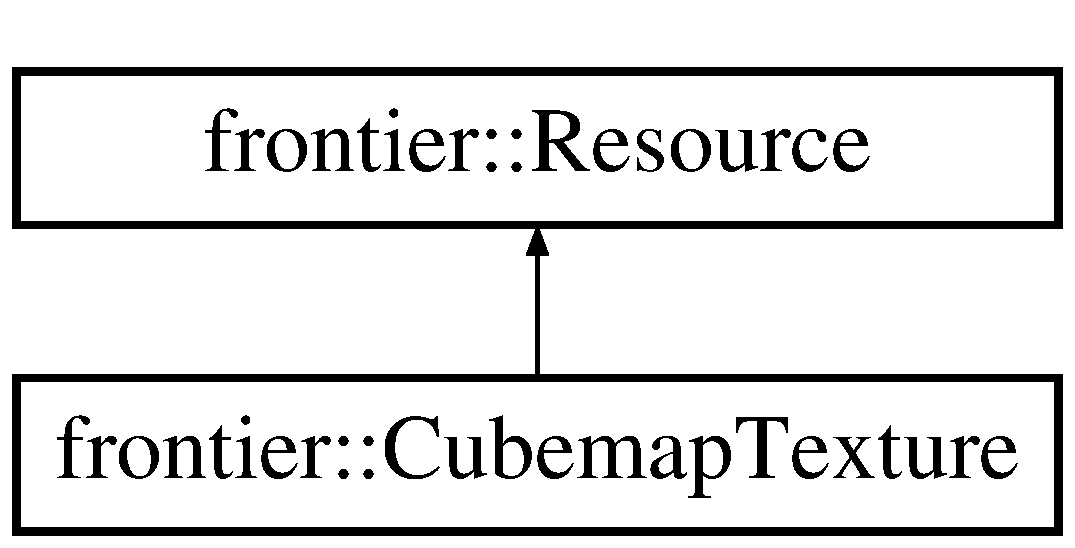
\includegraphics[height=2.000000cm]{classfrontier_1_1_cubemap_texture}
\end{center}
\end{figure}
\subsection*{Public Member Functions}
\begin{DoxyCompactItemize}
\item 
void \hyperlink{classfrontier_1_1_cubemap_texture_a479becfad071909e952d728cf6a8dacb}{Set\+Texture} (G\+Luint \+\_\+new\+ID, int \+\_\+\+Texture\+Location)
\item 
G\+Luint \hyperlink{classfrontier_1_1_cubemap_texture_a18b6320619de29cad6acd5fe50c42439}{Get\+Texture} ()
\item 
int \hyperlink{classfrontier_1_1_cubemap_texture_a091f7bd4e5233e5ce5f034ca17588387}{Get\+Texture\+Location} ()
\item 
void \hyperlink{classfrontier_1_1_cubemap_texture_aeddd79b5a1e438b532baf79be95452c7}{Bindtexture} ()
\end{DoxyCompactItemize}
\subsection*{Static Public Member Functions}
\begin{DoxyCompactItemize}
\item 
static std\+::shared\+\_\+ptr$<$ \hyperlink{classfrontier_1_1_cubemap_texture}{Cubemap\+Texture} $>$ \hyperlink{classfrontier_1_1_cubemap_texture_af9fdc5d920763022ccd3bacf90125075}{Create} (std\+::vector$<$ std\+::string $>$ \+\_\+paths, std\+::shared\+\_\+ptr$<$ \hyperlink{classfrontier_1_1_resources}{Resources} $>$ \+\_\+resources, int \+\_\+\+Texture\+Location)
\end{DoxyCompactItemize}
\subsection*{Additional Inherited Members}


\subsection{Member Function Documentation}
\mbox{\Hypertarget{classfrontier_1_1_cubemap_texture_aeddd79b5a1e438b532baf79be95452c7}\label{classfrontier_1_1_cubemap_texture_aeddd79b5a1e438b532baf79be95452c7}} 
\index{frontier\+::\+Cubemap\+Texture@{frontier\+::\+Cubemap\+Texture}!Bindtexture@{Bindtexture}}
\index{Bindtexture@{Bindtexture}!frontier\+::\+Cubemap\+Texture@{frontier\+::\+Cubemap\+Texture}}
\subsubsection{\texorpdfstring{Bindtexture()}{Bindtexture()}}
{\footnotesize\ttfamily void frontier\+::\+Cubemap\+Texture\+::\+Bindtexture (\begin{DoxyParamCaption}{ }\end{DoxyParamCaption})}

\mbox{\Hypertarget{classfrontier_1_1_cubemap_texture_af9fdc5d920763022ccd3bacf90125075}\label{classfrontier_1_1_cubemap_texture_af9fdc5d920763022ccd3bacf90125075}} 
\index{frontier\+::\+Cubemap\+Texture@{frontier\+::\+Cubemap\+Texture}!Create@{Create}}
\index{Create@{Create}!frontier\+::\+Cubemap\+Texture@{frontier\+::\+Cubemap\+Texture}}
\subsubsection{\texorpdfstring{Create()}{Create()}}
{\footnotesize\ttfamily std\+::shared\+\_\+ptr$<$ \hyperlink{classfrontier_1_1_cubemap_texture}{Cubemap\+Texture} $>$ frontier\+::\+Cubemap\+Texture\+::\+Create (\begin{DoxyParamCaption}\item[{std\+::vector$<$ std\+::string $>$}]{\+\_\+paths,  }\item[{std\+::shared\+\_\+ptr$<$ \hyperlink{classfrontier_1_1_resources}{Resources} $>$}]{\+\_\+resources,  }\item[{int}]{\+\_\+\+Texture\+Location }\end{DoxyParamCaption})\hspace{0.3cm}{\ttfamily [static]}}

\mbox{\Hypertarget{classfrontier_1_1_cubemap_texture_a18b6320619de29cad6acd5fe50c42439}\label{classfrontier_1_1_cubemap_texture_a18b6320619de29cad6acd5fe50c42439}} 
\index{frontier\+::\+Cubemap\+Texture@{frontier\+::\+Cubemap\+Texture}!Get\+Texture@{Get\+Texture}}
\index{Get\+Texture@{Get\+Texture}!frontier\+::\+Cubemap\+Texture@{frontier\+::\+Cubemap\+Texture}}
\subsubsection{\texorpdfstring{Get\+Texture()}{GetTexture()}}
{\footnotesize\ttfamily G\+Luint frontier\+::\+Cubemap\+Texture\+::\+Get\+Texture (\begin{DoxyParamCaption}{ }\end{DoxyParamCaption})}

\mbox{\Hypertarget{classfrontier_1_1_cubemap_texture_a091f7bd4e5233e5ce5f034ca17588387}\label{classfrontier_1_1_cubemap_texture_a091f7bd4e5233e5ce5f034ca17588387}} 
\index{frontier\+::\+Cubemap\+Texture@{frontier\+::\+Cubemap\+Texture}!Get\+Texture\+Location@{Get\+Texture\+Location}}
\index{Get\+Texture\+Location@{Get\+Texture\+Location}!frontier\+::\+Cubemap\+Texture@{frontier\+::\+Cubemap\+Texture}}
\subsubsection{\texorpdfstring{Get\+Texture\+Location()}{GetTextureLocation()}}
{\footnotesize\ttfamily int frontier\+::\+Cubemap\+Texture\+::\+Get\+Texture\+Location (\begin{DoxyParamCaption}{ }\end{DoxyParamCaption})}

\mbox{\Hypertarget{classfrontier_1_1_cubemap_texture_a479becfad071909e952d728cf6a8dacb}\label{classfrontier_1_1_cubemap_texture_a479becfad071909e952d728cf6a8dacb}} 
\index{frontier\+::\+Cubemap\+Texture@{frontier\+::\+Cubemap\+Texture}!Set\+Texture@{Set\+Texture}}
\index{Set\+Texture@{Set\+Texture}!frontier\+::\+Cubemap\+Texture@{frontier\+::\+Cubemap\+Texture}}
\subsubsection{\texorpdfstring{Set\+Texture()}{SetTexture()}}
{\footnotesize\ttfamily void frontier\+::\+Cubemap\+Texture\+::\+Set\+Texture (\begin{DoxyParamCaption}\item[{G\+Luint}]{\+\_\+new\+ID,  }\item[{int}]{\+\_\+\+Texture\+Location }\end{DoxyParamCaption})}



The documentation for this class was generated from the following files\+:\begin{DoxyCompactItemize}
\item 
src/myengine/\hyperlink{_cubemap_texture_8h}{Cubemap\+Texture.\+h}\item 
src/myengine/\hyperlink{_cubemap_texture_8cpp}{Cubemap\+Texture.\+cpp}\end{DoxyCompactItemize}

\hypertarget{classfrontier_1_1_entity}{}\section{frontier\+:\+:Entity Class Reference}
\label{classfrontier_1_1_entity}\index{frontier\+::\+Entity@{frontier\+::\+Entity}}


{\ttfamily \#include $<$Entity.\+h$>$}

Inheritance diagram for frontier\+:\+:Entity\+:\begin{figure}[H]
\begin{center}
\leavevmode
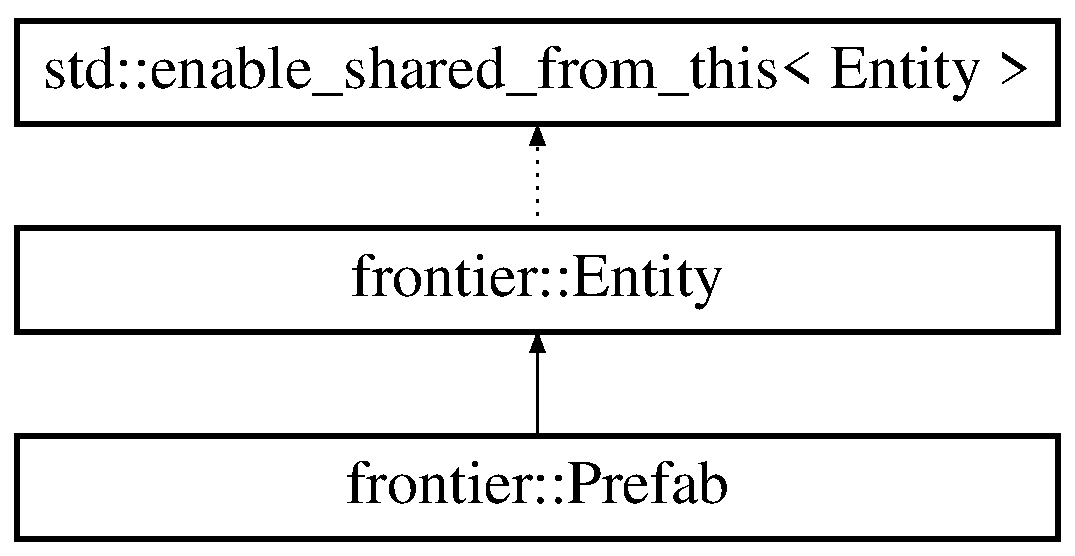
\includegraphics[height=3.000000cm]{classfrontier_1_1_entity}
\end{center}
\end{figure}
\subsection*{Public Member Functions}
\begin{DoxyCompactItemize}
\item 
\hyperlink{classfrontier_1_1_entity_a1d3f7c7fd0e6f01fa609e06fe76c8791}{Entity} ()
\item 
\hyperlink{classfrontier_1_1_entity_a56e4bc3a132b605bd8432259d8209808}{$\sim$\+Entity} ()
\item 
virtual void \hyperlink{classfrontier_1_1_entity_a9a37ec4188e73c190471a5de2db21c77}{init} (std\+::weak\+\_\+ptr$<$ \hyperlink{classfrontier_1_1_core}{Core} $>$ \+\_\+core\+Ptr)
\item 
void \hyperlink{classfrontier_1_1_entity_a8dd740cd4134ddab40663239527959e1}{init} (std\+::weak\+\_\+ptr$<$ \hyperlink{classfrontier_1_1_core}{Core} $>$ \+\_\+core\+Ptr, glm\+::vec3 \+\_\+position=glm\+::vec3(0.\+0f, 0.\+0f, 0.\+0f), glm\+::vec3 \+\_\+rotation=glm\+::vec3(0.\+0f, 0.\+0f, 0.\+0f), glm\+::vec3 \+\_\+scale=glm\+::vec3(1.\+0f, 1.\+0f, 1.\+0f))
\item 
void \hyperlink{classfrontier_1_1_entity_aba15243f8a661c4c9248e405fd869894}{init} (std\+::weak\+\_\+ptr$<$ \hyperlink{classfrontier_1_1_core}{Core} $>$ \+\_\+core\+Ptr, std\+::shared\+\_\+ptr$<$ \hyperlink{classfrontier_1_1_prefab}{Prefab} $>$ \+\_\+prefab, glm\+::vec3 \+\_\+position=glm\+::vec3(0.\+0f, 0.\+0f, 0.\+0f), glm\+::vec3 \+\_\+rotation=glm\+::vec3(0.\+0f, 0.\+0f, 0.\+0f), glm\+::vec3 \+\_\+scale=glm\+::vec3(1.\+0f, 1.\+0f, 1.\+0f))
\item 
std\+::shared\+\_\+ptr$<$ \hyperlink{classfrontier_1_1_core}{Core} $>$ \hyperlink{classfrontier_1_1_entity_a16f971a959ad628436e92368c342e2a2}{get\+Core} ()
\item 
void \hyperlink{classfrontier_1_1_entity_a99e123fc3c5fae5de4451fa5ea30d998}{tick} ()
\item 
void \hyperlink{classfrontier_1_1_entity_a35704148ee2160386445e9aaed3cbc78}{set\+Self} (std\+::weak\+\_\+ptr$<$ \hyperlink{classfrontier_1_1_entity}{Entity} $>$ \+\_\+self\+Ptr)
\item 
void \hyperlink{classfrontier_1_1_entity_a14b8bf3af26752cdd0240a9f48d411e1}{set\+Active} (bool active)
\item 
void \hyperlink{classfrontier_1_1_entity_a3a5eba11cf4dacc3de15ef460ee9d7de}{set\+Activating} (bool activating)
\item 
bool \hyperlink{classfrontier_1_1_entity_a1b19a21c357e557a3c12b6257d21ff09}{is\+Active} ()
\item 
bool \hyperlink{classfrontier_1_1_entity_a4de39f3a34645051d7d223b3f744761c}{is\+Activating} ()
\item 
{\footnotesize template$<$typename T $>$ }\\std\+::shared\+\_\+ptr$<$ T $>$ \hyperlink{classfrontier_1_1_entity_a7f78d98f8636d2db6fd9f6c6259f35cd}{add\+Component} ()
\item 
{\footnotesize template$<$typename T $>$ }\\std\+::shared\+\_\+ptr$<$ T $>$ \hyperlink{classfrontier_1_1_entity_a7e8950fc46a87fca465a94f66ac40494}{add\+Copy\+Of\+Component} (std\+::weak\+\_\+ptr$<$ T $>$ \+\_\+original)
\item 
{\footnotesize template$<$typename T , typename A $>$ }\\std\+::shared\+\_\+ptr$<$ T $>$ \hyperlink{classfrontier_1_1_entity_ab47b8543ddd540ce1ffb37c42f1d26fd}{add\+Component} (A \+\_\+a)
\item 
{\footnotesize template$<$typename T , typename A , typename B $>$ }\\std\+::shared\+\_\+ptr$<$ T $>$ \hyperlink{classfrontier_1_1_entity_a7b52a24fa9ecfe390bf0353ce9f87432}{add\+Component} (A \+\_\+a, B \+\_\+b)
\item 
{\footnotesize template$<$typename T , typename A , typename B , typename C $>$ }\\std\+::shared\+\_\+ptr$<$ T $>$ \hyperlink{classfrontier_1_1_entity_a0e27fe11f4f655d6ba1a63a5594d4efb}{add\+Component} (A \+\_\+a, B \+\_\+b, C \+\_\+c)
\item 
{\footnotesize template$<$typename T , typename A , typename B , typename C , typename D $>$ }\\std\+::shared\+\_\+ptr$<$ T $>$ \hyperlink{classfrontier_1_1_entity_a0a77572b04da8df53eea3aab783df9c7}{add\+Component} (A \+\_\+a, B \+\_\+b, C \+\_\+c, D \+\_\+d)
\item 
{\footnotesize template$<$typename T $>$ }\\std\+::shared\+\_\+ptr$<$ T $>$ \hyperlink{classfrontier_1_1_entity_a7657bce9cd7f405f69e59c61a69adf86}{get\+Component} ()
\item 
{\footnotesize template$<$typename T $>$ }\\bool \hyperlink{classfrontier_1_1_entity_a52e5f9cb6d6f8fddef34f58b7cc5daa8}{has\+Component} ()
\end{DoxyCompactItemize}
\subsection*{Protected Attributes}
\begin{DoxyCompactItemize}
\item 
std\+::weak\+\_\+ptr$<$ \hyperlink{classfrontier_1_1_core}{Core} $>$ \hyperlink{classfrontier_1_1_entity_aa6157be575485f3a37f11e57b5c8898e}{\+\_\+core}
\item 
std\+::weak\+\_\+ptr$<$ \hyperlink{classfrontier_1_1_entity}{Entity} $>$ \hyperlink{classfrontier_1_1_entity_a29a54e9eb639ffa8ac51d2087b2c1ed5}{\+\_\+self}
\end{DoxyCompactItemize}


\subsection{Constructor \& Destructor Documentation}
\mbox{\Hypertarget{classfrontier_1_1_entity_a1d3f7c7fd0e6f01fa609e06fe76c8791}\label{classfrontier_1_1_entity_a1d3f7c7fd0e6f01fa609e06fe76c8791}} 
\index{frontier\+::\+Entity@{frontier\+::\+Entity}!Entity@{Entity}}
\index{Entity@{Entity}!frontier\+::\+Entity@{frontier\+::\+Entity}}
\subsubsection{\texorpdfstring{Entity()}{Entity()}}
{\footnotesize\ttfamily frontier\+::\+Entity\+::\+Entity (\begin{DoxyParamCaption}{ }\end{DoxyParamCaption})}

\mbox{\Hypertarget{classfrontier_1_1_entity_a56e4bc3a132b605bd8432259d8209808}\label{classfrontier_1_1_entity_a56e4bc3a132b605bd8432259d8209808}} 
\index{frontier\+::\+Entity@{frontier\+::\+Entity}!````~Entity@{$\sim$\+Entity}}
\index{````~Entity@{$\sim$\+Entity}!frontier\+::\+Entity@{frontier\+::\+Entity}}
\subsubsection{\texorpdfstring{$\sim$\+Entity()}{~Entity()}}
{\footnotesize\ttfamily frontier\+::\+Entity\+::$\sim$\+Entity (\begin{DoxyParamCaption}{ }\end{DoxyParamCaption})}



\subsection{Member Function Documentation}
\mbox{\Hypertarget{classfrontier_1_1_entity_a7f78d98f8636d2db6fd9f6c6259f35cd}\label{classfrontier_1_1_entity_a7f78d98f8636d2db6fd9f6c6259f35cd}} 
\index{frontier\+::\+Entity@{frontier\+::\+Entity}!add\+Component@{add\+Component}}
\index{add\+Component@{add\+Component}!frontier\+::\+Entity@{frontier\+::\+Entity}}
\subsubsection{\texorpdfstring{add\+Component()}{addComponent()}\hspace{0.1cm}{\footnotesize\ttfamily [1/5]}}
{\footnotesize\ttfamily template$<$typename T $>$ \\
std\+::shared\+\_\+ptr$<$T$>$ frontier\+::\+Entity\+::add\+Component (\begin{DoxyParamCaption}{ }\end{DoxyParamCaption})\hspace{0.3cm}{\ttfamily [inline]}}

\mbox{\Hypertarget{classfrontier_1_1_entity_ab47b8543ddd540ce1ffb37c42f1d26fd}\label{classfrontier_1_1_entity_ab47b8543ddd540ce1ffb37c42f1d26fd}} 
\index{frontier\+::\+Entity@{frontier\+::\+Entity}!add\+Component@{add\+Component}}
\index{add\+Component@{add\+Component}!frontier\+::\+Entity@{frontier\+::\+Entity}}
\subsubsection{\texorpdfstring{add\+Component()}{addComponent()}\hspace{0.1cm}{\footnotesize\ttfamily [2/5]}}
{\footnotesize\ttfamily template$<$typename T , typename A $>$ \\
std\+::shared\+\_\+ptr$<$T$>$ frontier\+::\+Entity\+::add\+Component (\begin{DoxyParamCaption}\item[{A}]{\+\_\+a }\end{DoxyParamCaption})\hspace{0.3cm}{\ttfamily [inline]}}

\mbox{\Hypertarget{classfrontier_1_1_entity_a7b52a24fa9ecfe390bf0353ce9f87432}\label{classfrontier_1_1_entity_a7b52a24fa9ecfe390bf0353ce9f87432}} 
\index{frontier\+::\+Entity@{frontier\+::\+Entity}!add\+Component@{add\+Component}}
\index{add\+Component@{add\+Component}!frontier\+::\+Entity@{frontier\+::\+Entity}}
\subsubsection{\texorpdfstring{add\+Component()}{addComponent()}\hspace{0.1cm}{\footnotesize\ttfamily [3/5]}}
{\footnotesize\ttfamily template$<$typename T , typename A , typename B $>$ \\
std\+::shared\+\_\+ptr$<$T$>$ frontier\+::\+Entity\+::add\+Component (\begin{DoxyParamCaption}\item[{A}]{\+\_\+a,  }\item[{B}]{\+\_\+b }\end{DoxyParamCaption})\hspace{0.3cm}{\ttfamily [inline]}}

\mbox{\Hypertarget{classfrontier_1_1_entity_a0e27fe11f4f655d6ba1a63a5594d4efb}\label{classfrontier_1_1_entity_a0e27fe11f4f655d6ba1a63a5594d4efb}} 
\index{frontier\+::\+Entity@{frontier\+::\+Entity}!add\+Component@{add\+Component}}
\index{add\+Component@{add\+Component}!frontier\+::\+Entity@{frontier\+::\+Entity}}
\subsubsection{\texorpdfstring{add\+Component()}{addComponent()}\hspace{0.1cm}{\footnotesize\ttfamily [4/5]}}
{\footnotesize\ttfamily template$<$typename T , typename A , typename B , typename C $>$ \\
std\+::shared\+\_\+ptr$<$T$>$ frontier\+::\+Entity\+::add\+Component (\begin{DoxyParamCaption}\item[{A}]{\+\_\+a,  }\item[{B}]{\+\_\+b,  }\item[{C}]{\+\_\+c }\end{DoxyParamCaption})\hspace{0.3cm}{\ttfamily [inline]}}

\mbox{\Hypertarget{classfrontier_1_1_entity_a0a77572b04da8df53eea3aab783df9c7}\label{classfrontier_1_1_entity_a0a77572b04da8df53eea3aab783df9c7}} 
\index{frontier\+::\+Entity@{frontier\+::\+Entity}!add\+Component@{add\+Component}}
\index{add\+Component@{add\+Component}!frontier\+::\+Entity@{frontier\+::\+Entity}}
\subsubsection{\texorpdfstring{add\+Component()}{addComponent()}\hspace{0.1cm}{\footnotesize\ttfamily [5/5]}}
{\footnotesize\ttfamily template$<$typename T , typename A , typename B , typename C , typename D $>$ \\
std\+::shared\+\_\+ptr$<$T$>$ frontier\+::\+Entity\+::add\+Component (\begin{DoxyParamCaption}\item[{A}]{\+\_\+a,  }\item[{B}]{\+\_\+b,  }\item[{C}]{\+\_\+c,  }\item[{D}]{\+\_\+d }\end{DoxyParamCaption})\hspace{0.3cm}{\ttfamily [inline]}}

\mbox{\Hypertarget{classfrontier_1_1_entity_a7e8950fc46a87fca465a94f66ac40494}\label{classfrontier_1_1_entity_a7e8950fc46a87fca465a94f66ac40494}} 
\index{frontier\+::\+Entity@{frontier\+::\+Entity}!add\+Copy\+Of\+Component@{add\+Copy\+Of\+Component}}
\index{add\+Copy\+Of\+Component@{add\+Copy\+Of\+Component}!frontier\+::\+Entity@{frontier\+::\+Entity}}
\subsubsection{\texorpdfstring{add\+Copy\+Of\+Component()}{addCopyOfComponent()}}
{\footnotesize\ttfamily template$<$typename T $>$ \\
std\+::shared\+\_\+ptr$<$T$>$ frontier\+::\+Entity\+::add\+Copy\+Of\+Component (\begin{DoxyParamCaption}\item[{std\+::weak\+\_\+ptr$<$ T $>$}]{\+\_\+original }\end{DoxyParamCaption})\hspace{0.3cm}{\ttfamily [inline]}}

\mbox{\Hypertarget{classfrontier_1_1_entity_a7657bce9cd7f405f69e59c61a69adf86}\label{classfrontier_1_1_entity_a7657bce9cd7f405f69e59c61a69adf86}} 
\index{frontier\+::\+Entity@{frontier\+::\+Entity}!get\+Component@{get\+Component}}
\index{get\+Component@{get\+Component}!frontier\+::\+Entity@{frontier\+::\+Entity}}
\subsubsection{\texorpdfstring{get\+Component()}{getComponent()}}
{\footnotesize\ttfamily template$<$typename T $>$ \\
std\+::shared\+\_\+ptr$<$T$>$ frontier\+::\+Entity\+::get\+Component (\begin{DoxyParamCaption}{ }\end{DoxyParamCaption})\hspace{0.3cm}{\ttfamily [inline]}}

\mbox{\Hypertarget{classfrontier_1_1_entity_a16f971a959ad628436e92368c342e2a2}\label{classfrontier_1_1_entity_a16f971a959ad628436e92368c342e2a2}} 
\index{frontier\+::\+Entity@{frontier\+::\+Entity}!get\+Core@{get\+Core}}
\index{get\+Core@{get\+Core}!frontier\+::\+Entity@{frontier\+::\+Entity}}
\subsubsection{\texorpdfstring{get\+Core()}{getCore()}}
{\footnotesize\ttfamily std\+::shared\+\_\+ptr$<$ \hyperlink{classfrontier_1_1_core}{Core} $>$ frontier\+::\+Entity\+::get\+Core (\begin{DoxyParamCaption}{ }\end{DoxyParamCaption})}

\mbox{\Hypertarget{classfrontier_1_1_entity_a52e5f9cb6d6f8fddef34f58b7cc5daa8}\label{classfrontier_1_1_entity_a52e5f9cb6d6f8fddef34f58b7cc5daa8}} 
\index{frontier\+::\+Entity@{frontier\+::\+Entity}!has\+Component@{has\+Component}}
\index{has\+Component@{has\+Component}!frontier\+::\+Entity@{frontier\+::\+Entity}}
\subsubsection{\texorpdfstring{has\+Component()}{hasComponent()}}
{\footnotesize\ttfamily template$<$typename T $>$ \\
bool frontier\+::\+Entity\+::has\+Component (\begin{DoxyParamCaption}{ }\end{DoxyParamCaption})\hspace{0.3cm}{\ttfamily [inline]}}

\mbox{\Hypertarget{classfrontier_1_1_entity_a9a37ec4188e73c190471a5de2db21c77}\label{classfrontier_1_1_entity_a9a37ec4188e73c190471a5de2db21c77}} 
\index{frontier\+::\+Entity@{frontier\+::\+Entity}!init@{init}}
\index{init@{init}!frontier\+::\+Entity@{frontier\+::\+Entity}}
\subsubsection{\texorpdfstring{init()}{init()}\hspace{0.1cm}{\footnotesize\ttfamily [1/3]}}
{\footnotesize\ttfamily void frontier\+::\+Entity\+::init (\begin{DoxyParamCaption}\item[{std\+::weak\+\_\+ptr$<$ \hyperlink{classfrontier_1_1_core}{Core} $>$}]{\+\_\+core\+Ptr }\end{DoxyParamCaption})\hspace{0.3cm}{\ttfamily [virtual]}}



Reimplemented in \hyperlink{classfrontier_1_1_prefab_a6f41f76c2c8484ba9d4451a936f43e42}{frontier\+::\+Prefab}.

\mbox{\Hypertarget{classfrontier_1_1_entity_a8dd740cd4134ddab40663239527959e1}\label{classfrontier_1_1_entity_a8dd740cd4134ddab40663239527959e1}} 
\index{frontier\+::\+Entity@{frontier\+::\+Entity}!init@{init}}
\index{init@{init}!frontier\+::\+Entity@{frontier\+::\+Entity}}
\subsubsection{\texorpdfstring{init()}{init()}\hspace{0.1cm}{\footnotesize\ttfamily [2/3]}}
{\footnotesize\ttfamily void frontier\+::\+Entity\+::init (\begin{DoxyParamCaption}\item[{std\+::weak\+\_\+ptr$<$ \hyperlink{classfrontier_1_1_core}{Core} $>$}]{\+\_\+core\+Ptr,  }\item[{glm\+::vec3}]{\+\_\+position = {\ttfamily glm\+:\+:vec3(0.0f,~0.0f,~0.0f)},  }\item[{glm\+::vec3}]{\+\_\+rotation = {\ttfamily glm\+:\+:vec3(0.0f,~0.0f,~0.0f)},  }\item[{glm\+::vec3}]{\+\_\+scale = {\ttfamily glm\+:\+:vec3(1.0f,~1.0f,~1.0f)} }\end{DoxyParamCaption})}

\mbox{\Hypertarget{classfrontier_1_1_entity_aba15243f8a661c4c9248e405fd869894}\label{classfrontier_1_1_entity_aba15243f8a661c4c9248e405fd869894}} 
\index{frontier\+::\+Entity@{frontier\+::\+Entity}!init@{init}}
\index{init@{init}!frontier\+::\+Entity@{frontier\+::\+Entity}}
\subsubsection{\texorpdfstring{init()}{init()}\hspace{0.1cm}{\footnotesize\ttfamily [3/3]}}
{\footnotesize\ttfamily void frontier\+::\+Entity\+::init (\begin{DoxyParamCaption}\item[{std\+::weak\+\_\+ptr$<$ \hyperlink{classfrontier_1_1_core}{Core} $>$}]{\+\_\+core\+Ptr,  }\item[{std\+::shared\+\_\+ptr$<$ \hyperlink{classfrontier_1_1_prefab}{Prefab} $>$}]{\+\_\+prefab,  }\item[{glm\+::vec3}]{\+\_\+position = {\ttfamily glm\+:\+:vec3(0.0f,~0.0f,~0.0f)},  }\item[{glm\+::vec3}]{\+\_\+rotation = {\ttfamily glm\+:\+:vec3(0.0f,~0.0f,~0.0f)},  }\item[{glm\+::vec3}]{\+\_\+scale = {\ttfamily glm\+:\+:vec3(1.0f,~1.0f,~1.0f)} }\end{DoxyParamCaption})}

\mbox{\Hypertarget{classfrontier_1_1_entity_a4de39f3a34645051d7d223b3f744761c}\label{classfrontier_1_1_entity_a4de39f3a34645051d7d223b3f744761c}} 
\index{frontier\+::\+Entity@{frontier\+::\+Entity}!is\+Activating@{is\+Activating}}
\index{is\+Activating@{is\+Activating}!frontier\+::\+Entity@{frontier\+::\+Entity}}
\subsubsection{\texorpdfstring{is\+Activating()}{isActivating()}}
{\footnotesize\ttfamily bool frontier\+::\+Entity\+::is\+Activating (\begin{DoxyParamCaption}{ }\end{DoxyParamCaption})}

\mbox{\Hypertarget{classfrontier_1_1_entity_a1b19a21c357e557a3c12b6257d21ff09}\label{classfrontier_1_1_entity_a1b19a21c357e557a3c12b6257d21ff09}} 
\index{frontier\+::\+Entity@{frontier\+::\+Entity}!is\+Active@{is\+Active}}
\index{is\+Active@{is\+Active}!frontier\+::\+Entity@{frontier\+::\+Entity}}
\subsubsection{\texorpdfstring{is\+Active()}{isActive()}}
{\footnotesize\ttfamily bool frontier\+::\+Entity\+::is\+Active (\begin{DoxyParamCaption}{ }\end{DoxyParamCaption})}

\mbox{\Hypertarget{classfrontier_1_1_entity_a3a5eba11cf4dacc3de15ef460ee9d7de}\label{classfrontier_1_1_entity_a3a5eba11cf4dacc3de15ef460ee9d7de}} 
\index{frontier\+::\+Entity@{frontier\+::\+Entity}!set\+Activating@{set\+Activating}}
\index{set\+Activating@{set\+Activating}!frontier\+::\+Entity@{frontier\+::\+Entity}}
\subsubsection{\texorpdfstring{set\+Activating()}{setActivating()}}
{\footnotesize\ttfamily void frontier\+::\+Entity\+::set\+Activating (\begin{DoxyParamCaption}\item[{bool}]{activating }\end{DoxyParamCaption})}

\mbox{\Hypertarget{classfrontier_1_1_entity_a14b8bf3af26752cdd0240a9f48d411e1}\label{classfrontier_1_1_entity_a14b8bf3af26752cdd0240a9f48d411e1}} 
\index{frontier\+::\+Entity@{frontier\+::\+Entity}!set\+Active@{set\+Active}}
\index{set\+Active@{set\+Active}!frontier\+::\+Entity@{frontier\+::\+Entity}}
\subsubsection{\texorpdfstring{set\+Active()}{setActive()}}
{\footnotesize\ttfamily void frontier\+::\+Entity\+::set\+Active (\begin{DoxyParamCaption}\item[{bool}]{active }\end{DoxyParamCaption})}

\mbox{\Hypertarget{classfrontier_1_1_entity_a35704148ee2160386445e9aaed3cbc78}\label{classfrontier_1_1_entity_a35704148ee2160386445e9aaed3cbc78}} 
\index{frontier\+::\+Entity@{frontier\+::\+Entity}!set\+Self@{set\+Self}}
\index{set\+Self@{set\+Self}!frontier\+::\+Entity@{frontier\+::\+Entity}}
\subsubsection{\texorpdfstring{set\+Self()}{setSelf()}}
{\footnotesize\ttfamily void frontier\+::\+Entity\+::set\+Self (\begin{DoxyParamCaption}\item[{std\+::weak\+\_\+ptr$<$ \hyperlink{classfrontier_1_1_entity}{Entity} $>$}]{\+\_\+self\+Ptr }\end{DoxyParamCaption})}

\mbox{\Hypertarget{classfrontier_1_1_entity_a99e123fc3c5fae5de4451fa5ea30d998}\label{classfrontier_1_1_entity_a99e123fc3c5fae5de4451fa5ea30d998}} 
\index{frontier\+::\+Entity@{frontier\+::\+Entity}!tick@{tick}}
\index{tick@{tick}!frontier\+::\+Entity@{frontier\+::\+Entity}}
\subsubsection{\texorpdfstring{tick()}{tick()}}
{\footnotesize\ttfamily void frontier\+::\+Entity\+::tick (\begin{DoxyParamCaption}{ }\end{DoxyParamCaption})}



\subsection{Member Data Documentation}
\mbox{\Hypertarget{classfrontier_1_1_entity_aa6157be575485f3a37f11e57b5c8898e}\label{classfrontier_1_1_entity_aa6157be575485f3a37f11e57b5c8898e}} 
\index{frontier\+::\+Entity@{frontier\+::\+Entity}!\+\_\+core@{\+\_\+core}}
\index{\+\_\+core@{\+\_\+core}!frontier\+::\+Entity@{frontier\+::\+Entity}}
\subsubsection{\texorpdfstring{\+\_\+core}{\_core}}
{\footnotesize\ttfamily std\+::weak\+\_\+ptr$<$\hyperlink{classfrontier_1_1_core}{Core}$>$ frontier\+::\+Entity\+::\+\_\+core\hspace{0.3cm}{\ttfamily [protected]}}

\mbox{\Hypertarget{classfrontier_1_1_entity_a29a54e9eb639ffa8ac51d2087b2c1ed5}\label{classfrontier_1_1_entity_a29a54e9eb639ffa8ac51d2087b2c1ed5}} 
\index{frontier\+::\+Entity@{frontier\+::\+Entity}!\+\_\+self@{\+\_\+self}}
\index{\+\_\+self@{\+\_\+self}!frontier\+::\+Entity@{frontier\+::\+Entity}}
\subsubsection{\texorpdfstring{\+\_\+self}{\_self}}
{\footnotesize\ttfamily std\+::weak\+\_\+ptr$<$\hyperlink{classfrontier_1_1_entity}{Entity}$>$ frontier\+::\+Entity\+::\+\_\+self\hspace{0.3cm}{\ttfamily [protected]}}



The documentation for this class was generated from the following files\+:\begin{DoxyCompactItemize}
\item 
src/myengine/\hyperlink{_entity_8h}{Entity.\+h}\item 
src/myengine/\hyperlink{_entity_8cpp}{Entity.\+cpp}\end{DoxyCompactItemize}

\hypertarget{classfrontier_1_1_environment}{}\section{frontier\+:\+:Environment Class Reference}
\label{classfrontier_1_1_environment}\index{frontier\+::\+Environment@{frontier\+::\+Environment}}


{\ttfamily \#include $<$Environment.\+h$>$}

\subsection*{Public Member Functions}
\begin{DoxyCompactItemize}
\item 
\hyperlink{classfrontier_1_1_environment_a5134f0589b326bb3ca0dad342c11b8f4}{Environment} ()
\item 
\hyperlink{classfrontier_1_1_environment_a3001ee2f0a1b096a66e9d6604975bc3f}{$\sim$\+Environment} ()
\item 
float \hyperlink{classfrontier_1_1_environment_ad1daf8c37ed11d5170f292232302316e}{get\+Delta\+Time} ()
\item 
void \hyperlink{classfrontier_1_1_environment_aff2fa80de7560311e4b6fd5b74d8583e}{tick} ()
\item 
std\+::shared\+\_\+ptr$<$ \hyperlink{classfrontier_1_1_timer}{Timer} $>$ \hyperlink{classfrontier_1_1_environment_a1e5a50e5f54b908516a24b02672ebab0}{Get\+Timer} ()
\item 
void \hyperlink{classfrontier_1_1_environment_a8cc8f5708b26f9366e620d13bb031e42}{Increment\+Frame\+Counter} ()
\item 
int \hyperlink{classfrontier_1_1_environment_af1b717849524c097aedcfab50333bb2b}{Get\+Counted\+Frames} ()
\item 
float \hyperlink{classfrontier_1_1_environment_a53675d0c40ce44c64a9b2439b1753255}{get\+F\+PS} ()
\item 
float \hyperlink{classfrontier_1_1_environment_a5e5f66deca65c473b583871b769ed1d6}{get\+Random\+Between\+Two\+Values} (float \+\_\+val1, float \+\_\+val2)
\item 
Uint32 \hyperlink{classfrontier_1_1_environment_aa98bd35f83903e58f59ffc08dc7d2b2d}{get\+Time} ()
\end{DoxyCompactItemize}


\subsection{Constructor \& Destructor Documentation}
\mbox{\Hypertarget{classfrontier_1_1_environment_a5134f0589b326bb3ca0dad342c11b8f4}\label{classfrontier_1_1_environment_a5134f0589b326bb3ca0dad342c11b8f4}} 
\index{frontier\+::\+Environment@{frontier\+::\+Environment}!Environment@{Environment}}
\index{Environment@{Environment}!frontier\+::\+Environment@{frontier\+::\+Environment}}
\subsubsection{\texorpdfstring{Environment()}{Environment()}}
{\footnotesize\ttfamily frontier\+::\+Environment\+::\+Environment (\begin{DoxyParamCaption}{ }\end{DoxyParamCaption})}

\mbox{\Hypertarget{classfrontier_1_1_environment_a3001ee2f0a1b096a66e9d6604975bc3f}\label{classfrontier_1_1_environment_a3001ee2f0a1b096a66e9d6604975bc3f}} 
\index{frontier\+::\+Environment@{frontier\+::\+Environment}!````~Environment@{$\sim$\+Environment}}
\index{````~Environment@{$\sim$\+Environment}!frontier\+::\+Environment@{frontier\+::\+Environment}}
\subsubsection{\texorpdfstring{$\sim$\+Environment()}{~Environment()}}
{\footnotesize\ttfamily frontier\+::\+Environment\+::$\sim$\+Environment (\begin{DoxyParamCaption}{ }\end{DoxyParamCaption})}



\subsection{Member Function Documentation}
\mbox{\Hypertarget{classfrontier_1_1_environment_af1b717849524c097aedcfab50333bb2b}\label{classfrontier_1_1_environment_af1b717849524c097aedcfab50333bb2b}} 
\index{frontier\+::\+Environment@{frontier\+::\+Environment}!Get\+Counted\+Frames@{Get\+Counted\+Frames}}
\index{Get\+Counted\+Frames@{Get\+Counted\+Frames}!frontier\+::\+Environment@{frontier\+::\+Environment}}
\subsubsection{\texorpdfstring{Get\+Counted\+Frames()}{GetCountedFrames()}}
{\footnotesize\ttfamily int frontier\+::\+Environment\+::\+Get\+Counted\+Frames (\begin{DoxyParamCaption}{ }\end{DoxyParamCaption})}

\mbox{\Hypertarget{classfrontier_1_1_environment_ad1daf8c37ed11d5170f292232302316e}\label{classfrontier_1_1_environment_ad1daf8c37ed11d5170f292232302316e}} 
\index{frontier\+::\+Environment@{frontier\+::\+Environment}!get\+Delta\+Time@{get\+Delta\+Time}}
\index{get\+Delta\+Time@{get\+Delta\+Time}!frontier\+::\+Environment@{frontier\+::\+Environment}}
\subsubsection{\texorpdfstring{get\+Delta\+Time()}{getDeltaTime()}}
{\footnotesize\ttfamily float frontier\+::\+Environment\+::get\+Delta\+Time (\begin{DoxyParamCaption}{ }\end{DoxyParamCaption})}

\mbox{\Hypertarget{classfrontier_1_1_environment_a53675d0c40ce44c64a9b2439b1753255}\label{classfrontier_1_1_environment_a53675d0c40ce44c64a9b2439b1753255}} 
\index{frontier\+::\+Environment@{frontier\+::\+Environment}!get\+F\+PS@{get\+F\+PS}}
\index{get\+F\+PS@{get\+F\+PS}!frontier\+::\+Environment@{frontier\+::\+Environment}}
\subsubsection{\texorpdfstring{get\+F\+P\+S()}{getFPS()}}
{\footnotesize\ttfamily float frontier\+::\+Environment\+::get\+F\+PS (\begin{DoxyParamCaption}{ }\end{DoxyParamCaption})}

\mbox{\Hypertarget{classfrontier_1_1_environment_a5e5f66deca65c473b583871b769ed1d6}\label{classfrontier_1_1_environment_a5e5f66deca65c473b583871b769ed1d6}} 
\index{frontier\+::\+Environment@{frontier\+::\+Environment}!get\+Random\+Between\+Two\+Values@{get\+Random\+Between\+Two\+Values}}
\index{get\+Random\+Between\+Two\+Values@{get\+Random\+Between\+Two\+Values}!frontier\+::\+Environment@{frontier\+::\+Environment}}
\subsubsection{\texorpdfstring{get\+Random\+Between\+Two\+Values()}{getRandomBetweenTwoValues()}}
{\footnotesize\ttfamily float frontier\+::\+Environment\+::get\+Random\+Between\+Two\+Values (\begin{DoxyParamCaption}\item[{float}]{\+\_\+val1,  }\item[{float}]{\+\_\+val2 }\end{DoxyParamCaption})}

\mbox{\Hypertarget{classfrontier_1_1_environment_aa98bd35f83903e58f59ffc08dc7d2b2d}\label{classfrontier_1_1_environment_aa98bd35f83903e58f59ffc08dc7d2b2d}} 
\index{frontier\+::\+Environment@{frontier\+::\+Environment}!get\+Time@{get\+Time}}
\index{get\+Time@{get\+Time}!frontier\+::\+Environment@{frontier\+::\+Environment}}
\subsubsection{\texorpdfstring{get\+Time()}{getTime()}}
{\footnotesize\ttfamily Uint32 frontier\+::\+Environment\+::get\+Time (\begin{DoxyParamCaption}{ }\end{DoxyParamCaption})}

\mbox{\Hypertarget{classfrontier_1_1_environment_a1e5a50e5f54b908516a24b02672ebab0}\label{classfrontier_1_1_environment_a1e5a50e5f54b908516a24b02672ebab0}} 
\index{frontier\+::\+Environment@{frontier\+::\+Environment}!Get\+Timer@{Get\+Timer}}
\index{Get\+Timer@{Get\+Timer}!frontier\+::\+Environment@{frontier\+::\+Environment}}
\subsubsection{\texorpdfstring{Get\+Timer()}{GetTimer()}}
{\footnotesize\ttfamily std\+::shared\+\_\+ptr$<$ \hyperlink{classfrontier_1_1_timer}{Timer} $>$ frontier\+::\+Environment\+::\+Get\+Timer (\begin{DoxyParamCaption}{ }\end{DoxyParamCaption})}

\mbox{\Hypertarget{classfrontier_1_1_environment_a8cc8f5708b26f9366e620d13bb031e42}\label{classfrontier_1_1_environment_a8cc8f5708b26f9366e620d13bb031e42}} 
\index{frontier\+::\+Environment@{frontier\+::\+Environment}!Increment\+Frame\+Counter@{Increment\+Frame\+Counter}}
\index{Increment\+Frame\+Counter@{Increment\+Frame\+Counter}!frontier\+::\+Environment@{frontier\+::\+Environment}}
\subsubsection{\texorpdfstring{Increment\+Frame\+Counter()}{IncrementFrameCounter()}}
{\footnotesize\ttfamily void frontier\+::\+Environment\+::\+Increment\+Frame\+Counter (\begin{DoxyParamCaption}{ }\end{DoxyParamCaption})}

\mbox{\Hypertarget{classfrontier_1_1_environment_aff2fa80de7560311e4b6fd5b74d8583e}\label{classfrontier_1_1_environment_aff2fa80de7560311e4b6fd5b74d8583e}} 
\index{frontier\+::\+Environment@{frontier\+::\+Environment}!tick@{tick}}
\index{tick@{tick}!frontier\+::\+Environment@{frontier\+::\+Environment}}
\subsubsection{\texorpdfstring{tick()}{tick()}}
{\footnotesize\ttfamily void frontier\+::\+Environment\+::tick (\begin{DoxyParamCaption}{ }\end{DoxyParamCaption})}



The documentation for this class was generated from the following files\+:\begin{DoxyCompactItemize}
\item 
src/myengine/\hyperlink{_environment_8h}{Environment.\+h}\item 
src/myengine/\hyperlink{_environment_8cpp}{Environment.\+cpp}\end{DoxyCompactItemize}

\hypertarget{classfrontier_1_1_input}{}\section{frontier\+:\+:Input Class Reference}
\label{classfrontier_1_1_input}\index{frontier\+::\+Input@{frontier\+::\+Input}}


Class for handling input, current input handled\+: keyboard, mouse, controller.  




{\ttfamily \#include $<$Input.\+h$>$}

\subsection*{Public Types}
\begin{DoxyCompactItemize}
\item 
enum \hyperlink{classfrontier_1_1_input_ada5b6b09af9c827bacee6fbc69015096}{Listed\+Buttons} \{ \newline
\hyperlink{classfrontier_1_1_input_ada5b6b09af9c827bacee6fbc69015096acf85ba7c8b56fe96ae704fcad0835413}{F\+O\+R\+W\+A\+RD}, 
\hyperlink{classfrontier_1_1_input_ada5b6b09af9c827bacee6fbc69015096a854a2566d855b54f71c31b1a80af7f7f}{B\+A\+CK}, 
\hyperlink{classfrontier_1_1_input_ada5b6b09af9c827bacee6fbc69015096a054bf540c4446c6dd0ebfbc47d3b86d6}{L\+E\+FT}, 
\hyperlink{classfrontier_1_1_input_ada5b6b09af9c827bacee6fbc69015096a3f8c1b55a3e0fa5b9e49e013af3aa898}{R\+I\+G\+HT}, 
\newline
\hyperlink{classfrontier_1_1_input_ada5b6b09af9c827bacee6fbc69015096ab29a79dea09fc2efd9195b5bd9f9cb59}{UP}, 
\hyperlink{classfrontier_1_1_input_ada5b6b09af9c827bacee6fbc69015096ae77fe1ca5149c538bcbe2d3220e065d5}{D\+O\+WN}, 
\hyperlink{classfrontier_1_1_input_ada5b6b09af9c827bacee6fbc69015096ac8790ceaafc8368972a3d7129c0d08e9}{S\+H\+O\+OT}, 
\hyperlink{classfrontier_1_1_input_ada5b6b09af9c827bacee6fbc69015096aa10db7305f9845cff63ba11af6092c0c}{E\+SC}, 
\newline
\hyperlink{classfrontier_1_1_input_ada5b6b09af9c827bacee6fbc69015096a0bf7f4342c9ece5810241620ccf09f45}{N\+U\+M\+\_\+\+O\+F\+\_\+\+B\+U\+T\+T\+O\+NS}
 \}\begin{DoxyCompactList}\small\item\em Enum for keyboard buttons, currently configured for current game. \end{DoxyCompactList}
\item 
enum \hyperlink{classfrontier_1_1_input_aa34e103eba0f13faf437863692310859}{Controller\+Axes} \{ \hyperlink{classfrontier_1_1_input_aa34e103eba0f13faf437863692310859a7d1d161914b2562dfd89a471e7b8e62c}{L\+E\+F\+T\+S\+T\+I\+CK}, 
\hyperlink{classfrontier_1_1_input_aa34e103eba0f13faf437863692310859a14768741d70c19c7ae2e8dce9769bd1f}{R\+I\+G\+H\+T\+S\+T\+I\+CK}
 \}\begin{DoxyCompactList}\small\item\em Enum for controller stick axes. \end{DoxyCompactList}
\item 
enum \hyperlink{classfrontier_1_1_input_affa0331a173268233d6630184a105bb6}{Controller\+Buttons} \{ \newline
\hyperlink{classfrontier_1_1_input_affa0331a173268233d6630184a105bb6ab98b6db8bb04b0cd9b060563de575431}{A\+\_\+\+B\+U\+T\+T\+ON}, 
\hyperlink{classfrontier_1_1_input_affa0331a173268233d6630184a105bb6ab46fd416a811b0451b5a802bd9f1eb48}{B\+\_\+\+B\+U\+T\+T\+ON}, 
\hyperlink{classfrontier_1_1_input_affa0331a173268233d6630184a105bb6aa0a9d5ad07cd52b12ac3f0eca19def5e}{X\+\_\+\+B\+U\+T\+T\+ON}, 
\hyperlink{classfrontier_1_1_input_affa0331a173268233d6630184a105bb6a4f354b5fec8fc772cc16d2e4bc4bfe6c}{Y\+\_\+\+B\+U\+T\+T\+ON}, 
\newline
\hyperlink{classfrontier_1_1_input_affa0331a173268233d6630184a105bb6a5672b73465339f25df575781ffde8b26}{L\+B\+\_\+\+B\+U\+T\+T\+ON}, 
\hyperlink{classfrontier_1_1_input_affa0331a173268233d6630184a105bb6a968ba0271c5460a6257343793d58705e}{R\+B\+\_\+\+B\+U\+T\+T\+ON}, 
\hyperlink{classfrontier_1_1_input_affa0331a173268233d6630184a105bb6a75d2264ccde59cd652a91f4586f51195}{B\+A\+C\+K\+\_\+\+B\+U\+T\+T\+ON}, 
\hyperlink{classfrontier_1_1_input_affa0331a173268233d6630184a105bb6a471892265caa9eae7cc4c0a6e23df9fc}{S\+T\+A\+R\+T\+\_\+\+B\+U\+T\+T\+ON}, 
\newline
\hyperlink{classfrontier_1_1_input_affa0331a173268233d6630184a105bb6aa9e5245811241b92209343b55b54c571}{N\+U\+M\+\_\+\+O\+F\+\_\+\+C\+O\+N\+T\+R\+O\+L\+L\+E\+R\+\_\+\+B\+U\+T\+T\+O\+NS}
 \}\begin{DoxyCompactList}\small\item\em Enum for controller buttons. \end{DoxyCompactList}
\item 
enum \hyperlink{classfrontier_1_1_input_a53a85fe24f5b35e1a42ab370dcd0d94e}{Dpad\+States} \{ \newline
\hyperlink{classfrontier_1_1_input_a53a85fe24f5b35e1a42ab370dcd0d94ea90e2661b34a449c518cca1ab5d1885a6}{D\+P\+A\+D\+\_\+\+L\+E\+F\+T\+UP}, 
\hyperlink{classfrontier_1_1_input_a53a85fe24f5b35e1a42ab370dcd0d94eabe6be4880b0b1fc4751638cffecefd66}{D\+P\+A\+D\+\_\+\+UP}, 
\hyperlink{classfrontier_1_1_input_a53a85fe24f5b35e1a42ab370dcd0d94ea7f86e34b1c13663ef1de1df3b1d044ae}{D\+P\+A\+D\+\_\+\+R\+I\+G\+H\+T\+UP}, 
\hyperlink{classfrontier_1_1_input_a53a85fe24f5b35e1a42ab370dcd0d94ea85f9a1abd0eced9a30383d7b3a8cc3a8}{D\+P\+A\+D\+\_\+\+L\+E\+FT}, 
\newline
\hyperlink{classfrontier_1_1_input_a53a85fe24f5b35e1a42ab370dcd0d94ead0c3b8e3f4898b47b58438e313ec0eae}{D\+P\+A\+D\+\_\+\+C\+E\+N\+T\+ER}, 
\hyperlink{classfrontier_1_1_input_a53a85fe24f5b35e1a42ab370dcd0d94ea08ad5e3e995efa810669a28c4ca5b40f}{D\+P\+A\+D\+\_\+\+R\+I\+G\+HT}, 
\hyperlink{classfrontier_1_1_input_a53a85fe24f5b35e1a42ab370dcd0d94ea1ef79cd021e1b05bc9221f0ee924bc3b}{D\+P\+A\+D\+\_\+\+L\+E\+F\+T\+D\+O\+WN}, 
\hyperlink{classfrontier_1_1_input_a53a85fe24f5b35e1a42ab370dcd0d94eaadd85ed517b115983baa8d34c07b54b6}{D\+P\+A\+D\+\_\+\+D\+O\+WN}, 
\newline
\hyperlink{classfrontier_1_1_input_a53a85fe24f5b35e1a42ab370dcd0d94ea1ae57661e6161c2928171b0414b5db0b}{D\+P\+A\+D\+\_\+\+R\+I\+G\+H\+T\+D\+O\+WN}, 
\hyperlink{classfrontier_1_1_input_a53a85fe24f5b35e1a42ab370dcd0d94eaefa7fef0e2de7538b95c3d1fe2128f96}{N\+U\+M\+\_\+\+O\+F\+\_\+\+S\+T\+A\+T\+ES}
 \}\begin{DoxyCompactList}\small\item\em Enum for controller d-\/pad states. \end{DoxyCompactList}
\item 
enum \hyperlink{classfrontier_1_1_input_ae78744e8c0799230bc6533be5d4b40f7}{Mouse\+Button\+States} \{ \hyperlink{classfrontier_1_1_input_ae78744e8c0799230bc6533be5d4b40f7af8f5828e820f88896b4983bfc1dc4528}{L\+E\+F\+T\+\_\+\+M\+O\+U\+S\+E\+\_\+\+B\+U\+T\+T\+ON}, 
\hyperlink{classfrontier_1_1_input_ae78744e8c0799230bc6533be5d4b40f7a0c6c60dbc5386980eb6023b111c0a640}{R\+I\+G\+H\+T\+\_\+\+M\+O\+U\+S\+E\+\_\+\+B\+U\+T\+T\+ON}, 
\hyperlink{classfrontier_1_1_input_ae78744e8c0799230bc6533be5d4b40f7aacc218f0e73c463a61b92ba1a7b7b7ba}{N\+U\+M\+\_\+\+O\+F\+\_\+\+M\+O\+U\+S\+E\+\_\+\+B\+U\+T\+T\+O\+N\+\_\+\+S\+T\+A\+T\+ES}
 \}\begin{DoxyCompactList}\small\item\em Enum for mouse buttons. \end{DoxyCompactList}
\end{DoxyCompactItemize}
\subsection*{Public Member Functions}
\begin{DoxyCompactItemize}
\item 
\hyperlink{classfrontier_1_1_input_a42044ec5fabe49b52de3437eac14dab0}{Input} ()
\begin{DoxyCompactList}\small\item\em Constructor for input, used for controller detection. \end{DoxyCompactList}\item 
bool \hyperlink{classfrontier_1_1_input_a010a90cb5ee5fe7c13e5e5fa74728bfa}{Get\+Key} (\hyperlink{classfrontier_1_1_input_ada5b6b09af9c827bacee6fbc69015096}{Listed\+Buttons} \+\_\+keycode)
\begin{DoxyCompactList}\small\item\em Queries a key from the Listed\+Buttons enum, false is key up, true is key down. \end{DoxyCompactList}\item 
bool \hyperlink{classfrontier_1_1_input_ab7b944042e2bf83992b8347ea89a08c6}{Get\+Mouse\+Button} (\hyperlink{classfrontier_1_1_input_ae78744e8c0799230bc6533be5d4b40f7}{Mouse\+Button\+States} \+\_\+btn)
\begin{DoxyCompactList}\small\item\em Queries a mouse button from the Mouse\+Button\+States enum, false is key up, true is key down. \end{DoxyCompactList}\item 
glm\+::vec2 \hyperlink{classfrontier_1_1_input_a56ffa5acb487fd1e1b7afe45760606cd}{Get\+Mouse\+Pos} ()
\begin{DoxyCompactList}\small\item\em Returns the mouse position. \end{DoxyCompactList}\item 
bool \hyperlink{classfrontier_1_1_input_a1e208f9684151e5d11dcf3376e4b99a3}{Get\+Joystick\+Button} (\hyperlink{classfrontier_1_1_input_affa0331a173268233d6630184a105bb6}{Controller\+Buttons} \+\_\+btn)
\begin{DoxyCompactList}\small\item\em Queries a controller button from the Controller\+Buttons enum, false is key up, true is key down. \end{DoxyCompactList}\item 
bool \hyperlink{classfrontier_1_1_input_a48d6f21151c9cc7ed93b386d0be25bf0}{Get\+Joystick\+Dpad\+State} (\hyperlink{classfrontier_1_1_input_a53a85fe24f5b35e1a42ab370dcd0d94e}{Dpad\+States} \+\_\+state)
\begin{DoxyCompactList}\small\item\em Queries a dpad button from the Dpad\+States enum, false is key up, true is key down. \end{DoxyCompactList}\item 
glm\+::vec2 \hyperlink{classfrontier_1_1_input_a60c4086a12484369d9e96c065b5cce52}{Get\+Joystick\+Axis} (\hyperlink{classfrontier_1_1_input_aa34e103eba0f13faf437863692310859}{Controller\+Axes} \+\_\+axis)
\begin{DoxyCompactList}\small\item\em Queries a controller axis from the Controller\+Axes enum, returns a vec2 of the controller joystick x and y. \end{DoxyCompactList}\item 
void \hyperlink{classfrontier_1_1_input_a5ce39c7eaf92aef7ea316483d797caf6}{Set\+Core\+Ptr} (std\+::weak\+\_\+ptr$<$ \hyperlink{classfrontier_1_1_core}{Core} $>$ \+\_\+core)
\begin{DoxyCompactList}\small\item\em Sets the core pointer. \end{DoxyCompactList}\item 
bool \hyperlink{classfrontier_1_1_input_a5168ef99f137fc17cb277f78eed247f8}{Is\+Joystick\+Connected} ()
\begin{DoxyCompactList}\small\item\em Queries if a controller is connected. \end{DoxyCompactList}\item 
void \hyperlink{classfrontier_1_1_input_a93acada680176426a09bd5cc4606fe6c}{Free\+Joystick} ()
\begin{DoxyCompactList}\small\item\em Closes and joysicks attached. \end{DoxyCompactList}\item 
void \hyperlink{classfrontier_1_1_input_af436dc35f51cc350434bb4b5bebbb863}{Update\+Left\+Joystick} (glm\+::vec2 \+\_\+axes)
\begin{DoxyCompactList}\small\item\em Updates the left joystick position. \end{DoxyCompactList}\item 
void \hyperlink{classfrontier_1_1_input_afd452bb826ade00ba984e249253c946d}{Update\+Right\+Joystick} (glm\+::vec2 \+\_\+axes)
\begin{DoxyCompactList}\small\item\em Updates the right joystick position. \end{DoxyCompactList}\item 
void \hyperlink{classfrontier_1_1_input_ab3d78d816a9ae5ed02c9c91900097149}{Tick} ()
\begin{DoxyCompactList}\small\item\em Updates inputs if any inputs have changed. \end{DoxyCompactList}\item 
void \hyperlink{classfrontier_1_1_input_adad2b084e3ddc0ddcf6db9d6f5ebf307}{Queue\+Mouse\+Movement\+Update} ()
\begin{DoxyCompactList}\small\item\em Queues update for mouse movement. \end{DoxyCompactList}\item 
void \hyperlink{classfrontier_1_1_input_a3a78acf75eb63bfcd504b0eca34ce7c2}{Queue\+Mouse\+Button\+Update} ()
\begin{DoxyCompactList}\small\item\em Queues update for mouse buttons. \end{DoxyCompactList}\item 
void \hyperlink{classfrontier_1_1_input_ae3e8301699a5ba6d74fe78cab9410230}{Queue\+Keyboard\+Update} ()
\begin{DoxyCompactList}\small\item\em Queues update for keyboard buttons. \end{DoxyCompactList}\item 
void \hyperlink{classfrontier_1_1_input_adeb3f9c5c6e93ca7406a03314ccfede6}{Queue\+Controller\+Joystick\+Update} ()
\begin{DoxyCompactList}\small\item\em Queues update for controller joysticks. \end{DoxyCompactList}\item 
void \hyperlink{classfrontier_1_1_input_aef3fb33e53dfad959d197f07dd3811ce}{Queue\+Controller\+Button\+Update} ()
\begin{DoxyCompactList}\small\item\em Queues update for controller buttons. \end{DoxyCompactList}\item 
void \hyperlink{classfrontier_1_1_input_a99b2f7b890ffeb5f1079a57af7945892}{Queue\+Controller\+Dpad\+Update} ()
\begin{DoxyCompactList}\small\item\em Queues update for the controller dpad. \end{DoxyCompactList}\end{DoxyCompactItemize}


\subsection{Detailed Description}
Class for handling input, current input handled\+: keyboard, mouse, controller. 

\subsection{Member Enumeration Documentation}
\mbox{\Hypertarget{classfrontier_1_1_input_aa34e103eba0f13faf437863692310859}\label{classfrontier_1_1_input_aa34e103eba0f13faf437863692310859}} 
\index{frontier\+::\+Input@{frontier\+::\+Input}!Controller\+Axes@{Controller\+Axes}}
\index{Controller\+Axes@{Controller\+Axes}!frontier\+::\+Input@{frontier\+::\+Input}}
\subsubsection{\texorpdfstring{Controller\+Axes}{ControllerAxes}}
{\footnotesize\ttfamily enum \hyperlink{classfrontier_1_1_input_aa34e103eba0f13faf437863692310859}{frontier\+::\+Input\+::\+Controller\+Axes}}



Enum for controller stick axes. 

\begin{DoxyEnumFields}{Enumerator}
\raisebox{\heightof{T}}[0pt][0pt]{\index{L\+E\+F\+T\+S\+T\+I\+CK@{L\+E\+F\+T\+S\+T\+I\+CK}!frontier\+::\+Input@{frontier\+::\+Input}}\index{frontier\+::\+Input@{frontier\+::\+Input}!L\+E\+F\+T\+S\+T\+I\+CK@{L\+E\+F\+T\+S\+T\+I\+CK}}}\mbox{\Hypertarget{classfrontier_1_1_input_aa34e103eba0f13faf437863692310859a7d1d161914b2562dfd89a471e7b8e62c}\label{classfrontier_1_1_input_aa34e103eba0f13faf437863692310859a7d1d161914b2562dfd89a471e7b8e62c}} 
L\+E\+F\+T\+S\+T\+I\+CK&\\
\hline

\raisebox{\heightof{T}}[0pt][0pt]{\index{R\+I\+G\+H\+T\+S\+T\+I\+CK@{R\+I\+G\+H\+T\+S\+T\+I\+CK}!frontier\+::\+Input@{frontier\+::\+Input}}\index{frontier\+::\+Input@{frontier\+::\+Input}!R\+I\+G\+H\+T\+S\+T\+I\+CK@{R\+I\+G\+H\+T\+S\+T\+I\+CK}}}\mbox{\Hypertarget{classfrontier_1_1_input_aa34e103eba0f13faf437863692310859a14768741d70c19c7ae2e8dce9769bd1f}\label{classfrontier_1_1_input_aa34e103eba0f13faf437863692310859a14768741d70c19c7ae2e8dce9769bd1f}} 
R\+I\+G\+H\+T\+S\+T\+I\+CK&\\
\hline

\end{DoxyEnumFields}
\mbox{\Hypertarget{classfrontier_1_1_input_affa0331a173268233d6630184a105bb6}\label{classfrontier_1_1_input_affa0331a173268233d6630184a105bb6}} 
\index{frontier\+::\+Input@{frontier\+::\+Input}!Controller\+Buttons@{Controller\+Buttons}}
\index{Controller\+Buttons@{Controller\+Buttons}!frontier\+::\+Input@{frontier\+::\+Input}}
\subsubsection{\texorpdfstring{Controller\+Buttons}{ControllerButtons}}
{\footnotesize\ttfamily enum \hyperlink{classfrontier_1_1_input_affa0331a173268233d6630184a105bb6}{frontier\+::\+Input\+::\+Controller\+Buttons}}



Enum for controller buttons. 

\begin{DoxyEnumFields}{Enumerator}
\raisebox{\heightof{T}}[0pt][0pt]{\index{A\+\_\+\+B\+U\+T\+T\+ON@{A\+\_\+\+B\+U\+T\+T\+ON}!frontier\+::\+Input@{frontier\+::\+Input}}\index{frontier\+::\+Input@{frontier\+::\+Input}!A\+\_\+\+B\+U\+T\+T\+ON@{A\+\_\+\+B\+U\+T\+T\+ON}}}\mbox{\Hypertarget{classfrontier_1_1_input_affa0331a173268233d6630184a105bb6ab98b6db8bb04b0cd9b060563de575431}\label{classfrontier_1_1_input_affa0331a173268233d6630184a105bb6ab98b6db8bb04b0cd9b060563de575431}} 
A\+\_\+\+B\+U\+T\+T\+ON&\\
\hline

\raisebox{\heightof{T}}[0pt][0pt]{\index{B\+\_\+\+B\+U\+T\+T\+ON@{B\+\_\+\+B\+U\+T\+T\+ON}!frontier\+::\+Input@{frontier\+::\+Input}}\index{frontier\+::\+Input@{frontier\+::\+Input}!B\+\_\+\+B\+U\+T\+T\+ON@{B\+\_\+\+B\+U\+T\+T\+ON}}}\mbox{\Hypertarget{classfrontier_1_1_input_affa0331a173268233d6630184a105bb6ab46fd416a811b0451b5a802bd9f1eb48}\label{classfrontier_1_1_input_affa0331a173268233d6630184a105bb6ab46fd416a811b0451b5a802bd9f1eb48}} 
B\+\_\+\+B\+U\+T\+T\+ON&\\
\hline

\raisebox{\heightof{T}}[0pt][0pt]{\index{X\+\_\+\+B\+U\+T\+T\+ON@{X\+\_\+\+B\+U\+T\+T\+ON}!frontier\+::\+Input@{frontier\+::\+Input}}\index{frontier\+::\+Input@{frontier\+::\+Input}!X\+\_\+\+B\+U\+T\+T\+ON@{X\+\_\+\+B\+U\+T\+T\+ON}}}\mbox{\Hypertarget{classfrontier_1_1_input_affa0331a173268233d6630184a105bb6aa0a9d5ad07cd52b12ac3f0eca19def5e}\label{classfrontier_1_1_input_affa0331a173268233d6630184a105bb6aa0a9d5ad07cd52b12ac3f0eca19def5e}} 
X\+\_\+\+B\+U\+T\+T\+ON&\\
\hline

\raisebox{\heightof{T}}[0pt][0pt]{\index{Y\+\_\+\+B\+U\+T\+T\+ON@{Y\+\_\+\+B\+U\+T\+T\+ON}!frontier\+::\+Input@{frontier\+::\+Input}}\index{frontier\+::\+Input@{frontier\+::\+Input}!Y\+\_\+\+B\+U\+T\+T\+ON@{Y\+\_\+\+B\+U\+T\+T\+ON}}}\mbox{\Hypertarget{classfrontier_1_1_input_affa0331a173268233d6630184a105bb6a4f354b5fec8fc772cc16d2e4bc4bfe6c}\label{classfrontier_1_1_input_affa0331a173268233d6630184a105bb6a4f354b5fec8fc772cc16d2e4bc4bfe6c}} 
Y\+\_\+\+B\+U\+T\+T\+ON&\\
\hline

\raisebox{\heightof{T}}[0pt][0pt]{\index{L\+B\+\_\+\+B\+U\+T\+T\+ON@{L\+B\+\_\+\+B\+U\+T\+T\+ON}!frontier\+::\+Input@{frontier\+::\+Input}}\index{frontier\+::\+Input@{frontier\+::\+Input}!L\+B\+\_\+\+B\+U\+T\+T\+ON@{L\+B\+\_\+\+B\+U\+T\+T\+ON}}}\mbox{\Hypertarget{classfrontier_1_1_input_affa0331a173268233d6630184a105bb6a5672b73465339f25df575781ffde8b26}\label{classfrontier_1_1_input_affa0331a173268233d6630184a105bb6a5672b73465339f25df575781ffde8b26}} 
L\+B\+\_\+\+B\+U\+T\+T\+ON&\\
\hline

\raisebox{\heightof{T}}[0pt][0pt]{\index{R\+B\+\_\+\+B\+U\+T\+T\+ON@{R\+B\+\_\+\+B\+U\+T\+T\+ON}!frontier\+::\+Input@{frontier\+::\+Input}}\index{frontier\+::\+Input@{frontier\+::\+Input}!R\+B\+\_\+\+B\+U\+T\+T\+ON@{R\+B\+\_\+\+B\+U\+T\+T\+ON}}}\mbox{\Hypertarget{classfrontier_1_1_input_affa0331a173268233d6630184a105bb6a968ba0271c5460a6257343793d58705e}\label{classfrontier_1_1_input_affa0331a173268233d6630184a105bb6a968ba0271c5460a6257343793d58705e}} 
R\+B\+\_\+\+B\+U\+T\+T\+ON&\\
\hline

\raisebox{\heightof{T}}[0pt][0pt]{\index{B\+A\+C\+K\+\_\+\+B\+U\+T\+T\+ON@{B\+A\+C\+K\+\_\+\+B\+U\+T\+T\+ON}!frontier\+::\+Input@{frontier\+::\+Input}}\index{frontier\+::\+Input@{frontier\+::\+Input}!B\+A\+C\+K\+\_\+\+B\+U\+T\+T\+ON@{B\+A\+C\+K\+\_\+\+B\+U\+T\+T\+ON}}}\mbox{\Hypertarget{classfrontier_1_1_input_affa0331a173268233d6630184a105bb6a75d2264ccde59cd652a91f4586f51195}\label{classfrontier_1_1_input_affa0331a173268233d6630184a105bb6a75d2264ccde59cd652a91f4586f51195}} 
B\+A\+C\+K\+\_\+\+B\+U\+T\+T\+ON&\\
\hline

\raisebox{\heightof{T}}[0pt][0pt]{\index{S\+T\+A\+R\+T\+\_\+\+B\+U\+T\+T\+ON@{S\+T\+A\+R\+T\+\_\+\+B\+U\+T\+T\+ON}!frontier\+::\+Input@{frontier\+::\+Input}}\index{frontier\+::\+Input@{frontier\+::\+Input}!S\+T\+A\+R\+T\+\_\+\+B\+U\+T\+T\+ON@{S\+T\+A\+R\+T\+\_\+\+B\+U\+T\+T\+ON}}}\mbox{\Hypertarget{classfrontier_1_1_input_affa0331a173268233d6630184a105bb6a471892265caa9eae7cc4c0a6e23df9fc}\label{classfrontier_1_1_input_affa0331a173268233d6630184a105bb6a471892265caa9eae7cc4c0a6e23df9fc}} 
S\+T\+A\+R\+T\+\_\+\+B\+U\+T\+T\+ON&\\
\hline

\raisebox{\heightof{T}}[0pt][0pt]{\index{N\+U\+M\+\_\+\+O\+F\+\_\+\+C\+O\+N\+T\+R\+O\+L\+L\+E\+R\+\_\+\+B\+U\+T\+T\+O\+NS@{N\+U\+M\+\_\+\+O\+F\+\_\+\+C\+O\+N\+T\+R\+O\+L\+L\+E\+R\+\_\+\+B\+U\+T\+T\+O\+NS}!frontier\+::\+Input@{frontier\+::\+Input}}\index{frontier\+::\+Input@{frontier\+::\+Input}!N\+U\+M\+\_\+\+O\+F\+\_\+\+C\+O\+N\+T\+R\+O\+L\+L\+E\+R\+\_\+\+B\+U\+T\+T\+O\+NS@{N\+U\+M\+\_\+\+O\+F\+\_\+\+C\+O\+N\+T\+R\+O\+L\+L\+E\+R\+\_\+\+B\+U\+T\+T\+O\+NS}}}\mbox{\Hypertarget{classfrontier_1_1_input_affa0331a173268233d6630184a105bb6aa9e5245811241b92209343b55b54c571}\label{classfrontier_1_1_input_affa0331a173268233d6630184a105bb6aa9e5245811241b92209343b55b54c571}} 
N\+U\+M\+\_\+\+O\+F\+\_\+\+C\+O\+N\+T\+R\+O\+L\+L\+E\+R\+\_\+\+B\+U\+T\+T\+O\+NS&\\
\hline

\end{DoxyEnumFields}
\mbox{\Hypertarget{classfrontier_1_1_input_a53a85fe24f5b35e1a42ab370dcd0d94e}\label{classfrontier_1_1_input_a53a85fe24f5b35e1a42ab370dcd0d94e}} 
\index{frontier\+::\+Input@{frontier\+::\+Input}!Dpad\+States@{Dpad\+States}}
\index{Dpad\+States@{Dpad\+States}!frontier\+::\+Input@{frontier\+::\+Input}}
\subsubsection{\texorpdfstring{Dpad\+States}{DpadStates}}
{\footnotesize\ttfamily enum \hyperlink{classfrontier_1_1_input_a53a85fe24f5b35e1a42ab370dcd0d94e}{frontier\+::\+Input\+::\+Dpad\+States}}



Enum for controller d-\/pad states. 

\begin{DoxyEnumFields}{Enumerator}
\raisebox{\heightof{T}}[0pt][0pt]{\index{D\+P\+A\+D\+\_\+\+L\+E\+F\+T\+UP@{D\+P\+A\+D\+\_\+\+L\+E\+F\+T\+UP}!frontier\+::\+Input@{frontier\+::\+Input}}\index{frontier\+::\+Input@{frontier\+::\+Input}!D\+P\+A\+D\+\_\+\+L\+E\+F\+T\+UP@{D\+P\+A\+D\+\_\+\+L\+E\+F\+T\+UP}}}\mbox{\Hypertarget{classfrontier_1_1_input_a53a85fe24f5b35e1a42ab370dcd0d94ea90e2661b34a449c518cca1ab5d1885a6}\label{classfrontier_1_1_input_a53a85fe24f5b35e1a42ab370dcd0d94ea90e2661b34a449c518cca1ab5d1885a6}} 
D\+P\+A\+D\+\_\+\+L\+E\+F\+T\+UP&\\
\hline

\raisebox{\heightof{T}}[0pt][0pt]{\index{D\+P\+A\+D\+\_\+\+UP@{D\+P\+A\+D\+\_\+\+UP}!frontier\+::\+Input@{frontier\+::\+Input}}\index{frontier\+::\+Input@{frontier\+::\+Input}!D\+P\+A\+D\+\_\+\+UP@{D\+P\+A\+D\+\_\+\+UP}}}\mbox{\Hypertarget{classfrontier_1_1_input_a53a85fe24f5b35e1a42ab370dcd0d94eabe6be4880b0b1fc4751638cffecefd66}\label{classfrontier_1_1_input_a53a85fe24f5b35e1a42ab370dcd0d94eabe6be4880b0b1fc4751638cffecefd66}} 
D\+P\+A\+D\+\_\+\+UP&\\
\hline

\raisebox{\heightof{T}}[0pt][0pt]{\index{D\+P\+A\+D\+\_\+\+R\+I\+G\+H\+T\+UP@{D\+P\+A\+D\+\_\+\+R\+I\+G\+H\+T\+UP}!frontier\+::\+Input@{frontier\+::\+Input}}\index{frontier\+::\+Input@{frontier\+::\+Input}!D\+P\+A\+D\+\_\+\+R\+I\+G\+H\+T\+UP@{D\+P\+A\+D\+\_\+\+R\+I\+G\+H\+T\+UP}}}\mbox{\Hypertarget{classfrontier_1_1_input_a53a85fe24f5b35e1a42ab370dcd0d94ea7f86e34b1c13663ef1de1df3b1d044ae}\label{classfrontier_1_1_input_a53a85fe24f5b35e1a42ab370dcd0d94ea7f86e34b1c13663ef1de1df3b1d044ae}} 
D\+P\+A\+D\+\_\+\+R\+I\+G\+H\+T\+UP&\\
\hline

\raisebox{\heightof{T}}[0pt][0pt]{\index{D\+P\+A\+D\+\_\+\+L\+E\+FT@{D\+P\+A\+D\+\_\+\+L\+E\+FT}!frontier\+::\+Input@{frontier\+::\+Input}}\index{frontier\+::\+Input@{frontier\+::\+Input}!D\+P\+A\+D\+\_\+\+L\+E\+FT@{D\+P\+A\+D\+\_\+\+L\+E\+FT}}}\mbox{\Hypertarget{classfrontier_1_1_input_a53a85fe24f5b35e1a42ab370dcd0d94ea85f9a1abd0eced9a30383d7b3a8cc3a8}\label{classfrontier_1_1_input_a53a85fe24f5b35e1a42ab370dcd0d94ea85f9a1abd0eced9a30383d7b3a8cc3a8}} 
D\+P\+A\+D\+\_\+\+L\+E\+FT&\\
\hline

\raisebox{\heightof{T}}[0pt][0pt]{\index{D\+P\+A\+D\+\_\+\+C\+E\+N\+T\+ER@{D\+P\+A\+D\+\_\+\+C\+E\+N\+T\+ER}!frontier\+::\+Input@{frontier\+::\+Input}}\index{frontier\+::\+Input@{frontier\+::\+Input}!D\+P\+A\+D\+\_\+\+C\+E\+N\+T\+ER@{D\+P\+A\+D\+\_\+\+C\+E\+N\+T\+ER}}}\mbox{\Hypertarget{classfrontier_1_1_input_a53a85fe24f5b35e1a42ab370dcd0d94ead0c3b8e3f4898b47b58438e313ec0eae}\label{classfrontier_1_1_input_a53a85fe24f5b35e1a42ab370dcd0d94ead0c3b8e3f4898b47b58438e313ec0eae}} 
D\+P\+A\+D\+\_\+\+C\+E\+N\+T\+ER&\\
\hline

\raisebox{\heightof{T}}[0pt][0pt]{\index{D\+P\+A\+D\+\_\+\+R\+I\+G\+HT@{D\+P\+A\+D\+\_\+\+R\+I\+G\+HT}!frontier\+::\+Input@{frontier\+::\+Input}}\index{frontier\+::\+Input@{frontier\+::\+Input}!D\+P\+A\+D\+\_\+\+R\+I\+G\+HT@{D\+P\+A\+D\+\_\+\+R\+I\+G\+HT}}}\mbox{\Hypertarget{classfrontier_1_1_input_a53a85fe24f5b35e1a42ab370dcd0d94ea08ad5e3e995efa810669a28c4ca5b40f}\label{classfrontier_1_1_input_a53a85fe24f5b35e1a42ab370dcd0d94ea08ad5e3e995efa810669a28c4ca5b40f}} 
D\+P\+A\+D\+\_\+\+R\+I\+G\+HT&\\
\hline

\raisebox{\heightof{T}}[0pt][0pt]{\index{D\+P\+A\+D\+\_\+\+L\+E\+F\+T\+D\+O\+WN@{D\+P\+A\+D\+\_\+\+L\+E\+F\+T\+D\+O\+WN}!frontier\+::\+Input@{frontier\+::\+Input}}\index{frontier\+::\+Input@{frontier\+::\+Input}!D\+P\+A\+D\+\_\+\+L\+E\+F\+T\+D\+O\+WN@{D\+P\+A\+D\+\_\+\+L\+E\+F\+T\+D\+O\+WN}}}\mbox{\Hypertarget{classfrontier_1_1_input_a53a85fe24f5b35e1a42ab370dcd0d94ea1ef79cd021e1b05bc9221f0ee924bc3b}\label{classfrontier_1_1_input_a53a85fe24f5b35e1a42ab370dcd0d94ea1ef79cd021e1b05bc9221f0ee924bc3b}} 
D\+P\+A\+D\+\_\+\+L\+E\+F\+T\+D\+O\+WN&\\
\hline

\raisebox{\heightof{T}}[0pt][0pt]{\index{D\+P\+A\+D\+\_\+\+D\+O\+WN@{D\+P\+A\+D\+\_\+\+D\+O\+WN}!frontier\+::\+Input@{frontier\+::\+Input}}\index{frontier\+::\+Input@{frontier\+::\+Input}!D\+P\+A\+D\+\_\+\+D\+O\+WN@{D\+P\+A\+D\+\_\+\+D\+O\+WN}}}\mbox{\Hypertarget{classfrontier_1_1_input_a53a85fe24f5b35e1a42ab370dcd0d94eaadd85ed517b115983baa8d34c07b54b6}\label{classfrontier_1_1_input_a53a85fe24f5b35e1a42ab370dcd0d94eaadd85ed517b115983baa8d34c07b54b6}} 
D\+P\+A\+D\+\_\+\+D\+O\+WN&\\
\hline

\raisebox{\heightof{T}}[0pt][0pt]{\index{D\+P\+A\+D\+\_\+\+R\+I\+G\+H\+T\+D\+O\+WN@{D\+P\+A\+D\+\_\+\+R\+I\+G\+H\+T\+D\+O\+WN}!frontier\+::\+Input@{frontier\+::\+Input}}\index{frontier\+::\+Input@{frontier\+::\+Input}!D\+P\+A\+D\+\_\+\+R\+I\+G\+H\+T\+D\+O\+WN@{D\+P\+A\+D\+\_\+\+R\+I\+G\+H\+T\+D\+O\+WN}}}\mbox{\Hypertarget{classfrontier_1_1_input_a53a85fe24f5b35e1a42ab370dcd0d94ea1ae57661e6161c2928171b0414b5db0b}\label{classfrontier_1_1_input_a53a85fe24f5b35e1a42ab370dcd0d94ea1ae57661e6161c2928171b0414b5db0b}} 
D\+P\+A\+D\+\_\+\+R\+I\+G\+H\+T\+D\+O\+WN&\\
\hline

\raisebox{\heightof{T}}[0pt][0pt]{\index{N\+U\+M\+\_\+\+O\+F\+\_\+\+S\+T\+A\+T\+ES@{N\+U\+M\+\_\+\+O\+F\+\_\+\+S\+T\+A\+T\+ES}!frontier\+::\+Input@{frontier\+::\+Input}}\index{frontier\+::\+Input@{frontier\+::\+Input}!N\+U\+M\+\_\+\+O\+F\+\_\+\+S\+T\+A\+T\+ES@{N\+U\+M\+\_\+\+O\+F\+\_\+\+S\+T\+A\+T\+ES}}}\mbox{\Hypertarget{classfrontier_1_1_input_a53a85fe24f5b35e1a42ab370dcd0d94eaefa7fef0e2de7538b95c3d1fe2128f96}\label{classfrontier_1_1_input_a53a85fe24f5b35e1a42ab370dcd0d94eaefa7fef0e2de7538b95c3d1fe2128f96}} 
N\+U\+M\+\_\+\+O\+F\+\_\+\+S\+T\+A\+T\+ES&\\
\hline

\end{DoxyEnumFields}
\mbox{\Hypertarget{classfrontier_1_1_input_ada5b6b09af9c827bacee6fbc69015096}\label{classfrontier_1_1_input_ada5b6b09af9c827bacee6fbc69015096}} 
\index{frontier\+::\+Input@{frontier\+::\+Input}!Listed\+Buttons@{Listed\+Buttons}}
\index{Listed\+Buttons@{Listed\+Buttons}!frontier\+::\+Input@{frontier\+::\+Input}}
\subsubsection{\texorpdfstring{Listed\+Buttons}{ListedButtons}}
{\footnotesize\ttfamily enum \hyperlink{classfrontier_1_1_input_ada5b6b09af9c827bacee6fbc69015096}{frontier\+::\+Input\+::\+Listed\+Buttons}}



Enum for keyboard buttons, currently configured for current game. 

\begin{DoxyEnumFields}{Enumerator}
\raisebox{\heightof{T}}[0pt][0pt]{\index{F\+O\+R\+W\+A\+RD@{F\+O\+R\+W\+A\+RD}!frontier\+::\+Input@{frontier\+::\+Input}}\index{frontier\+::\+Input@{frontier\+::\+Input}!F\+O\+R\+W\+A\+RD@{F\+O\+R\+W\+A\+RD}}}\mbox{\Hypertarget{classfrontier_1_1_input_ada5b6b09af9c827bacee6fbc69015096acf85ba7c8b56fe96ae704fcad0835413}\label{classfrontier_1_1_input_ada5b6b09af9c827bacee6fbc69015096acf85ba7c8b56fe96ae704fcad0835413}} 
F\+O\+R\+W\+A\+RD&Bound to W button. \\
\hline

\raisebox{\heightof{T}}[0pt][0pt]{\index{B\+A\+CK@{B\+A\+CK}!frontier\+::\+Input@{frontier\+::\+Input}}\index{frontier\+::\+Input@{frontier\+::\+Input}!B\+A\+CK@{B\+A\+CK}}}\mbox{\Hypertarget{classfrontier_1_1_input_ada5b6b09af9c827bacee6fbc69015096a854a2566d855b54f71c31b1a80af7f7f}\label{classfrontier_1_1_input_ada5b6b09af9c827bacee6fbc69015096a854a2566d855b54f71c31b1a80af7f7f}} 
B\+A\+CK&Bound to S button. \\
\hline

\raisebox{\heightof{T}}[0pt][0pt]{\index{L\+E\+FT@{L\+E\+FT}!frontier\+::\+Input@{frontier\+::\+Input}}\index{frontier\+::\+Input@{frontier\+::\+Input}!L\+E\+FT@{L\+E\+FT}}}\mbox{\Hypertarget{classfrontier_1_1_input_ada5b6b09af9c827bacee6fbc69015096a054bf540c4446c6dd0ebfbc47d3b86d6}\label{classfrontier_1_1_input_ada5b6b09af9c827bacee6fbc69015096a054bf540c4446c6dd0ebfbc47d3b86d6}} 
L\+E\+FT&Bound to A button. \\
\hline

\raisebox{\heightof{T}}[0pt][0pt]{\index{R\+I\+G\+HT@{R\+I\+G\+HT}!frontier\+::\+Input@{frontier\+::\+Input}}\index{frontier\+::\+Input@{frontier\+::\+Input}!R\+I\+G\+HT@{R\+I\+G\+HT}}}\mbox{\Hypertarget{classfrontier_1_1_input_ada5b6b09af9c827bacee6fbc69015096a3f8c1b55a3e0fa5b9e49e013af3aa898}\label{classfrontier_1_1_input_ada5b6b09af9c827bacee6fbc69015096a3f8c1b55a3e0fa5b9e49e013af3aa898}} 
R\+I\+G\+HT&Bound to D button. \\
\hline

\raisebox{\heightof{T}}[0pt][0pt]{\index{UP@{UP}!frontier\+::\+Input@{frontier\+::\+Input}}\index{frontier\+::\+Input@{frontier\+::\+Input}!UP@{UP}}}\mbox{\Hypertarget{classfrontier_1_1_input_ada5b6b09af9c827bacee6fbc69015096ab29a79dea09fc2efd9195b5bd9f9cb59}\label{classfrontier_1_1_input_ada5b6b09af9c827bacee6fbc69015096ab29a79dea09fc2efd9195b5bd9f9cb59}} 
UP&Currently not bound. \\
\hline

\raisebox{\heightof{T}}[0pt][0pt]{\index{D\+O\+WN@{D\+O\+WN}!frontier\+::\+Input@{frontier\+::\+Input}}\index{frontier\+::\+Input@{frontier\+::\+Input}!D\+O\+WN@{D\+O\+WN}}}\mbox{\Hypertarget{classfrontier_1_1_input_ada5b6b09af9c827bacee6fbc69015096ae77fe1ca5149c538bcbe2d3220e065d5}\label{classfrontier_1_1_input_ada5b6b09af9c827bacee6fbc69015096ae77fe1ca5149c538bcbe2d3220e065d5}} 
D\+O\+WN&Currently not bound. \\
\hline

\raisebox{\heightof{T}}[0pt][0pt]{\index{S\+H\+O\+OT@{S\+H\+O\+OT}!frontier\+::\+Input@{frontier\+::\+Input}}\index{frontier\+::\+Input@{frontier\+::\+Input}!S\+H\+O\+OT@{S\+H\+O\+OT}}}\mbox{\Hypertarget{classfrontier_1_1_input_ada5b6b09af9c827bacee6fbc69015096ac8790ceaafc8368972a3d7129c0d08e9}\label{classfrontier_1_1_input_ada5b6b09af9c827bacee6fbc69015096ac8790ceaafc8368972a3d7129c0d08e9}} 
S\+H\+O\+OT&Bound to Q. \\
\hline

\raisebox{\heightof{T}}[0pt][0pt]{\index{E\+SC@{E\+SC}!frontier\+::\+Input@{frontier\+::\+Input}}\index{frontier\+::\+Input@{frontier\+::\+Input}!E\+SC@{E\+SC}}}\mbox{\Hypertarget{classfrontier_1_1_input_ada5b6b09af9c827bacee6fbc69015096aa10db7305f9845cff63ba11af6092c0c}\label{classfrontier_1_1_input_ada5b6b09af9c827bacee6fbc69015096aa10db7305f9845cff63ba11af6092c0c}} 
E\+SC&Bound to esc. \\
\hline

\raisebox{\heightof{T}}[0pt][0pt]{\index{N\+U\+M\+\_\+\+O\+F\+\_\+\+B\+U\+T\+T\+O\+NS@{N\+U\+M\+\_\+\+O\+F\+\_\+\+B\+U\+T\+T\+O\+NS}!frontier\+::\+Input@{frontier\+::\+Input}}\index{frontier\+::\+Input@{frontier\+::\+Input}!N\+U\+M\+\_\+\+O\+F\+\_\+\+B\+U\+T\+T\+O\+NS@{N\+U\+M\+\_\+\+O\+F\+\_\+\+B\+U\+T\+T\+O\+NS}}}\mbox{\Hypertarget{classfrontier_1_1_input_ada5b6b09af9c827bacee6fbc69015096a0bf7f4342c9ece5810241620ccf09f45}\label{classfrontier_1_1_input_ada5b6b09af9c827bacee6fbc69015096a0bf7f4342c9ece5810241620ccf09f45}} 
N\+U\+M\+\_\+\+O\+F\+\_\+\+B\+U\+T\+T\+O\+NS&Used for array size. \\
\hline

\end{DoxyEnumFields}
\mbox{\Hypertarget{classfrontier_1_1_input_ae78744e8c0799230bc6533be5d4b40f7}\label{classfrontier_1_1_input_ae78744e8c0799230bc6533be5d4b40f7}} 
\index{frontier\+::\+Input@{frontier\+::\+Input}!Mouse\+Button\+States@{Mouse\+Button\+States}}
\index{Mouse\+Button\+States@{Mouse\+Button\+States}!frontier\+::\+Input@{frontier\+::\+Input}}
\subsubsection{\texorpdfstring{Mouse\+Button\+States}{MouseButtonStates}}
{\footnotesize\ttfamily enum \hyperlink{classfrontier_1_1_input_ae78744e8c0799230bc6533be5d4b40f7}{frontier\+::\+Input\+::\+Mouse\+Button\+States}}



Enum for mouse buttons. 

\begin{DoxyEnumFields}{Enumerator}
\raisebox{\heightof{T}}[0pt][0pt]{\index{L\+E\+F\+T\+\_\+\+M\+O\+U\+S\+E\+\_\+\+B\+U\+T\+T\+ON@{L\+E\+F\+T\+\_\+\+M\+O\+U\+S\+E\+\_\+\+B\+U\+T\+T\+ON}!frontier\+::\+Input@{frontier\+::\+Input}}\index{frontier\+::\+Input@{frontier\+::\+Input}!L\+E\+F\+T\+\_\+\+M\+O\+U\+S\+E\+\_\+\+B\+U\+T\+T\+ON@{L\+E\+F\+T\+\_\+\+M\+O\+U\+S\+E\+\_\+\+B\+U\+T\+T\+ON}}}\mbox{\Hypertarget{classfrontier_1_1_input_ae78744e8c0799230bc6533be5d4b40f7af8f5828e820f88896b4983bfc1dc4528}\label{classfrontier_1_1_input_ae78744e8c0799230bc6533be5d4b40f7af8f5828e820f88896b4983bfc1dc4528}} 
L\+E\+F\+T\+\_\+\+M\+O\+U\+S\+E\+\_\+\+B\+U\+T\+T\+ON&\\
\hline

\raisebox{\heightof{T}}[0pt][0pt]{\index{R\+I\+G\+H\+T\+\_\+\+M\+O\+U\+S\+E\+\_\+\+B\+U\+T\+T\+ON@{R\+I\+G\+H\+T\+\_\+\+M\+O\+U\+S\+E\+\_\+\+B\+U\+T\+T\+ON}!frontier\+::\+Input@{frontier\+::\+Input}}\index{frontier\+::\+Input@{frontier\+::\+Input}!R\+I\+G\+H\+T\+\_\+\+M\+O\+U\+S\+E\+\_\+\+B\+U\+T\+T\+ON@{R\+I\+G\+H\+T\+\_\+\+M\+O\+U\+S\+E\+\_\+\+B\+U\+T\+T\+ON}}}\mbox{\Hypertarget{classfrontier_1_1_input_ae78744e8c0799230bc6533be5d4b40f7a0c6c60dbc5386980eb6023b111c0a640}\label{classfrontier_1_1_input_ae78744e8c0799230bc6533be5d4b40f7a0c6c60dbc5386980eb6023b111c0a640}} 
R\+I\+G\+H\+T\+\_\+\+M\+O\+U\+S\+E\+\_\+\+B\+U\+T\+T\+ON&\\
\hline

\raisebox{\heightof{T}}[0pt][0pt]{\index{N\+U\+M\+\_\+\+O\+F\+\_\+\+M\+O\+U\+S\+E\+\_\+\+B\+U\+T\+T\+O\+N\+\_\+\+S\+T\+A\+T\+ES@{N\+U\+M\+\_\+\+O\+F\+\_\+\+M\+O\+U\+S\+E\+\_\+\+B\+U\+T\+T\+O\+N\+\_\+\+S\+T\+A\+T\+ES}!frontier\+::\+Input@{frontier\+::\+Input}}\index{frontier\+::\+Input@{frontier\+::\+Input}!N\+U\+M\+\_\+\+O\+F\+\_\+\+M\+O\+U\+S\+E\+\_\+\+B\+U\+T\+T\+O\+N\+\_\+\+S\+T\+A\+T\+ES@{N\+U\+M\+\_\+\+O\+F\+\_\+\+M\+O\+U\+S\+E\+\_\+\+B\+U\+T\+T\+O\+N\+\_\+\+S\+T\+A\+T\+ES}}}\mbox{\Hypertarget{classfrontier_1_1_input_ae78744e8c0799230bc6533be5d4b40f7aacc218f0e73c463a61b92ba1a7b7b7ba}\label{classfrontier_1_1_input_ae78744e8c0799230bc6533be5d4b40f7aacc218f0e73c463a61b92ba1a7b7b7ba}} 
N\+U\+M\+\_\+\+O\+F\+\_\+\+M\+O\+U\+S\+E\+\_\+\+B\+U\+T\+T\+O\+N\+\_\+\+S\+T\+A\+T\+ES&\\
\hline

\end{DoxyEnumFields}


\subsection{Constructor \& Destructor Documentation}
\mbox{\Hypertarget{classfrontier_1_1_input_a42044ec5fabe49b52de3437eac14dab0}\label{classfrontier_1_1_input_a42044ec5fabe49b52de3437eac14dab0}} 
\index{frontier\+::\+Input@{frontier\+::\+Input}!Input@{Input}}
\index{Input@{Input}!frontier\+::\+Input@{frontier\+::\+Input}}
\subsubsection{\texorpdfstring{Input()}{Input()}}
{\footnotesize\ttfamily frontier\+::\+Input\+::\+Input (\begin{DoxyParamCaption}{ }\end{DoxyParamCaption})}



Constructor for input, used for controller detection. 



\subsection{Member Function Documentation}
\mbox{\Hypertarget{classfrontier_1_1_input_a93acada680176426a09bd5cc4606fe6c}\label{classfrontier_1_1_input_a93acada680176426a09bd5cc4606fe6c}} 
\index{frontier\+::\+Input@{frontier\+::\+Input}!Free\+Joystick@{Free\+Joystick}}
\index{Free\+Joystick@{Free\+Joystick}!frontier\+::\+Input@{frontier\+::\+Input}}
\subsubsection{\texorpdfstring{Free\+Joystick()}{FreeJoystick()}}
{\footnotesize\ttfamily void frontier\+::\+Input\+::\+Free\+Joystick (\begin{DoxyParamCaption}{ }\end{DoxyParamCaption})}



Closes and joysicks attached. 

\mbox{\Hypertarget{classfrontier_1_1_input_a60c4086a12484369d9e96c065b5cce52}\label{classfrontier_1_1_input_a60c4086a12484369d9e96c065b5cce52}} 
\index{frontier\+::\+Input@{frontier\+::\+Input}!Get\+Joystick\+Axis@{Get\+Joystick\+Axis}}
\index{Get\+Joystick\+Axis@{Get\+Joystick\+Axis}!frontier\+::\+Input@{frontier\+::\+Input}}
\subsubsection{\texorpdfstring{Get\+Joystick\+Axis()}{GetJoystickAxis()}}
{\footnotesize\ttfamily glm\+::vec2 frontier\+::\+Input\+::\+Get\+Joystick\+Axis (\begin{DoxyParamCaption}\item[{\hyperlink{classfrontier_1_1_input_aa34e103eba0f13faf437863692310859}{Controller\+Axes}}]{\+\_\+axis }\end{DoxyParamCaption})}



Queries a controller axis from the Controller\+Axes enum, returns a vec2 of the controller joystick x and y. 

/param \+\_\+axis The axis that needs to be queried. \mbox{\Hypertarget{classfrontier_1_1_input_a1e208f9684151e5d11dcf3376e4b99a3}\label{classfrontier_1_1_input_a1e208f9684151e5d11dcf3376e4b99a3}} 
\index{frontier\+::\+Input@{frontier\+::\+Input}!Get\+Joystick\+Button@{Get\+Joystick\+Button}}
\index{Get\+Joystick\+Button@{Get\+Joystick\+Button}!frontier\+::\+Input@{frontier\+::\+Input}}
\subsubsection{\texorpdfstring{Get\+Joystick\+Button()}{GetJoystickButton()}}
{\footnotesize\ttfamily bool frontier\+::\+Input\+::\+Get\+Joystick\+Button (\begin{DoxyParamCaption}\item[{\hyperlink{classfrontier_1_1_input_affa0331a173268233d6630184a105bb6}{Controller\+Buttons}}]{\+\_\+btn }\end{DoxyParamCaption})}



Queries a controller button from the Controller\+Buttons enum, false is key up, true is key down. 

/param \+\_\+btn The controller button that needs to be queried. \mbox{\Hypertarget{classfrontier_1_1_input_a48d6f21151c9cc7ed93b386d0be25bf0}\label{classfrontier_1_1_input_a48d6f21151c9cc7ed93b386d0be25bf0}} 
\index{frontier\+::\+Input@{frontier\+::\+Input}!Get\+Joystick\+Dpad\+State@{Get\+Joystick\+Dpad\+State}}
\index{Get\+Joystick\+Dpad\+State@{Get\+Joystick\+Dpad\+State}!frontier\+::\+Input@{frontier\+::\+Input}}
\subsubsection{\texorpdfstring{Get\+Joystick\+Dpad\+State()}{GetJoystickDpadState()}}
{\footnotesize\ttfamily bool frontier\+::\+Input\+::\+Get\+Joystick\+Dpad\+State (\begin{DoxyParamCaption}\item[{\hyperlink{classfrontier_1_1_input_a53a85fe24f5b35e1a42ab370dcd0d94e}{Dpad\+States}}]{\+\_\+state }\end{DoxyParamCaption})}



Queries a dpad button from the Dpad\+States enum, false is key up, true is key down. 

/param \+\_\+state The dpad state that needs to be queried. \mbox{\Hypertarget{classfrontier_1_1_input_a010a90cb5ee5fe7c13e5e5fa74728bfa}\label{classfrontier_1_1_input_a010a90cb5ee5fe7c13e5e5fa74728bfa}} 
\index{frontier\+::\+Input@{frontier\+::\+Input}!Get\+Key@{Get\+Key}}
\index{Get\+Key@{Get\+Key}!frontier\+::\+Input@{frontier\+::\+Input}}
\subsubsection{\texorpdfstring{Get\+Key()}{GetKey()}}
{\footnotesize\ttfamily bool frontier\+::\+Input\+::\+Get\+Key (\begin{DoxyParamCaption}\item[{\hyperlink{classfrontier_1_1_input_ada5b6b09af9c827bacee6fbc69015096}{Listed\+Buttons}}]{\+\_\+keycode }\end{DoxyParamCaption})}



Queries a key from the Listed\+Buttons enum, false is key up, true is key down. 

/param \+\_\+keycode The keycode that needs to be queried. \mbox{\Hypertarget{classfrontier_1_1_input_ab7b944042e2bf83992b8347ea89a08c6}\label{classfrontier_1_1_input_ab7b944042e2bf83992b8347ea89a08c6}} 
\index{frontier\+::\+Input@{frontier\+::\+Input}!Get\+Mouse\+Button@{Get\+Mouse\+Button}}
\index{Get\+Mouse\+Button@{Get\+Mouse\+Button}!frontier\+::\+Input@{frontier\+::\+Input}}
\subsubsection{\texorpdfstring{Get\+Mouse\+Button()}{GetMouseButton()}}
{\footnotesize\ttfamily bool frontier\+::\+Input\+::\+Get\+Mouse\+Button (\begin{DoxyParamCaption}\item[{\hyperlink{classfrontier_1_1_input_ae78744e8c0799230bc6533be5d4b40f7}{Mouse\+Button\+States}}]{\+\_\+btn }\end{DoxyParamCaption})}



Queries a mouse button from the Mouse\+Button\+States enum, false is key up, true is key down. 

/param \+\_\+btn The mouse button that needs to be queried. \mbox{\Hypertarget{classfrontier_1_1_input_a56ffa5acb487fd1e1b7afe45760606cd}\label{classfrontier_1_1_input_a56ffa5acb487fd1e1b7afe45760606cd}} 
\index{frontier\+::\+Input@{frontier\+::\+Input}!Get\+Mouse\+Pos@{Get\+Mouse\+Pos}}
\index{Get\+Mouse\+Pos@{Get\+Mouse\+Pos}!frontier\+::\+Input@{frontier\+::\+Input}}
\subsubsection{\texorpdfstring{Get\+Mouse\+Pos()}{GetMousePos()}}
{\footnotesize\ttfamily glm\+::vec2 frontier\+::\+Input\+::\+Get\+Mouse\+Pos (\begin{DoxyParamCaption}{ }\end{DoxyParamCaption})}



Returns the mouse position. 

\mbox{\Hypertarget{classfrontier_1_1_input_a5168ef99f137fc17cb277f78eed247f8}\label{classfrontier_1_1_input_a5168ef99f137fc17cb277f78eed247f8}} 
\index{frontier\+::\+Input@{frontier\+::\+Input}!Is\+Joystick\+Connected@{Is\+Joystick\+Connected}}
\index{Is\+Joystick\+Connected@{Is\+Joystick\+Connected}!frontier\+::\+Input@{frontier\+::\+Input}}
\subsubsection{\texorpdfstring{Is\+Joystick\+Connected()}{IsJoystickConnected()}}
{\footnotesize\ttfamily bool frontier\+::\+Input\+::\+Is\+Joystick\+Connected (\begin{DoxyParamCaption}{ }\end{DoxyParamCaption})}



Queries if a controller is connected. 

\mbox{\Hypertarget{classfrontier_1_1_input_aef3fb33e53dfad959d197f07dd3811ce}\label{classfrontier_1_1_input_aef3fb33e53dfad959d197f07dd3811ce}} 
\index{frontier\+::\+Input@{frontier\+::\+Input}!Queue\+Controller\+Button\+Update@{Queue\+Controller\+Button\+Update}}
\index{Queue\+Controller\+Button\+Update@{Queue\+Controller\+Button\+Update}!frontier\+::\+Input@{frontier\+::\+Input}}
\subsubsection{\texorpdfstring{Queue\+Controller\+Button\+Update()}{QueueControllerButtonUpdate()}}
{\footnotesize\ttfamily void frontier\+::\+Input\+::\+Queue\+Controller\+Button\+Update (\begin{DoxyParamCaption}{ }\end{DoxyParamCaption})}



Queues update for controller buttons. 

\mbox{\Hypertarget{classfrontier_1_1_input_a99b2f7b890ffeb5f1079a57af7945892}\label{classfrontier_1_1_input_a99b2f7b890ffeb5f1079a57af7945892}} 
\index{frontier\+::\+Input@{frontier\+::\+Input}!Queue\+Controller\+Dpad\+Update@{Queue\+Controller\+Dpad\+Update}}
\index{Queue\+Controller\+Dpad\+Update@{Queue\+Controller\+Dpad\+Update}!frontier\+::\+Input@{frontier\+::\+Input}}
\subsubsection{\texorpdfstring{Queue\+Controller\+Dpad\+Update()}{QueueControllerDpadUpdate()}}
{\footnotesize\ttfamily void frontier\+::\+Input\+::\+Queue\+Controller\+Dpad\+Update (\begin{DoxyParamCaption}{ }\end{DoxyParamCaption})}



Queues update for the controller dpad. 

\mbox{\Hypertarget{classfrontier_1_1_input_adeb3f9c5c6e93ca7406a03314ccfede6}\label{classfrontier_1_1_input_adeb3f9c5c6e93ca7406a03314ccfede6}} 
\index{frontier\+::\+Input@{frontier\+::\+Input}!Queue\+Controller\+Joystick\+Update@{Queue\+Controller\+Joystick\+Update}}
\index{Queue\+Controller\+Joystick\+Update@{Queue\+Controller\+Joystick\+Update}!frontier\+::\+Input@{frontier\+::\+Input}}
\subsubsection{\texorpdfstring{Queue\+Controller\+Joystick\+Update()}{QueueControllerJoystickUpdate()}}
{\footnotesize\ttfamily void frontier\+::\+Input\+::\+Queue\+Controller\+Joystick\+Update (\begin{DoxyParamCaption}{ }\end{DoxyParamCaption})}



Queues update for controller joysticks. 

\mbox{\Hypertarget{classfrontier_1_1_input_ae3e8301699a5ba6d74fe78cab9410230}\label{classfrontier_1_1_input_ae3e8301699a5ba6d74fe78cab9410230}} 
\index{frontier\+::\+Input@{frontier\+::\+Input}!Queue\+Keyboard\+Update@{Queue\+Keyboard\+Update}}
\index{Queue\+Keyboard\+Update@{Queue\+Keyboard\+Update}!frontier\+::\+Input@{frontier\+::\+Input}}
\subsubsection{\texorpdfstring{Queue\+Keyboard\+Update()}{QueueKeyboardUpdate()}}
{\footnotesize\ttfamily void frontier\+::\+Input\+::\+Queue\+Keyboard\+Update (\begin{DoxyParamCaption}{ }\end{DoxyParamCaption})}



Queues update for keyboard buttons. 

\mbox{\Hypertarget{classfrontier_1_1_input_a3a78acf75eb63bfcd504b0eca34ce7c2}\label{classfrontier_1_1_input_a3a78acf75eb63bfcd504b0eca34ce7c2}} 
\index{frontier\+::\+Input@{frontier\+::\+Input}!Queue\+Mouse\+Button\+Update@{Queue\+Mouse\+Button\+Update}}
\index{Queue\+Mouse\+Button\+Update@{Queue\+Mouse\+Button\+Update}!frontier\+::\+Input@{frontier\+::\+Input}}
\subsubsection{\texorpdfstring{Queue\+Mouse\+Button\+Update()}{QueueMouseButtonUpdate()}}
{\footnotesize\ttfamily void frontier\+::\+Input\+::\+Queue\+Mouse\+Button\+Update (\begin{DoxyParamCaption}{ }\end{DoxyParamCaption})}



Queues update for mouse buttons. 

\mbox{\Hypertarget{classfrontier_1_1_input_adad2b084e3ddc0ddcf6db9d6f5ebf307}\label{classfrontier_1_1_input_adad2b084e3ddc0ddcf6db9d6f5ebf307}} 
\index{frontier\+::\+Input@{frontier\+::\+Input}!Queue\+Mouse\+Movement\+Update@{Queue\+Mouse\+Movement\+Update}}
\index{Queue\+Mouse\+Movement\+Update@{Queue\+Mouse\+Movement\+Update}!frontier\+::\+Input@{frontier\+::\+Input}}
\subsubsection{\texorpdfstring{Queue\+Mouse\+Movement\+Update()}{QueueMouseMovementUpdate()}}
{\footnotesize\ttfamily void frontier\+::\+Input\+::\+Queue\+Mouse\+Movement\+Update (\begin{DoxyParamCaption}{ }\end{DoxyParamCaption})}



Queues update for mouse movement. 

\mbox{\Hypertarget{classfrontier_1_1_input_a5ce39c7eaf92aef7ea316483d797caf6}\label{classfrontier_1_1_input_a5ce39c7eaf92aef7ea316483d797caf6}} 
\index{frontier\+::\+Input@{frontier\+::\+Input}!Set\+Core\+Ptr@{Set\+Core\+Ptr}}
\index{Set\+Core\+Ptr@{Set\+Core\+Ptr}!frontier\+::\+Input@{frontier\+::\+Input}}
\subsubsection{\texorpdfstring{Set\+Core\+Ptr()}{SetCorePtr()}}
{\footnotesize\ttfamily void frontier\+::\+Input\+::\+Set\+Core\+Ptr (\begin{DoxyParamCaption}\item[{std\+::weak\+\_\+ptr$<$ \hyperlink{classfrontier_1_1_core}{Core} $>$}]{\+\_\+core }\end{DoxyParamCaption})}



Sets the core pointer. 

/param \+\_\+core Pointer to the core. \mbox{\Hypertarget{classfrontier_1_1_input_ab3d78d816a9ae5ed02c9c91900097149}\label{classfrontier_1_1_input_ab3d78d816a9ae5ed02c9c91900097149}} 
\index{frontier\+::\+Input@{frontier\+::\+Input}!Tick@{Tick}}
\index{Tick@{Tick}!frontier\+::\+Input@{frontier\+::\+Input}}
\subsubsection{\texorpdfstring{Tick()}{Tick()}}
{\footnotesize\ttfamily void frontier\+::\+Input\+::\+Tick (\begin{DoxyParamCaption}{ }\end{DoxyParamCaption})}



Updates inputs if any inputs have changed. 

\mbox{\Hypertarget{classfrontier_1_1_input_af436dc35f51cc350434bb4b5bebbb863}\label{classfrontier_1_1_input_af436dc35f51cc350434bb4b5bebbb863}} 
\index{frontier\+::\+Input@{frontier\+::\+Input}!Update\+Left\+Joystick@{Update\+Left\+Joystick}}
\index{Update\+Left\+Joystick@{Update\+Left\+Joystick}!frontier\+::\+Input@{frontier\+::\+Input}}
\subsubsection{\texorpdfstring{Update\+Left\+Joystick()}{UpdateLeftJoystick()}}
{\footnotesize\ttfamily void frontier\+::\+Input\+::\+Update\+Left\+Joystick (\begin{DoxyParamCaption}\item[{glm\+::vec2}]{\+\_\+axes }\end{DoxyParamCaption})}



Updates the left joystick position. 


\begin{DoxyParams}{Parameters}
{\em \+\_\+axes} & Left joystick position. \\
\hline
\end{DoxyParams}
\mbox{\Hypertarget{classfrontier_1_1_input_afd452bb826ade00ba984e249253c946d}\label{classfrontier_1_1_input_afd452bb826ade00ba984e249253c946d}} 
\index{frontier\+::\+Input@{frontier\+::\+Input}!Update\+Right\+Joystick@{Update\+Right\+Joystick}}
\index{Update\+Right\+Joystick@{Update\+Right\+Joystick}!frontier\+::\+Input@{frontier\+::\+Input}}
\subsubsection{\texorpdfstring{Update\+Right\+Joystick()}{UpdateRightJoystick()}}
{\footnotesize\ttfamily void frontier\+::\+Input\+::\+Update\+Right\+Joystick (\begin{DoxyParamCaption}\item[{glm\+::vec2}]{\+\_\+axes }\end{DoxyParamCaption})}



Updates the right joystick position. 


\begin{DoxyParams}{Parameters}
{\em \+\_\+axes} & Right joystick position. \\
\hline
\end{DoxyParams}


The documentation for this class was generated from the following files\+:\begin{DoxyCompactItemize}
\item 
src/myengine/\hyperlink{_input_8h}{Input.\+h}\item 
src/myengine/\hyperlink{_input_8cpp}{Input.\+cpp}\end{DoxyCompactItemize}

\hypertarget{classfrontier_1_1_mesh}{}\section{frontier\+:\+:Mesh Class Reference}
\label{classfrontier_1_1_mesh}\index{frontier\+::\+Mesh@{frontier\+::\+Mesh}}


Contains vertices, normals and texcoords loaded from an obj.  




{\ttfamily \#include $<$Mesh.\+h$>$}

\subsection*{Public Member Functions}
\begin{DoxyCompactItemize}
\item 
\hyperlink{classfrontier_1_1_mesh_ae41b011b5af82b8413f7748693b709f7}{Mesh} (std\+::vector$<$ G\+Lfloat $>$ \+\_\+vertices, std\+::vector$<$ G\+Lfloat $>$ \+\_\+normals, std\+::vector$<$ G\+Lfloat $>$ \+\_\+tex\+Coords)
\begin{DoxyCompactList}\small\item\em Constructor for a mesh, initialised with vertices, normals and texcoords. \end{DoxyCompactList}\item 
\hyperlink{classfrontier_1_1_mesh_a5bc251528ec00975e49ba3f156955a3f}{Mesh} (std\+::vector$<$ G\+Lfloat $>$ \+\_\+vertices, std\+::vector$<$ G\+Lfloat $>$ \+\_\+normals)
\begin{DoxyCompactList}\small\item\em Constructor for a mesh, initialised with vertices and normals. \end{DoxyCompactList}\item 
void \hyperlink{classfrontier_1_1_mesh_a37daa84e24b750bb8b488794fa34ed1e}{Draw} (glm\+::mat4 \+\_\+model, glm\+::mat4 \+\_\+view, glm\+::mat4 \+\_\+proj, std\+::shared\+\_\+ptr$<$ \hyperlink{classfrontier_1_1_texture}{Texture} $>$ \+\_\+tex, std\+::shared\+\_\+ptr$<$ \hyperlink{classfrontier_1_1_shader}{Shader} $>$ \+\_\+shader)
\begin{DoxyCompactList}\small\item\em Draws the mesh. \end{DoxyCompactList}\end{DoxyCompactItemize}


\subsection{Detailed Description}
Contains vertices, normals and texcoords loaded from an obj. 

\subsection{Constructor \& Destructor Documentation}
\mbox{\Hypertarget{classfrontier_1_1_mesh_ae41b011b5af82b8413f7748693b709f7}\label{classfrontier_1_1_mesh_ae41b011b5af82b8413f7748693b709f7}} 
\index{frontier\+::\+Mesh@{frontier\+::\+Mesh}!Mesh@{Mesh}}
\index{Mesh@{Mesh}!frontier\+::\+Mesh@{frontier\+::\+Mesh}}
\subsubsection{\texorpdfstring{Mesh()}{Mesh()}\hspace{0.1cm}{\footnotesize\ttfamily [1/2]}}
{\footnotesize\ttfamily frontier\+::\+Mesh\+::\+Mesh (\begin{DoxyParamCaption}\item[{std\+::vector$<$ G\+Lfloat $>$}]{\+\_\+vertices,  }\item[{std\+::vector$<$ G\+Lfloat $>$}]{\+\_\+normals,  }\item[{std\+::vector$<$ G\+Lfloat $>$}]{\+\_\+tex\+Coords }\end{DoxyParamCaption})}



Constructor for a mesh, initialised with vertices, normals and texcoords. 


\begin{DoxyParams}{Parameters}
{\em \+\_\+vertices} & Vertices from the obj model. \\
\hline
{\em \+\_\+normals} & Normals from the obj model. \\
\hline
{\em \+\_\+tex\+Coords} & Texcoords from the obj model. \\
\hline
\end{DoxyParams}
\mbox{\Hypertarget{classfrontier_1_1_mesh_a5bc251528ec00975e49ba3f156955a3f}\label{classfrontier_1_1_mesh_a5bc251528ec00975e49ba3f156955a3f}} 
\index{frontier\+::\+Mesh@{frontier\+::\+Mesh}!Mesh@{Mesh}}
\index{Mesh@{Mesh}!frontier\+::\+Mesh@{frontier\+::\+Mesh}}
\subsubsection{\texorpdfstring{Mesh()}{Mesh()}\hspace{0.1cm}{\footnotesize\ttfamily [2/2]}}
{\footnotesize\ttfamily frontier\+::\+Mesh\+::\+Mesh (\begin{DoxyParamCaption}\item[{std\+::vector$<$ G\+Lfloat $>$}]{\+\_\+vertices,  }\item[{std\+::vector$<$ G\+Lfloat $>$}]{\+\_\+normals }\end{DoxyParamCaption})}



Constructor for a mesh, initialised with vertices and normals. 


\begin{DoxyParams}{Parameters}
{\em \+\_\+vertices} & Vertices from the obj model. \\
\hline
{\em \+\_\+normals} & Normals from the obj model. \\
\hline
\end{DoxyParams}


\subsection{Member Function Documentation}
\mbox{\Hypertarget{classfrontier_1_1_mesh_a37daa84e24b750bb8b488794fa34ed1e}\label{classfrontier_1_1_mesh_a37daa84e24b750bb8b488794fa34ed1e}} 
\index{frontier\+::\+Mesh@{frontier\+::\+Mesh}!Draw@{Draw}}
\index{Draw@{Draw}!frontier\+::\+Mesh@{frontier\+::\+Mesh}}
\subsubsection{\texorpdfstring{Draw()}{Draw()}}
{\footnotesize\ttfamily void frontier\+::\+Mesh\+::\+Draw (\begin{DoxyParamCaption}\item[{glm\+::mat4}]{\+\_\+model,  }\item[{glm\+::mat4}]{\+\_\+view,  }\item[{glm\+::mat4}]{\+\_\+proj,  }\item[{std\+::shared\+\_\+ptr$<$ \hyperlink{classfrontier_1_1_texture}{Texture} $>$}]{\+\_\+tex,  }\item[{std\+::shared\+\_\+ptr$<$ \hyperlink{classfrontier_1_1_shader}{Shader} $>$}]{\+\_\+shader }\end{DoxyParamCaption})}



Draws the mesh. 


\begin{DoxyParams}{Parameters}
{\em \+\_\+model} & The model matrix to draw the mesh to. \\
\hline
{\em \+\_\+view} & The view matrix from a camera. \\
\hline
{\em \+\_\+proj} & The projection matrix from a camera. \\
\hline
{\em \+\_\+tex} & The texture for the model. \\
\hline
{\em \+\_\+shader} & The shader for the model. \\
\hline
\end{DoxyParams}


The documentation for this class was generated from the following files\+:\begin{DoxyCompactItemize}
\item 
src/myengine/\hyperlink{_mesh_8h}{Mesh.\+h}\item 
src/myengine/\hyperlink{_mesh_8cpp}{Mesh.\+cpp}\end{DoxyCompactItemize}

\hypertarget{classfrontier_1_1_mesh_renderer}{}\section{frontier\+:\+:Mesh\+Renderer Class Reference}
\label{classfrontier_1_1_mesh_renderer}\index{frontier\+::\+Mesh\+Renderer@{frontier\+::\+Mesh\+Renderer}}


Container for a model.  




{\ttfamily \#include $<$Mesh\+Renderer.\+h$>$}

Inheritance diagram for frontier\+:\+:Mesh\+Renderer\+:\begin{figure}[H]
\begin{center}
\leavevmode
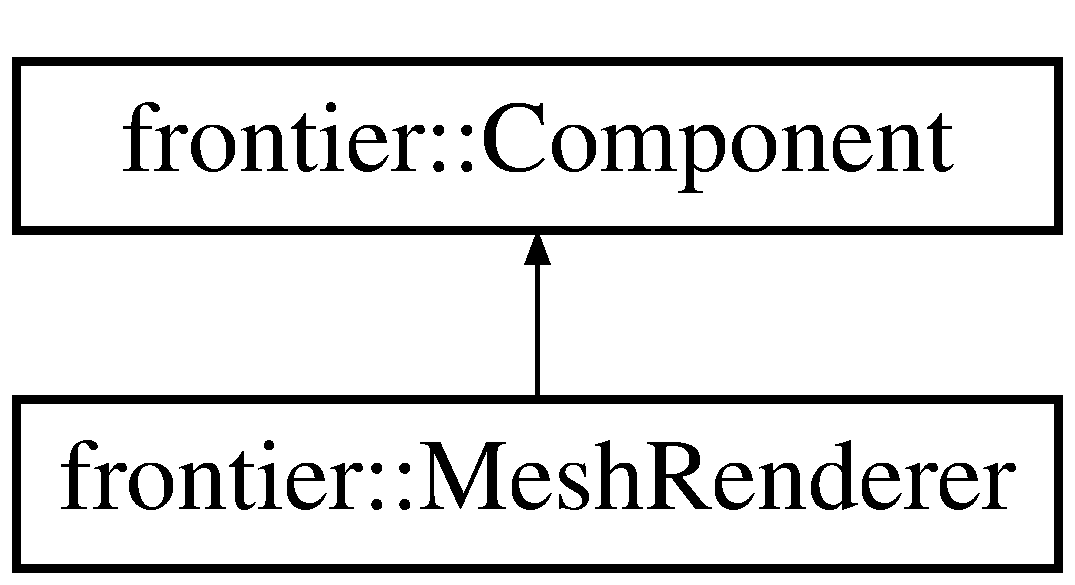
\includegraphics[height=2.000000cm]{classfrontier_1_1_mesh_renderer}
\end{center}
\end{figure}
\subsection*{Public Member Functions}
\begin{DoxyCompactItemize}
\item 
void \hyperlink{classfrontier_1_1_mesh_renderer_a3137cee27f2c38b49d31b7e944f8755c}{On\+Init} (std\+::weak\+\_\+ptr$<$ \hyperlink{classfrontier_1_1_entity}{Entity} $>$ \+\_\+parent, std\+::shared\+\_\+ptr$<$ \hyperlink{classfrontier_1_1_model}{Model} $>$ \+\_\+mesh\+Data)
\begin{DoxyCompactList}\small\item\em Initialises the \hyperlink{classfrontier_1_1_mesh_renderer}{Mesh\+Renderer} with a model. \end{DoxyCompactList}\item 
void \hyperlink{classfrontier_1_1_mesh_renderer_a27e5a0fdf24ffdae6555f2d132adf3f4}{On\+Init} (std\+::weak\+\_\+ptr$<$ \hyperlink{classfrontier_1_1_entity}{Entity} $>$ \+\_\+parent, std\+::weak\+\_\+ptr$<$ \hyperlink{classfrontier_1_1_mesh_renderer}{Mesh\+Renderer} $>$ \+\_\+original)
\begin{DoxyCompactList}\small\item\em Initialises the \hyperlink{classfrontier_1_1_mesh_renderer}{Mesh\+Renderer} with a \hyperlink{classfrontier_1_1_mesh_renderer}{Mesh\+Renderer}, usually from a prefab. \end{DoxyCompactList}\item 
void \hyperlink{classfrontier_1_1_mesh_renderer_acffde7174ddb009751e360df5d346922}{On\+Tick} () override
\begin{DoxyCompactList}\small\item\em Draws the mesh. \end{DoxyCompactList}\item 
void \hyperlink{classfrontier_1_1_mesh_renderer_a8be0a3e04dc5c9e56e230c914e58c2dc}{Attach\+Shader\+Program} (std\+::shared\+\_\+ptr$<$ \hyperlink{classfrontier_1_1_shader}{Shader} $>$ \+\_\+new\+Shader\+Program)
\begin{DoxyCompactList}\small\item\em Attaches a shader program to the mesh renderer. \end{DoxyCompactList}\item 
void \hyperlink{classfrontier_1_1_mesh_renderer_a5c915d5fba6a56841afe98123e8cfa5d}{Attach\+Texture} (std\+::shared\+\_\+ptr$<$ \hyperlink{classfrontier_1_1_texture}{Texture} $>$ \+\_\+new\+Texture)
\begin{DoxyCompactList}\small\item\em Attaches a texture to the mesh renderer. \end{DoxyCompactList}\item 
std\+::shared\+\_\+ptr$<$ \hyperlink{classfrontier_1_1_model}{Model} $>$ \hyperlink{classfrontier_1_1_mesh_renderer_a082036277e00227a57a16a542e2b57e3}{Get\+Mesh\+Data} ()
\begin{DoxyCompactList}\small\item\em Returns the current model. \end{DoxyCompactList}\item 
std\+::shared\+\_\+ptr$<$ \hyperlink{classfrontier_1_1_texture}{Texture} $>$ \hyperlink{classfrontier_1_1_mesh_renderer_a408e31822fdceac2dd5c85527c47b100}{Get\+Texture} ()
\begin{DoxyCompactList}\small\item\em Returns the current texture. \end{DoxyCompactList}\item 
std\+::shared\+\_\+ptr$<$ \hyperlink{classfrontier_1_1_shader}{Shader} $>$ \hyperlink{classfrontier_1_1_mesh_renderer_a55c8a2d3b8f64767e5b1bcf2a28ec044}{Get\+Shader} ()
\begin{DoxyCompactList}\small\item\em Returns the current shader. \end{DoxyCompactList}\end{DoxyCompactItemize}
\subsection*{Additional Inherited Members}


\subsection{Detailed Description}
Container for a model. 

\subsection{Member Function Documentation}
\mbox{\Hypertarget{classfrontier_1_1_mesh_renderer_a8be0a3e04dc5c9e56e230c914e58c2dc}\label{classfrontier_1_1_mesh_renderer_a8be0a3e04dc5c9e56e230c914e58c2dc}} 
\index{frontier\+::\+Mesh\+Renderer@{frontier\+::\+Mesh\+Renderer}!Attach\+Shader\+Program@{Attach\+Shader\+Program}}
\index{Attach\+Shader\+Program@{Attach\+Shader\+Program}!frontier\+::\+Mesh\+Renderer@{frontier\+::\+Mesh\+Renderer}}
\subsubsection{\texorpdfstring{Attach\+Shader\+Program()}{AttachShaderProgram()}}
{\footnotesize\ttfamily void frontier\+::\+Mesh\+Renderer\+::\+Attach\+Shader\+Program (\begin{DoxyParamCaption}\item[{std\+::shared\+\_\+ptr$<$ \hyperlink{classfrontier_1_1_shader}{Shader} $>$}]{\+\_\+new\+Shader\+Program }\end{DoxyParamCaption})}



Attaches a shader program to the mesh renderer. 


\begin{DoxyParams}{Parameters}
{\em \+\_\+new\+Shader\+Program} & \hyperlink{classfrontier_1_1_shader}{Shader} program to attach. \\
\hline
\end{DoxyParams}
\mbox{\Hypertarget{classfrontier_1_1_mesh_renderer_a5c915d5fba6a56841afe98123e8cfa5d}\label{classfrontier_1_1_mesh_renderer_a5c915d5fba6a56841afe98123e8cfa5d}} 
\index{frontier\+::\+Mesh\+Renderer@{frontier\+::\+Mesh\+Renderer}!Attach\+Texture@{Attach\+Texture}}
\index{Attach\+Texture@{Attach\+Texture}!frontier\+::\+Mesh\+Renderer@{frontier\+::\+Mesh\+Renderer}}
\subsubsection{\texorpdfstring{Attach\+Texture()}{AttachTexture()}}
{\footnotesize\ttfamily void frontier\+::\+Mesh\+Renderer\+::\+Attach\+Texture (\begin{DoxyParamCaption}\item[{std\+::shared\+\_\+ptr$<$ \hyperlink{classfrontier_1_1_texture}{Texture} $>$}]{\+\_\+new\+Texture }\end{DoxyParamCaption})}



Attaches a texture to the mesh renderer. 


\begin{DoxyParams}{Parameters}
{\em \+\_\+new\+Texture} & \hyperlink{classfrontier_1_1_texture}{Texture} to attach. \\
\hline
\end{DoxyParams}
\mbox{\Hypertarget{classfrontier_1_1_mesh_renderer_a082036277e00227a57a16a542e2b57e3}\label{classfrontier_1_1_mesh_renderer_a082036277e00227a57a16a542e2b57e3}} 
\index{frontier\+::\+Mesh\+Renderer@{frontier\+::\+Mesh\+Renderer}!Get\+Mesh\+Data@{Get\+Mesh\+Data}}
\index{Get\+Mesh\+Data@{Get\+Mesh\+Data}!frontier\+::\+Mesh\+Renderer@{frontier\+::\+Mesh\+Renderer}}
\subsubsection{\texorpdfstring{Get\+Mesh\+Data()}{GetMeshData()}}
{\footnotesize\ttfamily std\+::shared\+\_\+ptr$<$ \hyperlink{classfrontier_1_1_model}{Model} $>$ frontier\+::\+Mesh\+Renderer\+::\+Get\+Mesh\+Data (\begin{DoxyParamCaption}{ }\end{DoxyParamCaption})}



Returns the current model. 

\mbox{\Hypertarget{classfrontier_1_1_mesh_renderer_a55c8a2d3b8f64767e5b1bcf2a28ec044}\label{classfrontier_1_1_mesh_renderer_a55c8a2d3b8f64767e5b1bcf2a28ec044}} 
\index{frontier\+::\+Mesh\+Renderer@{frontier\+::\+Mesh\+Renderer}!Get\+Shader@{Get\+Shader}}
\index{Get\+Shader@{Get\+Shader}!frontier\+::\+Mesh\+Renderer@{frontier\+::\+Mesh\+Renderer}}
\subsubsection{\texorpdfstring{Get\+Shader()}{GetShader()}}
{\footnotesize\ttfamily std\+::shared\+\_\+ptr$<$ \hyperlink{classfrontier_1_1_shader}{Shader} $>$ frontier\+::\+Mesh\+Renderer\+::\+Get\+Shader (\begin{DoxyParamCaption}{ }\end{DoxyParamCaption})}



Returns the current shader. 

\mbox{\Hypertarget{classfrontier_1_1_mesh_renderer_a408e31822fdceac2dd5c85527c47b100}\label{classfrontier_1_1_mesh_renderer_a408e31822fdceac2dd5c85527c47b100}} 
\index{frontier\+::\+Mesh\+Renderer@{frontier\+::\+Mesh\+Renderer}!Get\+Texture@{Get\+Texture}}
\index{Get\+Texture@{Get\+Texture}!frontier\+::\+Mesh\+Renderer@{frontier\+::\+Mesh\+Renderer}}
\subsubsection{\texorpdfstring{Get\+Texture()}{GetTexture()}}
{\footnotesize\ttfamily std\+::shared\+\_\+ptr$<$ \hyperlink{classfrontier_1_1_texture}{Texture} $>$ frontier\+::\+Mesh\+Renderer\+::\+Get\+Texture (\begin{DoxyParamCaption}{ }\end{DoxyParamCaption})}



Returns the current texture. 

\mbox{\Hypertarget{classfrontier_1_1_mesh_renderer_a3137cee27f2c38b49d31b7e944f8755c}\label{classfrontier_1_1_mesh_renderer_a3137cee27f2c38b49d31b7e944f8755c}} 
\index{frontier\+::\+Mesh\+Renderer@{frontier\+::\+Mesh\+Renderer}!On\+Init@{On\+Init}}
\index{On\+Init@{On\+Init}!frontier\+::\+Mesh\+Renderer@{frontier\+::\+Mesh\+Renderer}}
\subsubsection{\texorpdfstring{On\+Init()}{OnInit()}\hspace{0.1cm}{\footnotesize\ttfamily [1/2]}}
{\footnotesize\ttfamily void frontier\+::\+Mesh\+Renderer\+::\+On\+Init (\begin{DoxyParamCaption}\item[{std\+::weak\+\_\+ptr$<$ \hyperlink{classfrontier_1_1_entity}{Entity} $>$}]{\+\_\+parent,  }\item[{std\+::shared\+\_\+ptr$<$ \hyperlink{classfrontier_1_1_model}{Model} $>$}]{\+\_\+mesh\+Data }\end{DoxyParamCaption})}



Initialises the \hyperlink{classfrontier_1_1_mesh_renderer}{Mesh\+Renderer} with a model. 


\begin{DoxyParams}{Parameters}
{\em \+\_\+parent} & The entity this component will be attached to. \\
\hline
{\em \+\_\+mesh\+Data} & The model that will be rendered. \\
\hline
\end{DoxyParams}
\mbox{\Hypertarget{classfrontier_1_1_mesh_renderer_a27e5a0fdf24ffdae6555f2d132adf3f4}\label{classfrontier_1_1_mesh_renderer_a27e5a0fdf24ffdae6555f2d132adf3f4}} 
\index{frontier\+::\+Mesh\+Renderer@{frontier\+::\+Mesh\+Renderer}!On\+Init@{On\+Init}}
\index{On\+Init@{On\+Init}!frontier\+::\+Mesh\+Renderer@{frontier\+::\+Mesh\+Renderer}}
\subsubsection{\texorpdfstring{On\+Init()}{OnInit()}\hspace{0.1cm}{\footnotesize\ttfamily [2/2]}}
{\footnotesize\ttfamily void frontier\+::\+Mesh\+Renderer\+::\+On\+Init (\begin{DoxyParamCaption}\item[{std\+::weak\+\_\+ptr$<$ \hyperlink{classfrontier_1_1_entity}{Entity} $>$}]{\+\_\+parent,  }\item[{std\+::weak\+\_\+ptr$<$ \hyperlink{classfrontier_1_1_mesh_renderer}{Mesh\+Renderer} $>$}]{\+\_\+original }\end{DoxyParamCaption})}



Initialises the \hyperlink{classfrontier_1_1_mesh_renderer}{Mesh\+Renderer} with a \hyperlink{classfrontier_1_1_mesh_renderer}{Mesh\+Renderer}, usually from a prefab. 


\begin{DoxyParams}{Parameters}
{\em \+\_\+parent} & The entity this component will be attached to. \\
\hline
{\em \+\_\+original} & The orginal mesh renderer that will be copied. \\
\hline
\end{DoxyParams}
\mbox{\Hypertarget{classfrontier_1_1_mesh_renderer_acffde7174ddb009751e360df5d346922}\label{classfrontier_1_1_mesh_renderer_acffde7174ddb009751e360df5d346922}} 
\index{frontier\+::\+Mesh\+Renderer@{frontier\+::\+Mesh\+Renderer}!On\+Tick@{On\+Tick}}
\index{On\+Tick@{On\+Tick}!frontier\+::\+Mesh\+Renderer@{frontier\+::\+Mesh\+Renderer}}
\subsubsection{\texorpdfstring{On\+Tick()}{OnTick()}}
{\footnotesize\ttfamily void frontier\+::\+Mesh\+Renderer\+::\+On\+Tick (\begin{DoxyParamCaption}{ }\end{DoxyParamCaption})\hspace{0.3cm}{\ttfamily [override]}, {\ttfamily [virtual]}}



Draws the mesh. 



Reimplemented from \hyperlink{classfrontier_1_1_component_ab920f9bc07ce051ebb5559c5a66508d1}{frontier\+::\+Component}.



The documentation for this class was generated from the following files\+:\begin{DoxyCompactItemize}
\item 
src/myengine/\hyperlink{_mesh_renderer_8h}{Mesh\+Renderer.\+h}\item 
src/myengine/\hyperlink{_mesh_renderer_8cpp}{Mesh\+Renderer.\+cpp}\end{DoxyCompactItemize}

\hypertarget{classfrontier_1_1_model}{}\section{frontier\+:\+:Model Class Reference}
\label{classfrontier_1_1_model}\index{frontier\+::\+Model@{frontier\+::\+Model}}


A group of meshes that make up a model.  




{\ttfamily \#include $<$Model.\+h$>$}

Inheritance diagram for frontier\+:\+:Model\+:\begin{figure}[H]
\begin{center}
\leavevmode
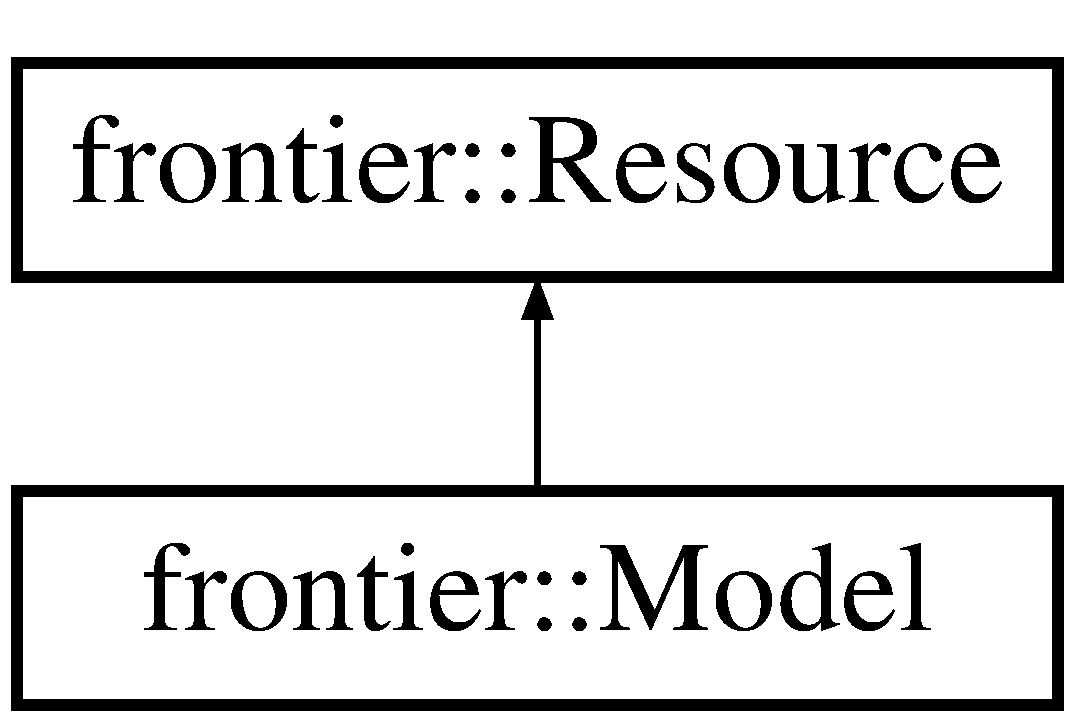
\includegraphics[height=2.000000cm]{classfrontier_1_1_model}
\end{center}
\end{figure}
\subsection*{Public Member Functions}
\begin{DoxyCompactItemize}
\item 
void \hyperlink{classfrontier_1_1_model_ab969b8ae4c222ac60f347a5008b19bad}{Draw} (glm\+::mat4 \+\_\+model, glm\+::mat4 \+\_\+view, glm\+::mat4 \+\_\+proj, std\+::shared\+\_\+ptr$<$ \hyperlink{classfrontier_1_1_texture}{Texture} $>$ \+\_\+tex, std\+::shared\+\_\+ptr$<$ \hyperlink{classfrontier_1_1_shader}{Shader} $>$ \+\_\+shader)
\begin{DoxyCompactList}\small\item\em Draws the model. \end{DoxyCompactList}\end{DoxyCompactItemize}
\subsection*{Static Public Member Functions}
\begin{DoxyCompactItemize}
\item 
static std\+::shared\+\_\+ptr$<$ \hyperlink{classfrontier_1_1_model}{Model} $>$ \hyperlink{classfrontier_1_1_model_a78f05cbc47e201551ccf3bbbd1d0fcbd}{Create} (const char $\ast$\+\_\+path, std\+::weak\+\_\+ptr$<$ \hyperlink{classfrontier_1_1_resources}{Resources} $>$ \+\_\+resources)
\begin{DoxyCompactList}\small\item\em Creates a model froma filepath to be used in a \hyperlink{classfrontier_1_1_mesh_renderer}{Mesh\+Renderer}. \end{DoxyCompactList}\end{DoxyCompactItemize}
\subsection*{Friends}
\begin{DoxyCompactItemize}
\item 
class \hyperlink{classfrontier_1_1_model_aa41a130f156b145bffb3f4b5172c4c93}{Mesh}
\end{DoxyCompactItemize}


\subsection{Detailed Description}
A group of meshes that make up a model. 

\subsection{Member Function Documentation}
\mbox{\Hypertarget{classfrontier_1_1_model_a78f05cbc47e201551ccf3bbbd1d0fcbd}\label{classfrontier_1_1_model_a78f05cbc47e201551ccf3bbbd1d0fcbd}} 
\index{frontier\+::\+Model@{frontier\+::\+Model}!Create@{Create}}
\index{Create@{Create}!frontier\+::\+Model@{frontier\+::\+Model}}
\subsubsection{\texorpdfstring{Create()}{Create()}}
{\footnotesize\ttfamily std\+::shared\+\_\+ptr$<$ \hyperlink{classfrontier_1_1_model}{Model} $>$ frontier\+::\+Model\+::\+Create (\begin{DoxyParamCaption}\item[{const char $\ast$}]{\+\_\+path,  }\item[{std\+::weak\+\_\+ptr$<$ \hyperlink{classfrontier_1_1_resources}{Resources} $>$}]{\+\_\+resources }\end{DoxyParamCaption})\hspace{0.3cm}{\ttfamily [static]}}



Creates a model froma filepath to be used in a \hyperlink{classfrontier_1_1_mesh_renderer}{Mesh\+Renderer}. 


\begin{DoxyParams}{Parameters}
{\em \+\_\+path} & The filepath for the model. \\
\hline
{\em \+\_\+resources} & The resources class located in core. \\
\hline
\end{DoxyParams}
\mbox{\Hypertarget{classfrontier_1_1_model_ab969b8ae4c222ac60f347a5008b19bad}\label{classfrontier_1_1_model_ab969b8ae4c222ac60f347a5008b19bad}} 
\index{frontier\+::\+Model@{frontier\+::\+Model}!Draw@{Draw}}
\index{Draw@{Draw}!frontier\+::\+Model@{frontier\+::\+Model}}
\subsubsection{\texorpdfstring{Draw()}{Draw()}}
{\footnotesize\ttfamily void frontier\+::\+Model\+::\+Draw (\begin{DoxyParamCaption}\item[{glm\+::mat4}]{\+\_\+model,  }\item[{glm\+::mat4}]{\+\_\+view,  }\item[{glm\+::mat4}]{\+\_\+proj,  }\item[{std\+::shared\+\_\+ptr$<$ \hyperlink{classfrontier_1_1_texture}{Texture} $>$}]{\+\_\+tex,  }\item[{std\+::shared\+\_\+ptr$<$ \hyperlink{classfrontier_1_1_shader}{Shader} $>$}]{\+\_\+shader }\end{DoxyParamCaption})}



Draws the model. 


\begin{DoxyParams}{Parameters}
{\em \+\_\+model} & The model matrix. \\
\hline
{\em \+\_\+view} & The view matrix, taken from the camera. \\
\hline
{\em \+\_\+proj} & The projection matrix, taken from the camera. \\
\hline
{\em \+\_\+tex} & The texture for the model. \\
\hline
{\em \+\_\+shader} & The shader for the model. \\
\hline
\end{DoxyParams}


\subsection{Friends And Related Function Documentation}
\mbox{\Hypertarget{classfrontier_1_1_model_aa41a130f156b145bffb3f4b5172c4c93}\label{classfrontier_1_1_model_aa41a130f156b145bffb3f4b5172c4c93}} 
\index{frontier\+::\+Model@{frontier\+::\+Model}!Mesh@{Mesh}}
\index{Mesh@{Mesh}!frontier\+::\+Model@{frontier\+::\+Model}}
\subsubsection{\texorpdfstring{Mesh}{Mesh}}
{\footnotesize\ttfamily friend class \hyperlink{classfrontier_1_1_mesh}{Mesh}\hspace{0.3cm}{\ttfamily [friend]}}



The documentation for this class was generated from the following files\+:\begin{DoxyCompactItemize}
\item 
src/myengine/\hyperlink{_model_8h}{Model.\+h}\item 
src/myengine/\hyperlink{_model_8cpp}{Model.\+cpp}\end{DoxyCompactItemize}

\hypertarget{class_player_controller}{}\section{Player\+Controller Class Reference}
\label{class_player_controller}\index{Player\+Controller@{Player\+Controller}}


{\ttfamily \#include $<$Player\+Controller.\+h$>$}

Inheritance diagram for Player\+Controller\+:\begin{figure}[H]
\begin{center}
\leavevmode
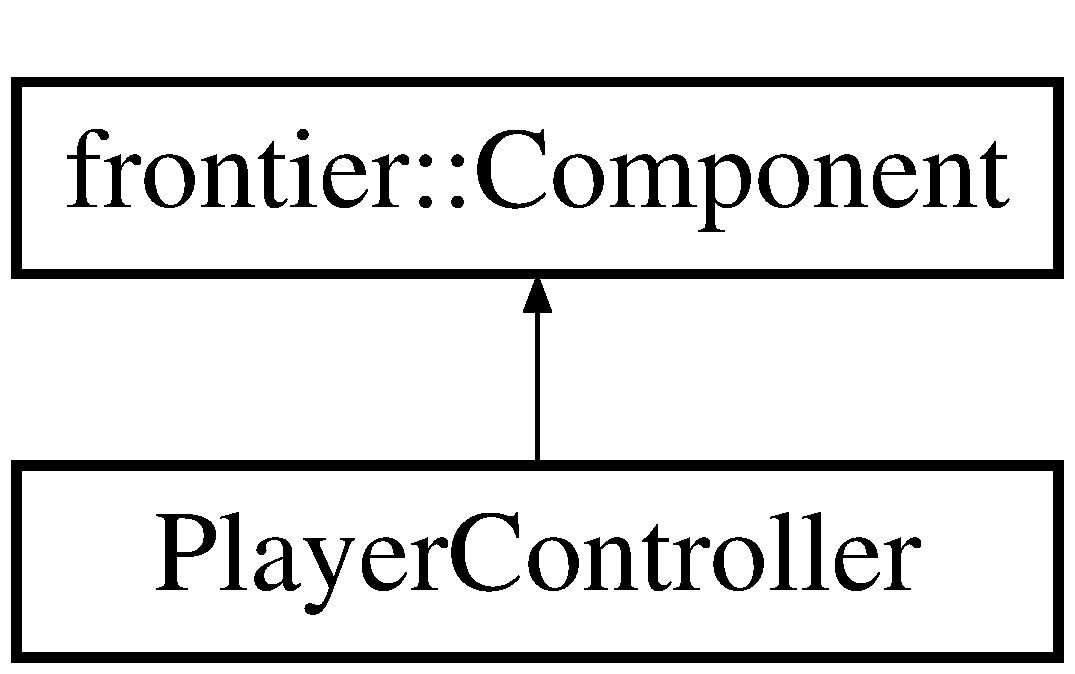
\includegraphics[height=2.000000cm]{class_player_controller}
\end{center}
\end{figure}
\subsection*{Public Member Functions}
\begin{DoxyCompactItemize}
\item 
void \hyperlink{class_player_controller_a22c60d9e4464ee585f3592593f14bc50}{On\+Init} (std\+::weak\+\_\+ptr$<$ \hyperlink{classfrontier_1_1_entity}{frontier\+::\+Entity} $>$ \+\_\+parent)
\item 
void \hyperlink{class_player_controller_a5641058df338563ff6bb6bce7645ef7b}{On\+Tick} () override
\item 
glm\+::vec3 \hyperlink{class_player_controller_a32543b8dc76ddb473c77afa03760e4d6}{get\+Forward\+Vector} ()
\item 
void \hyperlink{class_player_controller_a6fe2f80c8a3bac13c044e848b12f86ab}{set\+U\+I\+Icons} (std\+::weak\+\_\+ptr$<$ \hyperlink{classfrontier_1_1_entity}{frontier\+::\+Entity} $>$ \+\_\+icon1, std\+::weak\+\_\+ptr$<$ \hyperlink{classfrontier_1_1_entity}{frontier\+::\+Entity} $>$ \+\_\+icon2, std\+::weak\+\_\+ptr$<$ \hyperlink{classfrontier_1_1_entity}{frontier\+::\+Entity} $>$ \+\_\+icon3, std\+::weak\+\_\+ptr$<$ \hyperlink{classfrontier_1_1_entity}{frontier\+::\+Entity} $>$ \+\_\+game\+Over)
\item 
void \hyperlink{class_player_controller_a9bceb77b4a1d71290cc057ab16b64e8b}{set\+Audio\+Players} (std\+::weak\+\_\+ptr$<$ \hyperlink{classfrontier_1_1_audio_player}{frontier\+::\+Audio\+Player} $>$ \+\_\+shoot\+Sound, std\+::weak\+\_\+ptr$<$ \hyperlink{classfrontier_1_1_audio_player}{frontier\+::\+Audio\+Player} $>$ \+\_\+crash\+Sound)
\item 
void \hyperlink{class_player_controller_a7d329fd3ea21feff185a8d700e156a0c}{Hit} ()
\item 
bool \hyperlink{class_player_controller_a420a6722e37b0eb5219d4c2475c47041}{Is\+Game\+Over} ()
\item 
bool \hyperlink{class_player_controller_a8cd8a56ee0332aebb447db6a691aa639}{Is\+Invicible} ()
\end{DoxyCompactItemize}
\subsection*{Additional Inherited Members}


\subsection{Member Function Documentation}
\mbox{\Hypertarget{class_player_controller_a32543b8dc76ddb473c77afa03760e4d6}\label{class_player_controller_a32543b8dc76ddb473c77afa03760e4d6}} 
\index{Player\+Controller@{Player\+Controller}!get\+Forward\+Vector@{get\+Forward\+Vector}}
\index{get\+Forward\+Vector@{get\+Forward\+Vector}!Player\+Controller@{Player\+Controller}}
\subsubsection{\texorpdfstring{get\+Forward\+Vector()}{getForwardVector()}}
{\footnotesize\ttfamily glm\+::vec3 Player\+Controller\+::get\+Forward\+Vector (\begin{DoxyParamCaption}{ }\end{DoxyParamCaption})}

\mbox{\Hypertarget{class_player_controller_a7d329fd3ea21feff185a8d700e156a0c}\label{class_player_controller_a7d329fd3ea21feff185a8d700e156a0c}} 
\index{Player\+Controller@{Player\+Controller}!Hit@{Hit}}
\index{Hit@{Hit}!Player\+Controller@{Player\+Controller}}
\subsubsection{\texorpdfstring{Hit()}{Hit()}}
{\footnotesize\ttfamily void Player\+Controller\+::\+Hit (\begin{DoxyParamCaption}{ }\end{DoxyParamCaption})}

\mbox{\Hypertarget{class_player_controller_a420a6722e37b0eb5219d4c2475c47041}\label{class_player_controller_a420a6722e37b0eb5219d4c2475c47041}} 
\index{Player\+Controller@{Player\+Controller}!Is\+Game\+Over@{Is\+Game\+Over}}
\index{Is\+Game\+Over@{Is\+Game\+Over}!Player\+Controller@{Player\+Controller}}
\subsubsection{\texorpdfstring{Is\+Game\+Over()}{IsGameOver()}}
{\footnotesize\ttfamily bool Player\+Controller\+::\+Is\+Game\+Over (\begin{DoxyParamCaption}{ }\end{DoxyParamCaption})}

\mbox{\Hypertarget{class_player_controller_a8cd8a56ee0332aebb447db6a691aa639}\label{class_player_controller_a8cd8a56ee0332aebb447db6a691aa639}} 
\index{Player\+Controller@{Player\+Controller}!Is\+Invicible@{Is\+Invicible}}
\index{Is\+Invicible@{Is\+Invicible}!Player\+Controller@{Player\+Controller}}
\subsubsection{\texorpdfstring{Is\+Invicible()}{IsInvicible()}}
{\footnotesize\ttfamily bool Player\+Controller\+::\+Is\+Invicible (\begin{DoxyParamCaption}{ }\end{DoxyParamCaption})}

\mbox{\Hypertarget{class_player_controller_a22c60d9e4464ee585f3592593f14bc50}\label{class_player_controller_a22c60d9e4464ee585f3592593f14bc50}} 
\index{Player\+Controller@{Player\+Controller}!On\+Init@{On\+Init}}
\index{On\+Init@{On\+Init}!Player\+Controller@{Player\+Controller}}
\subsubsection{\texorpdfstring{On\+Init()}{OnInit()}}
{\footnotesize\ttfamily void Player\+Controller\+::\+On\+Init (\begin{DoxyParamCaption}\item[{std\+::weak\+\_\+ptr$<$ \hyperlink{classfrontier_1_1_entity}{frontier\+::\+Entity} $>$}]{\+\_\+parent }\end{DoxyParamCaption})\hspace{0.3cm}{\ttfamily [virtual]}}



Reimplemented from \hyperlink{classfrontier_1_1_component_af3da02905c4d79219d9b12f260a35ad1}{frontier\+::\+Component}.

\mbox{\Hypertarget{class_player_controller_a5641058df338563ff6bb6bce7645ef7b}\label{class_player_controller_a5641058df338563ff6bb6bce7645ef7b}} 
\index{Player\+Controller@{Player\+Controller}!On\+Tick@{On\+Tick}}
\index{On\+Tick@{On\+Tick}!Player\+Controller@{Player\+Controller}}
\subsubsection{\texorpdfstring{On\+Tick()}{OnTick()}}
{\footnotesize\ttfamily void Player\+Controller\+::\+On\+Tick (\begin{DoxyParamCaption}{ }\end{DoxyParamCaption})\hspace{0.3cm}{\ttfamily [override]}, {\ttfamily [virtual]}}



Reimplemented from \hyperlink{classfrontier_1_1_component_ab920f9bc07ce051ebb5559c5a66508d1}{frontier\+::\+Component}.

\mbox{\Hypertarget{class_player_controller_a9bceb77b4a1d71290cc057ab16b64e8b}\label{class_player_controller_a9bceb77b4a1d71290cc057ab16b64e8b}} 
\index{Player\+Controller@{Player\+Controller}!set\+Audio\+Players@{set\+Audio\+Players}}
\index{set\+Audio\+Players@{set\+Audio\+Players}!Player\+Controller@{Player\+Controller}}
\subsubsection{\texorpdfstring{set\+Audio\+Players()}{setAudioPlayers()}}
{\footnotesize\ttfamily void Player\+Controller\+::set\+Audio\+Players (\begin{DoxyParamCaption}\item[{std\+::weak\+\_\+ptr$<$ \hyperlink{classfrontier_1_1_audio_player}{frontier\+::\+Audio\+Player} $>$}]{\+\_\+shoot\+Sound,  }\item[{std\+::weak\+\_\+ptr$<$ \hyperlink{classfrontier_1_1_audio_player}{frontier\+::\+Audio\+Player} $>$}]{\+\_\+crash\+Sound }\end{DoxyParamCaption})}

\mbox{\Hypertarget{class_player_controller_a6fe2f80c8a3bac13c044e848b12f86ab}\label{class_player_controller_a6fe2f80c8a3bac13c044e848b12f86ab}} 
\index{Player\+Controller@{Player\+Controller}!set\+U\+I\+Icons@{set\+U\+I\+Icons}}
\index{set\+U\+I\+Icons@{set\+U\+I\+Icons}!Player\+Controller@{Player\+Controller}}
\subsubsection{\texorpdfstring{set\+U\+I\+Icons()}{setUIIcons()}}
{\footnotesize\ttfamily void Player\+Controller\+::set\+U\+I\+Icons (\begin{DoxyParamCaption}\item[{std\+::weak\+\_\+ptr$<$ \hyperlink{classfrontier_1_1_entity}{frontier\+::\+Entity} $>$}]{\+\_\+icon1,  }\item[{std\+::weak\+\_\+ptr$<$ \hyperlink{classfrontier_1_1_entity}{frontier\+::\+Entity} $>$}]{\+\_\+icon2,  }\item[{std\+::weak\+\_\+ptr$<$ \hyperlink{classfrontier_1_1_entity}{frontier\+::\+Entity} $>$}]{\+\_\+icon3,  }\item[{std\+::weak\+\_\+ptr$<$ \hyperlink{classfrontier_1_1_entity}{frontier\+::\+Entity} $>$}]{\+\_\+game\+Over }\end{DoxyParamCaption})}



The documentation for this class was generated from the following files\+:\begin{DoxyCompactItemize}
\item 
src/game/\hyperlink{_player_controller_8h}{Player\+Controller.\+h}\item 
src/game/\hyperlink{_player_controller_8cpp}{Player\+Controller.\+cpp}\end{DoxyCompactItemize}

\hypertarget{classfrontier_1_1_pooler}{}\section{frontier\+:\+:Pooler Class Reference}
\label{classfrontier_1_1_pooler}\index{frontier\+::\+Pooler@{frontier\+::\+Pooler}}


{\ttfamily \#include $<$Pooler.\+h$>$}

\subsection*{Public Member Functions}
\begin{DoxyCompactItemize}
\item 
void \hyperlink{classfrontier_1_1_pooler_ad62089e85f54e4cfa198f1f796e2bfea}{On\+Init} (std\+::weak\+\_\+ptr$<$ \hyperlink{classfrontier_1_1_core}{Core} $>$ \+\_\+core, std\+::string \+\_\+id, std\+::shared\+\_\+ptr$<$ \hyperlink{classfrontier_1_1_prefab}{Prefab} $>$ \+\_\+prefab, int initial\+Pool\+Size)
\item 
std\+::weak\+\_\+ptr$<$ \hyperlink{classfrontier_1_1_entity}{Entity} $>$ \hyperlink{classfrontier_1_1_pooler_acd7ce56f3b19b8fb6e4eb2ba94328573}{Spawn} (glm\+::vec3 \+\_\+position, bool modify\+Scale=false, glm\+::vec3 \+\_\+scale=glm\+::vec3(1.\+0f, 1.\+0f, 1.\+0f))
\item 
std\+::string \hyperlink{classfrontier_1_1_pooler_a5fb9072149f17191cdf585a4200561a9}{get\+ID} ()
\item 
int \hyperlink{classfrontier_1_1_pooler_a7b4e2884404c3c939b0d6feccade6a70}{get\+Active\+In\+Pool} ()
\item 
void \hyperlink{classfrontier_1_1_pooler_a67a23cf20cbe59488f26d0a9bd481e63}{deactivate\+All\+Instances} ()
\end{DoxyCompactItemize}


\subsection{Member Function Documentation}
\mbox{\Hypertarget{classfrontier_1_1_pooler_a67a23cf20cbe59488f26d0a9bd481e63}\label{classfrontier_1_1_pooler_a67a23cf20cbe59488f26d0a9bd481e63}} 
\index{frontier\+::\+Pooler@{frontier\+::\+Pooler}!deactivate\+All\+Instances@{deactivate\+All\+Instances}}
\index{deactivate\+All\+Instances@{deactivate\+All\+Instances}!frontier\+::\+Pooler@{frontier\+::\+Pooler}}
\subsubsection{\texorpdfstring{deactivate\+All\+Instances()}{deactivateAllInstances()}}
{\footnotesize\ttfamily void frontier\+::\+Pooler\+::deactivate\+All\+Instances (\begin{DoxyParamCaption}{ }\end{DoxyParamCaption})}

\mbox{\Hypertarget{classfrontier_1_1_pooler_a7b4e2884404c3c939b0d6feccade6a70}\label{classfrontier_1_1_pooler_a7b4e2884404c3c939b0d6feccade6a70}} 
\index{frontier\+::\+Pooler@{frontier\+::\+Pooler}!get\+Active\+In\+Pool@{get\+Active\+In\+Pool}}
\index{get\+Active\+In\+Pool@{get\+Active\+In\+Pool}!frontier\+::\+Pooler@{frontier\+::\+Pooler}}
\subsubsection{\texorpdfstring{get\+Active\+In\+Pool()}{getActiveInPool()}}
{\footnotesize\ttfamily int frontier\+::\+Pooler\+::get\+Active\+In\+Pool (\begin{DoxyParamCaption}{ }\end{DoxyParamCaption})}

\mbox{\Hypertarget{classfrontier_1_1_pooler_a5fb9072149f17191cdf585a4200561a9}\label{classfrontier_1_1_pooler_a5fb9072149f17191cdf585a4200561a9}} 
\index{frontier\+::\+Pooler@{frontier\+::\+Pooler}!get\+ID@{get\+ID}}
\index{get\+ID@{get\+ID}!frontier\+::\+Pooler@{frontier\+::\+Pooler}}
\subsubsection{\texorpdfstring{get\+I\+D()}{getID()}}
{\footnotesize\ttfamily std\+::string frontier\+::\+Pooler\+::get\+ID (\begin{DoxyParamCaption}{ }\end{DoxyParamCaption})}

\mbox{\Hypertarget{classfrontier_1_1_pooler_ad62089e85f54e4cfa198f1f796e2bfea}\label{classfrontier_1_1_pooler_ad62089e85f54e4cfa198f1f796e2bfea}} 
\index{frontier\+::\+Pooler@{frontier\+::\+Pooler}!On\+Init@{On\+Init}}
\index{On\+Init@{On\+Init}!frontier\+::\+Pooler@{frontier\+::\+Pooler}}
\subsubsection{\texorpdfstring{On\+Init()}{OnInit()}}
{\footnotesize\ttfamily void frontier\+::\+Pooler\+::\+On\+Init (\begin{DoxyParamCaption}\item[{std\+::weak\+\_\+ptr$<$ \hyperlink{classfrontier_1_1_core}{Core} $>$}]{\+\_\+core,  }\item[{std\+::string}]{\+\_\+id,  }\item[{std\+::shared\+\_\+ptr$<$ \hyperlink{classfrontier_1_1_prefab}{Prefab} $>$}]{\+\_\+prefab,  }\item[{int}]{initial\+Pool\+Size }\end{DoxyParamCaption})}

\mbox{\Hypertarget{classfrontier_1_1_pooler_acd7ce56f3b19b8fb6e4eb2ba94328573}\label{classfrontier_1_1_pooler_acd7ce56f3b19b8fb6e4eb2ba94328573}} 
\index{frontier\+::\+Pooler@{frontier\+::\+Pooler}!Spawn@{Spawn}}
\index{Spawn@{Spawn}!frontier\+::\+Pooler@{frontier\+::\+Pooler}}
\subsubsection{\texorpdfstring{Spawn()}{Spawn()}}
{\footnotesize\ttfamily std\+::weak\+\_\+ptr$<$ \hyperlink{classfrontier_1_1_entity}{Entity} $>$ frontier\+::\+Pooler\+::\+Spawn (\begin{DoxyParamCaption}\item[{glm\+::vec3}]{\+\_\+position,  }\item[{bool}]{modify\+Scale = {\ttfamily false},  }\item[{glm\+::vec3}]{\+\_\+scale = {\ttfamily glm\+:\+:vec3(1.0f,~1.0f,~1.0f)} }\end{DoxyParamCaption})}



The documentation for this class was generated from the following files\+:\begin{DoxyCompactItemize}
\item 
src/myengine/\hyperlink{_pooler_8h}{Pooler.\+h}\item 
src/myengine/\hyperlink{_pooler_8cpp}{Pooler.\+cpp}\end{DoxyCompactItemize}

\hypertarget{classfrontier_1_1_prefab}{}\section{frontier\+:\+:Prefab Class Reference}
\label{classfrontier_1_1_prefab}\index{frontier\+::\+Prefab@{frontier\+::\+Prefab}}


Acts as a template for an entity, can be passed into a new entity and the information stored will pass on to the new entity.  




{\ttfamily \#include $<$Prefab.\+h$>$}

Inheritance diagram for frontier\+:\+:Prefab\+:\begin{figure}[H]
\begin{center}
\leavevmode
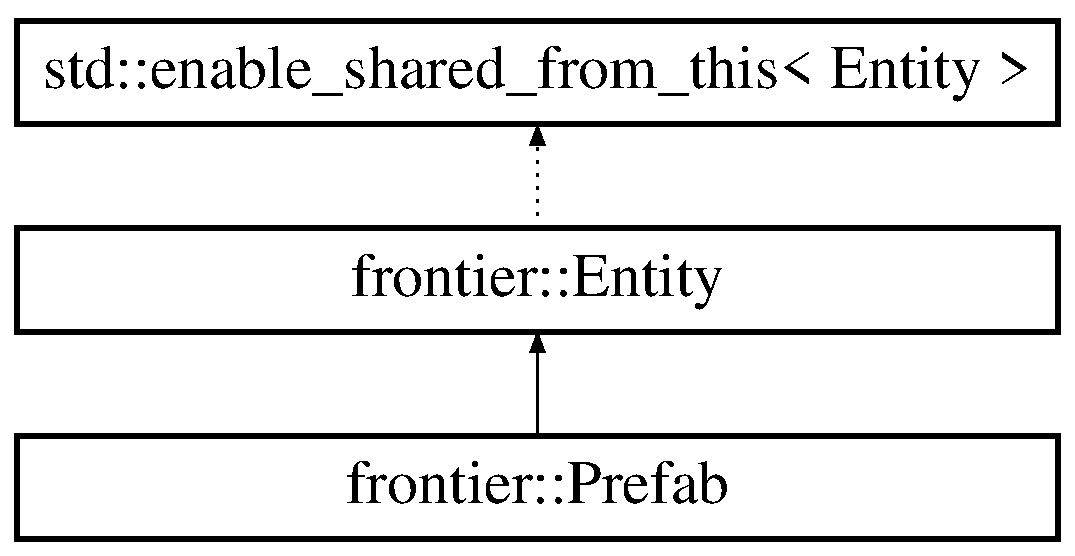
\includegraphics[height=3.000000cm]{classfrontier_1_1_prefab}
\end{center}
\end{figure}
\subsection*{Public Member Functions}
\begin{DoxyCompactItemize}
\item 
void \hyperlink{classfrontier_1_1_prefab_a69924d353fb96975efbba17dc0ba3f3a}{Init} (std\+::weak\+\_\+ptr$<$ \hyperlink{classfrontier_1_1_core}{Core} $>$ \+\_\+core\+Ptr) override
\begin{DoxyCompactList}\small\item\em Initialises the \hyperlink{classfrontier_1_1_prefab}{Prefab}. \end{DoxyCompactList}\item 
std\+::vector$<$ std\+::shared\+\_\+ptr$<$ \hyperlink{classfrontier_1_1_component}{Component} $>$ $>$ \hyperlink{classfrontier_1_1_prefab_a0d857efae6fb692384a6ab0144d66898}{get\+Components} ()
\begin{DoxyCompactList}\small\item\em Returns a vector of components attached to the prefab. \end{DoxyCompactList}\item 
{\footnotesize template$<$typename T $>$ }\\std\+::shared\+\_\+ptr$<$ T $>$ \hyperlink{classfrontier_1_1_prefab_a3099b0a889fb31500c7620bf96d878a1}{Add\+Component} ()
\begin{DoxyCompactList}\small\item\em Adds a component with no parameters in the initialiser. \end{DoxyCompactList}\item 
{\footnotesize template$<$typename T , typename A $>$ }\\std\+::shared\+\_\+ptr$<$ T $>$ \hyperlink{classfrontier_1_1_prefab_a96024d1688036fa4e6f7ec1a9d27b906}{Add\+Component} (A \+\_\+a)
\begin{DoxyCompactList}\small\item\em Adds a component with one parameters in the initialiser. \end{DoxyCompactList}\item 
{\footnotesize template$<$typename T , typename A , typename B $>$ }\\std\+::shared\+\_\+ptr$<$ T $>$ \hyperlink{classfrontier_1_1_prefab_acfe04a37ed21051b13f6c238505d654a}{Add\+Component} (A \+\_\+a, B \+\_\+b)
\begin{DoxyCompactList}\small\item\em Adds a component with two parameters in the initialiser. \end{DoxyCompactList}\item 
{\footnotesize template$<$typename T , typename A , typename B , typename C $>$ }\\std\+::shared\+\_\+ptr$<$ T $>$ \hyperlink{classfrontier_1_1_prefab_a6c7f7106b06aa35137eb9edc37221f68}{Add\+Component} (A \+\_\+a, B \+\_\+b, C \+\_\+c)
\begin{DoxyCompactList}\small\item\em Adds a component with three parameters in the initialiser. \end{DoxyCompactList}\item 
{\footnotesize template$<$typename T , typename A , typename B , typename C , typename D $>$ }\\std\+::shared\+\_\+ptr$<$ T $>$ \hyperlink{classfrontier_1_1_prefab_abee1253ab0b10d162df0b7729916a441}{Add\+Component} (A \+\_\+a, B \+\_\+b, C \+\_\+c, D \+\_\+d)
\begin{DoxyCompactList}\small\item\em Adds a component with four parameters in the initialiser. \end{DoxyCompactList}\item 
{\footnotesize template$<$typename T $>$ }\\std\+::shared\+\_\+ptr$<$ T $>$ \hyperlink{classfrontier_1_1_prefab_a54eab9e949addd7f9ed382893d60a56c}{Get\+Component} ()
\begin{DoxyCompactList}\small\item\em Returns a component of the specified type if one is attached. \end{DoxyCompactList}\end{DoxyCompactItemize}
\subsection*{Additional Inherited Members}


\subsection{Detailed Description}
Acts as a template for an entity, can be passed into a new entity and the information stored will pass on to the new entity. 

Currently, only these components will be copied into an entity\+: -\/collider -\/mesh renderer (with mesh, textures and shaders) -\/asteroid behaviour -\/projectile behaviour 

\subsection{Member Function Documentation}
\mbox{\Hypertarget{classfrontier_1_1_prefab_a3099b0a889fb31500c7620bf96d878a1}\label{classfrontier_1_1_prefab_a3099b0a889fb31500c7620bf96d878a1}} 
\index{frontier\+::\+Prefab@{frontier\+::\+Prefab}!Add\+Component@{Add\+Component}}
\index{Add\+Component@{Add\+Component}!frontier\+::\+Prefab@{frontier\+::\+Prefab}}
\subsubsection{\texorpdfstring{Add\+Component()}{AddComponent()}\hspace{0.1cm}{\footnotesize\ttfamily [1/5]}}
{\footnotesize\ttfamily template$<$typename T $>$ \\
std\+::shared\+\_\+ptr$<$T$>$ frontier\+::\+Prefab\+::\+Add\+Component (\begin{DoxyParamCaption}{ }\end{DoxyParamCaption})\hspace{0.3cm}{\ttfamily [inline]}}



Adds a component with no parameters in the initialiser. 

\mbox{\Hypertarget{classfrontier_1_1_prefab_a96024d1688036fa4e6f7ec1a9d27b906}\label{classfrontier_1_1_prefab_a96024d1688036fa4e6f7ec1a9d27b906}} 
\index{frontier\+::\+Prefab@{frontier\+::\+Prefab}!Add\+Component@{Add\+Component}}
\index{Add\+Component@{Add\+Component}!frontier\+::\+Prefab@{frontier\+::\+Prefab}}
\subsubsection{\texorpdfstring{Add\+Component()}{AddComponent()}\hspace{0.1cm}{\footnotesize\ttfamily [2/5]}}
{\footnotesize\ttfamily template$<$typename T , typename A $>$ \\
std\+::shared\+\_\+ptr$<$T$>$ frontier\+::\+Prefab\+::\+Add\+Component (\begin{DoxyParamCaption}\item[{A}]{\+\_\+a }\end{DoxyParamCaption})\hspace{0.3cm}{\ttfamily [inline]}}



Adds a component with one parameters in the initialiser. 

\mbox{\Hypertarget{classfrontier_1_1_prefab_acfe04a37ed21051b13f6c238505d654a}\label{classfrontier_1_1_prefab_acfe04a37ed21051b13f6c238505d654a}} 
\index{frontier\+::\+Prefab@{frontier\+::\+Prefab}!Add\+Component@{Add\+Component}}
\index{Add\+Component@{Add\+Component}!frontier\+::\+Prefab@{frontier\+::\+Prefab}}
\subsubsection{\texorpdfstring{Add\+Component()}{AddComponent()}\hspace{0.1cm}{\footnotesize\ttfamily [3/5]}}
{\footnotesize\ttfamily template$<$typename T , typename A , typename B $>$ \\
std\+::shared\+\_\+ptr$<$T$>$ frontier\+::\+Prefab\+::\+Add\+Component (\begin{DoxyParamCaption}\item[{A}]{\+\_\+a,  }\item[{B}]{\+\_\+b }\end{DoxyParamCaption})\hspace{0.3cm}{\ttfamily [inline]}}



Adds a component with two parameters in the initialiser. 

\mbox{\Hypertarget{classfrontier_1_1_prefab_a6c7f7106b06aa35137eb9edc37221f68}\label{classfrontier_1_1_prefab_a6c7f7106b06aa35137eb9edc37221f68}} 
\index{frontier\+::\+Prefab@{frontier\+::\+Prefab}!Add\+Component@{Add\+Component}}
\index{Add\+Component@{Add\+Component}!frontier\+::\+Prefab@{frontier\+::\+Prefab}}
\subsubsection{\texorpdfstring{Add\+Component()}{AddComponent()}\hspace{0.1cm}{\footnotesize\ttfamily [4/5]}}
{\footnotesize\ttfamily template$<$typename T , typename A , typename B , typename C $>$ \\
std\+::shared\+\_\+ptr$<$T$>$ frontier\+::\+Prefab\+::\+Add\+Component (\begin{DoxyParamCaption}\item[{A}]{\+\_\+a,  }\item[{B}]{\+\_\+b,  }\item[{C}]{\+\_\+c }\end{DoxyParamCaption})\hspace{0.3cm}{\ttfamily [inline]}}



Adds a component with three parameters in the initialiser. 

\mbox{\Hypertarget{classfrontier_1_1_prefab_abee1253ab0b10d162df0b7729916a441}\label{classfrontier_1_1_prefab_abee1253ab0b10d162df0b7729916a441}} 
\index{frontier\+::\+Prefab@{frontier\+::\+Prefab}!Add\+Component@{Add\+Component}}
\index{Add\+Component@{Add\+Component}!frontier\+::\+Prefab@{frontier\+::\+Prefab}}
\subsubsection{\texorpdfstring{Add\+Component()}{AddComponent()}\hspace{0.1cm}{\footnotesize\ttfamily [5/5]}}
{\footnotesize\ttfamily template$<$typename T , typename A , typename B , typename C , typename D $>$ \\
std\+::shared\+\_\+ptr$<$T$>$ frontier\+::\+Prefab\+::\+Add\+Component (\begin{DoxyParamCaption}\item[{A}]{\+\_\+a,  }\item[{B}]{\+\_\+b,  }\item[{C}]{\+\_\+c,  }\item[{D}]{\+\_\+d }\end{DoxyParamCaption})\hspace{0.3cm}{\ttfamily [inline]}}



Adds a component with four parameters in the initialiser. 

\mbox{\Hypertarget{classfrontier_1_1_prefab_a54eab9e949addd7f9ed382893d60a56c}\label{classfrontier_1_1_prefab_a54eab9e949addd7f9ed382893d60a56c}} 
\index{frontier\+::\+Prefab@{frontier\+::\+Prefab}!Get\+Component@{Get\+Component}}
\index{Get\+Component@{Get\+Component}!frontier\+::\+Prefab@{frontier\+::\+Prefab}}
\subsubsection{\texorpdfstring{Get\+Component()}{GetComponent()}}
{\footnotesize\ttfamily template$<$typename T $>$ \\
std\+::shared\+\_\+ptr$<$T$>$ frontier\+::\+Prefab\+::\+Get\+Component (\begin{DoxyParamCaption}{ }\end{DoxyParamCaption})\hspace{0.3cm}{\ttfamily [inline]}}



Returns a component of the specified type if one is attached. 

\mbox{\Hypertarget{classfrontier_1_1_prefab_a0d857efae6fb692384a6ab0144d66898}\label{classfrontier_1_1_prefab_a0d857efae6fb692384a6ab0144d66898}} 
\index{frontier\+::\+Prefab@{frontier\+::\+Prefab}!get\+Components@{get\+Components}}
\index{get\+Components@{get\+Components}!frontier\+::\+Prefab@{frontier\+::\+Prefab}}
\subsubsection{\texorpdfstring{get\+Components()}{getComponents()}}
{\footnotesize\ttfamily std\+::vector$<$ std\+::shared\+\_\+ptr$<$ \hyperlink{classfrontier_1_1_component}{Component} $>$ $>$ frontier\+::\+Prefab\+::get\+Components (\begin{DoxyParamCaption}{ }\end{DoxyParamCaption})}



Returns a vector of components attached to the prefab. 

\mbox{\Hypertarget{classfrontier_1_1_prefab_a69924d353fb96975efbba17dc0ba3f3a}\label{classfrontier_1_1_prefab_a69924d353fb96975efbba17dc0ba3f3a}} 
\index{frontier\+::\+Prefab@{frontier\+::\+Prefab}!Init@{Init}}
\index{Init@{Init}!frontier\+::\+Prefab@{frontier\+::\+Prefab}}
\subsubsection{\texorpdfstring{Init()}{Init()}}
{\footnotesize\ttfamily void frontier\+::\+Prefab\+::\+Init (\begin{DoxyParamCaption}\item[{std\+::weak\+\_\+ptr$<$ \hyperlink{classfrontier_1_1_core}{Core} $>$}]{\+\_\+core\+Ptr }\end{DoxyParamCaption})\hspace{0.3cm}{\ttfamily [override]}, {\ttfamily [virtual]}}



Initialises the \hyperlink{classfrontier_1_1_prefab}{Prefab}. 


\begin{DoxyParams}{Parameters}
{\em \+\_\+core\+Ptr} & Pointer to the core. \\
\hline
\end{DoxyParams}


Reimplemented from \hyperlink{classfrontier_1_1_entity_a94c998d26ccda48af3048eacd6d3c973}{frontier\+::\+Entity}.



The documentation for this class was generated from the following files\+:\begin{DoxyCompactItemize}
\item 
src/myengine/\hyperlink{_prefab_8h}{Prefab.\+h}\item 
src/myengine/\hyperlink{_prefab_8cpp}{Prefab.\+cpp}\end{DoxyCompactItemize}

\hypertarget{class_projectile_behavior}{}\section{Projectile\+Behavior Class Reference}
\label{class_projectile_behavior}\index{Projectile\+Behavior@{Projectile\+Behavior}}


{\ttfamily \#include $<$Projectile\+Behavior.\+h$>$}

Inheritance diagram for Projectile\+Behavior\+:\begin{figure}[H]
\begin{center}
\leavevmode
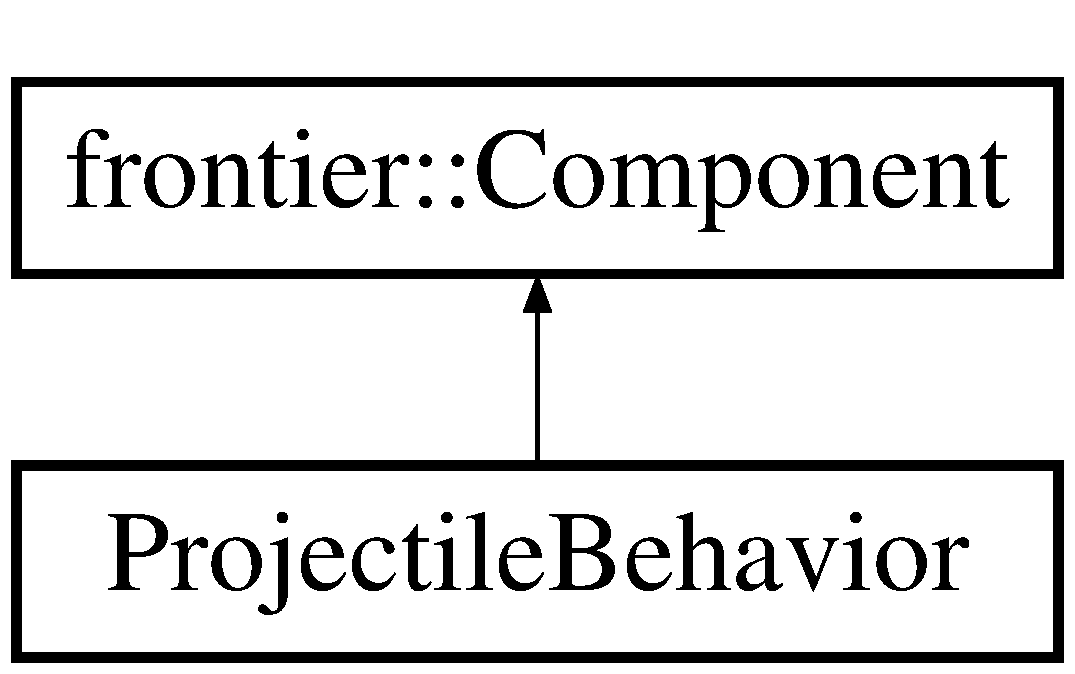
\includegraphics[height=2.000000cm]{class_projectile_behavior}
\end{center}
\end{figure}
\subsection*{Public Member Functions}
\begin{DoxyCompactItemize}
\item 
void \hyperlink{class_projectile_behavior_ab8caa701affecc1eaddb4bdc17152c23}{On\+Init} (std\+::weak\+\_\+ptr$<$ \hyperlink{classfrontier_1_1_entity}{frontier\+::\+Entity} $>$ \+\_\+parent, std\+::weak\+\_\+ptr$<$ \hyperlink{classfrontier_1_1_entity}{frontier\+::\+Entity} $>$ \+\_\+player)
\item 
void \hyperlink{class_projectile_behavior_a5e356eb4a161e7784c50b14ba39d98d1}{On\+Init} (std\+::weak\+\_\+ptr$<$ \hyperlink{classfrontier_1_1_entity}{frontier\+::\+Entity} $>$ \+\_\+parent, std\+::weak\+\_\+ptr$<$ \hyperlink{class_projectile_behavior}{Projectile\+Behavior} $>$ \+\_\+original)
\item 
void \hyperlink{class_projectile_behavior_a7756651ba998e7f3c0abcafcf25796ae}{On\+Tick} () override
\item 
void \hyperlink{class_projectile_behavior_aa01c813e541f6069d7ca9c69848ca0a6}{On\+Activate} () override
\item 
std\+::weak\+\_\+ptr$<$ \hyperlink{classfrontier_1_1_entity}{frontier\+::\+Entity} $>$ \hyperlink{class_projectile_behavior_ac0f47feec11bc48291c1d8721efe5bd8}{Get\+Player} ()
\end{DoxyCompactItemize}
\subsection*{Additional Inherited Members}


\subsection{Member Function Documentation}
\mbox{\Hypertarget{class_projectile_behavior_ac0f47feec11bc48291c1d8721efe5bd8}\label{class_projectile_behavior_ac0f47feec11bc48291c1d8721efe5bd8}} 
\index{Projectile\+Behavior@{Projectile\+Behavior}!Get\+Player@{Get\+Player}}
\index{Get\+Player@{Get\+Player}!Projectile\+Behavior@{Projectile\+Behavior}}
\subsubsection{\texorpdfstring{Get\+Player()}{GetPlayer()}}
{\footnotesize\ttfamily std\+::weak\+\_\+ptr$<$ \hyperlink{classfrontier_1_1_entity}{frontier\+::\+Entity} $>$ Projectile\+Behavior\+::\+Get\+Player (\begin{DoxyParamCaption}{ }\end{DoxyParamCaption})}

\mbox{\Hypertarget{class_projectile_behavior_aa01c813e541f6069d7ca9c69848ca0a6}\label{class_projectile_behavior_aa01c813e541f6069d7ca9c69848ca0a6}} 
\index{Projectile\+Behavior@{Projectile\+Behavior}!On\+Activate@{On\+Activate}}
\index{On\+Activate@{On\+Activate}!Projectile\+Behavior@{Projectile\+Behavior}}
\subsubsection{\texorpdfstring{On\+Activate()}{OnActivate()}}
{\footnotesize\ttfamily void Projectile\+Behavior\+::\+On\+Activate (\begin{DoxyParamCaption}{ }\end{DoxyParamCaption})\hspace{0.3cm}{\ttfamily [override]}, {\ttfamily [virtual]}}



Reimplemented from \hyperlink{classfrontier_1_1_component_a77fca7ba1960aafb9bc05905e300c79d}{frontier\+::\+Component}.

\mbox{\Hypertarget{class_projectile_behavior_ab8caa701affecc1eaddb4bdc17152c23}\label{class_projectile_behavior_ab8caa701affecc1eaddb4bdc17152c23}} 
\index{Projectile\+Behavior@{Projectile\+Behavior}!On\+Init@{On\+Init}}
\index{On\+Init@{On\+Init}!Projectile\+Behavior@{Projectile\+Behavior}}
\subsubsection{\texorpdfstring{On\+Init()}{OnInit()}\hspace{0.1cm}{\footnotesize\ttfamily [1/2]}}
{\footnotesize\ttfamily void Projectile\+Behavior\+::\+On\+Init (\begin{DoxyParamCaption}\item[{std\+::weak\+\_\+ptr$<$ \hyperlink{classfrontier_1_1_entity}{frontier\+::\+Entity} $>$}]{\+\_\+parent,  }\item[{std\+::weak\+\_\+ptr$<$ \hyperlink{classfrontier_1_1_entity}{frontier\+::\+Entity} $>$}]{\+\_\+player }\end{DoxyParamCaption})}

\mbox{\Hypertarget{class_projectile_behavior_a5e356eb4a161e7784c50b14ba39d98d1}\label{class_projectile_behavior_a5e356eb4a161e7784c50b14ba39d98d1}} 
\index{Projectile\+Behavior@{Projectile\+Behavior}!On\+Init@{On\+Init}}
\index{On\+Init@{On\+Init}!Projectile\+Behavior@{Projectile\+Behavior}}
\subsubsection{\texorpdfstring{On\+Init()}{OnInit()}\hspace{0.1cm}{\footnotesize\ttfamily [2/2]}}
{\footnotesize\ttfamily void Projectile\+Behavior\+::\+On\+Init (\begin{DoxyParamCaption}\item[{std\+::weak\+\_\+ptr$<$ \hyperlink{classfrontier_1_1_entity}{frontier\+::\+Entity} $>$}]{\+\_\+parent,  }\item[{std\+::weak\+\_\+ptr$<$ \hyperlink{class_projectile_behavior}{Projectile\+Behavior} $>$}]{\+\_\+original }\end{DoxyParamCaption})}

\mbox{\Hypertarget{class_projectile_behavior_a7756651ba998e7f3c0abcafcf25796ae}\label{class_projectile_behavior_a7756651ba998e7f3c0abcafcf25796ae}} 
\index{Projectile\+Behavior@{Projectile\+Behavior}!On\+Tick@{On\+Tick}}
\index{On\+Tick@{On\+Tick}!Projectile\+Behavior@{Projectile\+Behavior}}
\subsubsection{\texorpdfstring{On\+Tick()}{OnTick()}}
{\footnotesize\ttfamily void Projectile\+Behavior\+::\+On\+Tick (\begin{DoxyParamCaption}{ }\end{DoxyParamCaption})\hspace{0.3cm}{\ttfamily [override]}, {\ttfamily [virtual]}}



Reimplemented from \hyperlink{classfrontier_1_1_component_ab920f9bc07ce051ebb5559c5a66508d1}{frontier\+::\+Component}.



The documentation for this class was generated from the following files\+:\begin{DoxyCompactItemize}
\item 
src/game/\hyperlink{_projectile_behavior_8h}{Projectile\+Behavior.\+h}\item 
src/game/\hyperlink{_projectile_behavior_8cpp}{Projectile\+Behavior.\+cpp}\end{DoxyCompactItemize}

\hypertarget{classfrontier_1_1_resource}{}\section{frontier\+:\+:Resource Class Reference}
\label{classfrontier_1_1_resource}\index{frontier\+::\+Resource@{frontier\+::\+Resource}}


{\ttfamily \#include $<$Resource.\+h$>$}

Inheritance diagram for frontier\+:\+:Resource\+:\begin{figure}[H]
\begin{center}
\leavevmode
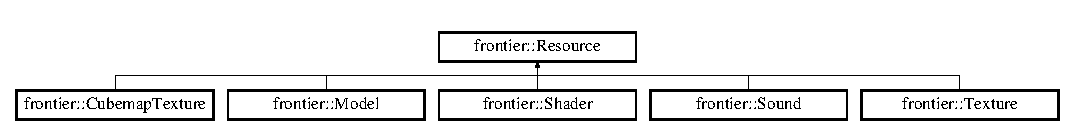
\includegraphics[height=1.382716cm]{classfrontier_1_1_resource}
\end{center}
\end{figure}
\subsection*{Public Member Functions}
\begin{DoxyCompactItemize}
\item 
\hyperlink{classfrontier_1_1_resource_a4ff9f98abc38d11f70b688a9886988c2}{Resource} ()
\item 
\hyperlink{classfrontier_1_1_resource_aea4c158b678419246b21b69ef27ffca6}{Resource} (std\+::string \+\_\+path\+Str)
\item 
\hyperlink{classfrontier_1_1_resource_a3bad96aa980d5300ddce81602a8d2f91}{$\sim$\+Resource} ()
\end{DoxyCompactItemize}
\subsection*{Protected Attributes}
\begin{DoxyCompactItemize}
\item 
std\+::string \hyperlink{classfrontier_1_1_resource_a69fe22a83fc57a08efd043e2c37edf7a}{\+\_\+path}
\end{DoxyCompactItemize}


\subsection{Constructor \& Destructor Documentation}
\mbox{\Hypertarget{classfrontier_1_1_resource_a4ff9f98abc38d11f70b688a9886988c2}\label{classfrontier_1_1_resource_a4ff9f98abc38d11f70b688a9886988c2}} 
\index{frontier\+::\+Resource@{frontier\+::\+Resource}!Resource@{Resource}}
\index{Resource@{Resource}!frontier\+::\+Resource@{frontier\+::\+Resource}}
\subsubsection{\texorpdfstring{Resource()}{Resource()}\hspace{0.1cm}{\footnotesize\ttfamily [1/2]}}
{\footnotesize\ttfamily frontier\+::\+Resource\+::\+Resource (\begin{DoxyParamCaption}{ }\end{DoxyParamCaption})}

\mbox{\Hypertarget{classfrontier_1_1_resource_aea4c158b678419246b21b69ef27ffca6}\label{classfrontier_1_1_resource_aea4c158b678419246b21b69ef27ffca6}} 
\index{frontier\+::\+Resource@{frontier\+::\+Resource}!Resource@{Resource}}
\index{Resource@{Resource}!frontier\+::\+Resource@{frontier\+::\+Resource}}
\subsubsection{\texorpdfstring{Resource()}{Resource()}\hspace{0.1cm}{\footnotesize\ttfamily [2/2]}}
{\footnotesize\ttfamily frontier\+::\+Resource\+::\+Resource (\begin{DoxyParamCaption}\item[{std\+::string}]{\+\_\+path\+Str }\end{DoxyParamCaption})}

\mbox{\Hypertarget{classfrontier_1_1_resource_a3bad96aa980d5300ddce81602a8d2f91}\label{classfrontier_1_1_resource_a3bad96aa980d5300ddce81602a8d2f91}} 
\index{frontier\+::\+Resource@{frontier\+::\+Resource}!````~Resource@{$\sim$\+Resource}}
\index{````~Resource@{$\sim$\+Resource}!frontier\+::\+Resource@{frontier\+::\+Resource}}
\subsubsection{\texorpdfstring{$\sim$\+Resource()}{~Resource()}}
{\footnotesize\ttfamily frontier\+::\+Resource\+::$\sim$\+Resource (\begin{DoxyParamCaption}{ }\end{DoxyParamCaption})}



\subsection{Member Data Documentation}
\mbox{\Hypertarget{classfrontier_1_1_resource_a69fe22a83fc57a08efd043e2c37edf7a}\label{classfrontier_1_1_resource_a69fe22a83fc57a08efd043e2c37edf7a}} 
\index{frontier\+::\+Resource@{frontier\+::\+Resource}!\+\_\+path@{\+\_\+path}}
\index{\+\_\+path@{\+\_\+path}!frontier\+::\+Resource@{frontier\+::\+Resource}}
\subsubsection{\texorpdfstring{\+\_\+path}{\_path}}
{\footnotesize\ttfamily std\+::string frontier\+::\+Resource\+::\+\_\+path\hspace{0.3cm}{\ttfamily [protected]}}



The documentation for this class was generated from the following files\+:\begin{DoxyCompactItemize}
\item 
src/myengine/\hyperlink{_resource_8h}{Resource.\+h}\item 
src/myengine/\hyperlink{_resource_8cpp}{Resource.\+cpp}\end{DoxyCompactItemize}

\hypertarget{classfrontier_1_1_resources}{}\section{frontier\+:\+:Resources Class Reference}
\label{classfrontier_1_1_resources}\index{frontier\+::\+Resources@{frontier\+::\+Resources}}


{\ttfamily \#include $<$Resources.\+h$>$}

\subsection*{Public Member Functions}
\begin{DoxyCompactItemize}
\item 
\hyperlink{classfrontier_1_1_resources_abd97410717435c463dccdb6e2d45043c}{Resources} ()
\item 
\hyperlink{classfrontier_1_1_resources_aa286a888a19e4ea5b5a94aa7ac1898b8}{$\sim$\+Resources} ()
\item 
void \hyperlink{classfrontier_1_1_resources_a34e0df1d6b935644bccee94ebe600a4a}{Add\+Created\+Resource} (std\+::shared\+\_\+ptr$<$ \hyperlink{classfrontier_1_1_resource}{Resource} $>$ \+\_\+resource)
\end{DoxyCompactItemize}


\subsection{Constructor \& Destructor Documentation}
\mbox{\Hypertarget{classfrontier_1_1_resources_abd97410717435c463dccdb6e2d45043c}\label{classfrontier_1_1_resources_abd97410717435c463dccdb6e2d45043c}} 
\index{frontier\+::\+Resources@{frontier\+::\+Resources}!Resources@{Resources}}
\index{Resources@{Resources}!frontier\+::\+Resources@{frontier\+::\+Resources}}
\subsubsection{\texorpdfstring{Resources()}{Resources()}}
{\footnotesize\ttfamily frontier\+::\+Resources\+::\+Resources (\begin{DoxyParamCaption}{ }\end{DoxyParamCaption})}

\mbox{\Hypertarget{classfrontier_1_1_resources_aa286a888a19e4ea5b5a94aa7ac1898b8}\label{classfrontier_1_1_resources_aa286a888a19e4ea5b5a94aa7ac1898b8}} 
\index{frontier\+::\+Resources@{frontier\+::\+Resources}!````~Resources@{$\sim$\+Resources}}
\index{````~Resources@{$\sim$\+Resources}!frontier\+::\+Resources@{frontier\+::\+Resources}}
\subsubsection{\texorpdfstring{$\sim$\+Resources()}{~Resources()}}
{\footnotesize\ttfamily frontier\+::\+Resources\+::$\sim$\+Resources (\begin{DoxyParamCaption}{ }\end{DoxyParamCaption})}



\subsection{Member Function Documentation}
\mbox{\Hypertarget{classfrontier_1_1_resources_a34e0df1d6b935644bccee94ebe600a4a}\label{classfrontier_1_1_resources_a34e0df1d6b935644bccee94ebe600a4a}} 
\index{frontier\+::\+Resources@{frontier\+::\+Resources}!Add\+Created\+Resource@{Add\+Created\+Resource}}
\index{Add\+Created\+Resource@{Add\+Created\+Resource}!frontier\+::\+Resources@{frontier\+::\+Resources}}
\subsubsection{\texorpdfstring{Add\+Created\+Resource()}{AddCreatedResource()}}
{\footnotesize\ttfamily void frontier\+::\+Resources\+::\+Add\+Created\+Resource (\begin{DoxyParamCaption}\item[{std\+::shared\+\_\+ptr$<$ \hyperlink{classfrontier_1_1_resource}{Resource} $>$}]{\+\_\+resource }\end{DoxyParamCaption})}



The documentation for this class was generated from the following files\+:\begin{DoxyCompactItemize}
\item 
src/myengine/\hyperlink{_resources_8h}{Resources.\+h}\item 
src/myengine/\hyperlink{_resources_8cpp}{Resources.\+cpp}\end{DoxyCompactItemize}

\hypertarget{classfrontier_1_1_shader}{}\section{frontier\+:\+:Shader Class Reference}
\label{classfrontier_1_1_shader}\index{frontier\+::\+Shader@{frontier\+::\+Shader}}


A container for a shader. Compiles a shader from filepaths.  




{\ttfamily \#include $<$Shader.\+h$>$}

Inheritance diagram for frontier\+:\+:Shader\+:\begin{figure}[H]
\begin{center}
\leavevmode
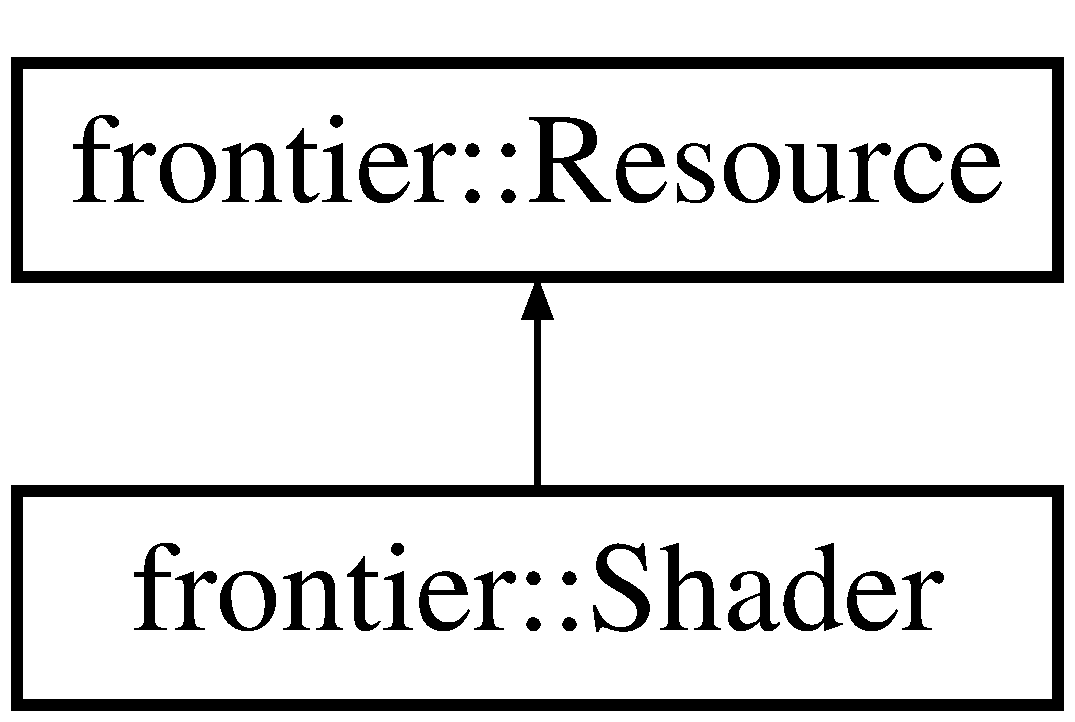
\includegraphics[height=2.000000cm]{classfrontier_1_1_shader}
\end{center}
\end{figure}
\subsection*{Public Member Functions}
\begin{DoxyCompactItemize}
\item 
void \hyperlink{classfrontier_1_1_shader_ae893f9f790c70ef2abaa0f1ba58bfec1}{Set\+Uniform} (const G\+Lchar $\ast$\+\_\+name, float \+\_\+value, bool \+\_\+unset\+Program=false)
\begin{DoxyCompactList}\small\item\em Sets a float uniform. \end{DoxyCompactList}\item 
void \hyperlink{classfrontier_1_1_shader_ae11b17bf3cc75186024f9a058cf06cb7}{Set\+Uniform} (const G\+Lchar $\ast$\+\_\+name, int \+\_\+value, bool \+\_\+unset\+Program=false)
\begin{DoxyCompactList}\small\item\em Sets an int uniform. \end{DoxyCompactList}\item 
void \hyperlink{classfrontier_1_1_shader_ad9bb90b3f092c6925293cee5013c9400}{Set\+Uniform} (const G\+Lchar $\ast$\+\_\+name, std\+::weak\+\_\+ptr$<$ \hyperlink{classfrontier_1_1_texture}{Texture} $>$ \+\_\+texture, bool \+\_\+unset\+Program=false)
\begin{DoxyCompactList}\small\item\em Sets a texture uniform. \end{DoxyCompactList}\item 
void \hyperlink{classfrontier_1_1_shader_a801d8cdbe9d924c601fddcdf9744c0d3}{Set\+Uniform} (const G\+Lchar $\ast$\+\_\+name, std\+::weak\+\_\+ptr$<$ \hyperlink{classfrontier_1_1_cubemap_texture}{Cubemap\+Texture} $>$ \+\_\+texture, bool \+\_\+unsetprogram=false)
\begin{DoxyCompactList}\small\item\em Sets a cubemap uniform. \end{DoxyCompactList}\item 
void \hyperlink{classfrontier_1_1_shader_adebc3dfdc6b24535ed01cfc5a8f69867}{Set\+Uniform} (const G\+Lchar $\ast$\+\_\+name, glm\+::mat4 \+\_\+value, bool \+\_\+unset\+Program=false, bool \+\_\+transpose=false)
\begin{DoxyCompactList}\small\item\em Sets a mat4 uniform. \end{DoxyCompactList}\item 
void \hyperlink{classfrontier_1_1_shader_aad5527a4747c3dc7692a8cdaede42537}{Set\+Uniform} (const G\+Lchar $\ast$\+\_\+name, glm\+::vec3 \+\_\+value, bool \+\_\+unset\+Program=false)
\begin{DoxyCompactList}\small\item\em Sets a vec3 uniform. \end{DoxyCompactList}\item 
void \hyperlink{classfrontier_1_1_shader_a2f1cc89390360779c0df68f2d10efff1}{Set\+Uniform} (const G\+Lchar $\ast$\+\_\+name, glm\+::vec4 \+\_\+value, bool \+\_\+unset\+Program=false)
\begin{DoxyCompactList}\small\item\em Sets a vec4 uniform. \end{DoxyCompactList}\item 
void \hyperlink{classfrontier_1_1_shader_a2485d4542cb287c9831558ed1cbd0d13}{Set\+ID} (G\+Luint \+\_\+new\+ID)
\begin{DoxyCompactList}\small\item\em Sets a new ID for the \hyperlink{classfrontier_1_1_shader}{Shader}. \end{DoxyCompactList}\item 
G\+Luint \hyperlink{classfrontier_1_1_shader_a3536975966e61e614e544d1bba702383}{Get\+ID} ()
\begin{DoxyCompactList}\small\item\em Returns the current ID for the \hyperlink{classfrontier_1_1_shader}{Shader}. \end{DoxyCompactList}\end{DoxyCompactItemize}
\subsection*{Static Public Member Functions}
\begin{DoxyCompactItemize}
\item 
static std\+::shared\+\_\+ptr$<$ \hyperlink{classfrontier_1_1_shader}{Shader} $>$ \hyperlink{classfrontier_1_1_shader_add4c33f617fa62cc1d0757a875bacd01}{Create} (std\+::string \+\_\+frag\+Scr, std\+::string \+\_\+vert\+Scr, std\+::vector$<$ G\+Lchar $\ast$$>$ \+\_\+attributes, std\+::shared\+\_\+ptr$<$ \hyperlink{classfrontier_1_1_resources}{Resources} $>$ \+\_\+resources)
\begin{DoxyCompactList}\small\item\em Creates and compiles a new shader and returns a pointer. \end{DoxyCompactList}\end{DoxyCompactItemize}


\subsection{Detailed Description}
A container for a shader. Compiles a shader from filepaths. 

\subsection{Member Function Documentation}
\mbox{\Hypertarget{classfrontier_1_1_shader_add4c33f617fa62cc1d0757a875bacd01}\label{classfrontier_1_1_shader_add4c33f617fa62cc1d0757a875bacd01}} 
\index{frontier\+::\+Shader@{frontier\+::\+Shader}!Create@{Create}}
\index{Create@{Create}!frontier\+::\+Shader@{frontier\+::\+Shader}}
\subsubsection{\texorpdfstring{Create()}{Create()}}
{\footnotesize\ttfamily std\+::shared\+\_\+ptr$<$ \hyperlink{classfrontier_1_1_shader}{Shader} $>$ frontier\+::\+Shader\+::\+Create (\begin{DoxyParamCaption}\item[{std\+::string}]{\+\_\+frag\+Scr,  }\item[{std\+::string}]{\+\_\+vert\+Scr,  }\item[{std\+::vector$<$ G\+Lchar $\ast$$>$}]{\+\_\+attributes,  }\item[{std\+::shared\+\_\+ptr$<$ \hyperlink{classfrontier_1_1_resources}{Resources} $>$}]{\+\_\+resources }\end{DoxyParamCaption})\hspace{0.3cm}{\ttfamily [static]}}



Creates and compiles a new shader and returns a pointer. 


\begin{DoxyParams}{Parameters}
{\em \+\_\+frag\+Src} & The filepath of the fragment shader. \\
\hline
{\em \+\_\+vert\+Src} & The filepath of the vertex shader. \\
\hline
{\em \+\_\+attributes} & A list of the attributes used in the shader. \\
\hline
{\em \+\_\+resources} & A pointer to the resources class so that the shader can be refered back to later. \\
\hline
\end{DoxyParams}
\mbox{\Hypertarget{classfrontier_1_1_shader_a3536975966e61e614e544d1bba702383}\label{classfrontier_1_1_shader_a3536975966e61e614e544d1bba702383}} 
\index{frontier\+::\+Shader@{frontier\+::\+Shader}!Get\+ID@{Get\+ID}}
\index{Get\+ID@{Get\+ID}!frontier\+::\+Shader@{frontier\+::\+Shader}}
\subsubsection{\texorpdfstring{Get\+I\+D()}{GetID()}}
{\footnotesize\ttfamily G\+Luint frontier\+::\+Shader\+::\+Get\+ID (\begin{DoxyParamCaption}{ }\end{DoxyParamCaption})}



Returns the current ID for the \hyperlink{classfrontier_1_1_shader}{Shader}. 

\mbox{\Hypertarget{classfrontier_1_1_shader_a2485d4542cb287c9831558ed1cbd0d13}\label{classfrontier_1_1_shader_a2485d4542cb287c9831558ed1cbd0d13}} 
\index{frontier\+::\+Shader@{frontier\+::\+Shader}!Set\+ID@{Set\+ID}}
\index{Set\+ID@{Set\+ID}!frontier\+::\+Shader@{frontier\+::\+Shader}}
\subsubsection{\texorpdfstring{Set\+I\+D()}{SetID()}}
{\footnotesize\ttfamily void frontier\+::\+Shader\+::\+Set\+ID (\begin{DoxyParamCaption}\item[{G\+Luint}]{\+\_\+new\+ID }\end{DoxyParamCaption})}



Sets a new ID for the \hyperlink{classfrontier_1_1_shader}{Shader}. 


\begin{DoxyParams}{Parameters}
{\em \+\_\+new\+ID} & The new ID for the shader. \\
\hline
\end{DoxyParams}
\mbox{\Hypertarget{classfrontier_1_1_shader_ae893f9f790c70ef2abaa0f1ba58bfec1}\label{classfrontier_1_1_shader_ae893f9f790c70ef2abaa0f1ba58bfec1}} 
\index{frontier\+::\+Shader@{frontier\+::\+Shader}!Set\+Uniform@{Set\+Uniform}}
\index{Set\+Uniform@{Set\+Uniform}!frontier\+::\+Shader@{frontier\+::\+Shader}}
\subsubsection{\texorpdfstring{Set\+Uniform()}{SetUniform()}\hspace{0.1cm}{\footnotesize\ttfamily [1/7]}}
{\footnotesize\ttfamily void frontier\+::\+Shader\+::\+Set\+Uniform (\begin{DoxyParamCaption}\item[{const G\+Lchar $\ast$}]{\+\_\+name,  }\item[{float}]{\+\_\+value,  }\item[{bool}]{\+\_\+unset\+Program = {\ttfamily false} }\end{DoxyParamCaption})}



Sets a float uniform. 


\begin{DoxyParams}{Parameters}
{\em \+\_\+name} & The name of the uniform \\
\hline
{\em \+\_\+value} & The value of the uniform \\
\hline
{\em \+\_\+unset\+Program} & Whether to set open\+GL back to a null shader after the uniform has been set. \\
\hline
\end{DoxyParams}
\mbox{\Hypertarget{classfrontier_1_1_shader_ae11b17bf3cc75186024f9a058cf06cb7}\label{classfrontier_1_1_shader_ae11b17bf3cc75186024f9a058cf06cb7}} 
\index{frontier\+::\+Shader@{frontier\+::\+Shader}!Set\+Uniform@{Set\+Uniform}}
\index{Set\+Uniform@{Set\+Uniform}!frontier\+::\+Shader@{frontier\+::\+Shader}}
\subsubsection{\texorpdfstring{Set\+Uniform()}{SetUniform()}\hspace{0.1cm}{\footnotesize\ttfamily [2/7]}}
{\footnotesize\ttfamily void frontier\+::\+Shader\+::\+Set\+Uniform (\begin{DoxyParamCaption}\item[{const G\+Lchar $\ast$}]{\+\_\+name,  }\item[{int}]{\+\_\+value,  }\item[{bool}]{\+\_\+unset\+Program = {\ttfamily false} }\end{DoxyParamCaption})}



Sets an int uniform. 


\begin{DoxyParams}{Parameters}
{\em \+\_\+name} & The name of the uniform \\
\hline
{\em \+\_\+value} & The value of the uniform \\
\hline
{\em \+\_\+unset\+Program} & Whether to set open\+GL back to a null shader after the uniform has been set. \\
\hline
\end{DoxyParams}
\mbox{\Hypertarget{classfrontier_1_1_shader_ad9bb90b3f092c6925293cee5013c9400}\label{classfrontier_1_1_shader_ad9bb90b3f092c6925293cee5013c9400}} 
\index{frontier\+::\+Shader@{frontier\+::\+Shader}!Set\+Uniform@{Set\+Uniform}}
\index{Set\+Uniform@{Set\+Uniform}!frontier\+::\+Shader@{frontier\+::\+Shader}}
\subsubsection{\texorpdfstring{Set\+Uniform()}{SetUniform()}\hspace{0.1cm}{\footnotesize\ttfamily [3/7]}}
{\footnotesize\ttfamily void frontier\+::\+Shader\+::\+Set\+Uniform (\begin{DoxyParamCaption}\item[{const G\+Lchar $\ast$}]{\+\_\+name,  }\item[{std\+::weak\+\_\+ptr$<$ \hyperlink{classfrontier_1_1_texture}{Texture} $>$}]{\+\_\+texture,  }\item[{bool}]{\+\_\+unset\+Program = {\ttfamily false} }\end{DoxyParamCaption})}



Sets a texture uniform. 


\begin{DoxyParams}{Parameters}
{\em \+\_\+name} & The name of the uniform \\
\hline
{\em \+\_\+texture} & The value of the uniform \\
\hline
{\em \+\_\+unset\+Program} & Whether to set open\+GL back to a null shader after the uniform has been set. \\
\hline
\end{DoxyParams}
\mbox{\Hypertarget{classfrontier_1_1_shader_a801d8cdbe9d924c601fddcdf9744c0d3}\label{classfrontier_1_1_shader_a801d8cdbe9d924c601fddcdf9744c0d3}} 
\index{frontier\+::\+Shader@{frontier\+::\+Shader}!Set\+Uniform@{Set\+Uniform}}
\index{Set\+Uniform@{Set\+Uniform}!frontier\+::\+Shader@{frontier\+::\+Shader}}
\subsubsection{\texorpdfstring{Set\+Uniform()}{SetUniform()}\hspace{0.1cm}{\footnotesize\ttfamily [4/7]}}
{\footnotesize\ttfamily void frontier\+::\+Shader\+::\+Set\+Uniform (\begin{DoxyParamCaption}\item[{const G\+Lchar $\ast$}]{\+\_\+name,  }\item[{std\+::weak\+\_\+ptr$<$ \hyperlink{classfrontier_1_1_cubemap_texture}{Cubemap\+Texture} $>$}]{\+\_\+texture,  }\item[{bool}]{\+\_\+unsetprogram = {\ttfamily false} }\end{DoxyParamCaption})}



Sets a cubemap uniform. 


\begin{DoxyParams}{Parameters}
{\em \+\_\+name} & The name of the uniform \\
\hline
{\em \+\_\+texture} & The value of the uniform \\
\hline
{\em \+\_\+unset\+Program} & Whether to set open\+GL back to a null shader after the uniform has been set. \\
\hline
\end{DoxyParams}
\mbox{\Hypertarget{classfrontier_1_1_shader_adebc3dfdc6b24535ed01cfc5a8f69867}\label{classfrontier_1_1_shader_adebc3dfdc6b24535ed01cfc5a8f69867}} 
\index{frontier\+::\+Shader@{frontier\+::\+Shader}!Set\+Uniform@{Set\+Uniform}}
\index{Set\+Uniform@{Set\+Uniform}!frontier\+::\+Shader@{frontier\+::\+Shader}}
\subsubsection{\texorpdfstring{Set\+Uniform()}{SetUniform()}\hspace{0.1cm}{\footnotesize\ttfamily [5/7]}}
{\footnotesize\ttfamily void frontier\+::\+Shader\+::\+Set\+Uniform (\begin{DoxyParamCaption}\item[{const G\+Lchar $\ast$}]{\+\_\+name,  }\item[{glm\+::mat4}]{\+\_\+value,  }\item[{bool}]{\+\_\+unset\+Program = {\ttfamily false},  }\item[{bool}]{\+\_\+transpose = {\ttfamily false} }\end{DoxyParamCaption})}



Sets a mat4 uniform. 


\begin{DoxyParams}{Parameters}
{\em \+\_\+name} & The name of the uniform \\
\hline
{\em \+\_\+value} & The value of the uniform \\
\hline
{\em \+\_\+unset\+Program} & Whether to set open\+GL back to a null shader after the uniform has been set. \\
\hline
{\em \+\_\+transpose} & Whether the matrix should be transposed or not \\
\hline
\end{DoxyParams}
\mbox{\Hypertarget{classfrontier_1_1_shader_aad5527a4747c3dc7692a8cdaede42537}\label{classfrontier_1_1_shader_aad5527a4747c3dc7692a8cdaede42537}} 
\index{frontier\+::\+Shader@{frontier\+::\+Shader}!Set\+Uniform@{Set\+Uniform}}
\index{Set\+Uniform@{Set\+Uniform}!frontier\+::\+Shader@{frontier\+::\+Shader}}
\subsubsection{\texorpdfstring{Set\+Uniform()}{SetUniform()}\hspace{0.1cm}{\footnotesize\ttfamily [6/7]}}
{\footnotesize\ttfamily void frontier\+::\+Shader\+::\+Set\+Uniform (\begin{DoxyParamCaption}\item[{const G\+Lchar $\ast$}]{\+\_\+name,  }\item[{glm\+::vec3}]{\+\_\+value,  }\item[{bool}]{\+\_\+unset\+Program = {\ttfamily false} }\end{DoxyParamCaption})}



Sets a vec3 uniform. 


\begin{DoxyParams}{Parameters}
{\em \+\_\+name} & The name of the uniform \\
\hline
{\em \+\_\+value} & The value of the uniform \\
\hline
{\em \+\_\+unset\+Program} & Whether to set open\+GL back to a null shader after the uniform has been set. \\
\hline
\end{DoxyParams}
\mbox{\Hypertarget{classfrontier_1_1_shader_a2f1cc89390360779c0df68f2d10efff1}\label{classfrontier_1_1_shader_a2f1cc89390360779c0df68f2d10efff1}} 
\index{frontier\+::\+Shader@{frontier\+::\+Shader}!Set\+Uniform@{Set\+Uniform}}
\index{Set\+Uniform@{Set\+Uniform}!frontier\+::\+Shader@{frontier\+::\+Shader}}
\subsubsection{\texorpdfstring{Set\+Uniform()}{SetUniform()}\hspace{0.1cm}{\footnotesize\ttfamily [7/7]}}
{\footnotesize\ttfamily void frontier\+::\+Shader\+::\+Set\+Uniform (\begin{DoxyParamCaption}\item[{const G\+Lchar $\ast$}]{\+\_\+name,  }\item[{glm\+::vec4}]{\+\_\+value,  }\item[{bool}]{\+\_\+unset\+Program = {\ttfamily false} }\end{DoxyParamCaption})}



Sets a vec4 uniform. 


\begin{DoxyParams}{Parameters}
{\em \+\_\+name} & The name of the uniform \\
\hline
{\em \+\_\+value} & The value of the uniform \\
\hline
{\em \+\_\+unset\+Program} & Whether to set open\+GL back to a null shader after the uniform has been set. \\
\hline
\end{DoxyParams}


The documentation for this class was generated from the following files\+:\begin{DoxyCompactItemize}
\item 
src/myengine/\hyperlink{_shader_8h}{Shader.\+h}\item 
src/myengine/\hyperlink{_shader_8cpp}{Shader.\+cpp}\end{DoxyCompactItemize}

\hypertarget{classfrontier_1_1_skybox}{}\section{frontier\+:\+:Skybox Class Reference}
\label{classfrontier_1_1_skybox}\index{frontier\+::\+Skybox@{frontier\+::\+Skybox}}


{\ttfamily \#include $<$Skybox.\+h$>$}

Inheritance diagram for frontier\+:\+:Skybox\+:\begin{figure}[H]
\begin{center}
\leavevmode
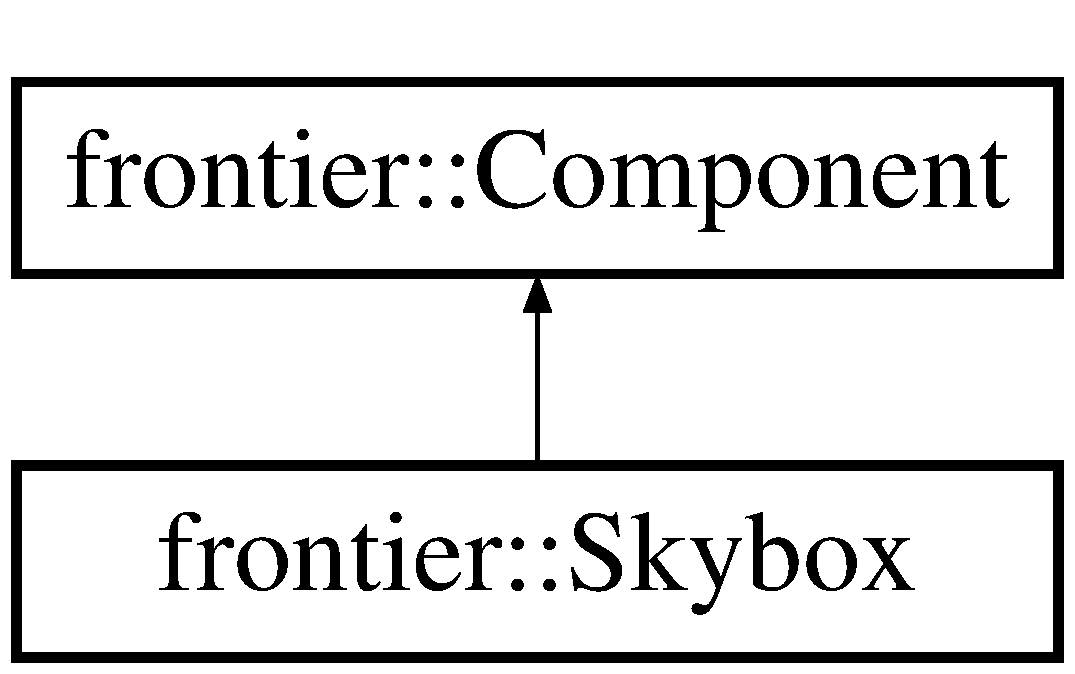
\includegraphics[height=2.000000cm]{classfrontier_1_1_skybox}
\end{center}
\end{figure}
\subsection*{Public Member Functions}
\begin{DoxyCompactItemize}
\item 
void \hyperlink{classfrontier_1_1_skybox_a02a06c87053a2efd6893c0b07465f3c2}{On\+Init} (std\+::weak\+\_\+ptr$<$ \hyperlink{classfrontier_1_1_entity}{Entity} $>$ \+\_\+parent, std\+::shared\+\_\+ptr$<$ \hyperlink{classfrontier_1_1_cubemap_texture}{Cubemap\+Texture} $>$ \+\_\+skybox\+Texture)
\item 
void \hyperlink{classfrontier_1_1_skybox_a38b2ec1a28314c901f4388745d8f0471}{On\+Tick} () override
\end{DoxyCompactItemize}
\subsection*{Additional Inherited Members}


\subsection{Member Function Documentation}
\mbox{\Hypertarget{classfrontier_1_1_skybox_a02a06c87053a2efd6893c0b07465f3c2}\label{classfrontier_1_1_skybox_a02a06c87053a2efd6893c0b07465f3c2}} 
\index{frontier\+::\+Skybox@{frontier\+::\+Skybox}!On\+Init@{On\+Init}}
\index{On\+Init@{On\+Init}!frontier\+::\+Skybox@{frontier\+::\+Skybox}}
\subsubsection{\texorpdfstring{On\+Init()}{OnInit()}}
{\footnotesize\ttfamily void frontier\+::\+Skybox\+::\+On\+Init (\begin{DoxyParamCaption}\item[{std\+::weak\+\_\+ptr$<$ \hyperlink{classfrontier_1_1_entity}{Entity} $>$}]{\+\_\+parent,  }\item[{std\+::shared\+\_\+ptr$<$ \hyperlink{classfrontier_1_1_cubemap_texture}{Cubemap\+Texture} $>$}]{\+\_\+skybox\+Texture }\end{DoxyParamCaption})}

\mbox{\Hypertarget{classfrontier_1_1_skybox_a38b2ec1a28314c901f4388745d8f0471}\label{classfrontier_1_1_skybox_a38b2ec1a28314c901f4388745d8f0471}} 
\index{frontier\+::\+Skybox@{frontier\+::\+Skybox}!On\+Tick@{On\+Tick}}
\index{On\+Tick@{On\+Tick}!frontier\+::\+Skybox@{frontier\+::\+Skybox}}
\subsubsection{\texorpdfstring{On\+Tick()}{OnTick()}}
{\footnotesize\ttfamily void frontier\+::\+Skybox\+::\+On\+Tick (\begin{DoxyParamCaption}{ }\end{DoxyParamCaption})\hspace{0.3cm}{\ttfamily [override]}, {\ttfamily [virtual]}}



Reimplemented from \hyperlink{classfrontier_1_1_component_ab920f9bc07ce051ebb5559c5a66508d1}{frontier\+::\+Component}.



The documentation for this class was generated from the following files\+:\begin{DoxyCompactItemize}
\item 
src/myengine/\hyperlink{_skybox_8h}{Skybox.\+h}\item 
src/myengine/\hyperlink{_skybox_8cpp}{Skybox.\+cpp}\end{DoxyCompactItemize}

\hypertarget{classfrontier_1_1_sound}{}\section{frontier\+:\+:Sound Class Reference}
\label{classfrontier_1_1_sound}\index{frontier\+::\+Sound@{frontier\+::\+Sound}}


Container for a sound. Uses Open\+AL.  




{\ttfamily \#include $<$Sound.\+h$>$}

Inheritance diagram for frontier\+:\+:Sound\+:\begin{figure}[H]
\begin{center}
\leavevmode
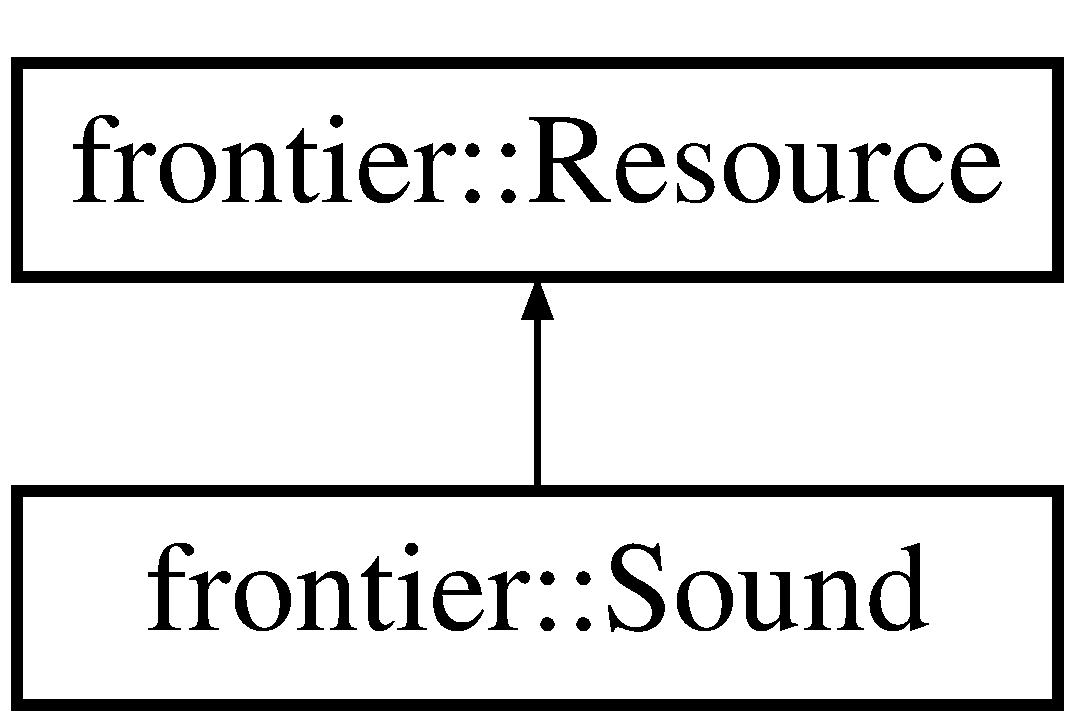
\includegraphics[height=2.000000cm]{classfrontier_1_1_sound}
\end{center}
\end{figure}
\subsection*{Public Member Functions}
\begin{DoxyCompactItemize}
\item 
void \hyperlink{classfrontier_1_1_sound_a9a34b2a30c3eb91702b07c35de9d140b}{Load} (std\+::string \+\_\+path)
\begin{DoxyCompactList}\small\item\em Loads the sound file from a filepath. \end{DoxyCompactList}\item 
void \hyperlink{classfrontier_1_1_sound_a10dbe1366c8069e71e4d3d9f3d8def59}{Play} (float \+\_\+vol, float \+\_\+var\+Min, float \+\_\+var\+Max, glm\+::vec3 \+\_\+sound\+Position=glm\+::vec3(0.\+0f, 0.\+0f, 0.\+0f), glm\+::vec3 \+\_\+listener\+Position=glm\+::vec3(0.\+0f, 0.\+0f, 0.\+0f))
\begin{DoxyCompactList}\small\item\em Plays the sound with a pitch shift. \end{DoxyCompactList}\item 
void \hyperlink{classfrontier_1_1_sound_ae3a9579cf18de757f4bfb02ebf7c688f}{Play} (glm\+::vec3 \+\_\+sound\+Position=glm\+::vec3(0.\+0f, 0.\+0f, 0.\+0f), glm\+::vec3 \+\_\+listener\+Position=glm\+::vec3(0.\+0f, 0.\+0f, 0.\+0f), bool \+\_\+looping=false)
\begin{DoxyCompactList}\small\item\em Plays the sound. \end{DoxyCompactList}\item 
void \hyperlink{classfrontier_1_1_sound_abece17f8675b311e509c969254411c73}{Stop} ()
\begin{DoxyCompactList}\small\item\em Stops playing the sound if it is already playing. \end{DoxyCompactList}\end{DoxyCompactItemize}
\subsection*{Static Public Member Functions}
\begin{DoxyCompactItemize}
\item 
static std\+::shared\+\_\+ptr$<$ \hyperlink{classfrontier_1_1_sound}{Sound} $>$ \hyperlink{classfrontier_1_1_sound_af5b4d6b995926f68fe4219b144046093}{Create} (std\+::string \+\_\+path, std\+::shared\+\_\+ptr$<$ \hyperlink{classfrontier_1_1_resources}{Resources} $>$ \+\_\+resources)
\begin{DoxyCompactList}\small\item\em Creates a sound from an ogg file. \end{DoxyCompactList}\end{DoxyCompactItemize}


\subsection{Detailed Description}
Container for a sound. Uses Open\+AL. 

\subsection{Member Function Documentation}
\mbox{\Hypertarget{classfrontier_1_1_sound_af5b4d6b995926f68fe4219b144046093}\label{classfrontier_1_1_sound_af5b4d6b995926f68fe4219b144046093}} 
\index{frontier\+::\+Sound@{frontier\+::\+Sound}!Create@{Create}}
\index{Create@{Create}!frontier\+::\+Sound@{frontier\+::\+Sound}}
\subsubsection{\texorpdfstring{Create()}{Create()}}
{\footnotesize\ttfamily std\+::shared\+\_\+ptr$<$ \hyperlink{classfrontier_1_1_sound}{Sound} $>$ frontier\+::\+Sound\+::\+Create (\begin{DoxyParamCaption}\item[{std\+::string}]{\+\_\+path,  }\item[{std\+::shared\+\_\+ptr$<$ \hyperlink{classfrontier_1_1_resources}{Resources} $>$}]{\+\_\+resources }\end{DoxyParamCaption})\hspace{0.3cm}{\ttfamily [static]}}



Creates a sound from an ogg file. 


\begin{DoxyParams}{Parameters}
{\em \+\_\+path} & The filepath for the sound. \\
\hline
{\em \+\_\+resources} & A pointer to the resources file. \\
\hline
\end{DoxyParams}
\mbox{\Hypertarget{classfrontier_1_1_sound_a9a34b2a30c3eb91702b07c35de9d140b}\label{classfrontier_1_1_sound_a9a34b2a30c3eb91702b07c35de9d140b}} 
\index{frontier\+::\+Sound@{frontier\+::\+Sound}!Load@{Load}}
\index{Load@{Load}!frontier\+::\+Sound@{frontier\+::\+Sound}}
\subsubsection{\texorpdfstring{Load()}{Load()}}
{\footnotesize\ttfamily void frontier\+::\+Sound\+::\+Load (\begin{DoxyParamCaption}\item[{std\+::string}]{\+\_\+path }\end{DoxyParamCaption})}



Loads the sound file from a filepath. 


\begin{DoxyParams}{Parameters}
{\em \+\_\+path} & The filepath for the sound. \\
\hline
\end{DoxyParams}
\mbox{\Hypertarget{classfrontier_1_1_sound_a10dbe1366c8069e71e4d3d9f3d8def59}\label{classfrontier_1_1_sound_a10dbe1366c8069e71e4d3d9f3d8def59}} 
\index{frontier\+::\+Sound@{frontier\+::\+Sound}!Play@{Play}}
\index{Play@{Play}!frontier\+::\+Sound@{frontier\+::\+Sound}}
\subsubsection{\texorpdfstring{Play()}{Play()}\hspace{0.1cm}{\footnotesize\ttfamily [1/2]}}
{\footnotesize\ttfamily void frontier\+::\+Sound\+::\+Play (\begin{DoxyParamCaption}\item[{float}]{\+\_\+vol,  }\item[{float}]{\+\_\+var\+Min,  }\item[{float}]{\+\_\+var\+Max,  }\item[{glm\+::vec3}]{\+\_\+sound\+Position = {\ttfamily glm\+:\+:vec3(0.0f,~0.0f,~0.0f)},  }\item[{glm\+::vec3}]{\+\_\+listener\+Position = {\ttfamily glm\+:\+:vec3(0.0f,~0.0f,~0.0f)} }\end{DoxyParamCaption})}



Plays the sound with a pitch shift. 


\begin{DoxyParams}{Parameters}
{\em \+\_\+vol} & The volume of the sound when playing. \\
\hline
{\em \+\_\+var\+Min} & The minimum pitch of the sound. \\
\hline
{\em \+\_\+var\+Max} & The maximum pitch of the sound. \\
\hline
{\em \+\_\+sound\+Position} & The position of the sound. \\
\hline
{\em \+\_\+listener\+Position} & The position of the listener. \\
\hline
\end{DoxyParams}
\mbox{\Hypertarget{classfrontier_1_1_sound_ae3a9579cf18de757f4bfb02ebf7c688f}\label{classfrontier_1_1_sound_ae3a9579cf18de757f4bfb02ebf7c688f}} 
\index{frontier\+::\+Sound@{frontier\+::\+Sound}!Play@{Play}}
\index{Play@{Play}!frontier\+::\+Sound@{frontier\+::\+Sound}}
\subsubsection{\texorpdfstring{Play()}{Play()}\hspace{0.1cm}{\footnotesize\ttfamily [2/2]}}
{\footnotesize\ttfamily void frontier\+::\+Sound\+::\+Play (\begin{DoxyParamCaption}\item[{glm\+::vec3}]{\+\_\+sound\+Position = {\ttfamily glm\+:\+:vec3(0.0f,~0.0f,~0.0f)},  }\item[{glm\+::vec3}]{\+\_\+listener\+Position = {\ttfamily glm\+:\+:vec3(0.0f,~0.0f,~0.0f)},  }\item[{bool}]{\+\_\+looping = {\ttfamily false} }\end{DoxyParamCaption})}



Plays the sound. 


\begin{DoxyParams}{Parameters}
{\em \+\_\+sound\+Position} & The position of the sound. \\
\hline
{\em \+\_\+listener\+Position} & The position of the listener. \\
\hline
{\em \+\_\+looping} & Whether the sound should loop. \\
\hline
\end{DoxyParams}
\mbox{\Hypertarget{classfrontier_1_1_sound_abece17f8675b311e509c969254411c73}\label{classfrontier_1_1_sound_abece17f8675b311e509c969254411c73}} 
\index{frontier\+::\+Sound@{frontier\+::\+Sound}!Stop@{Stop}}
\index{Stop@{Stop}!frontier\+::\+Sound@{frontier\+::\+Sound}}
\subsubsection{\texorpdfstring{Stop()}{Stop()}}
{\footnotesize\ttfamily void frontier\+::\+Sound\+::\+Stop (\begin{DoxyParamCaption}{ }\end{DoxyParamCaption})}



Stops playing the sound if it is already playing. 



The documentation for this class was generated from the following files\+:\begin{DoxyCompactItemize}
\item 
src/myengine/\hyperlink{_sound_8h}{Sound.\+h}\item 
src/myengine/\hyperlink{_sound_8cpp}{Sound.\+cpp}\end{DoxyCompactItemize}

\hypertarget{structfrontier_1_1_sound_impl}{}\section{frontier\+:\+:Sound\+Impl Struct Reference}
\label{structfrontier_1_1_sound_impl}\index{frontier\+::\+Sound\+Impl@{frontier\+::\+Sound\+Impl}}
\subsection*{Public Member Functions}
\begin{DoxyCompactItemize}
\item 
\hyperlink{structfrontier_1_1_sound_impl_af5689c9a50ec077e5f29747db97015b9}{$\sim$\+Sound\+Impl} ()
\item 
void \hyperlink{structfrontier_1_1_sound_impl_aa7170ec2e5d847deda459543a38670e0}{load\+\_\+ogg} (std\+::string \+\_\+file\+Name, std\+::vector$<$ char $>$ \&\+\_\+buffer, A\+Lenum \&\+\_\+format, A\+Lsizei \&\+\_\+freq)
\end{DoxyCompactItemize}
\subsection*{Public Attributes}
\begin{DoxyCompactItemize}
\item 
A\+Luint \hyperlink{structfrontier_1_1_sound_impl_ae8b2e75a8ca0784b44f0e167d69a1128}{id}
\end{DoxyCompactItemize}


\subsection{Constructor \& Destructor Documentation}
\mbox{\Hypertarget{structfrontier_1_1_sound_impl_af5689c9a50ec077e5f29747db97015b9}\label{structfrontier_1_1_sound_impl_af5689c9a50ec077e5f29747db97015b9}} 
\index{frontier\+::\+Sound\+Impl@{frontier\+::\+Sound\+Impl}!````~Sound\+Impl@{$\sim$\+Sound\+Impl}}
\index{````~Sound\+Impl@{$\sim$\+Sound\+Impl}!frontier\+::\+Sound\+Impl@{frontier\+::\+Sound\+Impl}}
\subsubsection{\texorpdfstring{$\sim$\+Sound\+Impl()}{~SoundImpl()}}
{\footnotesize\ttfamily frontier\+::\+Sound\+Impl\+::$\sim$\+Sound\+Impl (\begin{DoxyParamCaption}{ }\end{DoxyParamCaption})\hspace{0.3cm}{\ttfamily [inline]}}



\subsection{Member Function Documentation}
\mbox{\Hypertarget{structfrontier_1_1_sound_impl_aa7170ec2e5d847deda459543a38670e0}\label{structfrontier_1_1_sound_impl_aa7170ec2e5d847deda459543a38670e0}} 
\index{frontier\+::\+Sound\+Impl@{frontier\+::\+Sound\+Impl}!load\+\_\+ogg@{load\+\_\+ogg}}
\index{load\+\_\+ogg@{load\+\_\+ogg}!frontier\+::\+Sound\+Impl@{frontier\+::\+Sound\+Impl}}
\subsubsection{\texorpdfstring{load\+\_\+ogg()}{load\_ogg()}}
{\footnotesize\ttfamily void frontier\+::\+Sound\+Impl\+::load\+\_\+ogg (\begin{DoxyParamCaption}\item[{std\+::string}]{\+\_\+file\+Name,  }\item[{std\+::vector$<$ char $>$ \&}]{\+\_\+buffer,  }\item[{A\+Lenum \&}]{\+\_\+format,  }\item[{A\+Lsizei \&}]{\+\_\+freq }\end{DoxyParamCaption})\hspace{0.3cm}{\ttfamily [inline]}}



\subsection{Member Data Documentation}
\mbox{\Hypertarget{structfrontier_1_1_sound_impl_ae8b2e75a8ca0784b44f0e167d69a1128}\label{structfrontier_1_1_sound_impl_ae8b2e75a8ca0784b44f0e167d69a1128}} 
\index{frontier\+::\+Sound\+Impl@{frontier\+::\+Sound\+Impl}!id@{id}}
\index{id@{id}!frontier\+::\+Sound\+Impl@{frontier\+::\+Sound\+Impl}}
\subsubsection{\texorpdfstring{id}{id}}
{\footnotesize\ttfamily A\+Luint frontier\+::\+Sound\+Impl\+::id}



The documentation for this struct was generated from the following file\+:\begin{DoxyCompactItemize}
\item 
src/myengine/\hyperlink{_sound_8cpp}{Sound.\+cpp}\end{DoxyCompactItemize}

\hypertarget{classfrontier_1_1_texture}{}\section{frontier\+:\+:Texture Class Reference}
\label{classfrontier_1_1_texture}\index{frontier\+::\+Texture@{frontier\+::\+Texture}}


A container for an image, loaded externally.  




{\ttfamily \#include $<$Texture.\+h$>$}

Inheritance diagram for frontier\+:\+:Texture\+:\begin{figure}[H]
\begin{center}
\leavevmode
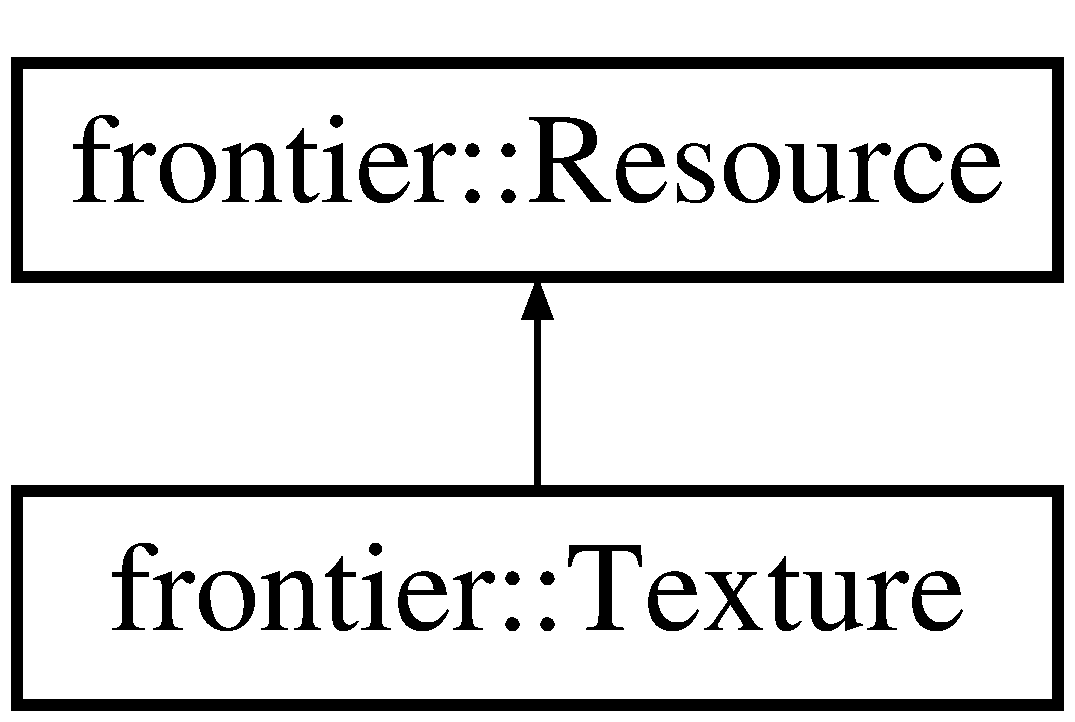
\includegraphics[height=2.000000cm]{classfrontier_1_1_texture}
\end{center}
\end{figure}
\subsection*{Public Member Functions}
\begin{DoxyCompactItemize}
\item 
void \hyperlink{classfrontier_1_1_texture_aa77328fcbb46a524cc7c8bd6b149d3cc}{Set\+Texture} (G\+Luint \+\_\+new\+ID, int \+\_\+texture\+Location)
\begin{DoxyCompactList}\small\item\em Sets a new texture. \end{DoxyCompactList}\item 
G\+Luint \hyperlink{classfrontier_1_1_texture_ac6ca90a251f23a0fcbcf56ae7b3bb544}{Get\+Texture} ()
\begin{DoxyCompactList}\small\item\em Gets the current \hyperlink{classfrontier_1_1_texture}{Texture} ID;. \end{DoxyCompactList}\item 
int \hyperlink{classfrontier_1_1_texture_a93935a9af5c67d31eaf7c8074dbb13c5}{Get\+Texture\+Location} ()
\begin{DoxyCompactList}\small\item\em Gets the current texture location. \end{DoxyCompactList}\item 
void \hyperlink{classfrontier_1_1_texture_ae983ce4ddd78a5170e3beed65b17ae3f}{Bind\+Texture} ()
\begin{DoxyCompactList}\small\item\em Binds the current texture. \end{DoxyCompactList}\item 
void \hyperlink{classfrontier_1_1_texture_a53375bba8b0277c792c64d0246a10fd3}{Set\+Width} (int \+\_\+new\+Width)
\begin{DoxyCompactList}\small\item\em Sets the width of the texture. \end{DoxyCompactList}\item 
void \hyperlink{classfrontier_1_1_texture_aa927deb382a4b19374edc030c76ed1c6}{Set\+Height} (int \+\_\+new\+Height)
\begin{DoxyCompactList}\small\item\em Sets the height of the texture. \end{DoxyCompactList}\item 
int \hyperlink{classfrontier_1_1_texture_acd83cfddc6017cf76ccc37294a9c38be}{Get\+Width} ()
\begin{DoxyCompactList}\small\item\em Gets the current width of the texture. \end{DoxyCompactList}\item 
int \hyperlink{classfrontier_1_1_texture_a55c5dc9f91d6d06abf32955de24290ae}{Get\+Height} ()
\begin{DoxyCompactList}\small\item\em Gets the current height of the texture. \end{DoxyCompactList}\end{DoxyCompactItemize}
\subsection*{Static Public Member Functions}
\begin{DoxyCompactItemize}
\item 
static std\+::shared\+\_\+ptr$<$ \hyperlink{classfrontier_1_1_texture}{Texture} $>$ \hyperlink{classfrontier_1_1_texture_a52eabdae7b6d59bdc14cde2e4ae95f26}{Create} (const char $\ast$\+\_\+path, std\+::shared\+\_\+ptr$<$ \hyperlink{classfrontier_1_1_resources}{Resources} $>$ \+\_\+resources, int \+\_\+texture\+Location)
\begin{DoxyCompactList}\small\item\em Creates the image. \end{DoxyCompactList}\end{DoxyCompactItemize}


\subsection{Detailed Description}
A container for an image, loaded externally. 

\subsection{Member Function Documentation}
\mbox{\Hypertarget{classfrontier_1_1_texture_ae983ce4ddd78a5170e3beed65b17ae3f}\label{classfrontier_1_1_texture_ae983ce4ddd78a5170e3beed65b17ae3f}} 
\index{frontier\+::\+Texture@{frontier\+::\+Texture}!Bind\+Texture@{Bind\+Texture}}
\index{Bind\+Texture@{Bind\+Texture}!frontier\+::\+Texture@{frontier\+::\+Texture}}
\subsubsection{\texorpdfstring{Bind\+Texture()}{BindTexture()}}
{\footnotesize\ttfamily void frontier\+::\+Texture\+::\+Bind\+Texture (\begin{DoxyParamCaption}{ }\end{DoxyParamCaption})}



Binds the current texture. 

\mbox{\Hypertarget{classfrontier_1_1_texture_a52eabdae7b6d59bdc14cde2e4ae95f26}\label{classfrontier_1_1_texture_a52eabdae7b6d59bdc14cde2e4ae95f26}} 
\index{frontier\+::\+Texture@{frontier\+::\+Texture}!Create@{Create}}
\index{Create@{Create}!frontier\+::\+Texture@{frontier\+::\+Texture}}
\subsubsection{\texorpdfstring{Create()}{Create()}}
{\footnotesize\ttfamily std\+::shared\+\_\+ptr$<$ \hyperlink{classfrontier_1_1_texture}{Texture} $>$ frontier\+::\+Texture\+::\+Create (\begin{DoxyParamCaption}\item[{const char $\ast$}]{\+\_\+path,  }\item[{std\+::shared\+\_\+ptr$<$ \hyperlink{classfrontier_1_1_resources}{Resources} $>$}]{\+\_\+resources,  }\item[{int}]{\+\_\+texture\+Location }\end{DoxyParamCaption})\hspace{0.3cm}{\ttfamily [static]}}



Creates the image. 


\begin{DoxyParams}{Parameters}
{\em \+\_\+path} & The filepath for the image. \\
\hline
{\em \+\_\+resources} & Pointer to the resources class. \\
\hline
{\em \+\_\+texture\+Location} & The location where the texture will be located on the G\+PU. \\
\hline
\end{DoxyParams}
\mbox{\Hypertarget{classfrontier_1_1_texture_a55c5dc9f91d6d06abf32955de24290ae}\label{classfrontier_1_1_texture_a55c5dc9f91d6d06abf32955de24290ae}} 
\index{frontier\+::\+Texture@{frontier\+::\+Texture}!Get\+Height@{Get\+Height}}
\index{Get\+Height@{Get\+Height}!frontier\+::\+Texture@{frontier\+::\+Texture}}
\subsubsection{\texorpdfstring{Get\+Height()}{GetHeight()}}
{\footnotesize\ttfamily int frontier\+::\+Texture\+::\+Get\+Height (\begin{DoxyParamCaption}{ }\end{DoxyParamCaption})}



Gets the current height of the texture. 

\mbox{\Hypertarget{classfrontier_1_1_texture_ac6ca90a251f23a0fcbcf56ae7b3bb544}\label{classfrontier_1_1_texture_ac6ca90a251f23a0fcbcf56ae7b3bb544}} 
\index{frontier\+::\+Texture@{frontier\+::\+Texture}!Get\+Texture@{Get\+Texture}}
\index{Get\+Texture@{Get\+Texture}!frontier\+::\+Texture@{frontier\+::\+Texture}}
\subsubsection{\texorpdfstring{Get\+Texture()}{GetTexture()}}
{\footnotesize\ttfamily G\+Luint frontier\+::\+Texture\+::\+Get\+Texture (\begin{DoxyParamCaption}{ }\end{DoxyParamCaption})}



Gets the current \hyperlink{classfrontier_1_1_texture}{Texture} ID;. 

\mbox{\Hypertarget{classfrontier_1_1_texture_a93935a9af5c67d31eaf7c8074dbb13c5}\label{classfrontier_1_1_texture_a93935a9af5c67d31eaf7c8074dbb13c5}} 
\index{frontier\+::\+Texture@{frontier\+::\+Texture}!Get\+Texture\+Location@{Get\+Texture\+Location}}
\index{Get\+Texture\+Location@{Get\+Texture\+Location}!frontier\+::\+Texture@{frontier\+::\+Texture}}
\subsubsection{\texorpdfstring{Get\+Texture\+Location()}{GetTextureLocation()}}
{\footnotesize\ttfamily int frontier\+::\+Texture\+::\+Get\+Texture\+Location (\begin{DoxyParamCaption}{ }\end{DoxyParamCaption})}



Gets the current texture location. 

\mbox{\Hypertarget{classfrontier_1_1_texture_acd83cfddc6017cf76ccc37294a9c38be}\label{classfrontier_1_1_texture_acd83cfddc6017cf76ccc37294a9c38be}} 
\index{frontier\+::\+Texture@{frontier\+::\+Texture}!Get\+Width@{Get\+Width}}
\index{Get\+Width@{Get\+Width}!frontier\+::\+Texture@{frontier\+::\+Texture}}
\subsubsection{\texorpdfstring{Get\+Width()}{GetWidth()}}
{\footnotesize\ttfamily int frontier\+::\+Texture\+::\+Get\+Width (\begin{DoxyParamCaption}{ }\end{DoxyParamCaption})}



Gets the current width of the texture. 

\mbox{\Hypertarget{classfrontier_1_1_texture_aa927deb382a4b19374edc030c76ed1c6}\label{classfrontier_1_1_texture_aa927deb382a4b19374edc030c76ed1c6}} 
\index{frontier\+::\+Texture@{frontier\+::\+Texture}!Set\+Height@{Set\+Height}}
\index{Set\+Height@{Set\+Height}!frontier\+::\+Texture@{frontier\+::\+Texture}}
\subsubsection{\texorpdfstring{Set\+Height()}{SetHeight()}}
{\footnotesize\ttfamily void frontier\+::\+Texture\+::\+Set\+Height (\begin{DoxyParamCaption}\item[{int}]{\+\_\+new\+Height }\end{DoxyParamCaption})}



Sets the height of the texture. 


\begin{DoxyParams}{Parameters}
{\em \+\_\+new\+Width} & The new height of the texture. \\
\hline
\end{DoxyParams}
\mbox{\Hypertarget{classfrontier_1_1_texture_aa77328fcbb46a524cc7c8bd6b149d3cc}\label{classfrontier_1_1_texture_aa77328fcbb46a524cc7c8bd6b149d3cc}} 
\index{frontier\+::\+Texture@{frontier\+::\+Texture}!Set\+Texture@{Set\+Texture}}
\index{Set\+Texture@{Set\+Texture}!frontier\+::\+Texture@{frontier\+::\+Texture}}
\subsubsection{\texorpdfstring{Set\+Texture()}{SetTexture()}}
{\footnotesize\ttfamily void frontier\+::\+Texture\+::\+Set\+Texture (\begin{DoxyParamCaption}\item[{G\+Luint}]{\+\_\+new\+ID,  }\item[{int}]{\+\_\+texture\+Location }\end{DoxyParamCaption})}



Sets a new texture. 


\begin{DoxyParams}{Parameters}
{\em \+\_\+new\+ID} & The new ID for the texture. \\
\hline
{\em \+\_\+texture\+Location} & The location where the texture will be located on the G\+PU. \\
\hline
\end{DoxyParams}
\mbox{\Hypertarget{classfrontier_1_1_texture_a53375bba8b0277c792c64d0246a10fd3}\label{classfrontier_1_1_texture_a53375bba8b0277c792c64d0246a10fd3}} 
\index{frontier\+::\+Texture@{frontier\+::\+Texture}!Set\+Width@{Set\+Width}}
\index{Set\+Width@{Set\+Width}!frontier\+::\+Texture@{frontier\+::\+Texture}}
\subsubsection{\texorpdfstring{Set\+Width()}{SetWidth()}}
{\footnotesize\ttfamily void frontier\+::\+Texture\+::\+Set\+Width (\begin{DoxyParamCaption}\item[{int}]{\+\_\+new\+Width }\end{DoxyParamCaption})}



Sets the width of the texture. 


\begin{DoxyParams}{Parameters}
{\em \+\_\+new\+Width} & The new width of the texture. \\
\hline
\end{DoxyParams}


The documentation for this class was generated from the following files\+:\begin{DoxyCompactItemize}
\item 
src/myengine/\hyperlink{_texture_8h}{Texture.\+h}\item 
src/myengine/\hyperlink{_texture_8cpp}{Texture.\+cpp}\end{DoxyCompactItemize}

\hypertarget{classfrontier_1_1_timer}{}\section{frontier\+:\+:Timer Class Reference}
\label{classfrontier_1_1_timer}\index{frontier\+::\+Timer@{frontier\+::\+Timer}}


{\ttfamily \#include $<$Timer.\+h$>$}

\subsection*{Public Member Functions}
\begin{DoxyCompactItemize}
\item 
\hyperlink{classfrontier_1_1_timer_a6aac1ba4a567320f54e8eee841e9c43b}{Timer} ()
\item 
void \hyperlink{classfrontier_1_1_timer_a26c5d9aeddfcb91bea46d7f14b35e923}{Start} ()
\item 
void \hyperlink{classfrontier_1_1_timer_a878f61e350e7bb28350964f105192533}{Stop} ()
\item 
void \hyperlink{classfrontier_1_1_timer_a9d4c0d3d515cea7b5784ca7488b01d79}{Pause} ()
\item 
void \hyperlink{classfrontier_1_1_timer_a18d0b8d623b50b64fb0893cd9dec56ce}{Unpause} ()
\item 
Uint32 \hyperlink{classfrontier_1_1_timer_ac34abf0e1fada4f0b1f97087c6b6747f}{Get\+Ticks} ()
\item 
bool \hyperlink{classfrontier_1_1_timer_a955bac73463eb53813b84c945f0b9327}{Is\+Started} ()
\item 
bool \hyperlink{classfrontier_1_1_timer_ab1436c1f41e9226977fc8500b6fe3b41}{Is\+Paused} ()
\end{DoxyCompactItemize}


\subsection{Constructor \& Destructor Documentation}
\mbox{\Hypertarget{classfrontier_1_1_timer_a6aac1ba4a567320f54e8eee841e9c43b}\label{classfrontier_1_1_timer_a6aac1ba4a567320f54e8eee841e9c43b}} 
\index{frontier\+::\+Timer@{frontier\+::\+Timer}!Timer@{Timer}}
\index{Timer@{Timer}!frontier\+::\+Timer@{frontier\+::\+Timer}}
\subsubsection{\texorpdfstring{Timer()}{Timer()}}
{\footnotesize\ttfamily frontier\+::\+Timer\+::\+Timer (\begin{DoxyParamCaption}{ }\end{DoxyParamCaption})}



\subsection{Member Function Documentation}
\mbox{\Hypertarget{classfrontier_1_1_timer_ac34abf0e1fada4f0b1f97087c6b6747f}\label{classfrontier_1_1_timer_ac34abf0e1fada4f0b1f97087c6b6747f}} 
\index{frontier\+::\+Timer@{frontier\+::\+Timer}!Get\+Ticks@{Get\+Ticks}}
\index{Get\+Ticks@{Get\+Ticks}!frontier\+::\+Timer@{frontier\+::\+Timer}}
\subsubsection{\texorpdfstring{Get\+Ticks()}{GetTicks()}}
{\footnotesize\ttfamily Uint32 frontier\+::\+Timer\+::\+Get\+Ticks (\begin{DoxyParamCaption}{ }\end{DoxyParamCaption})}

\mbox{\Hypertarget{classfrontier_1_1_timer_ab1436c1f41e9226977fc8500b6fe3b41}\label{classfrontier_1_1_timer_ab1436c1f41e9226977fc8500b6fe3b41}} 
\index{frontier\+::\+Timer@{frontier\+::\+Timer}!Is\+Paused@{Is\+Paused}}
\index{Is\+Paused@{Is\+Paused}!frontier\+::\+Timer@{frontier\+::\+Timer}}
\subsubsection{\texorpdfstring{Is\+Paused()}{IsPaused()}}
{\footnotesize\ttfamily bool frontier\+::\+Timer\+::\+Is\+Paused (\begin{DoxyParamCaption}{ }\end{DoxyParamCaption})}

\mbox{\Hypertarget{classfrontier_1_1_timer_a955bac73463eb53813b84c945f0b9327}\label{classfrontier_1_1_timer_a955bac73463eb53813b84c945f0b9327}} 
\index{frontier\+::\+Timer@{frontier\+::\+Timer}!Is\+Started@{Is\+Started}}
\index{Is\+Started@{Is\+Started}!frontier\+::\+Timer@{frontier\+::\+Timer}}
\subsubsection{\texorpdfstring{Is\+Started()}{IsStarted()}}
{\footnotesize\ttfamily bool frontier\+::\+Timer\+::\+Is\+Started (\begin{DoxyParamCaption}{ }\end{DoxyParamCaption})}

\mbox{\Hypertarget{classfrontier_1_1_timer_a9d4c0d3d515cea7b5784ca7488b01d79}\label{classfrontier_1_1_timer_a9d4c0d3d515cea7b5784ca7488b01d79}} 
\index{frontier\+::\+Timer@{frontier\+::\+Timer}!Pause@{Pause}}
\index{Pause@{Pause}!frontier\+::\+Timer@{frontier\+::\+Timer}}
\subsubsection{\texorpdfstring{Pause()}{Pause()}}
{\footnotesize\ttfamily void frontier\+::\+Timer\+::\+Pause (\begin{DoxyParamCaption}{ }\end{DoxyParamCaption})}

\mbox{\Hypertarget{classfrontier_1_1_timer_a26c5d9aeddfcb91bea46d7f14b35e923}\label{classfrontier_1_1_timer_a26c5d9aeddfcb91bea46d7f14b35e923}} 
\index{frontier\+::\+Timer@{frontier\+::\+Timer}!Start@{Start}}
\index{Start@{Start}!frontier\+::\+Timer@{frontier\+::\+Timer}}
\subsubsection{\texorpdfstring{Start()}{Start()}}
{\footnotesize\ttfamily void frontier\+::\+Timer\+::\+Start (\begin{DoxyParamCaption}{ }\end{DoxyParamCaption})}

\mbox{\Hypertarget{classfrontier_1_1_timer_a878f61e350e7bb28350964f105192533}\label{classfrontier_1_1_timer_a878f61e350e7bb28350964f105192533}} 
\index{frontier\+::\+Timer@{frontier\+::\+Timer}!Stop@{Stop}}
\index{Stop@{Stop}!frontier\+::\+Timer@{frontier\+::\+Timer}}
\subsubsection{\texorpdfstring{Stop()}{Stop()}}
{\footnotesize\ttfamily void frontier\+::\+Timer\+::\+Stop (\begin{DoxyParamCaption}{ }\end{DoxyParamCaption})}

\mbox{\Hypertarget{classfrontier_1_1_timer_a18d0b8d623b50b64fb0893cd9dec56ce}\label{classfrontier_1_1_timer_a18d0b8d623b50b64fb0893cd9dec56ce}} 
\index{frontier\+::\+Timer@{frontier\+::\+Timer}!Unpause@{Unpause}}
\index{Unpause@{Unpause}!frontier\+::\+Timer@{frontier\+::\+Timer}}
\subsubsection{\texorpdfstring{Unpause()}{Unpause()}}
{\footnotesize\ttfamily void frontier\+::\+Timer\+::\+Unpause (\begin{DoxyParamCaption}{ }\end{DoxyParamCaption})}



The documentation for this class was generated from the following files\+:\begin{DoxyCompactItemize}
\item 
src/myengine/\hyperlink{_timer_8h}{Timer.\+h}\item 
src/myengine/\hyperlink{_timer_8cpp}{Timer.\+cpp}\end{DoxyCompactItemize}

\hypertarget{classfrontier_1_1_transform}{}\section{frontier\+:\+:Transform Class Reference}
\label{classfrontier_1_1_transform}\index{frontier\+::\+Transform@{frontier\+::\+Transform}}


Class that tracks location information on an entity, added by default to an entity on intialisation.  




{\ttfamily \#include $<$Transform.\+h$>$}

Inheritance diagram for frontier\+:\+:Transform\+:\begin{figure}[H]
\begin{center}
\leavevmode
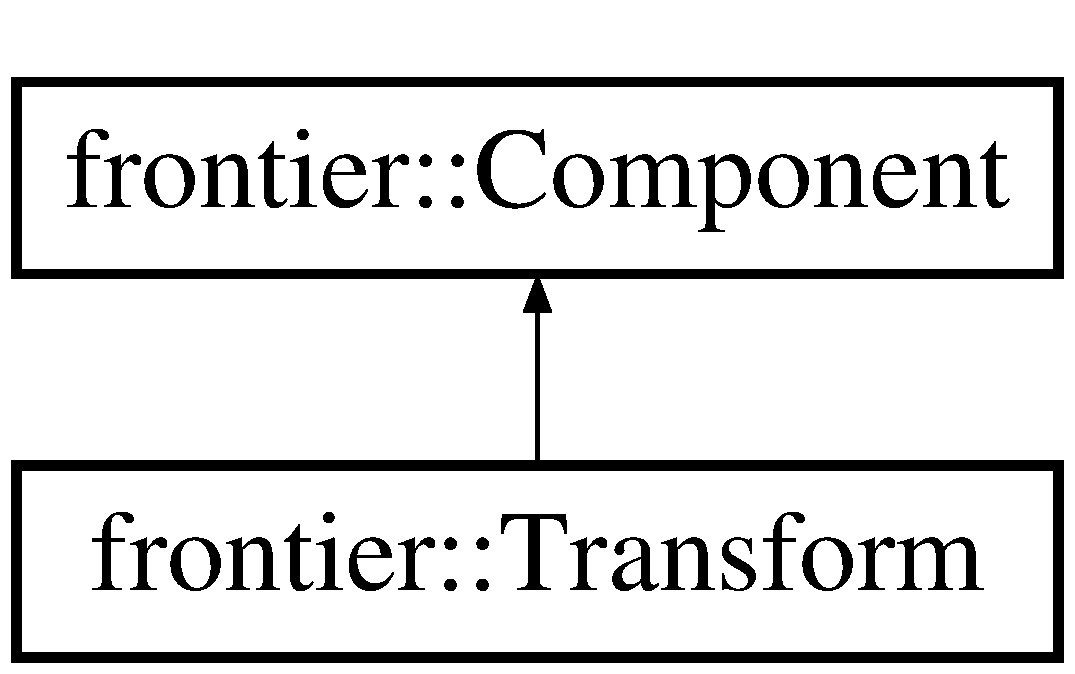
\includegraphics[height=2.000000cm]{classfrontier_1_1_transform}
\end{center}
\end{figure}
\subsection*{Public Member Functions}
\begin{DoxyCompactItemize}
\item 
void \hyperlink{classfrontier_1_1_transform_a2d8181ec0003b04822124340fe7772c0}{On\+Init} (std\+::weak\+\_\+ptr$<$ \hyperlink{classfrontier_1_1_entity}{Entity} $>$ \+\_\+parent) override
\begin{DoxyCompactList}\small\item\em Initialises the transform. \end{DoxyCompactList}\item 
void \hyperlink{classfrontier_1_1_transform_a939611da70fc0f33b85fcf92d101ac3e}{On\+Init} (std\+::weak\+\_\+ptr$<$ \hyperlink{classfrontier_1_1_entity}{Entity} $>$ \+\_\+parent, glm\+::vec3 \+\_\+position)
\begin{DoxyCompactList}\small\item\em Initialises the transform. \end{DoxyCompactList}\item 
void \hyperlink{classfrontier_1_1_transform_ab23c1b75f7a02947bddec97abe286fa3}{On\+Init} (std\+::weak\+\_\+ptr$<$ \hyperlink{classfrontier_1_1_entity}{Entity} $>$ \+\_\+parent, glm\+::vec3 \+\_\+position, glm\+::vec3 \+\_\+rotation)
\begin{DoxyCompactList}\small\item\em Initialises the transform. \end{DoxyCompactList}\item 
void \hyperlink{classfrontier_1_1_transform_a8d2f5d6830818cc167a94948a15b2697}{On\+Init} (std\+::weak\+\_\+ptr$<$ \hyperlink{classfrontier_1_1_entity}{Entity} $>$ \+\_\+parent, glm\+::vec3 \+\_\+position, glm\+::vec3 \+\_\+rotation, glm\+::vec3 \+\_\+scale)
\begin{DoxyCompactList}\small\item\em Initialises the transform. \end{DoxyCompactList}\item 
glm\+::vec3 \hyperlink{classfrontier_1_1_transform_a9807f56b882736521e5678853e8a09c5}{Get\+Position} ()
\begin{DoxyCompactList}\small\item\em Returns the position. \end{DoxyCompactList}\item 
void \hyperlink{classfrontier_1_1_transform_a45f9ecc9db02d813f49211cdd71ec749}{Set\+Position} (glm\+::vec3 \+\_\+pos)
\begin{DoxyCompactList}\small\item\em Sets the position. \end{DoxyCompactList}\item 
glm\+::vec3 \hyperlink{classfrontier_1_1_transform_a1be9d719815ece4e26513567ef2ac23b}{Get\+Rotation} ()
\begin{DoxyCompactList}\small\item\em Returns the rotation. \end{DoxyCompactList}\item 
void \hyperlink{classfrontier_1_1_transform_a62ed231d2cfef5b115955741ec838591}{Set\+Rotation} (glm\+::vec3 \+\_\+rot)
\begin{DoxyCompactList}\small\item\em Sets the rotation. \end{DoxyCompactList}\item 
glm\+::vec3 \hyperlink{classfrontier_1_1_transform_ab3468e4e7603e07e2a1d305c15fc4fd2}{Get\+Scale} ()
\begin{DoxyCompactList}\small\item\em Returns the scale. \end{DoxyCompactList}\item 
void \hyperlink{classfrontier_1_1_transform_ab6803171399b1ba2825f3f47f6eaffaa}{Set\+Scale} (glm\+::vec3 \+\_\+sca)
\begin{DoxyCompactList}\small\item\em Sets the scale. \end{DoxyCompactList}\item 
glm\+::mat4 \hyperlink{classfrontier_1_1_transform_a092823a36448cf201cc63e3cd46d6cc4}{Get\+Model\+Matrix} ()
\begin{DoxyCompactList}\small\item\em Returns the model matrix. \end{DoxyCompactList}\item 
glm\+::mat4 \hyperlink{classfrontier_1_1_transform_aad5a62d25417a16ad84d6f809eebc8fe}{Get\+Model\+Matrix\+Mod\+Scale} (glm\+::vec3 \+\_\+scale\+Modifier)
\begin{DoxyCompactList}\small\item\em Returns the model matrix with a modified scale. \end{DoxyCompactList}\item 
glm\+::mat4 \hyperlink{classfrontier_1_1_transform_ab6bff40a457322589a7f8a1dc92a5c42}{Get\+Position\+Matrix} (int \+\_\+exclude\+Axis=0)
\begin{DoxyCompactList}\small\item\em Returns a model matrix with just the position. \end{DoxyCompactList}\item 
void \hyperlink{classfrontier_1_1_transform_a95b6b6407a5ece2e6b188c2e1c2294a2}{Set\+Transform\+Parent} (std\+::weak\+\_\+ptr$<$ \hyperlink{classfrontier_1_1_transform}{Transform} $>$ \+\_\+parent)
\begin{DoxyCompactList}\small\item\em Sets the transform parent, this is used for scene graphs. \end{DoxyCompactList}\item 
void \hyperlink{classfrontier_1_1_transform_a61510be91275313808daa938af87f119}{Add\+Child} (std\+::weak\+\_\+ptr$<$ \hyperlink{classfrontier_1_1_transform}{Transform} $>$ \+\_\+child)
\begin{DoxyCompactList}\small\item\em adds a child to the transform. \end{DoxyCompactList}\item 
void \hyperlink{classfrontier_1_1_transform_a10e72a1e49de0c3c3a36f920612a39ce}{Set\+Self} (std\+::weak\+\_\+ptr$<$ \hyperlink{classfrontier_1_1_transform}{Transform} $>$ \+\_\+self)
\begin{DoxyCompactList}\small\item\em Sets the self pointer. \end{DoxyCompactList}\end{DoxyCompactItemize}
\subsection*{Additional Inherited Members}


\subsection{Detailed Description}
Class that tracks location information on an entity, added by default to an entity on intialisation. 

\subsection{Member Function Documentation}
\mbox{\Hypertarget{classfrontier_1_1_transform_a61510be91275313808daa938af87f119}\label{classfrontier_1_1_transform_a61510be91275313808daa938af87f119}} 
\index{frontier\+::\+Transform@{frontier\+::\+Transform}!Add\+Child@{Add\+Child}}
\index{Add\+Child@{Add\+Child}!frontier\+::\+Transform@{frontier\+::\+Transform}}
\subsubsection{\texorpdfstring{Add\+Child()}{AddChild()}}
{\footnotesize\ttfamily void frontier\+::\+Transform\+::\+Add\+Child (\begin{DoxyParamCaption}\item[{std\+::weak\+\_\+ptr$<$ \hyperlink{classfrontier_1_1_transform}{Transform} $>$}]{\+\_\+child }\end{DoxyParamCaption})}



adds a child to the transform. 


\begin{DoxyParams}{Parameters}
{\em \+\_\+child} & The new child for this transform. \\
\hline
\end{DoxyParams}
\mbox{\Hypertarget{classfrontier_1_1_transform_a092823a36448cf201cc63e3cd46d6cc4}\label{classfrontier_1_1_transform_a092823a36448cf201cc63e3cd46d6cc4}} 
\index{frontier\+::\+Transform@{frontier\+::\+Transform}!Get\+Model\+Matrix@{Get\+Model\+Matrix}}
\index{Get\+Model\+Matrix@{Get\+Model\+Matrix}!frontier\+::\+Transform@{frontier\+::\+Transform}}
\subsubsection{\texorpdfstring{Get\+Model\+Matrix()}{GetModelMatrix()}}
{\footnotesize\ttfamily glm\+::mat4 frontier\+::\+Transform\+::\+Get\+Model\+Matrix (\begin{DoxyParamCaption}{ }\end{DoxyParamCaption})}



Returns the model matrix. 

\mbox{\Hypertarget{classfrontier_1_1_transform_aad5a62d25417a16ad84d6f809eebc8fe}\label{classfrontier_1_1_transform_aad5a62d25417a16ad84d6f809eebc8fe}} 
\index{frontier\+::\+Transform@{frontier\+::\+Transform}!Get\+Model\+Matrix\+Mod\+Scale@{Get\+Model\+Matrix\+Mod\+Scale}}
\index{Get\+Model\+Matrix\+Mod\+Scale@{Get\+Model\+Matrix\+Mod\+Scale}!frontier\+::\+Transform@{frontier\+::\+Transform}}
\subsubsection{\texorpdfstring{Get\+Model\+Matrix\+Mod\+Scale()}{GetModelMatrixModScale()}}
{\footnotesize\ttfamily glm\+::mat4 frontier\+::\+Transform\+::\+Get\+Model\+Matrix\+Mod\+Scale (\begin{DoxyParamCaption}\item[{glm\+::vec3}]{\+\_\+scale\+Modifier }\end{DoxyParamCaption})}



Returns the model matrix with a modified scale. 


\begin{DoxyParams}{Parameters}
{\em \+\_\+scale\+Modifier} & The scale to multiple the current scale by. \\
\hline
\end{DoxyParams}
\mbox{\Hypertarget{classfrontier_1_1_transform_a9807f56b882736521e5678853e8a09c5}\label{classfrontier_1_1_transform_a9807f56b882736521e5678853e8a09c5}} 
\index{frontier\+::\+Transform@{frontier\+::\+Transform}!Get\+Position@{Get\+Position}}
\index{Get\+Position@{Get\+Position}!frontier\+::\+Transform@{frontier\+::\+Transform}}
\subsubsection{\texorpdfstring{Get\+Position()}{GetPosition()}}
{\footnotesize\ttfamily glm\+::vec3 frontier\+::\+Transform\+::\+Get\+Position (\begin{DoxyParamCaption}{ }\end{DoxyParamCaption})}



Returns the position. 

\mbox{\Hypertarget{classfrontier_1_1_transform_ab6bff40a457322589a7f8a1dc92a5c42}\label{classfrontier_1_1_transform_ab6bff40a457322589a7f8a1dc92a5c42}} 
\index{frontier\+::\+Transform@{frontier\+::\+Transform}!Get\+Position\+Matrix@{Get\+Position\+Matrix}}
\index{Get\+Position\+Matrix@{Get\+Position\+Matrix}!frontier\+::\+Transform@{frontier\+::\+Transform}}
\subsubsection{\texorpdfstring{Get\+Position\+Matrix()}{GetPositionMatrix()}}
{\footnotesize\ttfamily glm\+::mat4 frontier\+::\+Transform\+::\+Get\+Position\+Matrix (\begin{DoxyParamCaption}\item[{int}]{\+\_\+exclude\+Axis = {\ttfamily 0} }\end{DoxyParamCaption})}



Returns a model matrix with just the position. 


\begin{DoxyParams}{Parameters}
{\em \+\_\+exclude\+Axis} & Excludes a specifed axis 0 = none, 1 = x, 2 = y, 3 = z. \\
\hline
\end{DoxyParams}
\mbox{\Hypertarget{classfrontier_1_1_transform_a1be9d719815ece4e26513567ef2ac23b}\label{classfrontier_1_1_transform_a1be9d719815ece4e26513567ef2ac23b}} 
\index{frontier\+::\+Transform@{frontier\+::\+Transform}!Get\+Rotation@{Get\+Rotation}}
\index{Get\+Rotation@{Get\+Rotation}!frontier\+::\+Transform@{frontier\+::\+Transform}}
\subsubsection{\texorpdfstring{Get\+Rotation()}{GetRotation()}}
{\footnotesize\ttfamily glm\+::vec3 frontier\+::\+Transform\+::\+Get\+Rotation (\begin{DoxyParamCaption}{ }\end{DoxyParamCaption})}



Returns the rotation. 

\mbox{\Hypertarget{classfrontier_1_1_transform_ab3468e4e7603e07e2a1d305c15fc4fd2}\label{classfrontier_1_1_transform_ab3468e4e7603e07e2a1d305c15fc4fd2}} 
\index{frontier\+::\+Transform@{frontier\+::\+Transform}!Get\+Scale@{Get\+Scale}}
\index{Get\+Scale@{Get\+Scale}!frontier\+::\+Transform@{frontier\+::\+Transform}}
\subsubsection{\texorpdfstring{Get\+Scale()}{GetScale()}}
{\footnotesize\ttfamily glm\+::vec3 frontier\+::\+Transform\+::\+Get\+Scale (\begin{DoxyParamCaption}{ }\end{DoxyParamCaption})}



Returns the scale. 

\mbox{\Hypertarget{classfrontier_1_1_transform_a2d8181ec0003b04822124340fe7772c0}\label{classfrontier_1_1_transform_a2d8181ec0003b04822124340fe7772c0}} 
\index{frontier\+::\+Transform@{frontier\+::\+Transform}!On\+Init@{On\+Init}}
\index{On\+Init@{On\+Init}!frontier\+::\+Transform@{frontier\+::\+Transform}}
\subsubsection{\texorpdfstring{On\+Init()}{OnInit()}\hspace{0.1cm}{\footnotesize\ttfamily [1/4]}}
{\footnotesize\ttfamily void frontier\+::\+Transform\+::\+On\+Init (\begin{DoxyParamCaption}\item[{std\+::weak\+\_\+ptr$<$ \hyperlink{classfrontier_1_1_entity}{Entity} $>$}]{\+\_\+parent }\end{DoxyParamCaption})\hspace{0.3cm}{\ttfamily [override]}, {\ttfamily [virtual]}}



Initialises the transform. 


\begin{DoxyParams}{Parameters}
{\em \+\_\+parent} & The parent of the component. \\
\hline
\end{DoxyParams}


Reimplemented from \hyperlink{classfrontier_1_1_component_af3da02905c4d79219d9b12f260a35ad1}{frontier\+::\+Component}.

\mbox{\Hypertarget{classfrontier_1_1_transform_a939611da70fc0f33b85fcf92d101ac3e}\label{classfrontier_1_1_transform_a939611da70fc0f33b85fcf92d101ac3e}} 
\index{frontier\+::\+Transform@{frontier\+::\+Transform}!On\+Init@{On\+Init}}
\index{On\+Init@{On\+Init}!frontier\+::\+Transform@{frontier\+::\+Transform}}
\subsubsection{\texorpdfstring{On\+Init()}{OnInit()}\hspace{0.1cm}{\footnotesize\ttfamily [2/4]}}
{\footnotesize\ttfamily void frontier\+::\+Transform\+::\+On\+Init (\begin{DoxyParamCaption}\item[{std\+::weak\+\_\+ptr$<$ \hyperlink{classfrontier_1_1_entity}{Entity} $>$}]{\+\_\+parent,  }\item[{glm\+::vec3}]{\+\_\+position }\end{DoxyParamCaption})}



Initialises the transform. 


\begin{DoxyParams}{Parameters}
{\em \+\_\+parent} & The parent of the component. \\
\hline
{\em \+\_\+position} & The initial position of the transform. \\
\hline
\end{DoxyParams}
\mbox{\Hypertarget{classfrontier_1_1_transform_ab23c1b75f7a02947bddec97abe286fa3}\label{classfrontier_1_1_transform_ab23c1b75f7a02947bddec97abe286fa3}} 
\index{frontier\+::\+Transform@{frontier\+::\+Transform}!On\+Init@{On\+Init}}
\index{On\+Init@{On\+Init}!frontier\+::\+Transform@{frontier\+::\+Transform}}
\subsubsection{\texorpdfstring{On\+Init()}{OnInit()}\hspace{0.1cm}{\footnotesize\ttfamily [3/4]}}
{\footnotesize\ttfamily void frontier\+::\+Transform\+::\+On\+Init (\begin{DoxyParamCaption}\item[{std\+::weak\+\_\+ptr$<$ \hyperlink{classfrontier_1_1_entity}{Entity} $>$}]{\+\_\+parent,  }\item[{glm\+::vec3}]{\+\_\+position,  }\item[{glm\+::vec3}]{\+\_\+rotation }\end{DoxyParamCaption})}



Initialises the transform. 


\begin{DoxyParams}{Parameters}
{\em \+\_\+parent} & The parent of the component. \\
\hline
{\em \+\_\+position} & The initial position of the transform. \\
\hline
{\em \+\_\+rotation} & The initial rotation of the transform. \\
\hline
\end{DoxyParams}
\mbox{\Hypertarget{classfrontier_1_1_transform_a8d2f5d6830818cc167a94948a15b2697}\label{classfrontier_1_1_transform_a8d2f5d6830818cc167a94948a15b2697}} 
\index{frontier\+::\+Transform@{frontier\+::\+Transform}!On\+Init@{On\+Init}}
\index{On\+Init@{On\+Init}!frontier\+::\+Transform@{frontier\+::\+Transform}}
\subsubsection{\texorpdfstring{On\+Init()}{OnInit()}\hspace{0.1cm}{\footnotesize\ttfamily [4/4]}}
{\footnotesize\ttfamily void frontier\+::\+Transform\+::\+On\+Init (\begin{DoxyParamCaption}\item[{std\+::weak\+\_\+ptr$<$ \hyperlink{classfrontier_1_1_entity}{Entity} $>$}]{\+\_\+parent,  }\item[{glm\+::vec3}]{\+\_\+position,  }\item[{glm\+::vec3}]{\+\_\+rotation,  }\item[{glm\+::vec3}]{\+\_\+scale }\end{DoxyParamCaption})}



Initialises the transform. 


\begin{DoxyParams}{Parameters}
{\em \+\_\+parent} & The parent of the component. \\
\hline
{\em \+\_\+position} & The initial position of the transform. \\
\hline
{\em \+\_\+rotation} & The initial rotation of the transform. \\
\hline
{\em \+\_\+scale} & The initial scale of the transform. \\
\hline
\end{DoxyParams}
\mbox{\Hypertarget{classfrontier_1_1_transform_a45f9ecc9db02d813f49211cdd71ec749}\label{classfrontier_1_1_transform_a45f9ecc9db02d813f49211cdd71ec749}} 
\index{frontier\+::\+Transform@{frontier\+::\+Transform}!Set\+Position@{Set\+Position}}
\index{Set\+Position@{Set\+Position}!frontier\+::\+Transform@{frontier\+::\+Transform}}
\subsubsection{\texorpdfstring{Set\+Position()}{SetPosition()}}
{\footnotesize\ttfamily void frontier\+::\+Transform\+::\+Set\+Position (\begin{DoxyParamCaption}\item[{glm\+::vec3}]{\+\_\+pos }\end{DoxyParamCaption})}



Sets the position. 


\begin{DoxyParams}{Parameters}
{\em \+\_\+pos} & New position. \\
\hline
\end{DoxyParams}
\mbox{\Hypertarget{classfrontier_1_1_transform_a62ed231d2cfef5b115955741ec838591}\label{classfrontier_1_1_transform_a62ed231d2cfef5b115955741ec838591}} 
\index{frontier\+::\+Transform@{frontier\+::\+Transform}!Set\+Rotation@{Set\+Rotation}}
\index{Set\+Rotation@{Set\+Rotation}!frontier\+::\+Transform@{frontier\+::\+Transform}}
\subsubsection{\texorpdfstring{Set\+Rotation()}{SetRotation()}}
{\footnotesize\ttfamily void frontier\+::\+Transform\+::\+Set\+Rotation (\begin{DoxyParamCaption}\item[{glm\+::vec3}]{\+\_\+rot }\end{DoxyParamCaption})}



Sets the rotation. 


\begin{DoxyParams}{Parameters}
{\em \+\_\+rot} & New rotation. \\
\hline
\end{DoxyParams}
\mbox{\Hypertarget{classfrontier_1_1_transform_ab6803171399b1ba2825f3f47f6eaffaa}\label{classfrontier_1_1_transform_ab6803171399b1ba2825f3f47f6eaffaa}} 
\index{frontier\+::\+Transform@{frontier\+::\+Transform}!Set\+Scale@{Set\+Scale}}
\index{Set\+Scale@{Set\+Scale}!frontier\+::\+Transform@{frontier\+::\+Transform}}
\subsubsection{\texorpdfstring{Set\+Scale()}{SetScale()}}
{\footnotesize\ttfamily void frontier\+::\+Transform\+::\+Set\+Scale (\begin{DoxyParamCaption}\item[{glm\+::vec3}]{\+\_\+sca }\end{DoxyParamCaption})}



Sets the scale. 


\begin{DoxyParams}{Parameters}
{\em \+\_\+sca} & New scale. \\
\hline
\end{DoxyParams}
\mbox{\Hypertarget{classfrontier_1_1_transform_a10e72a1e49de0c3c3a36f920612a39ce}\label{classfrontier_1_1_transform_a10e72a1e49de0c3c3a36f920612a39ce}} 
\index{frontier\+::\+Transform@{frontier\+::\+Transform}!Set\+Self@{Set\+Self}}
\index{Set\+Self@{Set\+Self}!frontier\+::\+Transform@{frontier\+::\+Transform}}
\subsubsection{\texorpdfstring{Set\+Self()}{SetSelf()}}
{\footnotesize\ttfamily void frontier\+::\+Transform\+::\+Set\+Self (\begin{DoxyParamCaption}\item[{std\+::weak\+\_\+ptr$<$ \hyperlink{classfrontier_1_1_transform}{Transform} $>$}]{\+\_\+self }\end{DoxyParamCaption})}



Sets the self pointer. 


\begin{DoxyParams}{Parameters}
{\em \+\_\+self} & A weak pointer to this transform. \\
\hline
\end{DoxyParams}
\mbox{\Hypertarget{classfrontier_1_1_transform_a95b6b6407a5ece2e6b188c2e1c2294a2}\label{classfrontier_1_1_transform_a95b6b6407a5ece2e6b188c2e1c2294a2}} 
\index{frontier\+::\+Transform@{frontier\+::\+Transform}!Set\+Transform\+Parent@{Set\+Transform\+Parent}}
\index{Set\+Transform\+Parent@{Set\+Transform\+Parent}!frontier\+::\+Transform@{frontier\+::\+Transform}}
\subsubsection{\texorpdfstring{Set\+Transform\+Parent()}{SetTransformParent()}}
{\footnotesize\ttfamily void frontier\+::\+Transform\+::\+Set\+Transform\+Parent (\begin{DoxyParamCaption}\item[{std\+::weak\+\_\+ptr$<$ \hyperlink{classfrontier_1_1_transform}{Transform} $>$}]{\+\_\+parent }\end{DoxyParamCaption})}



Sets the transform parent, this is used for scene graphs. 


\begin{DoxyParams}{Parameters}
{\em \+\_\+parent} & The parent of this transform. \\
\hline
\end{DoxyParams}


The documentation for this class was generated from the following files\+:\begin{DoxyCompactItemize}
\item 
src/myengine/\hyperlink{_transform_8h}{Transform.\+h}\item 
src/myengine/\hyperlink{_transform_8cpp}{Transform.\+cpp}\end{DoxyCompactItemize}

\hypertarget{classfrontier_1_1_triangle_renderer}{}\section{frontier\+:\+:Triangle\+Renderer Class Reference}
\label{classfrontier_1_1_triangle_renderer}\index{frontier\+::\+Triangle\+Renderer@{frontier\+::\+Triangle\+Renderer}}


{\ttfamily \#include $<$Triangle\+Renderer.\+h$>$}

Inheritance diagram for frontier\+:\+:Triangle\+Renderer\+:\begin{figure}[H]
\begin{center}
\leavevmode
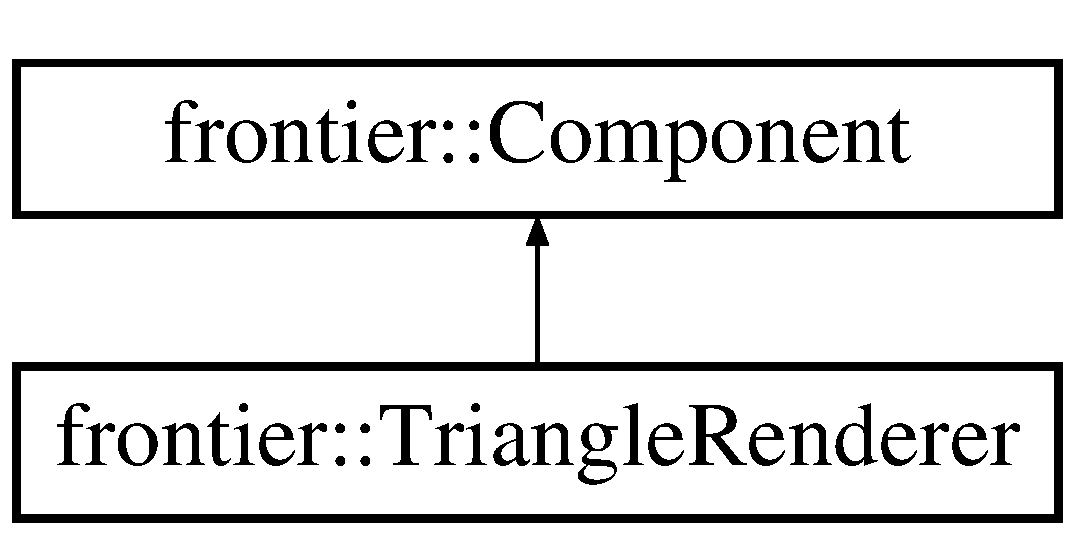
\includegraphics[height=2.000000cm]{classfrontier_1_1_triangle_renderer}
\end{center}
\end{figure}
\subsection*{Public Member Functions}
\begin{DoxyCompactItemize}
\item 
\hyperlink{classfrontier_1_1_triangle_renderer_a6ee0c85620ddc77a1c4275a00f9c28cf}{Triangle\+Renderer} ()
\item 
\hyperlink{classfrontier_1_1_triangle_renderer_a3916e1bbdb4bdfe4b4d6c93f7042a552}{$\sim$\+Triangle\+Renderer} ()
\item 
void \hyperlink{classfrontier_1_1_triangle_renderer_af67946b8641608198ae92548b7c002b5}{On\+Init} (std\+::weak\+\_\+ptr$<$ \hyperlink{classfrontier_1_1_entity}{Entity} $>$ \+\_\+parent) override
\item 
void \hyperlink{classfrontier_1_1_triangle_renderer_a1db716057c1fcc2c10500958a732963b}{On\+Tick} () override
\item 
void \hyperlink{classfrontier_1_1_triangle_renderer_a2c899b9897b149dd1c7d351c11b53272}{On\+Display} () override
\item 
void \hyperlink{classfrontier_1_1_triangle_renderer_abcfffb9fa9881768899ff231be4f936f}{Attach\+Shader\+Program} (std\+::shared\+\_\+ptr$<$ \hyperlink{classfrontier_1_1_shader}{Shader} $>$ \+\_\+new\+Shader\+Program)
\item 
std\+::shared\+\_\+ptr$<$ \hyperlink{classfrontier_1_1_shader}{Shader} $>$ \hyperlink{classfrontier_1_1_triangle_renderer_a3645cd255e151c90480903d8c5907aac}{get\+Shader\+Program} ()
\item 
void \hyperlink{classfrontier_1_1_triangle_renderer_ab8cee7fc9eb0fcb70f40a646424aff96}{Attach\+Texture} (std\+::shared\+\_\+ptr$<$ \hyperlink{classfrontier_1_1_texture}{Texture} $>$ \+\_\+new\+Texture)
\item 
std\+::shared\+\_\+ptr$<$ \hyperlink{classfrontier_1_1_texture}{Texture} $>$ \hyperlink{classfrontier_1_1_triangle_renderer_adafa2024a2d486d2abf15dda2d202344}{get\+Texture} ()
\end{DoxyCompactItemize}
\subsection*{Additional Inherited Members}


\subsection{Constructor \& Destructor Documentation}
\mbox{\Hypertarget{classfrontier_1_1_triangle_renderer_a6ee0c85620ddc77a1c4275a00f9c28cf}\label{classfrontier_1_1_triangle_renderer_a6ee0c85620ddc77a1c4275a00f9c28cf}} 
\index{frontier\+::\+Triangle\+Renderer@{frontier\+::\+Triangle\+Renderer}!Triangle\+Renderer@{Triangle\+Renderer}}
\index{Triangle\+Renderer@{Triangle\+Renderer}!frontier\+::\+Triangle\+Renderer@{frontier\+::\+Triangle\+Renderer}}
\subsubsection{\texorpdfstring{Triangle\+Renderer()}{TriangleRenderer()}}
{\footnotesize\ttfamily frontier\+::\+Triangle\+Renderer\+::\+Triangle\+Renderer (\begin{DoxyParamCaption}{ }\end{DoxyParamCaption})}

\mbox{\Hypertarget{classfrontier_1_1_triangle_renderer_a3916e1bbdb4bdfe4b4d6c93f7042a552}\label{classfrontier_1_1_triangle_renderer_a3916e1bbdb4bdfe4b4d6c93f7042a552}} 
\index{frontier\+::\+Triangle\+Renderer@{frontier\+::\+Triangle\+Renderer}!````~Triangle\+Renderer@{$\sim$\+Triangle\+Renderer}}
\index{````~Triangle\+Renderer@{$\sim$\+Triangle\+Renderer}!frontier\+::\+Triangle\+Renderer@{frontier\+::\+Triangle\+Renderer}}
\subsubsection{\texorpdfstring{$\sim$\+Triangle\+Renderer()}{~TriangleRenderer()}}
{\footnotesize\ttfamily frontier\+::\+Triangle\+Renderer\+::$\sim$\+Triangle\+Renderer (\begin{DoxyParamCaption}{ }\end{DoxyParamCaption})}



\subsection{Member Function Documentation}
\mbox{\Hypertarget{classfrontier_1_1_triangle_renderer_abcfffb9fa9881768899ff231be4f936f}\label{classfrontier_1_1_triangle_renderer_abcfffb9fa9881768899ff231be4f936f}} 
\index{frontier\+::\+Triangle\+Renderer@{frontier\+::\+Triangle\+Renderer}!Attach\+Shader\+Program@{Attach\+Shader\+Program}}
\index{Attach\+Shader\+Program@{Attach\+Shader\+Program}!frontier\+::\+Triangle\+Renderer@{frontier\+::\+Triangle\+Renderer}}
\subsubsection{\texorpdfstring{Attach\+Shader\+Program()}{AttachShaderProgram()}}
{\footnotesize\ttfamily void frontier\+::\+Triangle\+Renderer\+::\+Attach\+Shader\+Program (\begin{DoxyParamCaption}\item[{std\+::shared\+\_\+ptr$<$ \hyperlink{classfrontier_1_1_shader}{Shader} $>$}]{\+\_\+new\+Shader\+Program }\end{DoxyParamCaption})}

\mbox{\Hypertarget{classfrontier_1_1_triangle_renderer_ab8cee7fc9eb0fcb70f40a646424aff96}\label{classfrontier_1_1_triangle_renderer_ab8cee7fc9eb0fcb70f40a646424aff96}} 
\index{frontier\+::\+Triangle\+Renderer@{frontier\+::\+Triangle\+Renderer}!Attach\+Texture@{Attach\+Texture}}
\index{Attach\+Texture@{Attach\+Texture}!frontier\+::\+Triangle\+Renderer@{frontier\+::\+Triangle\+Renderer}}
\subsubsection{\texorpdfstring{Attach\+Texture()}{AttachTexture()}}
{\footnotesize\ttfamily void frontier\+::\+Triangle\+Renderer\+::\+Attach\+Texture (\begin{DoxyParamCaption}\item[{std\+::shared\+\_\+ptr$<$ \hyperlink{classfrontier_1_1_texture}{Texture} $>$}]{\+\_\+new\+Texture }\end{DoxyParamCaption})}

\mbox{\Hypertarget{classfrontier_1_1_triangle_renderer_a3645cd255e151c90480903d8c5907aac}\label{classfrontier_1_1_triangle_renderer_a3645cd255e151c90480903d8c5907aac}} 
\index{frontier\+::\+Triangle\+Renderer@{frontier\+::\+Triangle\+Renderer}!get\+Shader\+Program@{get\+Shader\+Program}}
\index{get\+Shader\+Program@{get\+Shader\+Program}!frontier\+::\+Triangle\+Renderer@{frontier\+::\+Triangle\+Renderer}}
\subsubsection{\texorpdfstring{get\+Shader\+Program()}{getShaderProgram()}}
{\footnotesize\ttfamily std\+::shared\+\_\+ptr$<$ \hyperlink{classfrontier_1_1_shader}{Shader} $>$ frontier\+::\+Triangle\+Renderer\+::get\+Shader\+Program (\begin{DoxyParamCaption}{ }\end{DoxyParamCaption})}

\mbox{\Hypertarget{classfrontier_1_1_triangle_renderer_adafa2024a2d486d2abf15dda2d202344}\label{classfrontier_1_1_triangle_renderer_adafa2024a2d486d2abf15dda2d202344}} 
\index{frontier\+::\+Triangle\+Renderer@{frontier\+::\+Triangle\+Renderer}!get\+Texture@{get\+Texture}}
\index{get\+Texture@{get\+Texture}!frontier\+::\+Triangle\+Renderer@{frontier\+::\+Triangle\+Renderer}}
\subsubsection{\texorpdfstring{get\+Texture()}{getTexture()}}
{\footnotesize\ttfamily std\+::shared\+\_\+ptr$<$ \hyperlink{classfrontier_1_1_texture}{Texture} $>$ frontier\+::\+Triangle\+Renderer\+::get\+Texture (\begin{DoxyParamCaption}{ }\end{DoxyParamCaption})}

\mbox{\Hypertarget{classfrontier_1_1_triangle_renderer_a2c899b9897b149dd1c7d351c11b53272}\label{classfrontier_1_1_triangle_renderer_a2c899b9897b149dd1c7d351c11b53272}} 
\index{frontier\+::\+Triangle\+Renderer@{frontier\+::\+Triangle\+Renderer}!On\+Display@{On\+Display}}
\index{On\+Display@{On\+Display}!frontier\+::\+Triangle\+Renderer@{frontier\+::\+Triangle\+Renderer}}
\subsubsection{\texorpdfstring{On\+Display()}{OnDisplay()}}
{\footnotesize\ttfamily void frontier\+::\+Triangle\+Renderer\+::\+On\+Display (\begin{DoxyParamCaption}{ }\end{DoxyParamCaption})\hspace{0.3cm}{\ttfamily [override]}, {\ttfamily [virtual]}}



Reimplemented from \hyperlink{classfrontier_1_1_component_a8faf337be5ba5fa3ca65c4be79d904c4}{frontier\+::\+Component}.

\mbox{\Hypertarget{classfrontier_1_1_triangle_renderer_af67946b8641608198ae92548b7c002b5}\label{classfrontier_1_1_triangle_renderer_af67946b8641608198ae92548b7c002b5}} 
\index{frontier\+::\+Triangle\+Renderer@{frontier\+::\+Triangle\+Renderer}!On\+Init@{On\+Init}}
\index{On\+Init@{On\+Init}!frontier\+::\+Triangle\+Renderer@{frontier\+::\+Triangle\+Renderer}}
\subsubsection{\texorpdfstring{On\+Init()}{OnInit()}}
{\footnotesize\ttfamily void frontier\+::\+Triangle\+Renderer\+::\+On\+Init (\begin{DoxyParamCaption}\item[{std\+::weak\+\_\+ptr$<$ \hyperlink{classfrontier_1_1_entity}{Entity} $>$}]{\+\_\+parent }\end{DoxyParamCaption})\hspace{0.3cm}{\ttfamily [override]}, {\ttfamily [virtual]}}



Reimplemented from \hyperlink{classfrontier_1_1_component_af3da02905c4d79219d9b12f260a35ad1}{frontier\+::\+Component}.

\mbox{\Hypertarget{classfrontier_1_1_triangle_renderer_a1db716057c1fcc2c10500958a732963b}\label{classfrontier_1_1_triangle_renderer_a1db716057c1fcc2c10500958a732963b}} 
\index{frontier\+::\+Triangle\+Renderer@{frontier\+::\+Triangle\+Renderer}!On\+Tick@{On\+Tick}}
\index{On\+Tick@{On\+Tick}!frontier\+::\+Triangle\+Renderer@{frontier\+::\+Triangle\+Renderer}}
\subsubsection{\texorpdfstring{On\+Tick()}{OnTick()}}
{\footnotesize\ttfamily void frontier\+::\+Triangle\+Renderer\+::\+On\+Tick (\begin{DoxyParamCaption}{ }\end{DoxyParamCaption})\hspace{0.3cm}{\ttfamily [override]}, {\ttfamily [virtual]}}



Reimplemented from \hyperlink{classfrontier_1_1_component_ab920f9bc07ce051ebb5559c5a66508d1}{frontier\+::\+Component}.



The documentation for this class was generated from the following files\+:\begin{DoxyCompactItemize}
\item 
src/myengine/\hyperlink{_triangle_renderer_8h}{Triangle\+Renderer.\+h}\item 
src/myengine/\hyperlink{_triangle_renderer_8cpp}{Triangle\+Renderer.\+cpp}\end{DoxyCompactItemize}

\hypertarget{classfrontier_1_1_u_i_button}{}\section{frontier\+:\+:U\+I\+Button Class Reference}
\label{classfrontier_1_1_u_i_button}\index{frontier\+::\+U\+I\+Button@{frontier\+::\+U\+I\+Button}}


A UI button that will be in screen space.  




{\ttfamily \#include $<$U\+I\+Button.\+h$>$}

Inheritance diagram for frontier\+:\+:U\+I\+Button\+:\begin{figure}[H]
\begin{center}
\leavevmode
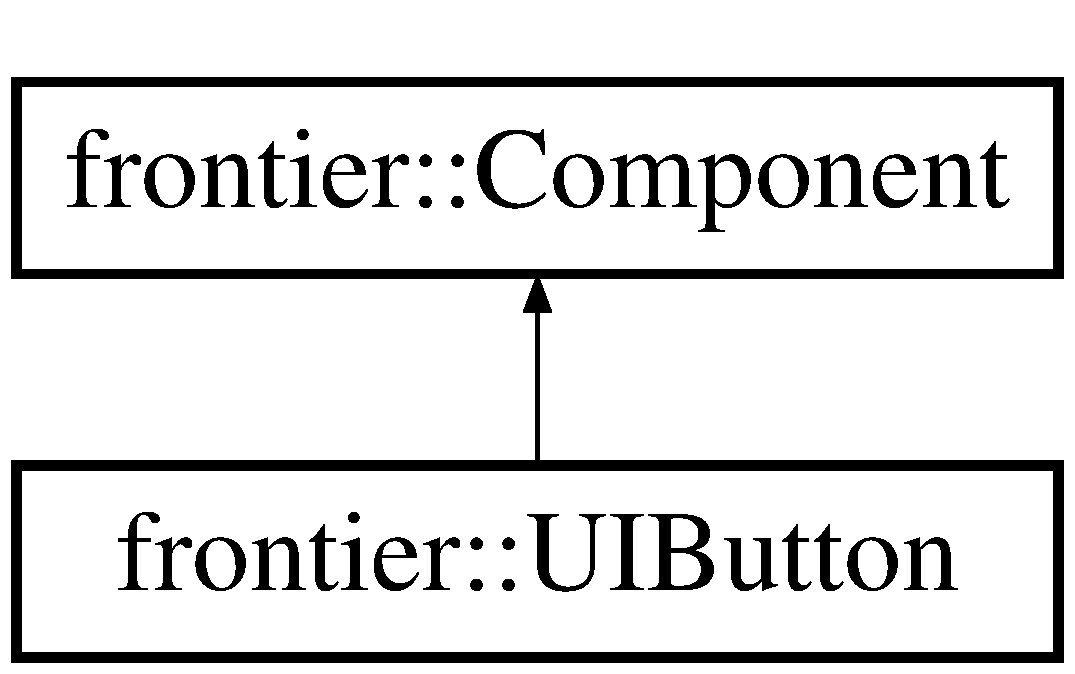
\includegraphics[height=2.000000cm]{classfrontier_1_1_u_i_button}
\end{center}
\end{figure}
\subsection*{Public Member Functions}
\begin{DoxyCompactItemize}
\item 
void \hyperlink{classfrontier_1_1_u_i_button_a1c4555865094fdd2dd9dd595740c05b0}{On\+Init} (std\+::weak\+\_\+ptr$<$ \hyperlink{classfrontier_1_1_entity}{Entity} $>$ \+\_\+parent)
\begin{DoxyCompactList}\small\item\em Initialises the UI button. \end{DoxyCompactList}\item 
void \hyperlink{classfrontier_1_1_u_i_button_a7b952033156122471f3fd6688961505f}{On\+Init} (std\+::weak\+\_\+ptr$<$ \hyperlink{classfrontier_1_1_entity}{Entity} $>$ \+\_\+parent, std\+::weak\+\_\+ptr$<$ \hyperlink{classfrontier_1_1_u_i_image}{U\+I\+Image} $>$ \+\_\+target\+Img)
\begin{DoxyCompactList}\small\item\em Initialises the UI button with a \hyperlink{classfrontier_1_1_u_i_image}{U\+I\+Image} as a target. \end{DoxyCompactList}\item 
void \hyperlink{classfrontier_1_1_u_i_button_a8eda4323e4d0c2cd2c6a4639f39a1a09}{On\+Tick} () override
\begin{DoxyCompactList}\small\item\em Updates the Button. \end{DoxyCompactList}\item 
void \hyperlink{classfrontier_1_1_u_i_button_acb2814a6d4a6303ad8606f7ae01e3f3d}{Set\+Target\+Image} (std\+::weak\+\_\+ptr$<$ \hyperlink{classfrontier_1_1_u_i_image}{U\+I\+Image} $>$ \+\_\+new\+Image)
\begin{DoxyCompactList}\small\item\em Sets a new target image. \end{DoxyCompactList}\item 
void \hyperlink{classfrontier_1_1_u_i_button_a0eade093232bc80046e2d9df0157e353}{Set\+Idle\+Color} (glm\+::vec3 \+\_\+new\+Idle\+Color)
\begin{DoxyCompactList}\small\item\em Sets a new idle color for the button. \end{DoxyCompactList}\item 
void \hyperlink{classfrontier_1_1_u_i_button_a40ac28d611b1b30112bd8bff47ade5de}{Set\+Pressed\+Color} (glm\+::vec3 \+\_\+new\+Pressed\+Color)
\begin{DoxyCompactList}\small\item\em Sets a new pressed color for the button. \end{DoxyCompactList}\item 
void \hyperlink{classfrontier_1_1_u_i_button_a3a71b90b88606a1eacb79fcb38eba42b}{Set\+Overlap\+Color} (glm\+::vec3 \+\_\+new\+Overlap\+Color)
\begin{DoxyCompactList}\small\item\em Sets a new overlap color for the button. \end{DoxyCompactList}\end{DoxyCompactItemize}
\subsection*{Additional Inherited Members}


\subsection{Detailed Description}
A UI button that will be in screen space. 

\subsection{Member Function Documentation}
\mbox{\Hypertarget{classfrontier_1_1_u_i_button_a1c4555865094fdd2dd9dd595740c05b0}\label{classfrontier_1_1_u_i_button_a1c4555865094fdd2dd9dd595740c05b0}} 
\index{frontier\+::\+U\+I\+Button@{frontier\+::\+U\+I\+Button}!On\+Init@{On\+Init}}
\index{On\+Init@{On\+Init}!frontier\+::\+U\+I\+Button@{frontier\+::\+U\+I\+Button}}
\subsubsection{\texorpdfstring{On\+Init()}{OnInit()}\hspace{0.1cm}{\footnotesize\ttfamily [1/2]}}
{\footnotesize\ttfamily void frontier\+::\+U\+I\+Button\+::\+On\+Init (\begin{DoxyParamCaption}\item[{std\+::weak\+\_\+ptr$<$ \hyperlink{classfrontier_1_1_entity}{Entity} $>$}]{\+\_\+parent }\end{DoxyParamCaption})\hspace{0.3cm}{\ttfamily [virtual]}}



Initialises the UI button. 


\begin{DoxyParams}{Parameters}
{\em \+\_\+parent} & The parent to this component. \\
\hline
\end{DoxyParams}


Reimplemented from \hyperlink{classfrontier_1_1_component_af3da02905c4d79219d9b12f260a35ad1}{frontier\+::\+Component}.

\mbox{\Hypertarget{classfrontier_1_1_u_i_button_a7b952033156122471f3fd6688961505f}\label{classfrontier_1_1_u_i_button_a7b952033156122471f3fd6688961505f}} 
\index{frontier\+::\+U\+I\+Button@{frontier\+::\+U\+I\+Button}!On\+Init@{On\+Init}}
\index{On\+Init@{On\+Init}!frontier\+::\+U\+I\+Button@{frontier\+::\+U\+I\+Button}}
\subsubsection{\texorpdfstring{On\+Init()}{OnInit()}\hspace{0.1cm}{\footnotesize\ttfamily [2/2]}}
{\footnotesize\ttfamily void frontier\+::\+U\+I\+Button\+::\+On\+Init (\begin{DoxyParamCaption}\item[{std\+::weak\+\_\+ptr$<$ \hyperlink{classfrontier_1_1_entity}{Entity} $>$}]{\+\_\+parent,  }\item[{std\+::weak\+\_\+ptr$<$ \hyperlink{classfrontier_1_1_u_i_image}{U\+I\+Image} $>$}]{\+\_\+target\+Img }\end{DoxyParamCaption})}



Initialises the UI button with a \hyperlink{classfrontier_1_1_u_i_image}{U\+I\+Image} as a target. 


\begin{DoxyParams}{Parameters}
{\em \+\_\+parent} & The parent to this component. \\
\hline
{\em \+\_\+target\+Img} & The target image for the button. \\
\hline
\end{DoxyParams}
\mbox{\Hypertarget{classfrontier_1_1_u_i_button_a8eda4323e4d0c2cd2c6a4639f39a1a09}\label{classfrontier_1_1_u_i_button_a8eda4323e4d0c2cd2c6a4639f39a1a09}} 
\index{frontier\+::\+U\+I\+Button@{frontier\+::\+U\+I\+Button}!On\+Tick@{On\+Tick}}
\index{On\+Tick@{On\+Tick}!frontier\+::\+U\+I\+Button@{frontier\+::\+U\+I\+Button}}
\subsubsection{\texorpdfstring{On\+Tick()}{OnTick()}}
{\footnotesize\ttfamily void frontier\+::\+U\+I\+Button\+::\+On\+Tick (\begin{DoxyParamCaption}{ }\end{DoxyParamCaption})\hspace{0.3cm}{\ttfamily [override]}, {\ttfamily [virtual]}}



Updates the Button. 



Reimplemented from \hyperlink{classfrontier_1_1_component_ab920f9bc07ce051ebb5559c5a66508d1}{frontier\+::\+Component}.

\mbox{\Hypertarget{classfrontier_1_1_u_i_button_a0eade093232bc80046e2d9df0157e353}\label{classfrontier_1_1_u_i_button_a0eade093232bc80046e2d9df0157e353}} 
\index{frontier\+::\+U\+I\+Button@{frontier\+::\+U\+I\+Button}!Set\+Idle\+Color@{Set\+Idle\+Color}}
\index{Set\+Idle\+Color@{Set\+Idle\+Color}!frontier\+::\+U\+I\+Button@{frontier\+::\+U\+I\+Button}}
\subsubsection{\texorpdfstring{Set\+Idle\+Color()}{SetIdleColor()}}
{\footnotesize\ttfamily void frontier\+::\+U\+I\+Button\+::\+Set\+Idle\+Color (\begin{DoxyParamCaption}\item[{glm\+::vec3}]{\+\_\+new\+Idle\+Color }\end{DoxyParamCaption})}



Sets a new idle color for the button. 

\mbox{\Hypertarget{classfrontier_1_1_u_i_button_a3a71b90b88606a1eacb79fcb38eba42b}\label{classfrontier_1_1_u_i_button_a3a71b90b88606a1eacb79fcb38eba42b}} 
\index{frontier\+::\+U\+I\+Button@{frontier\+::\+U\+I\+Button}!Set\+Overlap\+Color@{Set\+Overlap\+Color}}
\index{Set\+Overlap\+Color@{Set\+Overlap\+Color}!frontier\+::\+U\+I\+Button@{frontier\+::\+U\+I\+Button}}
\subsubsection{\texorpdfstring{Set\+Overlap\+Color()}{SetOverlapColor()}}
{\footnotesize\ttfamily void frontier\+::\+U\+I\+Button\+::\+Set\+Overlap\+Color (\begin{DoxyParamCaption}\item[{glm\+::vec3}]{\+\_\+new\+Overlap\+Color }\end{DoxyParamCaption})}



Sets a new overlap color for the button. 

\mbox{\Hypertarget{classfrontier_1_1_u_i_button_a40ac28d611b1b30112bd8bff47ade5de}\label{classfrontier_1_1_u_i_button_a40ac28d611b1b30112bd8bff47ade5de}} 
\index{frontier\+::\+U\+I\+Button@{frontier\+::\+U\+I\+Button}!Set\+Pressed\+Color@{Set\+Pressed\+Color}}
\index{Set\+Pressed\+Color@{Set\+Pressed\+Color}!frontier\+::\+U\+I\+Button@{frontier\+::\+U\+I\+Button}}
\subsubsection{\texorpdfstring{Set\+Pressed\+Color()}{SetPressedColor()}}
{\footnotesize\ttfamily void frontier\+::\+U\+I\+Button\+::\+Set\+Pressed\+Color (\begin{DoxyParamCaption}\item[{glm\+::vec3}]{\+\_\+new\+Pressed\+Color }\end{DoxyParamCaption})}



Sets a new pressed color for the button. 

\mbox{\Hypertarget{classfrontier_1_1_u_i_button_acb2814a6d4a6303ad8606f7ae01e3f3d}\label{classfrontier_1_1_u_i_button_acb2814a6d4a6303ad8606f7ae01e3f3d}} 
\index{frontier\+::\+U\+I\+Button@{frontier\+::\+U\+I\+Button}!Set\+Target\+Image@{Set\+Target\+Image}}
\index{Set\+Target\+Image@{Set\+Target\+Image}!frontier\+::\+U\+I\+Button@{frontier\+::\+U\+I\+Button}}
\subsubsection{\texorpdfstring{Set\+Target\+Image()}{SetTargetImage()}}
{\footnotesize\ttfamily void frontier\+::\+U\+I\+Button\+::\+Set\+Target\+Image (\begin{DoxyParamCaption}\item[{std\+::weak\+\_\+ptr$<$ \hyperlink{classfrontier_1_1_u_i_image}{U\+I\+Image} $>$}]{\+\_\+new\+Image }\end{DoxyParamCaption})}



Sets a new target image. 


\begin{DoxyParams}{Parameters}
{\em \+\_\+target\+Img} & The new target image for the button. \\
\hline
\end{DoxyParams}


The documentation for this class was generated from the following files\+:\begin{DoxyCompactItemize}
\item 
src/myengine/\hyperlink{_u_i_button_8h}{U\+I\+Button.\+h}\item 
src/myengine/\hyperlink{_u_i_button_8cpp}{U\+I\+Button.\+cpp}\end{DoxyCompactItemize}

\hypertarget{classfrontier_1_1_u_i_image}{}\section{frontier\+:\+:U\+I\+Image Class Reference}
\label{classfrontier_1_1_u_i_image}\index{frontier\+::\+U\+I\+Image@{frontier\+::\+U\+I\+Image}}


{\ttfamily \#include $<$U\+I\+Image.\+h$>$}

Inheritance diagram for frontier\+:\+:U\+I\+Image\+:\begin{figure}[H]
\begin{center}
\leavevmode
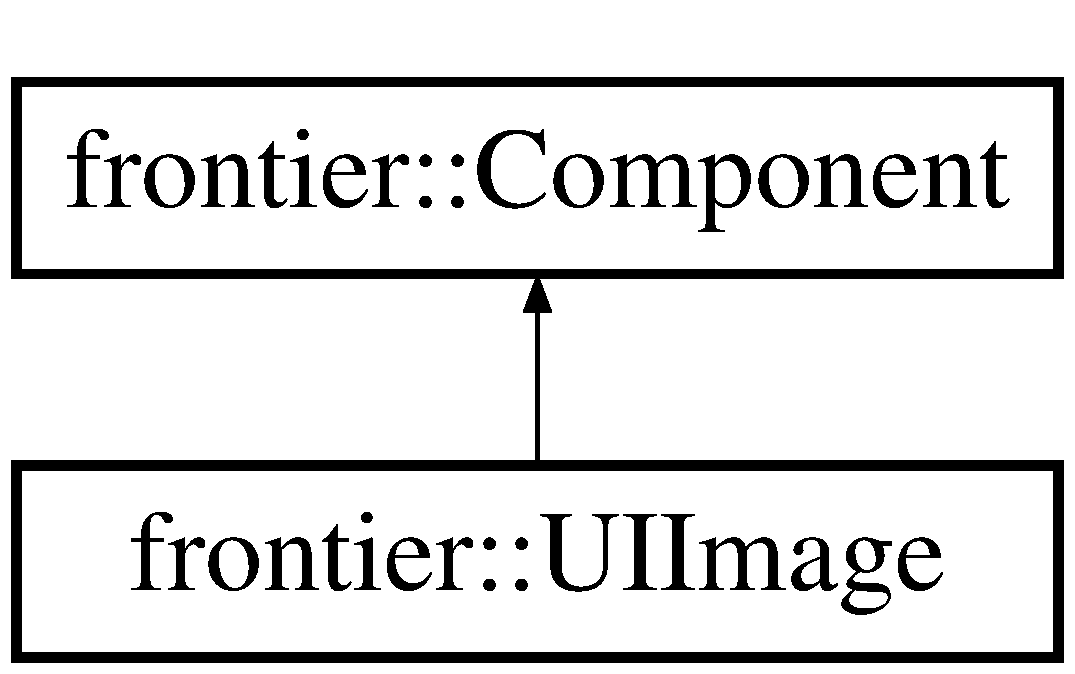
\includegraphics[height=2.000000cm]{classfrontier_1_1_u_i_image}
\end{center}
\end{figure}
\subsection*{Public Member Functions}
\begin{DoxyCompactItemize}
\item 
void \hyperlink{classfrontier_1_1_u_i_image_ad862e7dd5bcd1c2847001f5e1b56c114}{On\+Init} (std\+::weak\+\_\+ptr$<$ \hyperlink{classfrontier_1_1_entity}{Entity} $>$ \+\_\+parent)
\item 
void \hyperlink{classfrontier_1_1_u_i_image_a77205b7ee247e0ee36523e07816e10fb}{On\+Init} (std\+::weak\+\_\+ptr$<$ \hyperlink{classfrontier_1_1_entity}{Entity} $>$ \+\_\+parent, std\+::shared\+\_\+ptr$<$ \hyperlink{classfrontier_1_1_texture}{Texture} $>$ \+\_\+newtexture, bool preserve\+Aspect=false)
\item 
void \hyperlink{classfrontier_1_1_u_i_image_a4e0d055c0add55fa5e63ae892ea59498}{On\+Tick} () override
\item 
void \hyperlink{classfrontier_1_1_u_i_image_a6e734a2bc1ab3869dbed9ad0161db03e}{Attach\+Shader} (std\+::shared\+\_\+ptr$<$ \hyperlink{classfrontier_1_1_shader}{Shader} $>$ \+\_\+new\+Shader)
\item 
void \hyperlink{classfrontier_1_1_u_i_image_a879dd9d55976fb926273c4f426ab84c7}{Attach\+Texture} (std\+::shared\+\_\+ptr$<$ \hyperlink{classfrontier_1_1_texture}{Texture} $>$ \+\_\+new\+Texture, bool preserve\+Aspect=false)
\item 
void \hyperlink{classfrontier_1_1_u_i_image_ab5b455c9e918f3d2c471b18603973506}{set\+Color} (glm\+::vec4 \+\_\+new\+Color)
\end{DoxyCompactItemize}
\subsection*{Additional Inherited Members}


\subsection{Member Function Documentation}
\mbox{\Hypertarget{classfrontier_1_1_u_i_image_a6e734a2bc1ab3869dbed9ad0161db03e}\label{classfrontier_1_1_u_i_image_a6e734a2bc1ab3869dbed9ad0161db03e}} 
\index{frontier\+::\+U\+I\+Image@{frontier\+::\+U\+I\+Image}!Attach\+Shader@{Attach\+Shader}}
\index{Attach\+Shader@{Attach\+Shader}!frontier\+::\+U\+I\+Image@{frontier\+::\+U\+I\+Image}}
\subsubsection{\texorpdfstring{Attach\+Shader()}{AttachShader()}}
{\footnotesize\ttfamily void frontier\+::\+U\+I\+Image\+::\+Attach\+Shader (\begin{DoxyParamCaption}\item[{std\+::shared\+\_\+ptr$<$ \hyperlink{classfrontier_1_1_shader}{Shader} $>$}]{\+\_\+new\+Shader }\end{DoxyParamCaption})}

\mbox{\Hypertarget{classfrontier_1_1_u_i_image_a879dd9d55976fb926273c4f426ab84c7}\label{classfrontier_1_1_u_i_image_a879dd9d55976fb926273c4f426ab84c7}} 
\index{frontier\+::\+U\+I\+Image@{frontier\+::\+U\+I\+Image}!Attach\+Texture@{Attach\+Texture}}
\index{Attach\+Texture@{Attach\+Texture}!frontier\+::\+U\+I\+Image@{frontier\+::\+U\+I\+Image}}
\subsubsection{\texorpdfstring{Attach\+Texture()}{AttachTexture()}}
{\footnotesize\ttfamily void frontier\+::\+U\+I\+Image\+::\+Attach\+Texture (\begin{DoxyParamCaption}\item[{std\+::shared\+\_\+ptr$<$ \hyperlink{classfrontier_1_1_texture}{Texture} $>$}]{\+\_\+new\+Texture,  }\item[{bool}]{preserve\+Aspect = {\ttfamily false} }\end{DoxyParamCaption})}

\mbox{\Hypertarget{classfrontier_1_1_u_i_image_ad862e7dd5bcd1c2847001f5e1b56c114}\label{classfrontier_1_1_u_i_image_ad862e7dd5bcd1c2847001f5e1b56c114}} 
\index{frontier\+::\+U\+I\+Image@{frontier\+::\+U\+I\+Image}!On\+Init@{On\+Init}}
\index{On\+Init@{On\+Init}!frontier\+::\+U\+I\+Image@{frontier\+::\+U\+I\+Image}}
\subsubsection{\texorpdfstring{On\+Init()}{OnInit()}\hspace{0.1cm}{\footnotesize\ttfamily [1/2]}}
{\footnotesize\ttfamily void frontier\+::\+U\+I\+Image\+::\+On\+Init (\begin{DoxyParamCaption}\item[{std\+::weak\+\_\+ptr$<$ \hyperlink{classfrontier_1_1_entity}{Entity} $>$}]{\+\_\+parent }\end{DoxyParamCaption})\hspace{0.3cm}{\ttfamily [virtual]}}



Reimplemented from \hyperlink{classfrontier_1_1_component_af3da02905c4d79219d9b12f260a35ad1}{frontier\+::\+Component}.

\mbox{\Hypertarget{classfrontier_1_1_u_i_image_a77205b7ee247e0ee36523e07816e10fb}\label{classfrontier_1_1_u_i_image_a77205b7ee247e0ee36523e07816e10fb}} 
\index{frontier\+::\+U\+I\+Image@{frontier\+::\+U\+I\+Image}!On\+Init@{On\+Init}}
\index{On\+Init@{On\+Init}!frontier\+::\+U\+I\+Image@{frontier\+::\+U\+I\+Image}}
\subsubsection{\texorpdfstring{On\+Init()}{OnInit()}\hspace{0.1cm}{\footnotesize\ttfamily [2/2]}}
{\footnotesize\ttfamily void frontier\+::\+U\+I\+Image\+::\+On\+Init (\begin{DoxyParamCaption}\item[{std\+::weak\+\_\+ptr$<$ \hyperlink{classfrontier_1_1_entity}{Entity} $>$}]{\+\_\+parent,  }\item[{std\+::shared\+\_\+ptr$<$ \hyperlink{classfrontier_1_1_texture}{Texture} $>$}]{\+\_\+newtexture,  }\item[{bool}]{preserve\+Aspect = {\ttfamily false} }\end{DoxyParamCaption})}

\mbox{\Hypertarget{classfrontier_1_1_u_i_image_a4e0d055c0add55fa5e63ae892ea59498}\label{classfrontier_1_1_u_i_image_a4e0d055c0add55fa5e63ae892ea59498}} 
\index{frontier\+::\+U\+I\+Image@{frontier\+::\+U\+I\+Image}!On\+Tick@{On\+Tick}}
\index{On\+Tick@{On\+Tick}!frontier\+::\+U\+I\+Image@{frontier\+::\+U\+I\+Image}}
\subsubsection{\texorpdfstring{On\+Tick()}{OnTick()}}
{\footnotesize\ttfamily void frontier\+::\+U\+I\+Image\+::\+On\+Tick (\begin{DoxyParamCaption}{ }\end{DoxyParamCaption})\hspace{0.3cm}{\ttfamily [override]}, {\ttfamily [virtual]}}



Reimplemented from \hyperlink{classfrontier_1_1_component_ab920f9bc07ce051ebb5559c5a66508d1}{frontier\+::\+Component}.

\mbox{\Hypertarget{classfrontier_1_1_u_i_image_ab5b455c9e918f3d2c471b18603973506}\label{classfrontier_1_1_u_i_image_ab5b455c9e918f3d2c471b18603973506}} 
\index{frontier\+::\+U\+I\+Image@{frontier\+::\+U\+I\+Image}!set\+Color@{set\+Color}}
\index{set\+Color@{set\+Color}!frontier\+::\+U\+I\+Image@{frontier\+::\+U\+I\+Image}}
\subsubsection{\texorpdfstring{set\+Color()}{setColor()}}
{\footnotesize\ttfamily void frontier\+::\+U\+I\+Image\+::set\+Color (\begin{DoxyParamCaption}\item[{glm\+::vec4}]{\+\_\+new\+Color }\end{DoxyParamCaption})}



The documentation for this class was generated from the following files\+:\begin{DoxyCompactItemize}
\item 
src/myengine/\hyperlink{_u_i_image_8h}{U\+I\+Image.\+h}\item 
src/myengine/\hyperlink{_u_i_image_8cpp}{U\+I\+Image.\+cpp}\end{DoxyCompactItemize}

\chapter{File Documentation}
\hypertarget{_asteroid_behavior_8cpp}{}\section{src/game/\+Asteroid\+Behavior.cpp File Reference}
\label{_asteroid_behavior_8cpp}\index{src/game/\+Asteroid\+Behavior.\+cpp@{src/game/\+Asteroid\+Behavior.\+cpp}}
{\ttfamily \#include \char`\"{}Asteroid\+Behavior.\+h\char`\"{}}\newline
{\ttfamily \#include \char`\"{}myengine/\+My\+Engine.\+h\char`\"{}}\newline
{\ttfamily \#include \char`\"{}Player\+Controller.\+h\char`\"{}}\newline
{\ttfamily \#include \char`\"{}Projectile\+Behavior.\+h\char`\"{}}\newline

\hypertarget{_asteroid_behavior_8h}{}\section{src/game/\+Asteroid\+Behavior.h File Reference}
\label{_asteroid_behavior_8h}\index{src/game/\+Asteroid\+Behavior.\+h@{src/game/\+Asteroid\+Behavior.\+h}}
{\ttfamily \#include \char`\"{}glm.\+hpp\char`\"{}}\newline
{\ttfamily \#include \char`\"{}myengine/myengine.\+h\char`\"{}}\newline
\subsection*{Classes}
\begin{DoxyCompactItemize}
\item 
class \hyperlink{class_asteroid_behavior}{Asteroid\+Behavior}
\end{DoxyCompactItemize}

\hypertarget{_asteroid_spawner_8cpp}{}\section{src/game/\+Asteroid\+Spawner.cpp File Reference}
\label{_asteroid_spawner_8cpp}\index{src/game/\+Asteroid\+Spawner.\+cpp@{src/game/\+Asteroid\+Spawner.\+cpp}}
{\ttfamily \#include \char`\"{}Asteroid\+Spawner.\+h\char`\"{}}\newline
{\ttfamily \#include \char`\"{}Asteroid\+Behavior.\+h\char`\"{}}\newline
{\ttfamily \#include \char`\"{}Player\+Controller.\+h\char`\"{}}\newline

\hypertarget{_asteroid_spawner_8h}{}\section{src/game/\+Asteroid\+Spawner.h File Reference}
\label{_asteroid_spawner_8h}\index{src/game/\+Asteroid\+Spawner.\+h@{src/game/\+Asteroid\+Spawner.\+h}}
{\ttfamily \#include \char`\"{}myengine/\+My\+Engine.\+h\char`\"{}}\newline
{\ttfamily \#include \char`\"{}glm.\+hpp\char`\"{}}\newline
\subsection*{Classes}
\begin{DoxyCompactItemize}
\item 
class \hyperlink{class_asteroid_spawner}{Asteroid\+Spawner}
\end{DoxyCompactItemize}

\hypertarget{main_8cpp}{}\section{src/game/main.cpp File Reference}
\label{main_8cpp}\index{src/game/main.\+cpp@{src/game/main.\+cpp}}
{\ttfamily \#include $<$iostream$>$}\newline
{\ttfamily \#include $<$memory$>$}\newline
{\ttfamily \#include $<$myengine/\+My\+Engine.\+h$>$}\newline
{\ttfamily \#include $<$exception$>$}\newline
\subsection*{Functions}
\begin{DoxyCompactItemize}
\item 
void \hyperlink{main_8cpp_ac108aa5035d66c9a5e3c857b8e21df0b}{safe\+\_\+main} ()
\item 
int \hyperlink{main_8cpp_ae66f6b31b5ad750f1fe042a706a4e3d4}{main} ()
\end{DoxyCompactItemize}


\subsection{Function Documentation}
\mbox{\Hypertarget{main_8cpp_ae66f6b31b5ad750f1fe042a706a4e3d4}\label{main_8cpp_ae66f6b31b5ad750f1fe042a706a4e3d4}} 
\index{main.\+cpp@{main.\+cpp}!main@{main}}
\index{main@{main}!main.\+cpp@{main.\+cpp}}
\subsubsection{\texorpdfstring{main()}{main()}}
{\footnotesize\ttfamily int main (\begin{DoxyParamCaption}{ }\end{DoxyParamCaption})}

\mbox{\Hypertarget{main_8cpp_ac108aa5035d66c9a5e3c857b8e21df0b}\label{main_8cpp_ac108aa5035d66c9a5e3c857b8e21df0b}} 
\index{main.\+cpp@{main.\+cpp}!safe\+\_\+main@{safe\+\_\+main}}
\index{safe\+\_\+main@{safe\+\_\+main}!main.\+cpp@{main.\+cpp}}
\subsubsection{\texorpdfstring{safe\+\_\+main()}{safe\_main()}}
{\footnotesize\ttfamily void safe\+\_\+main (\begin{DoxyParamCaption}{ }\end{DoxyParamCaption})}


\hypertarget{_player_controller_8cpp}{}\section{src/game/\+Player\+Controller.cpp File Reference}
\label{_player_controller_8cpp}\index{src/game/\+Player\+Controller.\+cpp@{src/game/\+Player\+Controller.\+cpp}}
{\ttfamily \#include \char`\"{}Player\+Controller.\+h\char`\"{}}\newline
{\ttfamily \#include \char`\"{}myengine/\+My\+Engine.\+h\char`\"{}}\newline

\hypertarget{_player_controller_8h}{}\section{src/game/\+Player\+Controller.h File Reference}
\label{_player_controller_8h}\index{src/game/\+Player\+Controller.\+h@{src/game/\+Player\+Controller.\+h}}
{\ttfamily \#include \char`\"{}myengine/\+My\+Engine.\+h\char`\"{}}\newline
{\ttfamily \#include \char`\"{}glm.\+hpp\char`\"{}}\newline
\subsection*{Classes}
\begin{DoxyCompactItemize}
\item 
class \hyperlink{class_player_controller}{Player\+Controller}
\end{DoxyCompactItemize}

\hypertarget{_projectile_behavior_8cpp}{}\section{src/game/\+Projectile\+Behavior.cpp File Reference}
\label{_projectile_behavior_8cpp}\index{src/game/\+Projectile\+Behavior.\+cpp@{src/game/\+Projectile\+Behavior.\+cpp}}
{\ttfamily \#include \char`\"{}Projectile\+Behavior.\+h\char`\"{}}\newline
{\ttfamily \#include \char`\"{}Player\+Controller.\+h\char`\"{}}\newline

\hypertarget{_projectile_behavior_8h}{}\section{src/game/\+Projectile\+Behavior.h File Reference}
\label{_projectile_behavior_8h}\index{src/game/\+Projectile\+Behavior.\+h@{src/game/\+Projectile\+Behavior.\+h}}
{\ttfamily \#include \char`\"{}myengine/\+My\+Engine.\+h\char`\"{}}\newline
{\ttfamily \#include \char`\"{}glm.\+hpp\char`\"{}}\newline
\subsection*{Classes}
\begin{DoxyCompactItemize}
\item 
class \hyperlink{class_projectile_behavior}{Projectile\+Behavior}
\end{DoxyCompactItemize}

\hypertarget{_audio_player_8cpp}{}\section{src/myengine/\+Audio\+Player.cpp File Reference}
\label{_audio_player_8cpp}\index{src/myengine/\+Audio\+Player.\+cpp@{src/myengine/\+Audio\+Player.\+cpp}}
{\ttfamily \#include \char`\"{}Audio\+Player.\+h\char`\"{}}\newline
{\ttfamily \#include \char`\"{}Sound.\+h\char`\"{}}\newline
{\ttfamily \#include \char`\"{}Entity.\+h\char`\"{}}\newline
{\ttfamily \#include \char`\"{}Transform.\+h\char`\"{}}\newline
{\ttfamily \#include \char`\"{}Core.\+h\char`\"{}}\newline
{\ttfamily \#include \char`\"{}Camera.\+h\char`\"{}}\newline
\subsection*{Namespaces}
\begin{DoxyCompactItemize}
\item 
 \hyperlink{namespacefrontier}{frontier}
\end{DoxyCompactItemize}

\hypertarget{_audio_player_8h}{}\section{src/myengine/\+Audio\+Player.h File Reference}
\label{_audio_player_8h}\index{src/myengine/\+Audio\+Player.\+h@{src/myengine/\+Audio\+Player.\+h}}
{\ttfamily \#include \char`\"{}glm.\+hpp\char`\"{}}\newline
{\ttfamily \#include \char`\"{}Component.\+h\char`\"{}}\newline
\subsection*{Classes}
\begin{DoxyCompactItemize}
\item 
class \hyperlink{classfrontier_1_1_audio_player}{frontier\+::\+Audio\+Player}
\begin{DoxyCompactList}\small\item\em This class holds a sound resource which can then be attached to a entity can can be played in various different ways. \end{DoxyCompactList}\end{DoxyCompactItemize}
\subsection*{Namespaces}
\begin{DoxyCompactItemize}
\item 
 \hyperlink{namespacefrontier}{frontier}
\end{DoxyCompactItemize}

\hypertarget{_background_color_8cpp}{}\section{src/myengine/\+Background\+Color.cpp File Reference}
\label{_background_color_8cpp}\index{src/myengine/\+Background\+Color.\+cpp@{src/myengine/\+Background\+Color.\+cpp}}

\hypertarget{_background_color_8h}{}\section{src/myengine/\+Background\+Color.h File Reference}
\label{_background_color_8h}\index{src/myengine/\+Background\+Color.\+h@{src/myengine/\+Background\+Color.\+h}}
{\ttfamily \#include \char`\"{}glm.\+hpp\char`\"{}}\newline
{\ttfamily \#include \char`\"{}Component.\+h\char`\"{}}\newline
\subsection*{Classes}
\begin{DoxyCompactItemize}
\item 
class \hyperlink{classfrontier_1_1_back_ground_color}{frontier\+::\+Back\+Ground\+Color}
\end{DoxyCompactItemize}
\subsection*{Namespaces}
\begin{DoxyCompactItemize}
\item 
 \hyperlink{namespacefrontier}{frontier}
\end{DoxyCompactItemize}

\hypertarget{_camera_8cpp}{}\section{src/myengine/\+Camera.cpp File Reference}
\label{_camera_8cpp}\index{src/myengine/\+Camera.\+cpp@{src/myengine/\+Camera.\+cpp}}
{\ttfamily \#include \char`\"{}Camera.\+h\char`\"{}}\newline
{\ttfamily \#include \char`\"{}Core.\+h\char`\"{}}\newline
{\ttfamily \#include \char`\"{}Entity.\+h\char`\"{}}\newline
{\ttfamily \#include \char`\"{}Transform.\+h\char`\"{}}\newline
{\ttfamily \#include \char`\"{}Input.\+h\char`\"{}}\newline
{\ttfamily \#include \char`\"{}Environment.\+h\char`\"{}}\newline
{\ttfamily \#include \char`\"{}Timer.\+h\char`\"{}}\newline
{\ttfamily \#include $<$S\+D\+L2/\+S\+D\+L\+\_\+keycode.\+h$>$}\newline
{\ttfamily \#include \char`\"{}gtc/matrix\+\_\+transform.\+hpp\char`\"{}}\newline
{\ttfamily \#include \char`\"{}gtc/type\+\_\+ptr.\+hpp\char`\"{}}\newline
\subsection*{Namespaces}
\begin{DoxyCompactItemize}
\item 
 \hyperlink{namespacefrontier}{frontier}
\end{DoxyCompactItemize}

\hypertarget{_camera_8h}{}\section{src/myengine/\+Camera.h File Reference}
\label{_camera_8h}\index{src/myengine/\+Camera.\+h@{src/myengine/\+Camera.\+h}}
{\ttfamily \#include \char`\"{}glm.\+hpp\char`\"{}}\newline
{\ttfamily \#include \char`\"{}Component.\+h\char`\"{}}\newline
\subsection*{Classes}
\begin{DoxyCompactItemize}
\item 
class \hyperlink{classfrontier_1_1_camera}{frontier\+::\+Camera}
\end{DoxyCompactItemize}
\subsection*{Namespaces}
\begin{DoxyCompactItemize}
\item 
 \hyperlink{namespacefrontier}{frontier}
\end{DoxyCompactItemize}

\hypertarget{_collider_8cpp}{}\section{src/myengine/\+Collider.cpp File Reference}
\label{_collider_8cpp}\index{src/myengine/\+Collider.\+cpp@{src/myengine/\+Collider.\+cpp}}
{\ttfamily \#include \char`\"{}Collider.\+h\char`\"{}}\newline
{\ttfamily \#include \char`\"{}Core.\+h\char`\"{}}\newline
{\ttfamily \#include \char`\"{}Entity.\+h\char`\"{}}\newline
{\ttfamily \#include \char`\"{}Transform.\+h\char`\"{}}\newline
{\ttfamily \#include \char`\"{}Shader.\+h\char`\"{}}\newline
{\ttfamily \#include \char`\"{}Camera.\+h\char`\"{}}\newline
{\ttfamily \#include $<$vector$>$}\newline
{\ttfamily \#include $<$gtc/matrix\+\_\+transform.\+hpp$>$}\newline
\subsection*{Namespaces}
\begin{DoxyCompactItemize}
\item 
 \hyperlink{namespacefrontier}{frontier}
\end{DoxyCompactItemize}

\hypertarget{_collider_8h}{}\section{src/myengine/\+Collider.h File Reference}
\label{_collider_8h}\index{src/myengine/\+Collider.\+h@{src/myengine/\+Collider.\+h}}
{\ttfamily \#include \char`\"{}Component.\+h\char`\"{}}\newline
{\ttfamily \#include \char`\"{}glm.\+hpp\char`\"{}}\newline
{\ttfamily \#include $<$G\+L/glew.\+h$>$}\newline
{\ttfamily \#include $<$vector$>$}\newline
\subsection*{Classes}
\begin{DoxyCompactItemize}
\item 
class \hyperlink{classfrontier_1_1_collider}{frontier\+::\+Collider}
\end{DoxyCompactItemize}
\subsection*{Namespaces}
\begin{DoxyCompactItemize}
\item 
 \hyperlink{namespacefrontier}{frontier}
\end{DoxyCompactItemize}

\hypertarget{_component_8cpp}{}\section{src/myengine/\+Component.cpp File Reference}
\label{_component_8cpp}\index{src/myengine/\+Component.\+cpp@{src/myengine/\+Component.\+cpp}}
{\ttfamily \#include \char`\"{}Component.\+h\char`\"{}}\newline
{\ttfamily \#include \char`\"{}Entity.\+h\char`\"{}}\newline
{\ttfamily \#include \char`\"{}Core.\+h\char`\"{}}\newline
{\ttfamily \#include $<$iostream$>$}\newline
\subsection*{Namespaces}
\begin{DoxyCompactItemize}
\item 
 \hyperlink{namespacemyengine}{myengine}
\end{DoxyCompactItemize}

\hypertarget{_component_8h}{}\section{src/myengine/\+Component.h File Reference}
\label{_component_8h}\index{src/myengine/\+Component.\+h@{src/myengine/\+Component.\+h}}
{\ttfamily \#include $<$memory$>$}\newline
\subsection*{Classes}
\begin{DoxyCompactItemize}
\item 
class \hyperlink{classfrontier_1_1_component}{frontier\+::\+Component}
\end{DoxyCompactItemize}
\subsection*{Namespaces}
\begin{DoxyCompactItemize}
\item 
 \hyperlink{namespacefrontier}{frontier}
\end{DoxyCompactItemize}

\hypertarget{_core_8cpp}{}\section{src/myengine/\+Core.cpp File Reference}
\label{_core_8cpp}\index{src/myengine/\+Core.\+cpp@{src/myengine/\+Core.\+cpp}}
{\ttfamily \#include \char`\"{}Core.\+h\char`\"{}}\newline
{\ttfamily \#include \char`\"{}Entity.\+h\char`\"{}}\newline
{\ttfamily \#include \char`\"{}Environment.\+h\char`\"{}}\newline
{\ttfamily \#include \char`\"{}Resources.\+h\char`\"{}}\newline
{\ttfamily \#include \char`\"{}Camera.\+h\char`\"{}}\newline
{\ttfamily \#include \char`\"{}Input.\+h\char`\"{}}\newline
{\ttfamily \#include \char`\"{}Timer.\+h\char`\"{}}\newline
{\ttfamily \#include \char`\"{}Shader.\+h\char`\"{}}\newline
{\ttfamily \#include \char`\"{}Prefab.\+h\char`\"{}}\newline
{\ttfamily \#include \char`\"{}Pooler.\+h\char`\"{}}\newline
{\ttfamily \#include $<$iostream$>$}\newline
{\ttfamily \#include $<$G\+L/glew.\+h$>$}\newline
{\ttfamily \#include $<$map$>$}\newline
{\ttfamily \#include $<$exception$>$}\newline
\subsection*{Namespaces}
\begin{DoxyCompactItemize}
\item 
 \hyperlink{namespacefrontier}{frontier}
\end{DoxyCompactItemize}

\hypertarget{_core_8h}{}\section{src/myengine/\+Core.h File Reference}
\label{_core_8h}\index{src/myengine/\+Core.\+h@{src/myengine/\+Core.\+h}}
{\ttfamily \#include $<$memory$>$}\newline
{\ttfamily \#include $<$vector$>$}\newline
{\ttfamily \#include $<$S\+D\+L2/\+S\+D\+L.\+h$>$}\newline
{\ttfamily \#include \char`\"{}glm.\+hpp\char`\"{}}\newline
{\ttfamily \#include $<$string$>$}\newline
{\ttfamily \#include $<$A\+L/al.\+h$>$}\newline
{\ttfamily \#include $<$A\+L/alc.\+h$>$}\newline
\subsection*{Classes}
\begin{DoxyCompactItemize}
\item 
class \hyperlink{classfrontier_1_1_core}{frontier\+::\+Core}
\begin{DoxyCompactList}\small\item\em The main core of the engine. This is where all entities, prefabs and resources get created. \end{DoxyCompactList}\end{DoxyCompactItemize}
\subsection*{Namespaces}
\begin{DoxyCompactItemize}
\item 
 \hyperlink{namespacefrontier}{frontier}
\end{DoxyCompactItemize}

\hypertarget{_cubemap_texture_8cpp}{}\section{src/myengine/\+Cubemap\+Texture.cpp File Reference}
\label{_cubemap_texture_8cpp}\index{src/myengine/\+Cubemap\+Texture.\+cpp@{src/myengine/\+Cubemap\+Texture.\+cpp}}
{\ttfamily \#include $<$stb\+\_\+image.\+h$>$}\newline
{\ttfamily \#include $<$iostream$>$}\newline
{\ttfamily \#include $<$exception$>$}\newline
{\ttfamily \#include \char`\"{}Cubemap\+Texture.\+h\char`\"{}}\newline
{\ttfamily \#include \char`\"{}Resources.\+h\char`\"{}}\newline
\subsection*{Namespaces}
\begin{DoxyCompactItemize}
\item 
 \hyperlink{namespacefrontier}{frontier}
\end{DoxyCompactItemize}

\hypertarget{_cubemap_texture_8h}{}\section{src/myengine/\+Cubemap\+Texture.h File Reference}
\label{_cubemap_texture_8h}\index{src/myengine/\+Cubemap\+Texture.\+h@{src/myengine/\+Cubemap\+Texture.\+h}}
{\ttfamily \#include $<$memory$>$}\newline
{\ttfamily \#include $<$string$>$}\newline
{\ttfamily \#include $<$vector$>$}\newline
{\ttfamily \#include $<$G\+L/glew.\+h$>$}\newline
{\ttfamily \#include \char`\"{}Resource.\+h\char`\"{}}\newline
\subsection*{Classes}
\begin{DoxyCompactItemize}
\item 
class \hyperlink{classfrontier_1_1_cubemap_texture}{frontier\+::\+Cubemap\+Texture}
\begin{DoxyCompactList}\small\item\em \hyperlink{classfrontier_1_1_resource}{Resource} class for a cubemap texture, mainly used for skyboxes. \end{DoxyCompactList}\end{DoxyCompactItemize}
\subsection*{Namespaces}
\begin{DoxyCompactItemize}
\item 
 \hyperlink{namespacefrontier}{frontier}
\end{DoxyCompactItemize}

\hypertarget{_entity_8cpp}{}\section{src/myengine/\+Entity.cpp File Reference}
\label{_entity_8cpp}\index{src/myengine/\+Entity.\+cpp@{src/myengine/\+Entity.\+cpp}}
{\ttfamily \#include \char`\"{}Entity.\+h\char`\"{}}\newline
{\ttfamily \#include \char`\"{}Component.\+h\char`\"{}}\newline
{\ttfamily \#include \char`\"{}Transform.\+h\char`\"{}}\newline
{\ttfamily \#include \char`\"{}Prefab.\+h\char`\"{}}\newline
{\ttfamily \#include \char`\"{}Mesh\+Renderer.\+h\char`\"{}}\newline
{\ttfamily \#include \char`\"{}Collider.\+h\char`\"{}}\newline
{\ttfamily \#include \char`\"{}game/\+Asteroid\+Behavior.\+h\char`\"{}}\newline
{\ttfamily \#include \char`\"{}game/\+Projectile\+Behavior.\+h\char`\"{}}\newline
{\ttfamily \#include $<$iostream$>$}\newline
\subsection*{Namespaces}
\begin{DoxyCompactItemize}
\item 
 \hyperlink{namespacefrontier}{frontier}
\end{DoxyCompactItemize}

\hypertarget{_entity_8h}{}\section{src/myengine/\+Entity.h File Reference}
\label{_entity_8h}\index{src/myengine/\+Entity.\+h@{src/myengine/\+Entity.\+h}}
{\ttfamily \#include $<$vector$>$}\newline
{\ttfamily \#include $<$memory$>$}\newline
{\ttfamily \#include $<$type\+\_\+traits$>$}\newline
{\ttfamily \#include $<$typeinfo$>$}\newline
{\ttfamily \#include $<$iostream$>$}\newline
{\ttfamily \#include $<$assert.\+h$>$}\newline
{\ttfamily \#include \char`\"{}Component.\+h\char`\"{}}\newline
{\ttfamily \#include \char`\"{}glm.\+hpp\char`\"{}}\newline
\subsection*{Classes}
\begin{DoxyCompactItemize}
\item 
class \hyperlink{classfrontier_1_1_entity}{frontier\+::\+Entity}
\end{DoxyCompactItemize}
\subsection*{Namespaces}
\begin{DoxyCompactItemize}
\item 
 \hyperlink{namespacefrontier}{frontier}
\end{DoxyCompactItemize}

\hypertarget{_environment_8cpp}{}\section{src/myengine/\+Environment.cpp File Reference}
\label{_environment_8cpp}\index{src/myengine/\+Environment.\+cpp@{src/myengine/\+Environment.\+cpp}}
{\ttfamily \#include \char`\"{}Environment.\+h\char`\"{}}\newline
{\ttfamily \#include $<$iostream$>$}\newline
\subsection*{Namespaces}
\begin{DoxyCompactItemize}
\item 
 \hyperlink{namespacemyengine}{myengine}
\end{DoxyCompactItemize}

\hypertarget{_environment_8h}{}\section{src/myengine/\+Environment.h File Reference}
\label{_environment_8h}\index{src/myengine/\+Environment.\+h@{src/myengine/\+Environment.\+h}}
{\ttfamily \#include $<$S\+D\+L2/\+S\+D\+L.\+h$>$}\newline
{\ttfamily \#include $<$memory$>$}\newline
\subsection*{Classes}
\begin{DoxyCompactItemize}
\item 
class \hyperlink{classfrontier_1_1_environment}{frontier\+::\+Environment}
\end{DoxyCompactItemize}
\subsection*{Namespaces}
\begin{DoxyCompactItemize}
\item 
 \hyperlink{namespacefrontier}{frontier}
\end{DoxyCompactItemize}

\hypertarget{_input_8cpp}{}\section{src/myengine/\+Input.cpp File Reference}
\label{_input_8cpp}\index{src/myengine/\+Input.\+cpp@{src/myengine/\+Input.\+cpp}}

\hypertarget{_input_8h}{}\section{src/myengine/\+Input.h File Reference}
\label{_input_8h}\index{src/myengine/\+Input.\+h@{src/myengine/\+Input.\+h}}
{\ttfamily \#include $<$S\+D\+L2/\+S\+D\+L.\+h$>$}\newline
{\ttfamily \#include $<$S\+D\+L2/\+S\+D\+L\+\_\+keycode.\+h$>$}\newline
{\ttfamily \#include $<$memory$>$}\newline
{\ttfamily \#include $<$map$>$}\newline
{\ttfamily \#include \char`\"{}glm.\+hpp\char`\"{}}\newline
\subsection*{Classes}
\begin{DoxyCompactItemize}
\item 
class \hyperlink{classfrontier_1_1_input}{frontier\+::\+Input}
\end{DoxyCompactItemize}
\subsection*{Namespaces}
\begin{DoxyCompactItemize}
\item 
 \hyperlink{namespacefrontier}{frontier}
\end{DoxyCompactItemize}

\hypertarget{_mesh_8cpp}{}\section{src/myengine/\+Mesh.cpp File Reference}
\label{_mesh_8cpp}\index{src/myengine/\+Mesh.\+cpp@{src/myengine/\+Mesh.\+cpp}}

\hypertarget{_mesh_8h}{}\section{src/myengine/\+Mesh.h File Reference}
\label{_mesh_8h}\index{src/myengine/\+Mesh.\+h@{src/myengine/\+Mesh.\+h}}
{\ttfamily \#include \char`\"{}glm.\+hpp\char`\"{}}\newline
{\ttfamily \#include \char`\"{}Shader.\+h\char`\"{}}\newline
{\ttfamily \#include $<$string$>$}\newline
{\ttfamily \#include $<$vector$>$}\newline
{\ttfamily \#include $<$memory$>$}\newline
{\ttfamily \#include $<$G\+L/glew.\+h$>$}\newline
\subsection*{Classes}
\begin{DoxyCompactItemize}
\item 
class \hyperlink{classfrontier_1_1_mesh}{frontier\+::\+Mesh}
\begin{DoxyCompactList}\small\item\em Contains vertices, normals and texcoords loaded from an obj. \end{DoxyCompactList}\end{DoxyCompactItemize}
\subsection*{Namespaces}
\begin{DoxyCompactItemize}
\item 
 \hyperlink{namespacefrontier}{frontier}
\end{DoxyCompactItemize}

\hypertarget{_mesh_renderer_8cpp}{}\section{src/myengine/\+Mesh\+Renderer.cpp File Reference}
\label{_mesh_renderer_8cpp}\index{src/myengine/\+Mesh\+Renderer.\+cpp@{src/myengine/\+Mesh\+Renderer.\+cpp}}
{\ttfamily \#include \char`\"{}Mesh\+Renderer.\+h\char`\"{}}\newline
{\ttfamily \#include \char`\"{}Shader.\+h\char`\"{}}\newline
{\ttfamily \#include \char`\"{}Entity.\+h\char`\"{}}\newline
{\ttfamily \#include \char`\"{}Transform.\+h\char`\"{}}\newline
{\ttfamily \#include \char`\"{}Core.\+h\char`\"{}}\newline
{\ttfamily \#include \char`\"{}Camera.\+h\char`\"{}}\newline
{\ttfamily \#include \char`\"{}Texture.\+h\char`\"{}}\newline
{\ttfamily \#include \char`\"{}Model.\+h\char`\"{}}\newline
\subsection*{Namespaces}
\begin{DoxyCompactItemize}
\item 
 \hyperlink{namespacefrontier}{frontier}
\end{DoxyCompactItemize}

\hypertarget{_mesh_renderer_8h}{}\section{src/myengine/\+Mesh\+Renderer.h File Reference}
\label{_mesh_renderer_8h}\index{src/myengine/\+Mesh\+Renderer.\+h@{src/myengine/\+Mesh\+Renderer.\+h}}
{\ttfamily \#include $<$G\+L/glew.\+h$>$}\newline
{\ttfamily \#include $<$memory$>$}\newline
{\ttfamily \#include $<$vector$>$}\newline
{\ttfamily \#include \char`\"{}Component.\+h\char`\"{}}\newline
{\ttfamily \#include \char`\"{}glm.\+hpp\char`\"{}}\newline
\subsection*{Classes}
\begin{DoxyCompactItemize}
\item 
class \hyperlink{classfrontier_1_1_mesh_renderer}{frontier\+::\+Mesh\+Renderer}
\end{DoxyCompactItemize}
\subsection*{Namespaces}
\begin{DoxyCompactItemize}
\item 
 \hyperlink{namespacefrontier}{frontier}
\end{DoxyCompactItemize}

\hypertarget{_model_8cpp}{}\section{src/myengine/\+Model.cpp File Reference}
\label{_model_8cpp}\index{src/myengine/\+Model.\+cpp@{src/myengine/\+Model.\+cpp}}
{\ttfamily \#include \char`\"{}tiny\+\_\+obj\+\_\+loader.\+h\char`\"{}}\newline
{\ttfamily \#include \char`\"{}Model.\+h\char`\"{}}\newline
{\ttfamily \#include \char`\"{}Mesh.\+h\char`\"{}}\newline
{\ttfamily \#include $<$iostream$>$}\newline
\subsection*{Namespaces}
\begin{DoxyCompactItemize}
\item 
 \hyperlink{namespacefrontier}{frontier}
\end{DoxyCompactItemize}
\subsection*{Macros}
\begin{DoxyCompactItemize}
\item 
\#define \hyperlink{_model_8cpp_af14fac7fbc250522a78849d58d5b0811}{T\+I\+N\+Y\+O\+B\+J\+L\+O\+A\+D\+E\+R\+\_\+\+I\+M\+P\+L\+E\+M\+E\+N\+T\+A\+T\+I\+ON}
\end{DoxyCompactItemize}


\subsection{Macro Definition Documentation}
\mbox{\Hypertarget{_model_8cpp_af14fac7fbc250522a78849d58d5b0811}\label{_model_8cpp_af14fac7fbc250522a78849d58d5b0811}} 
\index{Model.\+cpp@{Model.\+cpp}!T\+I\+N\+Y\+O\+B\+J\+L\+O\+A\+D\+E\+R\+\_\+\+I\+M\+P\+L\+E\+M\+E\+N\+T\+A\+T\+I\+ON@{T\+I\+N\+Y\+O\+B\+J\+L\+O\+A\+D\+E\+R\+\_\+\+I\+M\+P\+L\+E\+M\+E\+N\+T\+A\+T\+I\+ON}}
\index{T\+I\+N\+Y\+O\+B\+J\+L\+O\+A\+D\+E\+R\+\_\+\+I\+M\+P\+L\+E\+M\+E\+N\+T\+A\+T\+I\+ON@{T\+I\+N\+Y\+O\+B\+J\+L\+O\+A\+D\+E\+R\+\_\+\+I\+M\+P\+L\+E\+M\+E\+N\+T\+A\+T\+I\+ON}!Model.\+cpp@{Model.\+cpp}}
\subsubsection{\texorpdfstring{T\+I\+N\+Y\+O\+B\+J\+L\+O\+A\+D\+E\+R\+\_\+\+I\+M\+P\+L\+E\+M\+E\+N\+T\+A\+T\+I\+ON}{TINYOBJLOADER\_IMPLEMENTATION}}
{\footnotesize\ttfamily \#define T\+I\+N\+Y\+O\+B\+J\+L\+O\+A\+D\+E\+R\+\_\+\+I\+M\+P\+L\+E\+M\+E\+N\+T\+A\+T\+I\+ON}


\hypertarget{_model_8h}{}\section{src/myengine/\+Model.h File Reference}
\label{_model_8h}\index{src/myengine/\+Model.\+h@{src/myengine/\+Model.\+h}}
{\ttfamily \#include \char`\"{}Shader.\+h\char`\"{}}\newline
{\ttfamily \#include \char`\"{}Component.\+h\char`\"{}}\newline
{\ttfamily \#include \char`\"{}Resource.\+h\char`\"{}}\newline
{\ttfamily \#include \char`\"{}Resources.\+h\char`\"{}}\newline
{\ttfamily \#include $<$vector$>$}\newline
{\ttfamily \#include $<$string$>$}\newline
\subsection*{Classes}
\begin{DoxyCompactItemize}
\item 
class \hyperlink{classfrontier_1_1_model}{frontier\+::\+Model}
\end{DoxyCompactItemize}
\subsection*{Namespaces}
\begin{DoxyCompactItemize}
\item 
 \hyperlink{namespacefrontier}{frontier}
\end{DoxyCompactItemize}

\hypertarget{_my_engine_8h}{}\section{src/myengine/\+My\+Engine.h File Reference}
\label{_my_engine_8h}\index{src/myengine/\+My\+Engine.\+h@{src/myengine/\+My\+Engine.\+h}}
{\ttfamily \#include \char`\"{}Component.\+h\char`\"{}}\newline
{\ttfamily \#include \char`\"{}Core.\+h\char`\"{}}\newline
{\ttfamily \#include \char`\"{}Entity.\+h\char`\"{}}\newline
{\ttfamily \#include \char`\"{}Environment.\+h\char`\"{}}\newline
{\ttfamily \#include \char`\"{}Input.\+h\char`\"{}}\newline
{\ttfamily \#include \char`\"{}Mesh.\+h\char`\"{}}\newline
{\ttfamily \#include \char`\"{}Resource.\+h\char`\"{}}\newline
{\ttfamily \#include \char`\"{}Shader.\+h\char`\"{}}\newline
{\ttfamily \#include \char`\"{}Texture.\+h\char`\"{}}\newline
{\ttfamily \#include \char`\"{}Resources.\+h\char`\"{}}\newline
{\ttfamily \#include \char`\"{}Camera.\+h\char`\"{}}\newline
{\ttfamily \#include \char`\"{}Transform.\+h\char`\"{}}\newline
{\ttfamily \#include \char`\"{}Mesh\+Renderer.\+h\char`\"{}}\newline
{\ttfamily \#include \char`\"{}Model.\+h\char`\"{}}\newline
{\ttfamily \#include \char`\"{}Sound.\+h\char`\"{}}\newline
{\ttfamily \#include \char`\"{}Audio\+Player.\+h\char`\"{}}\newline
{\ttfamily \#include \char`\"{}Skybox.\+h\char`\"{}}\newline
{\ttfamily \#include \char`\"{}Cubemap\+Texture.\+h\char`\"{}}\newline
{\ttfamily \#include \char`\"{}Collider.\+h\char`\"{}}\newline
{\ttfamily \#include \char`\"{}U\+I\+Image.\+h\char`\"{}}\newline
{\ttfamily \#include \char`\"{}U\+I\+Button.\+h\char`\"{}}\newline
{\ttfamily \#include \char`\"{}Prefab.\+h\char`\"{}}\newline
{\ttfamily \#include \char`\"{}Pooler.\+h\char`\"{}}\newline

\hypertarget{_pooler_8cpp}{}\section{src/myengine/\+Pooler.cpp File Reference}
\label{_pooler_8cpp}\index{src/myengine/\+Pooler.\+cpp@{src/myengine/\+Pooler.\+cpp}}
{\ttfamily \#include \char`\"{}Pooler.\+h\char`\"{}}\newline
{\ttfamily \#include \char`\"{}Core.\+h\char`\"{}}\newline
{\ttfamily \#include \char`\"{}Entity.\+h\char`\"{}}\newline
{\ttfamily \#include \char`\"{}Transform.\+h\char`\"{}}\newline
\subsection*{Namespaces}
\begin{DoxyCompactItemize}
\item 
 \hyperlink{namespacefrontier}{frontier}
\end{DoxyCompactItemize}

\hypertarget{_pooler_8h}{}\section{src/myengine/\+Pooler.h File Reference}
\label{_pooler_8h}\index{src/myengine/\+Pooler.\+h@{src/myengine/\+Pooler.\+h}}
{\ttfamily \#include $<$string$>$}\newline
{\ttfamily \#include $<$memory$>$}\newline
{\ttfamily \#include $<$vector$>$}\newline
{\ttfamily \#include \char`\"{}glm.\+hpp\char`\"{}}\newline
\subsection*{Classes}
\begin{DoxyCompactItemize}
\item 
class \hyperlink{classfrontier_1_1_pooler}{frontier\+::\+Pooler}
\end{DoxyCompactItemize}
\subsection*{Namespaces}
\begin{DoxyCompactItemize}
\item 
 \hyperlink{namespacefrontier}{frontier}
\end{DoxyCompactItemize}

\hypertarget{_prefab_8cpp}{}\section{src/myengine/\+Prefab.cpp File Reference}
\label{_prefab_8cpp}\index{src/myengine/\+Prefab.\+cpp@{src/myengine/\+Prefab.\+cpp}}
{\ttfamily \#include \char`\"{}Prefab.\+h\char`\"{}}\newline
\subsection*{Namespaces}
\begin{DoxyCompactItemize}
\item 
 \hyperlink{namespacefrontier}{frontier}
\end{DoxyCompactItemize}

\hypertarget{_prefab_8h}{}\section{src/myengine/\+Prefab.h File Reference}
\label{_prefab_8h}\index{src/myengine/\+Prefab.\+h@{src/myengine/\+Prefab.\+h}}
{\ttfamily \#include $<$vector$>$}\newline
{\ttfamily \#include $<$memory$>$}\newline
{\ttfamily \#include \char`\"{}Transform.\+h\char`\"{}}\newline
{\ttfamily \#include \char`\"{}Component.\+h\char`\"{}}\newline
{\ttfamily \#include \char`\"{}Entity.\+h\char`\"{}}\newline
\subsection*{Classes}
\begin{DoxyCompactItemize}
\item 
class \hyperlink{classfrontier_1_1_prefab}{frontier\+::\+Prefab}
\begin{DoxyCompactList}\small\item\em Acts as a template for an entity, can be passed into a new entity and the information stored will pass on to the new entity. \end{DoxyCompactList}\end{DoxyCompactItemize}
\subsection*{Namespaces}
\begin{DoxyCompactItemize}
\item 
 \hyperlink{namespacefrontier}{frontier}
\end{DoxyCompactItemize}

\hypertarget{_resource_8cpp}{}\section{src/myengine/\+Resource.cpp File Reference}
\label{_resource_8cpp}\index{src/myengine/\+Resource.\+cpp@{src/myengine/\+Resource.\+cpp}}
{\ttfamily \#include \char`\"{}Resource.\+h\char`\"{}}\newline
{\ttfamily \#include $<$iostream$>$}\newline
\subsection*{Namespaces}
\begin{DoxyCompactItemize}
\item 
 \hyperlink{namespacefrontier}{frontier}
\end{DoxyCompactItemize}

\hypertarget{_resource_8h}{}\section{src/myengine/\+Resource.h File Reference}
\label{_resource_8h}\index{src/myengine/\+Resource.\+h@{src/myengine/\+Resource.\+h}}
{\ttfamily \#include $<$string$>$}\newline
{\ttfamily \#include $<$memory$>$}\newline
\subsection*{Classes}
\begin{DoxyCompactItemize}
\item 
class \hyperlink{classfrontier_1_1_resource}{frontier\+::\+Resource}
\begin{DoxyCompactList}\small\item\em Base class for a resource, all other resource types derive from this. \end{DoxyCompactList}\end{DoxyCompactItemize}
\subsection*{Namespaces}
\begin{DoxyCompactItemize}
\item 
 \hyperlink{namespacefrontier}{frontier}
\end{DoxyCompactItemize}

\hypertarget{_resources_8cpp}{}\section{src/myengine/\+Resources.cpp File Reference}
\label{_resources_8cpp}\index{src/myengine/\+Resources.\+cpp@{src/myengine/\+Resources.\+cpp}}
{\ttfamily \#include \char`\"{}Resources.\+h\char`\"{}}\newline
{\ttfamily \#include $<$iostream$>$}\newline
\subsection*{Namespaces}
\begin{DoxyCompactItemize}
\item 
 \hyperlink{namespacefrontier}{frontier}
\end{DoxyCompactItemize}

\hypertarget{_resources_8h}{}\section{src/myengine/\+Resources.h File Reference}
\label{_resources_8h}\index{src/myengine/\+Resources.\+h@{src/myengine/\+Resources.\+h}}
{\ttfamily \#include $<$list$>$}\newline
{\ttfamily \#include $<$memory$>$}\newline
{\ttfamily \#include \char`\"{}Resource.\+h\char`\"{}}\newline
\subsection*{Classes}
\begin{DoxyCompactItemize}
\item 
class \hyperlink{classmyengine_1_1_resources}{myengine\+::\+Resources}
\end{DoxyCompactItemize}
\subsection*{Namespaces}
\begin{DoxyCompactItemize}
\item 
 \hyperlink{namespacemyengine}{myengine}
\end{DoxyCompactItemize}

\hypertarget{_shader_8cpp}{}\section{src/myengine/\+Shader.cpp File Reference}
\label{_shader_8cpp}\index{src/myengine/\+Shader.\+cpp@{src/myengine/\+Shader.\+cpp}}
{\ttfamily \#include \char`\"{}Shader.\+h\char`\"{}}\newline
{\ttfamily \#include \char`\"{}Resources.\+h\char`\"{}}\newline
{\ttfamily \#include \char`\"{}Texture.\+h\char`\"{}}\newline
{\ttfamily \#include $<$fstream$>$}\newline
{\ttfamily \#include $<$sstream$>$}\newline
{\ttfamily \#include $<$iostream$>$}\newline
\subsection*{Namespaces}
\begin{DoxyCompactItemize}
\item 
 \hyperlink{namespacemyengine}{myengine}
\end{DoxyCompactItemize}

\hypertarget{_shader_8h}{}\section{src/myengine/\+Shader.h File Reference}
\label{_shader_8h}\index{src/myengine/\+Shader.\+h@{src/myengine/\+Shader.\+h}}
{\ttfamily \#include \char`\"{}Resource.\+h\char`\"{}}\newline
{\ttfamily \#include \char`\"{}glm.\+hpp\char`\"{}}\newline
{\ttfamily \#include $<$G\+L/glew.\+h$>$}\newline
{\ttfamily \#include $<$memory$>$}\newline
{\ttfamily \#include $<$vector$>$}\newline
\subsection*{Classes}
\begin{DoxyCompactItemize}
\item 
class \hyperlink{classfrontier_1_1_shader}{frontier\+::\+Shader}
\end{DoxyCompactItemize}
\subsection*{Namespaces}
\begin{DoxyCompactItemize}
\item 
 \hyperlink{namespacefrontier}{frontier}
\end{DoxyCompactItemize}

\hypertarget{_skybox_8cpp}{}\section{src/myengine/\+Skybox.cpp File Reference}
\label{_skybox_8cpp}\index{src/myengine/\+Skybox.\+cpp@{src/myengine/\+Skybox.\+cpp}}
{\ttfamily \#include \char`\"{}Skybox.\+h\char`\"{}}\newline
{\ttfamily \#include \char`\"{}Shader.\+h\char`\"{}}\newline
{\ttfamily \#include \char`\"{}Entity.\+h\char`\"{}}\newline
{\ttfamily \#include \char`\"{}Core.\+h\char`\"{}}\newline
{\ttfamily \#include \char`\"{}Cubemap\+Texture.\+h\char`\"{}}\newline
{\ttfamily \#include \char`\"{}Camera.\+h\char`\"{}}\newline
{\ttfamily \#include $<$gtc/matrix\+\_\+transform.\+hpp$>$}\newline
\subsection*{Namespaces}
\begin{DoxyCompactItemize}
\item 
 \hyperlink{namespacefrontier}{frontier}
\end{DoxyCompactItemize}

\hypertarget{_skybox_8h}{}\section{src/myengine/\+Skybox.h File Reference}
\label{_skybox_8h}\index{src/myengine/\+Skybox.\+h@{src/myengine/\+Skybox.\+h}}
{\ttfamily \#include \char`\"{}Component.\+h\char`\"{}}\newline
{\ttfamily \#include $<$memory$>$}\newline
{\ttfamily \#include $<$vector$>$}\newline
{\ttfamily \#include $<$G\+L/glew.\+h$>$}\newline
\subsection*{Classes}
\begin{DoxyCompactItemize}
\item 
class \hyperlink{classfrontier_1_1_skybox}{frontier\+::\+Skybox}
\end{DoxyCompactItemize}
\subsection*{Namespaces}
\begin{DoxyCompactItemize}
\item 
 \hyperlink{namespacefrontier}{frontier}
\end{DoxyCompactItemize}

\hypertarget{_sound_8cpp}{}\section{src/myengine/\+Sound.cpp File Reference}
\label{_sound_8cpp}\index{src/myengine/\+Sound.\+cpp@{src/myengine/\+Sound.\+cpp}}
{\ttfamily \#include \char`\"{}Sound.\+h\char`\"{}}\newline
{\ttfamily \#include \char`\"{}Resources.\+h\char`\"{}}\newline
{\ttfamily \#include $<$vorbis/vorbisfile.\+h$>$}\newline
{\ttfamily \#include $<$iostream$>$}\newline
{\ttfamily \#include $<$vector$>$}\newline
\subsection*{Classes}
\begin{DoxyCompactItemize}
\item 
struct \hyperlink{structfrontier_1_1_sound_impl}{frontier\+::\+Sound\+Impl}
\end{DoxyCompactItemize}
\subsection*{Namespaces}
\begin{DoxyCompactItemize}
\item 
 \hyperlink{namespacefrontier}{frontier}
\end{DoxyCompactItemize}

\hypertarget{_sound_8h}{}\section{src/myengine/\+Sound.h File Reference}
\label{_sound_8h}\index{src/myengine/\+Sound.\+h@{src/myengine/\+Sound.\+h}}
{\ttfamily \#include $<$memory$>$}\newline
{\ttfamily \#include $<$string$>$}\newline
{\ttfamily \#include $<$A\+L/al.\+h$>$}\newline
{\ttfamily \#include \char`\"{}glm.\+hpp\char`\"{}}\newline
{\ttfamily \#include \char`\"{}Resource.\+h\char`\"{}}\newline
\subsection*{Classes}
\begin{DoxyCompactItemize}
\item 
class \hyperlink{classfrontier_1_1_sound}{frontier\+::\+Sound}
\begin{DoxyCompactList}\small\item\em Container for a sound. Uses Open\+AL. \end{DoxyCompactList}\end{DoxyCompactItemize}
\subsection*{Namespaces}
\begin{DoxyCompactItemize}
\item 
 \hyperlink{namespacefrontier}{frontier}
\end{DoxyCompactItemize}

\hypertarget{_texture_8cpp}{}\section{src/myengine/\+Texture.cpp File Reference}
\label{_texture_8cpp}\index{src/myengine/\+Texture.\+cpp@{src/myengine/\+Texture.\+cpp}}
{\ttfamily \#include $<$iostream$>$}\newline
{\ttfamily \#include \char`\"{}Texture.\+h\char`\"{}}\newline
{\ttfamily \#include \char`\"{}Resources.\+h\char`\"{}}\newline
{\ttfamily \#include \char`\"{}stb\+\_\+image.\+h\char`\"{}}\newline
\subsection*{Namespaces}
\begin{DoxyCompactItemize}
\item 
 \hyperlink{namespacemyengine}{myengine}
\end{DoxyCompactItemize}
\subsection*{Macros}
\begin{DoxyCompactItemize}
\item 
\#define \hyperlink{_texture_8cpp_a18372412ad2fc3ce1e3240b3cf0efe78}{S\+T\+B\+\_\+\+I\+M\+A\+G\+E\+\_\+\+I\+M\+P\+L\+E\+M\+E\+N\+T\+A\+T\+I\+ON}
\end{DoxyCompactItemize}


\subsection{Macro Definition Documentation}
\mbox{\Hypertarget{_texture_8cpp_a18372412ad2fc3ce1e3240b3cf0efe78}\label{_texture_8cpp_a18372412ad2fc3ce1e3240b3cf0efe78}} 
\index{Texture.\+cpp@{Texture.\+cpp}!S\+T\+B\+\_\+\+I\+M\+A\+G\+E\+\_\+\+I\+M\+P\+L\+E\+M\+E\+N\+T\+A\+T\+I\+ON@{S\+T\+B\+\_\+\+I\+M\+A\+G\+E\+\_\+\+I\+M\+P\+L\+E\+M\+E\+N\+T\+A\+T\+I\+ON}}
\index{S\+T\+B\+\_\+\+I\+M\+A\+G\+E\+\_\+\+I\+M\+P\+L\+E\+M\+E\+N\+T\+A\+T\+I\+ON@{S\+T\+B\+\_\+\+I\+M\+A\+G\+E\+\_\+\+I\+M\+P\+L\+E\+M\+E\+N\+T\+A\+T\+I\+ON}!Texture.\+cpp@{Texture.\+cpp}}
\subsubsection{\texorpdfstring{S\+T\+B\+\_\+\+I\+M\+A\+G\+E\+\_\+\+I\+M\+P\+L\+E\+M\+E\+N\+T\+A\+T\+I\+ON}{STB\_IMAGE\_IMPLEMENTATION}}
{\footnotesize\ttfamily \#define S\+T\+B\+\_\+\+I\+M\+A\+G\+E\+\_\+\+I\+M\+P\+L\+E\+M\+E\+N\+T\+A\+T\+I\+ON}


\hypertarget{_texture_8h}{}\section{src/myengine/\+Texture.h File Reference}
\label{_texture_8h}\index{src/myengine/\+Texture.\+h@{src/myengine/\+Texture.\+h}}
{\ttfamily \#include \char`\"{}Resource.\+h\char`\"{}}\newline
{\ttfamily \#include $<$memory$>$}\newline
{\ttfamily \#include $<$string$>$}\newline
{\ttfamily \#include $<$G\+L/glew.\+h$>$}\newline
\subsection*{Classes}
\begin{DoxyCompactItemize}
\item 
class \hyperlink{classfrontier_1_1_texture}{frontier\+::\+Texture}
\begin{DoxyCompactList}\small\item\em A container for an image, loaded externally. \end{DoxyCompactList}\end{DoxyCompactItemize}
\subsection*{Namespaces}
\begin{DoxyCompactItemize}
\item 
 \hyperlink{namespacefrontier}{frontier}
\end{DoxyCompactItemize}

\hypertarget{_timer_8cpp}{}\section{src/myengine/\+Timer.cpp File Reference}
\label{_timer_8cpp}\index{src/myengine/\+Timer.\+cpp@{src/myengine/\+Timer.\+cpp}}
{\ttfamily \#include \char`\"{}Timer.\+h\char`\"{}}\newline
\subsection*{Namespaces}
\begin{DoxyCompactItemize}
\item 
 \hyperlink{namespacefrontier}{frontier}
\end{DoxyCompactItemize}

\hypertarget{_timer_8h}{}\section{src/myengine/\+Timer.h File Reference}
\label{_timer_8h}\index{src/myengine/\+Timer.\+h@{src/myengine/\+Timer.\+h}}
{\ttfamily \#include $<$S\+D\+L2/\+S\+D\+L.\+h$>$}\newline
\subsection*{Classes}
\begin{DoxyCompactItemize}
\item 
class \hyperlink{classfrontier_1_1_timer}{frontier\+::\+Timer}
\end{DoxyCompactItemize}
\subsection*{Namespaces}
\begin{DoxyCompactItemize}
\item 
 \hyperlink{namespacefrontier}{frontier}
\end{DoxyCompactItemize}

\hypertarget{_transform_8cpp}{}\section{src/myengine/\+Transform.cpp File Reference}
\label{_transform_8cpp}\index{src/myengine/\+Transform.\+cpp@{src/myengine/\+Transform.\+cpp}}
{\ttfamily \#include \char`\"{}Transform.\+h\char`\"{}}\newline
{\ttfamily \#include \char`\"{}gtc/matrix\+\_\+transform.\+hpp\char`\"{}}\newline
{\ttfamily \#include \char`\"{}gtc/type\+\_\+ptr.\+hpp\char`\"{}}\newline
\subsection*{Namespaces}
\begin{DoxyCompactItemize}
\item 
 \hyperlink{namespacefrontier}{frontier}
\end{DoxyCompactItemize}

\hypertarget{_transform_8h}{}\section{src/myengine/\+Transform.h File Reference}
\label{_transform_8h}\index{src/myengine/\+Transform.\+h@{src/myengine/\+Transform.\+h}}
{\ttfamily \#include \char`\"{}glm.\+hpp\char`\"{}}\newline
{\ttfamily \#include \char`\"{}Component.\+h\char`\"{}}\newline
{\ttfamily \#include $<$vector$>$}\newline
{\ttfamily \#include $<$memory$>$}\newline
\subsection*{Classes}
\begin{DoxyCompactItemize}
\item 
class \hyperlink{classfrontier_1_1_transform}{frontier\+::\+Transform}
\end{DoxyCompactItemize}
\subsection*{Namespaces}
\begin{DoxyCompactItemize}
\item 
 \hyperlink{namespacefrontier}{frontier}
\end{DoxyCompactItemize}

\hypertarget{_triangle_renderer_8cpp}{}\section{src/myengine/\+Triangle\+Renderer.cpp File Reference}
\label{_triangle_renderer_8cpp}\index{src/myengine/\+Triangle\+Renderer.\+cpp@{src/myengine/\+Triangle\+Renderer.\+cpp}}
{\ttfamily \#include \char`\"{}Triangle\+Renderer.\+h\char`\"{}}\newline
{\ttfamily \#include \char`\"{}Shader.\+h\char`\"{}}\newline
{\ttfamily \#include \char`\"{}Texture.\+h\char`\"{}}\newline
{\ttfamily \#include \char`\"{}Entity.\+h\char`\"{}}\newline
{\ttfamily \#include \char`\"{}Transform.\+h\char`\"{}}\newline
{\ttfamily \#include \char`\"{}Core.\+h\char`\"{}}\newline
{\ttfamily \#include \char`\"{}Camera.\+h\char`\"{}}\newline
{\ttfamily \#include $<$iostream$>$}\newline
\subsection*{Namespaces}
\begin{DoxyCompactItemize}
\item 
 \hyperlink{namespacefrontier}{frontier}
\end{DoxyCompactItemize}

\hypertarget{_triangle_renderer_8h}{}\section{src/myengine/\+Triangle\+Renderer.h File Reference}
\label{_triangle_renderer_8h}\index{src/myengine/\+Triangle\+Renderer.\+h@{src/myengine/\+Triangle\+Renderer.\+h}}
{\ttfamily \#include $<$G\+L/glew.\+h$>$}\newline
{\ttfamily \#include $<$memory$>$}\newline
{\ttfamily \#include \char`\"{}Component.\+h\char`\"{}}\newline
{\ttfamily \#include \char`\"{}glm.\+hpp\char`\"{}}\newline
\subsection*{Classes}
\begin{DoxyCompactItemize}
\item 
class \hyperlink{classmyengine_1_1_triangle_renderer}{myengine\+::\+Triangle\+Renderer}
\end{DoxyCompactItemize}
\subsection*{Namespaces}
\begin{DoxyCompactItemize}
\item 
 \hyperlink{namespacemyengine}{myengine}
\end{DoxyCompactItemize}

\hypertarget{_u_i_button_8cpp}{}\section{src/myengine/\+U\+I\+Button.cpp File Reference}
\label{_u_i_button_8cpp}\index{src/myengine/\+U\+I\+Button.\+cpp@{src/myengine/\+U\+I\+Button.\+cpp}}
{\ttfamily \#include \char`\"{}U\+I\+Button.\+h\char`\"{}}\newline
{\ttfamily \#include \char`\"{}U\+I\+Image.\+h\char`\"{}}\newline
{\ttfamily \#include \char`\"{}Input.\+h\char`\"{}}\newline
{\ttfamily \#include \char`\"{}Entity.\+h\char`\"{}}\newline
{\ttfamily \#include \char`\"{}Transform.\+h\char`\"{}}\newline
{\ttfamily \#include $<$iostream$>$}\newline
\subsection*{Namespaces}
\begin{DoxyCompactItemize}
\item 
 \hyperlink{namespacefrontier}{frontier}
\end{DoxyCompactItemize}

\hypertarget{_u_i_button_8h}{}\section{src/myengine/\+U\+I\+Button.h File Reference}
\label{_u_i_button_8h}\index{src/myengine/\+U\+I\+Button.\+h@{src/myengine/\+U\+I\+Button.\+h}}
{\ttfamily \#include \char`\"{}Component.\+h\char`\"{}}\newline
{\ttfamily \#include \char`\"{}glm.\+hpp\char`\"{}}\newline
\subsection*{Classes}
\begin{DoxyCompactItemize}
\item 
class \hyperlink{classfrontier_1_1_u_i_button}{frontier\+::\+U\+I\+Button}
\end{DoxyCompactItemize}
\subsection*{Namespaces}
\begin{DoxyCompactItemize}
\item 
 \hyperlink{namespacefrontier}{frontier}
\end{DoxyCompactItemize}

\hypertarget{_u_i_image_8cpp}{}\section{src/myengine/\+U\+I\+Image.cpp File Reference}
\label{_u_i_image_8cpp}\index{src/myengine/\+U\+I\+Image.\+cpp@{src/myengine/\+U\+I\+Image.\+cpp}}
{\ttfamily \#include \char`\"{}U\+I\+Image.\+h\char`\"{}}\newline
{\ttfamily \#include \char`\"{}Entity.\+h\char`\"{}}\newline
{\ttfamily \#include \char`\"{}Core.\+h\char`\"{}}\newline
{\ttfamily \#include \char`\"{}Shader.\+h\char`\"{}}\newline
{\ttfamily \#include \char`\"{}Texture.\+h\char`\"{}}\newline
{\ttfamily \#include \char`\"{}Camera.\+h\char`\"{}}\newline
{\ttfamily \#include \char`\"{}Transform.\+h\char`\"{}}\newline
\subsection*{Namespaces}
\begin{DoxyCompactItemize}
\item 
 \hyperlink{namespacefrontier}{frontier}
\end{DoxyCompactItemize}

\hypertarget{_u_i_image_8h}{}\section{src/myengine/\+U\+I\+Image.h File Reference}
\label{_u_i_image_8h}\index{src/myengine/\+U\+I\+Image.\+h@{src/myengine/\+U\+I\+Image.\+h}}
{\ttfamily \#include \char`\"{}Component.\+h\char`\"{}}\newline
{\ttfamily \#include \char`\"{}glm.\+hpp\char`\"{}}\newline
{\ttfamily \#include $<$G\+L/glew.\+h$>$}\newline
\subsection*{Classes}
\begin{DoxyCompactItemize}
\item 
class \hyperlink{classfrontier_1_1_u_i_image}{frontier\+::\+U\+I\+Image}
\end{DoxyCompactItemize}
\subsection*{Namespaces}
\begin{DoxyCompactItemize}
\item 
 \hyperlink{namespacefrontier}{frontier}
\end{DoxyCompactItemize}

%--- End generated contents ---

% Index
\backmatter
\newpage
\phantomsection
\clearemptydoublepage
\addcontentsline{toc}{chapter}{Index}
\printindex

\end{document}
